\documentclass [PhD] {uclathes}

%\usepackage[mathlines]{lineno}% Enable numbering of text and display math
%\linenumbers\relax % Commence numbering lines

\usepackage[utf8]{inputenc}
\usepackage[T1]{fontenc}
\usepackage{mathptmx}
\usepackage{siunitx}

%\usepackage[utf8]{inputenc} % allow utf-8 input
%\usepackage[T1]{fontenc}    % use 8-bit T1 fonts
%\usepackage{hyperref}       % hyperlinks
%\usepackage{url}            % simple URL typesetting
\usepackage{booktabs}       % professional-quality tables
\usepackage{amsfonts}       % blackboard math symbols
\usepackage{nicefrac}       % compact symbols for 1/2, etc.
\usepackage{microtype}      % microtypography
\usepackage{xcolor}         % colors
%\usepackage[numbers]{natbib}
\usepackage{amssymb}

\usepackage{algorithm}
\usepackage{algpseudocode}

\special{papersize=8.5in,11in}
\setlength{\pdfpageheight}{11in}
\setlength{\pdfpagewidth}{8.5in}

%\usepackage[all]{xy}
%\usepackage{setspace}				% change line spacing
%\usepackage{array}
%\usepackage{paralist}
%\usepackage{fancyhdr}				% control of headers & footers
%\usepackage{moreverb}				% extension of verbatim package
%\usepackage{verbatim}				% extension of verbatim environment
%\usepackage{ulem}				% underlining
%\usepackage{color}				% color commands

\usepackage{amsmath}				%American Mathematical Society math typesetting package
\usepackage{amsfonts}				%American Mathematical Society font package
\usepackage{amssymb}				%American Mathematical Society symbols package
\usepackage{graphicx}				% Include figure files
\usepackage{subfig}					% allow subfigures
\usepackage{epstopdf}				% allow eps figures
\usepackage{bm}					% bold math
% \usepackage{units}					% nice fractions
\usepackage{dcolumn}				% Align table columns on decimal point
\usepackage{hyperref}				% support for hypertext
\usepackage{booktabs}				% higher quality tables
\usepackage{nicefrac}				% nice inline fractions
%\usepackage[labelfont=bf]{caption}		%caption options

\usepackage{tikz}
\usepackage{color}
\usepackage[]{xcolor}
\usepackage{amsmath}
\newcommand{\marker}[3]{
  \tikz[baseline=(X.base)]{
    \node[fill=#1!40,rounded corners] (X) {#2:};
  }
  {\color{#1!80!black}#3}
}
% make new commands here
\newcommand{\phil}[1]{\marker{cyan}{phil}{#1}}  % Phil
\newcommand{\troy}[1]{\marker{green}{Troy}{#1}}  % Troy
\newcommand{\todo}[1]{\marker{orange}{TODO}{#1}}  % Phil                         		% personal LaTeX macros

\hypersetup{
	bookmarks=true,
    colorlinks,
    citecolor=black,
    filecolor=black,
    linkcolor=black,
    urlcolor=black
}

%\hypersetup{
%    bookmarks=true,
%    bookmarkstype=toc,
%    unicode=true,              % non-Latin characters in Acrobat’s bookmarks
%    pdftoolbar=true,           % show Acrobat’s toolbar?
%    pdfmenubar=true,           % show Acrobat’s menu bar?
%    pdffitwindow=true,         % page fit to window when opened
%    pdfstartview={FitH},       % fits the width of the page to the window
%    pdftitle={My Awesome Document},    % Title
%    pdfauthor={John Doe},      % Author
%    pdfsubject={LaTeX and PDF Outlines},   % Subject
%    pdfcreator={LaTeX with hyperref},  % Creator of the document
%    pdfproducer={},            % Producer of the document (empty for LaTeX)
%    pdfnewwindow=true,         % links in new window
%    colorlinks=true,           % false: boxed links; true: colored links
%    linkcolor=blue,            % color of internal links (sections, refs)
%    citecolor=green,           % color of links to bibliography
%    filecolor=magenta,         % color of file links
%    urlcolor=cyan              % color of external links
%}



%%%%%%%%%%%%%%%%%%%%%%%%%%%%%%%%%%%%%%%%%%%%%%%%%%%%%%%%%%%%%%%%%%%%%%%%
%                                                                      %
%                          PRELIMINARY PAGES       %
%                                                                      %
%%%%%%%%%%%%%%%%%%%%%%%%%%%%%%%%%%%%%%%%%%%%%%%%%%%%%%%%%%%%%%%%%%%%%%%%

\title{Study of turbulence and transport in and optimization of mirror configurations in the Large Plasma Device}

\author         {Philip Travis}
\department     {Physics}
\degreeyear		{2025}
%\nocopyright

%%%%%%%%%%%%%%%%%%%%%%%%%%%%%%%%%%%%%%%%%%%%%%%%%%%%%%%%%%%%%%%%%%%%%%%%

\chair          {Troy A. Carter}
\member         {Jacob Bortnik}
\member         {Christoph Niemann}
\member         {Eduardo Paulo Jorge da Costa Alves}


%%%%%%%%%%%%%%%%%%%%%%%%%%%%%%%%%%%%%%%%%%%%%%%%%%%%%%%%%%%%%%%%%%%%%%%%
\dedication{\emph{To humanity\\and Altair, my dog}}
\acknowledgments {
I have many to thank for making my PhD such an enjoyable and satisfying part of my life. 

The homies Gurleen Bal, Kamil Sklodowski, and Yhoshua Wug

The nfmfmhdut community, SULI mafia, and friends in plasma physics in no particular order: Sam Frank, Ben Israeli, Garrett Prechel, Becky Masline, Shawn Zamperini, Ryan Chaban, Kunal Sanwalka, Andrew Maris, Allen Wang, Mason Yu, Kenny Gage, Tyler Cote, Genevieve DeGrandchamp, Juan, 

Nirbhav, Alex Leviness, 

Labmates Jeff Robertson, Gio Rossi, Mel Abler, Tom Look, JJ, Jesus, Josh Larson, Henry Wong, Erik Everson, Tim, Ryan Buckley, Sarah Chase, Kyle Callahan, Tri, Lukas, Tom Neiser, Yuchen, Bobby, Jess, Jia

Lab staff: Lucky, Marvin, Tai, Byonghoon, Shreekrishna, Seth, Steve

Family, Sean

Other friends

Claire Baum, Erik Wessel, Rory Bentley, Ada, Antonett (Piper, Blake)

Jess, Gary Wan, Angelica, Pat, Graeme, Mary, Ani, Adam 

Altair

Troy, Walter, George, Derek, Chris

Funding agencies

}

%%%%%%%%%%%%%%%%%%%%%%%%%%%%%%%%%%%%%%%%%%%%%%%%%%%%%%%%%%%%%%%%%%%%%%%

\vitaitem	{2017}{B.S. in Engineering Physics, University of Illinois at Urbana-Champaign}
\vitaitem	{2018}{M.S. in Physics, University of California, Los Angeles}
\vitaitem	{2017-2025}{Graduate student researcher, University of California, Los Angeles}

%%%%%%%%%%%%%%%%%%%%%%%%%%%%%%%%%%%%%%%%%%%%%%%%%%%%%%%%%%%%%%%%%%%%%%%%

\publication{P. Travis, T. Carter, \emph{Turbulence and transport in mirror geometries in the Large Plasma Device}, Journal of Plasma Physics. 91(1):E40 (2025). doi:10.1017/S0022377825000029}

\publication{Y. Qian, W. Gekelman, P. Pribyl, T. Sketchley, S. Tripathi, Z. Lucky, M. Drandell, S. Vincena, T. Look, P. Travis, T. Carter, G. Wan, M. Cattelan, G. Sabiston, A. Ottaviano, R. Wirz, \emph{Design of the Lanthanum hexaboride based plasma source for the large plasma device at UCLA}, Rev. Sci. Instrum. 94, 085104 (2023). doi:10.1063/5.0152216}

%\presentation{aaa}


%%%%%%%%%%%%%%%%%%%%%%%%%%%%%%%%%%%%%%%%%%%%%%%%%%%%%%%%%%%%%%%%%%%%%%%%


\abstract{

The primary goal of this thesis is to work towards accelerating and automating fusion science. The combination of the physical flexibility of mirror machines with the optimization and information-exploitation potential of machine learning may be a potent one and is explored here. Progress towards this overarching goal is accomplished by studying turbulence in a mirror machine, optimizing mirror configurations using machine learning, and developing a highly extendable and flexible model for correlating and interpreting diagnostic signals. 

In the Large Plasma Device (LAPD) at UCLA, a study of turbulence and transport in mirror configurations was undertaken. Using the flexible nature of the LAPD field configuration, several different mirror ratios from $M=1$ to $M=2.68$ were studied. Langmuir and magnetic probes were used to measure profiles of density, temperature, potential, and magnetic field. Particle flux measurements were also taken. The goal of this work was to see the interaction of interchange modes with drift waves, but no such interchange modes were observed likely because of the many stabilization phenomena present. This fact, along with reduced cross-field particle flux, indicate  that a sufficiently cold edge of a simple mirror may have less cross-field transport than one would expect.

For the purposes of machine learning, a partially-randomized dataset was collect in the LAPD mirror configurations. The goal was to maximize the diversity of data to cover the largest portion of machine operation space as possible. Using this collected dataset, neural network (NN) ensembles with uncertainty quantification were trained to predict time-averaged ion saturation current ($I_\text{sat}$ — proportional to density and the square root of electron temperature) at any position within the dataset domain. This model was then used to optimize the device for strong, intermediate, and weak axial variation of $I_\text{sat}$. In addition, this model was used to infer trends in the effect on $I_\text{sat}$ of LAPD controls. This model and optimization were validated on followup experiments, yielding qualitative and, at times, quantitative, agreement. This investigation demonstrated that, using ML techniques, insights can be extracted from experiments and magnetized plasmas can be globally optimized. The primary goals of this work were to provide an example of a solid, validated machine learning study and demonstrate how ML can be useful in understanding operating plasma devices.

Using this same randomized dataset, a generative model was trained to learn a probability distribution. In particular, energy-based models (EBMs) provide a powerful and flexible way of learning relationships in data by constructing an energy surface. In this work, a CNN- and attention-based multimodal EBM was trained on time series and single-dimensional data. This EBM learned all distributional modes of the data but with some differences in probability mass. Via conditional sampling of the model using a novel, auxiliary energy function technique, diagnostic reconstruction is demonstrated. In addition, the inclusion of additional diagnostics improved reconstruction error and generation quality, showing that even uncalibrated, unanalyzed diagnostics can provide useful information. Fundamentally, this work demonstrated the flexibility and efficacy of EBM-based generative modeling of laboratory plasma data, and demonstrated practical use of EBMs in the physical sciences.
}

%%%%%%%%%%%%%%%%%%%%%%%%%%%%%%%%%%%%%%%%%%%%%%%%%%%%%%%%%%%%%%%%%%%%%%%%
                           	% preliminary page info
\begin{document}
\makeintropages
\graphicspath{{Chapters/Chapter_intro/}}

\chapter{Introduction}
\label{ch:intro}

Nuclear fusion is potentially a fantastic long-term energy source. On Earth, the fuel is abundant, the waste manageable, and is otherwise clean. The most easily accessible fusion reaction for us is the fusion of two heavy hydrogen isotopes: deuterium and tritium, with one and two neutron respectively. The reaction produces a neutron with 14.1 MeV of energy and a helium-4 nucleus with 3.5 MeV. In terms of mass of the reactants, the energy density of fusion is roughly seven orders of magnitudes higher than hydrocarbon fuels. Reaching the conditions for this fusion reaction requires of the plasma sufficiently high density $n$, temperature $T$, and confinement time $\tau$. Since the inception of the controlled fusion program, progress has been made towards improving these parameters \cite{wurzel_progress_2022}, but much work is left to be done to put the power of the sun in the palm of our (metaphorical) hands.

\section{Nuclear fusion via mirror machines}

The current dominant structure for fusion plasmas is the donut-shaped tokamak \cite{john_wesson_tokamaks_2004}. This device operates by first imposing a toroidal field with external magnets, like bending a solenoid into a circle. Toroidal devices make intuitive sense: magnetic field can only confine plasmas perpendicular to the field via the Lorentz force $F = q(E + v \times B)$, so the third axis is wrapped around to itself so that the magnetic field lines are closed. A current is induced in this toroidal direction to create an orthogonal poloidal field component to cancel out particle drifts. As of this writing, tokamaks are in the lead for plasma performance \cite{wurzel_progress_2022}

Tokamaks, however, have two major drawbacks: the large toroidal current and the complicated geometry. At minimum, a breakeven reactor requires many millions of Amps of circulating current \cite{creely_overview_2020}. This current is a source of free energy that, in situations called disruptions, can be dumped into an electron beam that causes catastrophic damage to the wall as well as structural damage via induced currents. These disruptions are thought by some to be a showstopper for the tokamak program (personally, I am confident disruptions will be figured out given enough time and money), but can be avoided by instead building a toroidal device that has a (mostly) externally set field. Such a device is called a stellarator.

Devices that are difficult and expensive to build will not be economically competitive -- costs are very important to the viability of fusion reactors \cite{schwartz_value_2023}. Geometrically simple, linear devices, like mirror machines, may be the path forward despite intrinsically worse confinement. 

The magnetic mirror approach to fusion \cite{Post_1987} operates on the principle of conservation of the magnetic moment $\mu = \frac{W_\perp}{B}$. When a particle enters a region of higher field, $W_\perp$ increases by conservation of $\mu$. Given sufficiently high $W_\perp$ relative to $W_\parallel$, by conservation of energy ($W_\perp + W_\parallel = \text{constant}$) $W_\parallel$ must decrease and, on occasion, the particle must stop and reverse direction. Thus, some particle trapping can be achieved by creating a solenoid with two high field magnets at either end. Some particles can escape, and if the loss rate is rapid enough, deplete a portion of the velocity space leading to a ``loss cone'' distribution which can then drive many vicious instabilities. The primary focus of magnetic mirror research has been on plugging this hole in the distribution function and mitigating the interchange instability.

\section{Turbulence in plasmas}

All fusion plasmas are hot relative to the outside world and are situated within a vacuum, which implies the existence of temperature and density (and thus pressure) gradients. These gradients provide free energy to drive instabilities, which in some cases cascade to smaller length scales and dissipate. This process is turbulence, and it occurs inside every fusion-relevant plasma that we know of. These turbulent eddies can be large and are the fundamental limit on cross-field transport for fusion reactors. Effort must be made to study and characterize this turbulence, and if possible, suppress it. 

\section{Machine learning as a faster way to fusion power}

Machine learning, though a nascent field for quite some, has exploded in popularity since the advent of deep neural networks trained on GPUs \cite{krizhevsky_imagenet_2017}. Machine learning is effectively curve fitting, though, as compute is becoming cheaper and GPUs more powerful, larger models can be trained with greater capabilities. Fundamentally, machine learning, and in particular deep learning, scale very well with data and dimensionality. Plasma devices collect a significant amount of data and so do the simulations used to interpret the experimental data. These observations raise the following questions (which have been bothering me since before my PhD): 
\begin{enumerate}
	\item Is there additional information in our diagnostics and simulations that we cannot exploit using conventional means?
	\item Can we guide a scientific campaign (or fusion program) using this additional information without human intervention?
	\item What are the fundamental limitations on the pace of fusion reactor development anyways?
\end{enumerate}

I attempt to partially answer questions 1 and 2 in this thesis. As for question 3, I suspect that the fundamental limitations are raw manpower and the difficulty of building complicated machines. Machine learning and focusing on mirror machines may help address these fundamental limitations.

%The study of plasmas is characterized by temperamental experiments, incomplete and untrustworthy diagnostics, and difficult theory. Machine learning provides a new tool to tackle these challenges. Currently, many scientific fields are learning how to use machine learning techniques effectively and how they can be used to accelerate scientific progress. 

\section{Outline of the dissertation}
Chapter \ref{ch:intro}: you are here. 

Chapter \ref{ch:background} describes the Large Plasma Device, the configuration of the machine, and the diagnostics used in this thesis. It also provides background on some relevant instabilities and a very brief introduction to neural networks. 

Chapter \ref{ch:mirror_turbulence} details a study of mirror turbulence and transport using the older barium oxide cathode. Multiple mirror ratios and lengths were analyzed, with the conclusion being that cross-field particle flux reduced at higher mirror ratios, and no evidence of the interchange instability was seen.

Chapter \ref{ch:ml-dataruns} describes the process of collecting data from randomly-set LAPD configurations, the diagnostics collected, and the biases inherent in the data. The dataset collected here is used in the two subsequent chapters. The chapter also covers the data cleaning process for some of the diagnostics. 

Chapter \ref{ch:isat-predict} is a thorough machine learning study on predicting ion saturation current -- $I_\text{sat}$ -- in LAPD mirrors using neural networks. This is possibly the first time a global optimization like this has been performed in magnetized plasma device. In addition, trends were inferred by scanning along various combinations of machine inputs. The important features of this work are the validation of model predictions and thorough uncertainty quantification. Fundamentally, this is a demonstration that machine learning can be used to extract insights from data in a complicated, multivariate physical system. 

Chapter \ref{ch:ebm} takes a different angle on machine learning than what was done in chapter \ref{ch:isat-predict}. Instead of predicting a single output given machine inputs, we instead learn a probability distribution over the data using an energy-based model. Using this model, we can reconstruct any arbitrary combination of diagnostics, machine settings, or anything in the input space -- including hallucinating discharges altogether. The flexibility of the learned energy function is demonstrated, and this flexibility may be a way to combine theory and experiment to improve predictions. 

Appendix \ref{app:0d-mirror} describes a small 0d reactor optimization project in collaboration with Kunal Sanwalka, based on a spreadsheet by Cary Forest. This project was undertaken to learn how to use Jax and SymPy, and also gain some intuition on mirror-based fusion reactors.

\graphicspath{{Chapters/Chapter_background/}}

\chapter{Background}
\label{ch:background}

%Given the LAPD parameters in this study (tables ref), the collision frequencies are sufficiently high such that the mirror is in the gas-dynamic regime: losses out of the mirror throat are governed by collisions. The mirror length must exceed the scattering into the loss cone\cite{Ivanov_2013}:
%\begin{equation}
%    L > \lambda_{ii} \cdot \ln{R} / R
%\end{equation}
%These collisions populate the loss cone and maintain a Maxwellian distribution, eliminating the possibility of loss-cone-driven instabilities like the AIC or DCLC instabilities that have been observed in hotter devices
%
%\section{Instabilities in mirrors}
%\subsection{Interchange}
%
%At low $\beta$, as we are in the LAPD, the flute instability is a purely electrostatic perturbation. The growth rate of interchange is approximately \cite{Ryutov_2011}
%\begin{equation}
%    \Gamma_0 = \frac{c_s}{\sqrt{L_M L}}
%\end{equation}
%where $L_M$ is the length of the mirror section measured where the curvature flattens out on either end of the cell and $L$ is the total length of the plasma. The distinction between the length of the mirror and the length of the plasma is important because the instability is driven by the pressure of the plasma where the magnetic field has curvature, but the inertia of the plasma comes from it's total volume. Just for some numbers, assuming $c_s \approx 10$ km/s, $L_M \approx 7$ m, and $L \approx 17$ m, one expects a growth rate of $\Gamma_0 \approx 1.2$ kHz.
%
%The interchange instability occurs when the density gradient and magnetic curvature, when integrated along the field line, point in the same direction. 
%Stabilization by finite Larmor radius (FLR) effects \cite{Post_1987}:
%\begin{equation}
%    \frac{a_i}{r_p} > \frac{m^{1/2}}{m-1} \frac{r_p}{L}
%\end{equation}
%Our ions are so cold that FLR effects only become significant when $m \gtrsim 300$
%
%Line-tying and vortex stabilization 
%
%\subsection{Alfvén ion cyclotron (AIC)}
%\subsection{Drift cyclotron loss cone (DCLC)}

\section{The Large Plasma Device at UCLA}

The Large Plasma Device (LAPD)\cite{gekelman_upgraded_2016,qian_design_2023} is a 26 meter long linear plasma device located Basic Plasma Science Facility (BaPSF) at the University of California, Los Angeles. This device is built for basic plasma science and can create quiescent, long-lived (read: longer than the timescales of interest) plasmas. The LAPD produces up to 18 m long, 1 m diameter plasmas. A cartoon of the LAPD and the canonical coordinate system can be seen in fig. \ref{fig:lapd-pics}.

\begin{figure}
	\centering
	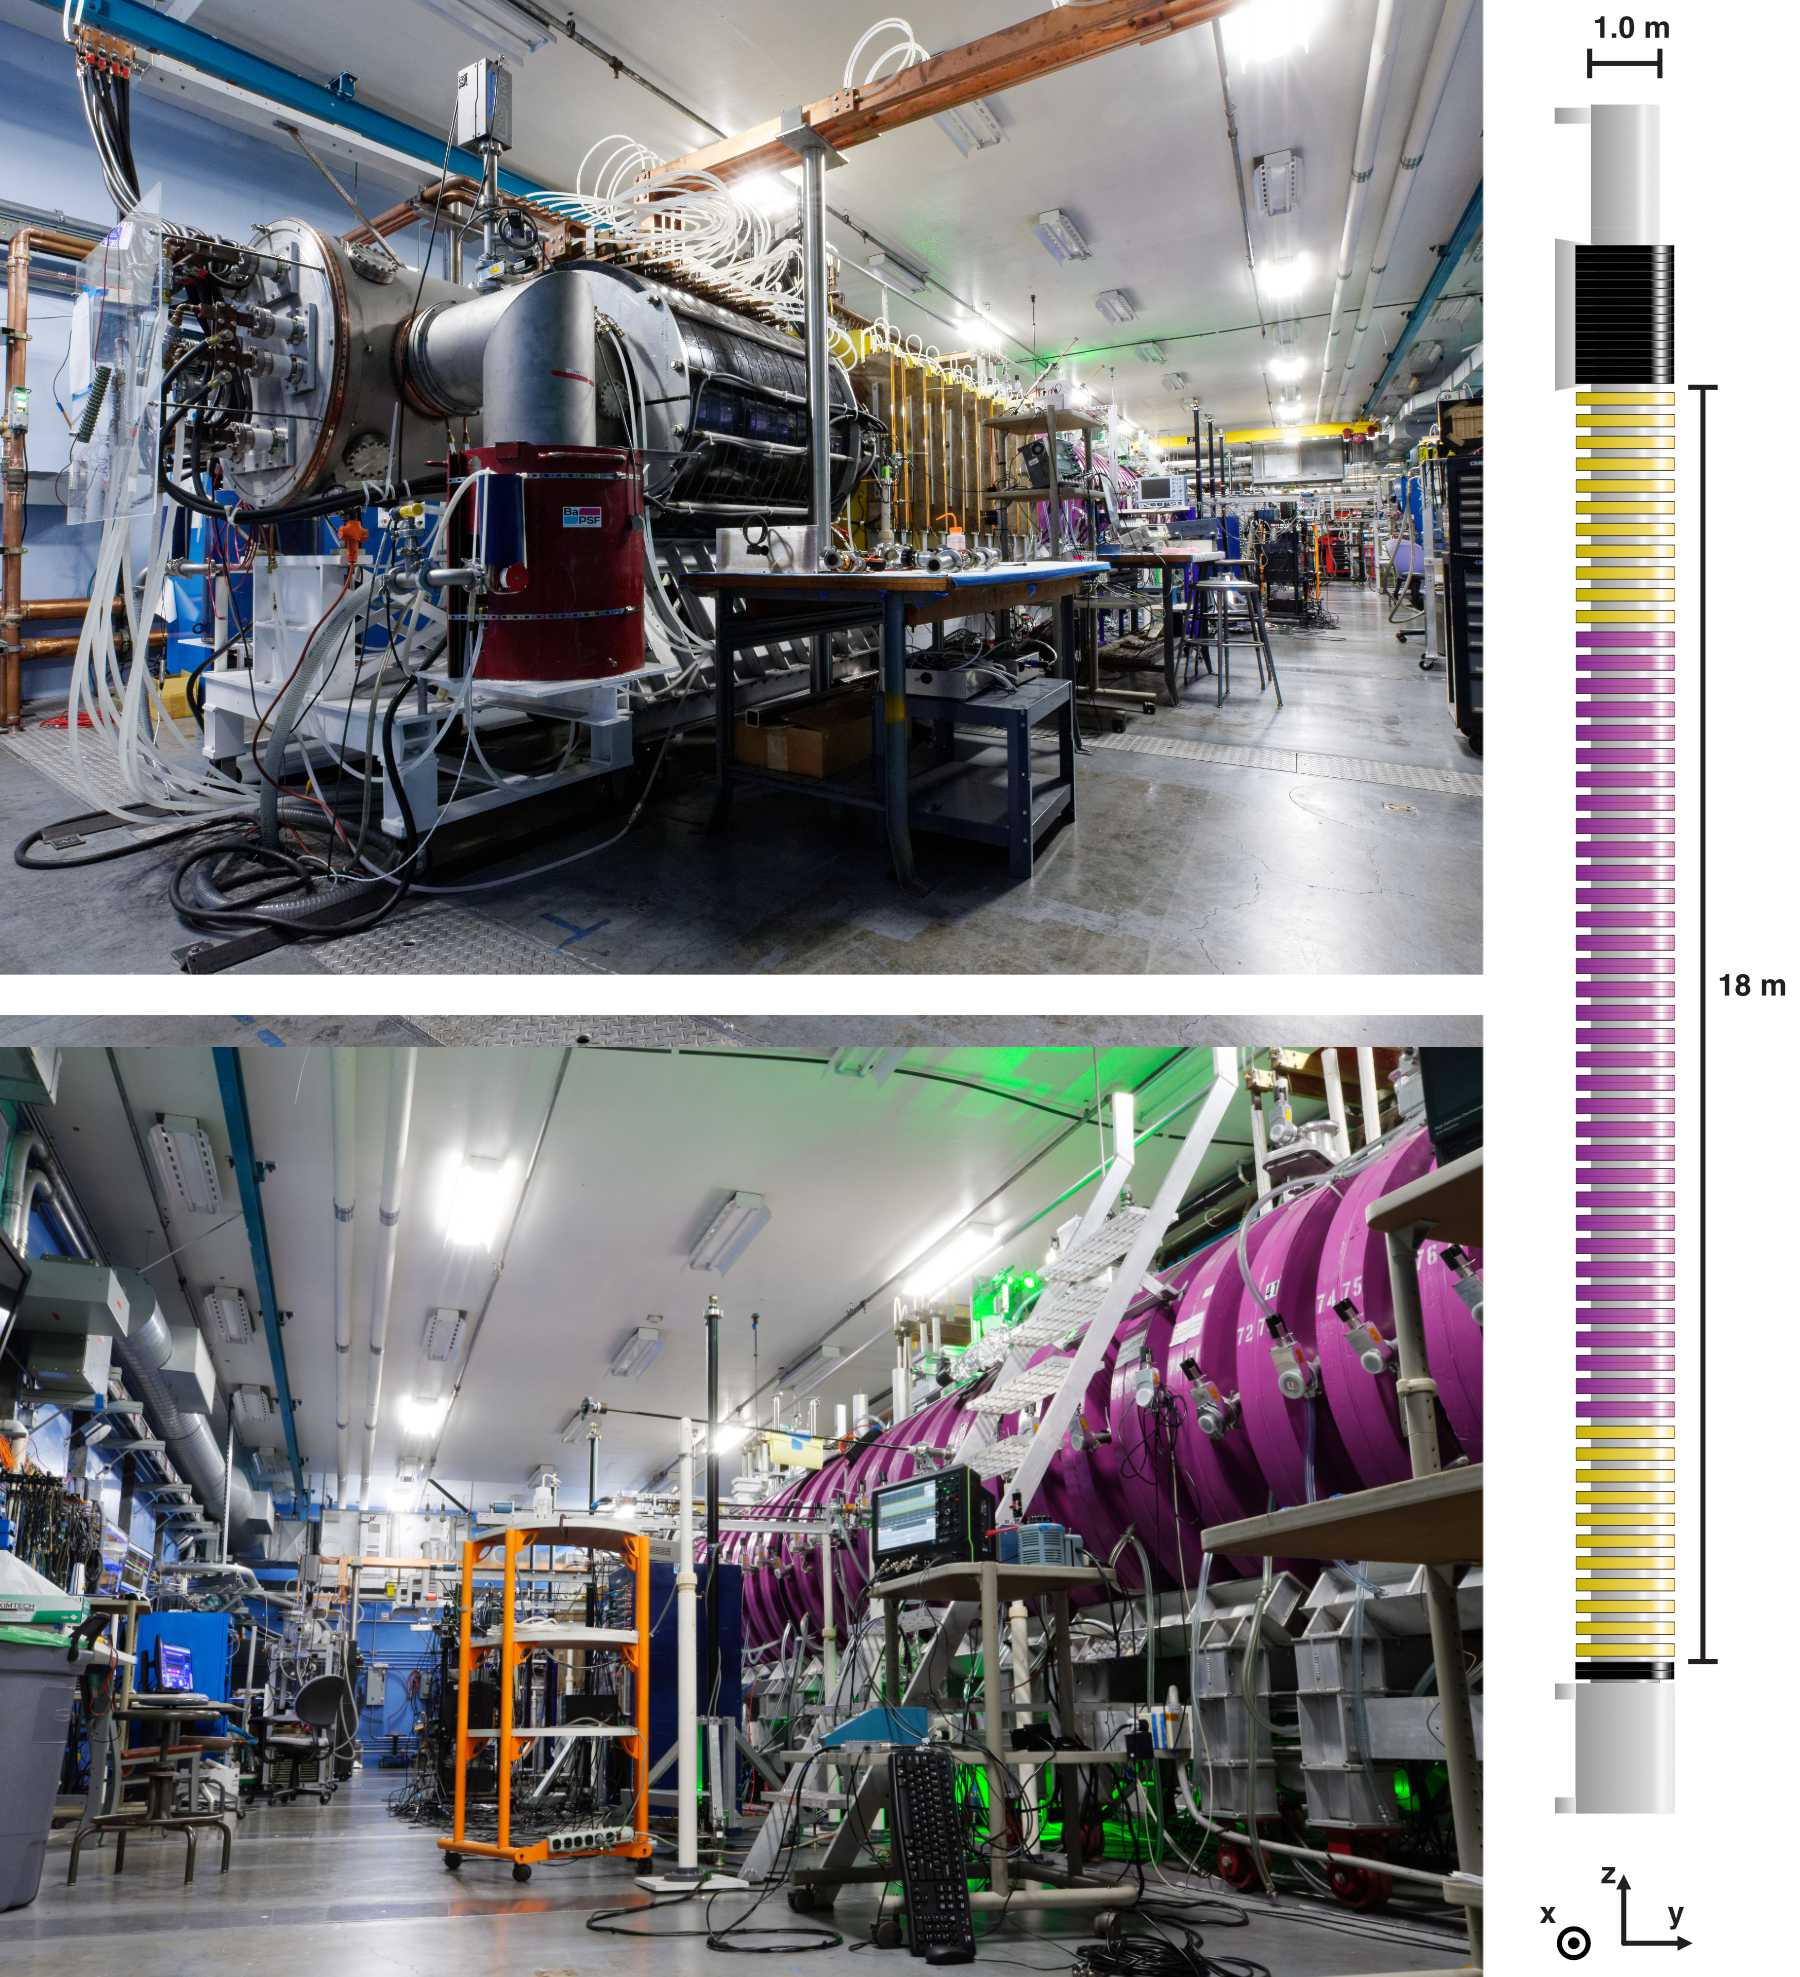
\includegraphics[width=400pt]{figures/lapd_pics.jpg}
	\caption[Pictures of the LAPD]{\label{fig:lapd-pics}Top: picture from the LAPD taken from the south end of the device, next to the cathode and anode region. Bottom: picture taken in the middle section closer to the north end. Right: cartoon of the LAPD with the coordinate system used.}
\end{figure}

\subsection{Plasma source}

Typically, plasmas are produced using a hot cathode and anode at the south end of the device. This cathode was originally barium oxide (BaO)-plated nickel \cite{gekelman_upgraded_2016}, but was recently upgrade to a segmented lanthanum hexaboride (LaB$_6$) source \cite{qian_design_2023}. The BaO cathode was $72$ cm in diameter which mapped to 60 cm in a flat field magnetic field configuration. A $72$ cm diameter, 50\% transparent molybdenum anode was used to accelerate electrons from the cathode down the length of the machine. This BaO source could reach densities of $4 \times 10^{12}$ cm$^{-3}$ and up to 8 eV. The LaB$_6$ cathode is 35 cm across and electrons are accelerated through a 64.4 cm diameter, 66\% transparent molybdenum anode. The LaB$_6$ cathode can form hotter, denser plasmas with densities up to $3 \times 10^{13}$ cm$^{-3}$ and temperatures up to 20 eV, though typical operation yields temperatures around 5 eV, and is also more robust to accidental atmospheric exposure. The LaB$_6$ cathode is heated to $\approx$ 1700 $^\circ$C using a $\approx$2 kA heater. Both of these cathodes were used in the work presented here. An insertable, smaller (20 cm diameter) LaB$_6$ source also exists at the north end of the machine but is not used in this work. An interior shot of the LAPD can be seen in fig. \ref{fig:lapd-inside}.

\begin{figure}
	\centering
	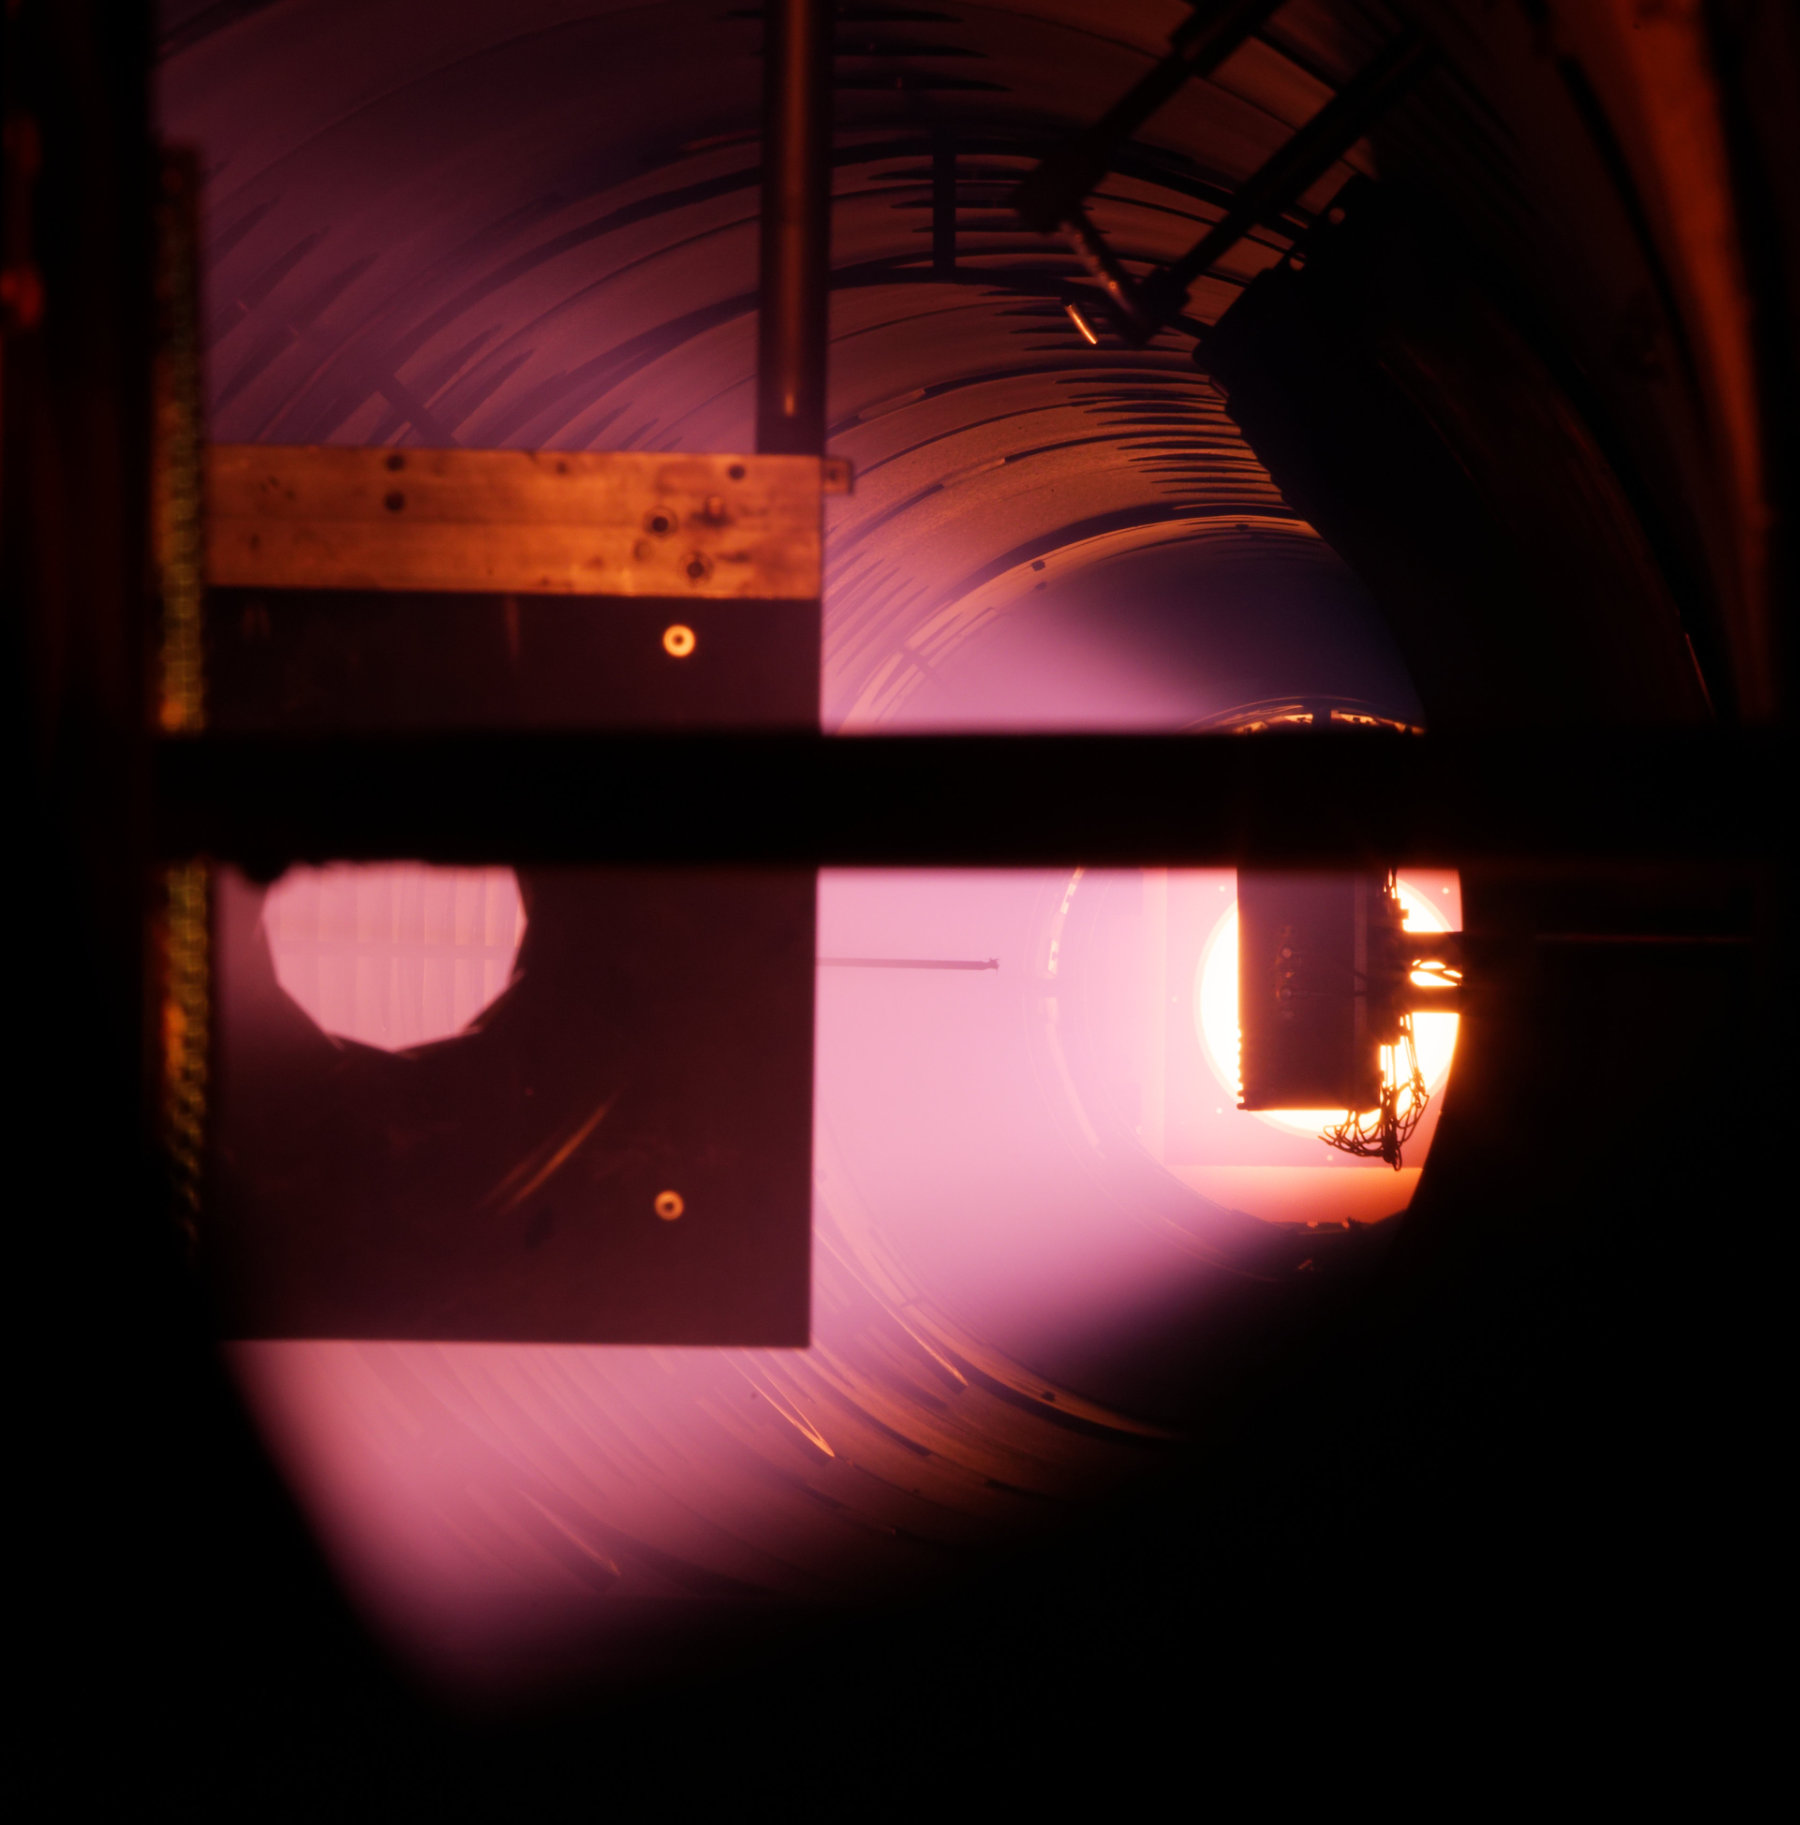
\includegraphics[width=350pt]{figures/lapd_inside.jpg}
	\caption[Picture of LAPD interior]{\label{fig:lapd-inside}The interior of the LAPD taken during a discharge from the end of the machine. The hot LaB$_6$ cathode can be seen at the far end. Inside the plasma chamber are, from left to right, a carbon iris (used in Josh Larson's experiments) for controlling the width of the plasma from the smaller north-end source, an electric dipole probe, and the traveling wave antenna. The pink glow is the plasma formed by the far, main LaB$_6$ source.}
\end{figure}


The voltage applied across the cathode and anode is supplied by a 4.2 Farad capacitor bank switched by group of IGBTs. The discharge voltage is configurable up to 180V before triggering the over-voltage protection, though the capacitors are rated up to 200V. Current through the cathode can exceed 10 kA. Discharges can last as long as 70 ms, though a typical duration is around 15-20 ms. Discharge duration, power, and repetition rate are governed by the size of the capacitor bank and the charging power supply. The discharge repetition rate is configurable between 0.1 and 1 Hz.

\subsection{Magnetic field}
The LAPD has 13 independently-configurable magnet power supplies to shape the geometry of the axial magnetic field. Two of the supplies control the source region field, one controls the north end field where the smaller LaB$_6$ source resides, and the remaining 10 supplies control the field of the main plasma column. The source field can reach up to 8 kG and the main plasma column field up to 1.6 kG. A 1 kG field leads to an ion gyroradius of 2 mm at 1 eV, and a electron gyroradius of 50 $\mu$m at 5 eV, so these plasmas are highly magnetized. The source field is set manually on the power supplies themselves, but the middle 10 fields can be programmed on the LabView housekeeping system.

\subsection{Gas fueling}
There are two main ways of providing the neutral gas necessary for producing plasmas: the static fill system and gas puffing. The static fill system utilizes mass flow controllers to fill the chamber to the desired pressure, usually between $10^{-5}$ and $5 \times 10^{-4}$ Torr. The LAPD can be filled with a variety of (nonreactive) gasses, helium being the most common, followed by hydrogen and argon. The gas puff system utilizes piezo valves to puff gas into the chamber halfway between the cathode and anode. Gas puff duration and valve voltage can be set which influence the total amount of gas puffed and thus plasma density. Plasma  breakdown using gas puffing is very reliable. Without fueling the LAPD has a base pressure of 5 $\times 10^{-7}$ Torr. The pressure is constantly monitored by the housekeeping system. 

\section{Data acquisition}

Probes can sample virtually any point in this plasma through unique ball valves placed every $\approx$32 cm along the length of the device, enabling the collection of time series data with high spatial resolution. Four probe drives can simultaneously be used to move probes in the x-y plane. An x-y-z probe drive is also available for collecting volumetric data. There are also 3 permanently attached probe drives mounted 45$^\circ$ up from the -x axis, on which, at the time of this writing, are mounted Langmuir probes. These drives have a limited motion compared to the standard x-y probe drives used during dataruns and the signals are digitized on 8-bit oscilloscopes. Typically many shots are taken at one position to obtain good sample statistics.

Primarily, probe data acquisition is handled through the main data acquisition system, simply referred to as the ``DAQ''. The DAQ consists of SIS 3302 digitizers (theoretically 32 channels total) capable of sampling signals between $\pm 2.5$ V at 100 MHz at 16 bits. Typically sample averages are taken (16 samples for my data) to reduce data transfer and file size. The DAQ is set up through a LabView-based control system. 

This LabView system manages ``dataruns'' which are a series of discharges with a particular LAPD configuration (including the DAQ, probe motion control, and other device configurations such as function generators). Another LabView system controls the probe movements. All these devices are enabled and commands in a particular order via the run sequencer. 

Another LabView system manages the machine state information (MSI). This system collects information on the discharge (current, voltage), auxiliary diagnostic signals (and it used to record interferometer), gas total pressure and RGA pressures. The time series diagnostics are read by a National Instruments PCIe-6346 data acquisition card which samples with 16 bits over 8 analog inputs at 500 kS/s per input. The MSI also collects information on the state of the magnetic field and cathode heater from the housekeeping system. An auxiliary python system can also be used collate diagnostics from multiple sources, including the machine state information.

\section{Diagnostics}

LAPD can field many different diagnostics and other equipment through the ball-valve ports as well as much larger box-shaped ports.
Probe diagnostics typically go through an isolation amplifier before heading into the DAQ, along with attenuators so the signals fit the DAQ range

\subsection{Langmuir probes: $I_\text{sat}$, sweeps, triple probes}

Langmuir probes (LPs) are a workhorse of diagnostics in low temperature plasmas, such as the LAPD, and are also used at the (lower temperature) edge of fusion devices. These probes can be used to measure density, temperature, and potential of the plasma. LPs are essentially a conductive tip (typically tungsten in our case) inserted into the plasma. Three different types of these LPs can be seen in fig. \ref{fig:langmuir_tips}. 

\begin{figure}
	\centering
	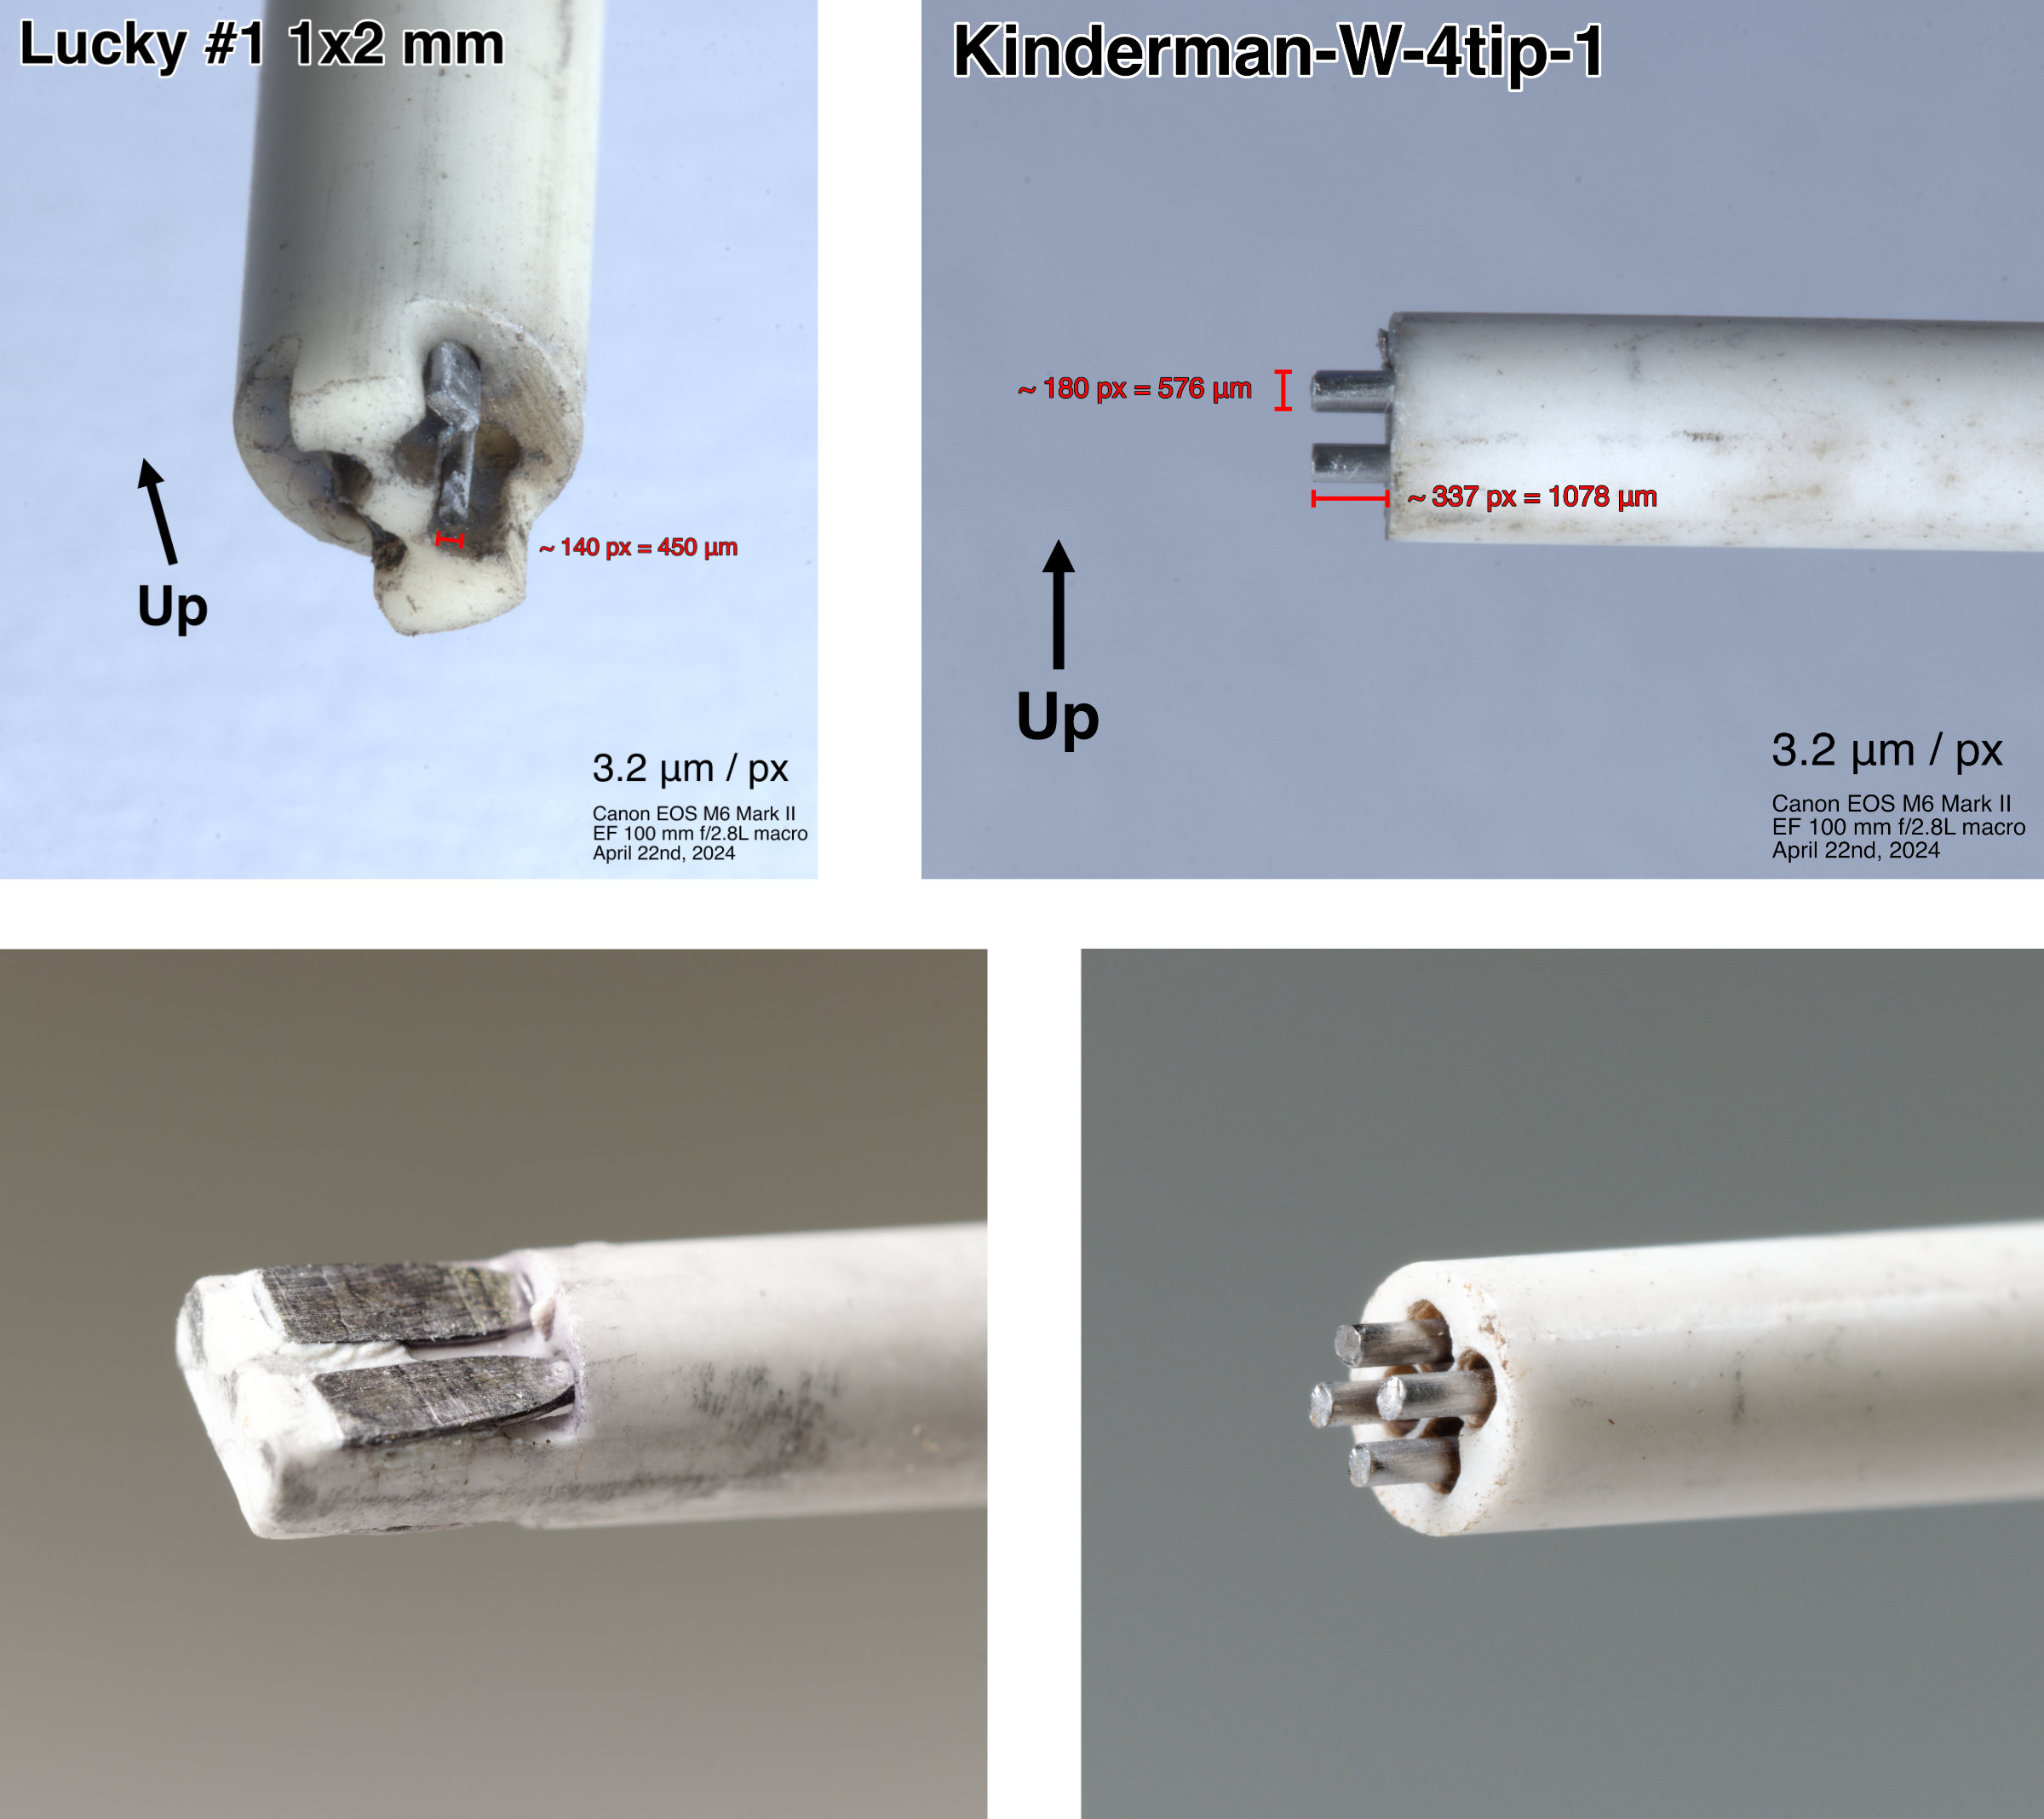
\includegraphics[width=\textwidth]{figures/langmuir_pics.jpg}
	\caption[Images of Langmuir probes used in the LAPD]{\label{fig:langmuir_tips}Three different types of Langmuir probes used in the LAPD: flat protruding tips (top left), flat, flush tips (bottom left), and cylindrical tips (right). Based on measurements using a camera and macro lens, probe areas are often different from what is assumed.}
\end{figure}

The LP can be biased to measure different portions of the current-voltage relationship. Common biasing schemes are: applying a strong negative bias, sweeping the bias along a set range, free-floating the tip, and biasing another tip via the ion saturation current  from another tip. The I-V relationship of a LP and the quantities deduced from it can be seen in fig. \ref{fig:langmuir_sweep} which will be detailed below.

\begin{figure}
	\centering
	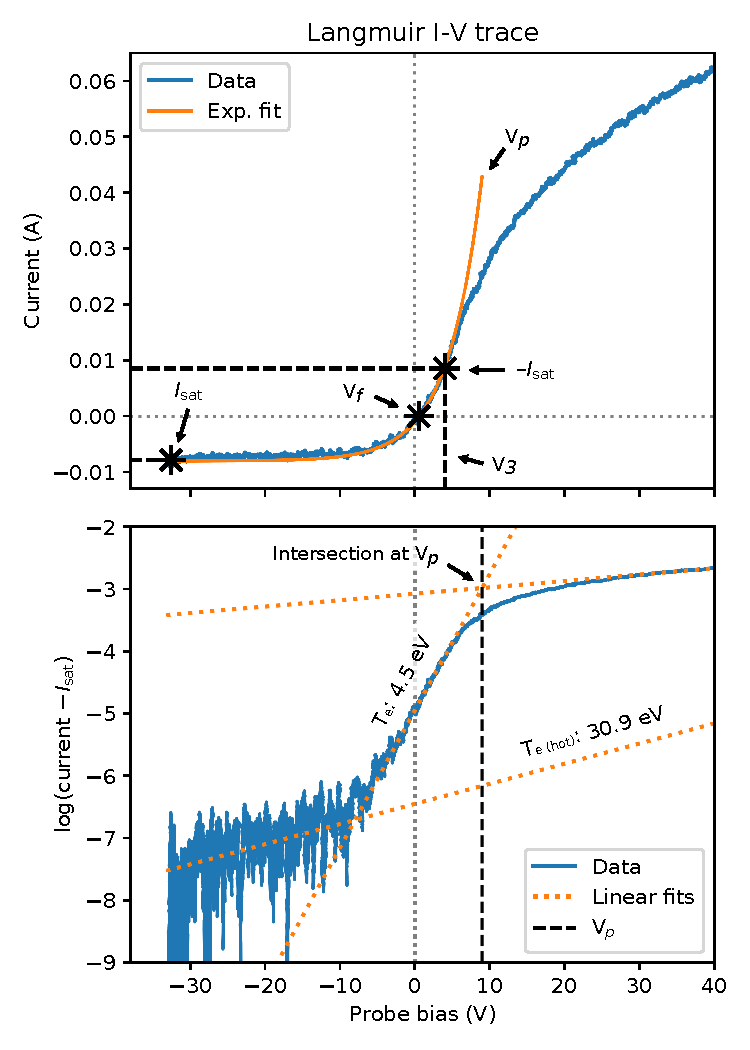
\includegraphics[height=0.8\textheight]{figures/example_sweep_analysis.pdf}
	\caption[Typical Langmuir probe I-V curve]{\label{fig:langmuir_sweep}Typical Langmuir probe I-V curve on top, with a logarithmically-scaled version on the bottom (with $I_\text{sat}$ subtracted). The log-scaled version is typically used for fitting the temperature(s). Useful points on the curve are labeled.}
\end{figure}

\subsubsection{Ion saturation current ($I_\text{sat}$)}
When the LP tip is biased negatively, the probe tips rejects all electrons and only collect ions, and is thus called the ion saturation current. This current, derived from the Bohm sheath criterion for cold ions ($T_i \ll T_e$), is: 
\begin{equation}
	I_\text{sat} = -e^{-1/2} S q_i n_i \sqrt{\frac{T_e}{m_i}}
	\label{eq:isat}
\end{equation}
where $S$ is the effective area, $q_i$ is the charge of the ion, and $n_i$ is the ion density, $T_e$ the electron temperature, and $m_i$ the ion mass.
For a probe tip area of 1 mm$^2$, a current of 1 mA corresponds to $n_e \approx 1\text{-}2\times 10^{12}$ cm$^{-3}$ for a $T_e$ from 4 to 1 eV. The $I_\text{sat}$ on the I-V curve can be seen on the left in the top plot of fig. \ref{fig:langmuir_sweep}. A bias too negative can cause arcing among tips on the same probe shaft. A typical bias is around $-60$ V. 

\subsubsection{Floating potential ($V_f$)}
The floating potential ($V_f$) is the voltage where the probe tip has zero net current, often accomplished by placing a large-valued resistor near the probe tip. This $V_f$ is useful for measuring electrostatic fluctuations, and can also be used as a proxy for plasma potential $V_p$ if the electron temperature $T_e$ is known via the relationship
\begin{equation}
	V_f = V_p - \frac{1}{2} T_e \ln \left( \frac{2 m_i}{\pi m_e} \right)
\end{equation}
In addition, two vertically-arranged $V_f$ tips can be used to approximately measure the local electric field by dividing the difference between the distance between the two probes: $E = (V_{f,\text{top}} - V_{f,\text{bottom}}) / \Delta x$, where $\Delta x$ is the displacement between the probes. This electric field is useful for calculating the local $E\times B$ particle flux.

\subsubsection{Sweeps for $T_e$}
Sweeping the bias applied to a LP tip (within a reasonable range) yields the exponential portion of I-V curve, seen at the top of fig. \ref{fig:langmuir_sweep}. Below the plasma potential, the ion contribution to the curve is $I_\text{sat}$ (eq. \ref{eq:isat}). The electron contribution is (assuming a Maxwellian):
\begin{equation}
	I_e (V_B) = S q_e n_e \sqrt{\frac{T_e}{2 \pi m_e}} \exp \frac{(- q_e (V_p - V_B))}{T_e}
\end{equation}
where $q_e$ is the electron (elementary) charge, $n_e$ the electron density, $m_e$ the electron mass, and $V_B$ the applied bias.

Electron temperature can be determined by fitting this exponential portion, typically by fitting the $I_\text{sat}$-subtracted log-scaled plot seen in the bottom of fig. \ref{fig:langmuir_sweep}. The electron temperature is then the reciprocal of the fitted slope, in this case 4.5 eV. In the LAPD, given the electron beam used to break down the plasma, the electron distribution can have a hot tail which can be fit with a separate curve, which yields 30.9 eV in this case. The electron saturation current region -- the portion of the sweep around $V_B \approx V_p$ and higher -- can be also be fit. The intersection of this line and the temperature fit line is typically considered to occur at the plasma potential $V_p$. 

Plasma potential is useful for calculating the azimuthal velocity profile. The radial electric field can be calculated using a finite differences along a radius, and using the background electric field, the azimuthal $E \times B$ velocity can be calculated. From this the shearing rate can also be calculated.

\subsubsection{Triple probe $T_e$ measurements}
Time-resolved $T_e$ measurements can be obtained by measuring the difference between a probe tip biased by the $I_\text{sat}$ from another probe, called $V_3$ here, and the floating potential. This process effectively measures $T_e$ using three points on the LP I-V curve. These three points (hence, triple probe) can be seen in the top plot of fig. \ref{fig:langmuir_sweep}. At $V_f$, the net current is zero: 
\begin{equation}
	0 = S q_e n_e \sqrt{\frac{T_e}{2 \pi m_e}} \exp \frac{(- q_e (V_p - V_f))}{T_e} + I_\text{sat}
\end{equation}
At $V_3$, the current is $- I_\text{sat}$:
\begin{equation}
	-I_\text{sat} = S q_e n_e \sqrt{\frac{T_e}{2 \pi m_e}} \exp \frac{(- q_e (V_p - V_3))}{T_e} + I_\text{sat}
\end{equation}
(note that $I_\text{sat}$ is a negative quantity).
Combining these two equations and, through some algebra, one obtains $T_e$ as a relationship between $V_f$ and $V_3$:
\begin{equation}
	T_e = \frac{e (V_3 - V_f)}{\ln(2)}
\end{equation}
Given the sensitivity to fluctuations, sweeps are typically more reliable than these triple probe $T_e$ measurements, but they can be relatively accurate. In this case, using the three points from fig. \ref{fig:langmuir_sweep} yields $T_e = 4.48$ eV which is within measurement error of the swept measurement of 4.54 eV. Triple probe measurements require much less post-processing effort than swept measurements because of the difficulty of automating sweep fits. 

\subsection{Magnetic flux (Bdot) probes}

Magnetics measurements are performed using magnetic flux probes, typically called ``Bdots''. Using Faraday's law, a changing magnetic field induces an EMF: $V = - A_\text{eff} \frac{dB}{dt}$, where $A_\text{eff}$ is the effective area of the probe which depends on the area of the loop(s) and the number of turns. These Bdots are formed from three orthogonal loops to capture magnetic fluctuations along all axes. These loops are differentially wound and amplified so that electrostatic effects are removed. The wire is coiled on a ceramic tube which is then covered with a ceramic cap, which can be seen in fig. \ref{fig:bdot-cap}. These probes are calibrated using a Helmholtz coil to measure the spectral response and crosstalk using a network analyzer. For all the signals used in this work, the response of the probe is linear (and remains linear until well into the $\sim$ MHz regime). The construction, calibration, and operation of these probes is covered by Everson et al. \cite{Everson_design_2009}.

\begin{figure}
	\centering
	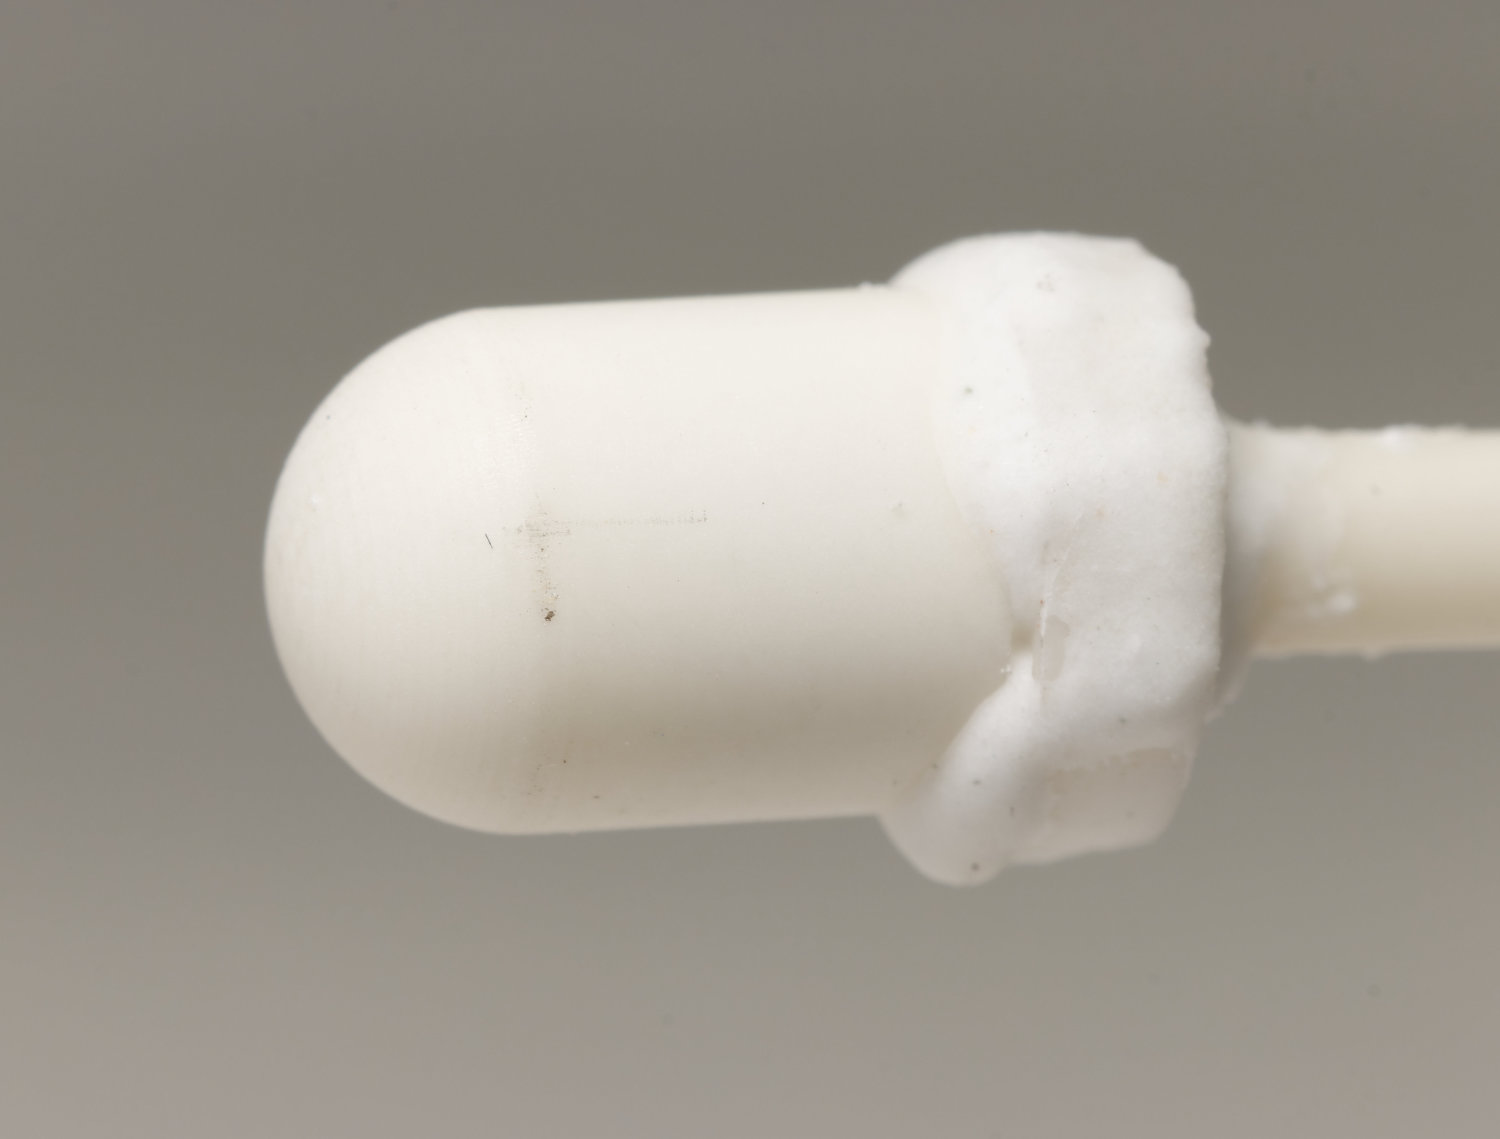
\includegraphics[width=250pt]{figures/bdot_cap.jpg}
	\caption[Ceramic cap of a Bdot probe]{\label{fig:bdot-cap}Ceramic cap of a Bdot probe which is inserted into the LAPD to measure magnetic fluctuations}
\end{figure}

Converting these Bdot signals, after calibration, simply requires integrating $\frac{dB(t))}{dt}$ over time, which is easily accomplished in the frequency domain and avoids accumulating errors. Integrating over $t$ in the frequency domain simply requires dividing by $-i\omega$:

\begin{equation}
	  \int \dot B(t) dt = \int \sum_\omega b_\omega e^{-i \omega t} dt = \sum_\omega \frac{b_\omega}{-i \omega} e^{-i \omega t}
\end{equation}
where $\sum_\omega b_\omega e^{-i \omega t}$ is the Fourier decomposition of $\dot B(t)$

\subsection{The 288 GHz heterodyne interferometer}

The LAPD is equipped with two 288 GHz heterodyne interferometers which measure line-integrated density. These interferometers function by applying a voltage shift to the source of the 288 GHz signal (96 GHz, tripled) using a sawtooth waveform at 750 kHz, leading frequency changes in the range of tens of MHz. Density fluctuations measurable by the interferometer occur much slower than this 750 kHz sweep frequency. When this wave is launched into the LAPD and returned, this 750 KHz wave is phase-shifted relative to a 750 kHz reference caused by both the free-space propagation time and the plasma-induced increased path length. A higher-density plasma leads to an increased path length which leads to a larger observed phase shift. This phase shift can then be unwrapped to obtain a density, given some calibration factor. The reference and detector signals are recorded by an oscilloscope, which can be read from LabView (as part of the MSI system) or python, or written to a file.

\subsection{Thomson scattering}

Thomson scattering is the gold standard of temperature measurements. In the LAPD, the Thomson scattering has been implemented in the non-collective regime using a 532 nm, 460 mJ Nd:YAG laser to measure $T_e$ and $n_e$ \cite{ghazaryan_thomson_2022}. Thomson scattering is the process of electrons scattering and doppler shifting incident light, where the doppler shift is caused by the electron thermal motion. This scattered light is then collected by a spectrometer where the doppler shift is directly measured. The density can also be measured by counting the incident photons after absolute calibration of the entire optical system, including scanning of the fiber coupling optics to maximize signal. Between shots, background spectra are taken and subtracted from the signal to reduce the influence of optical imperfections and spurious light. A notch filter is also used to block reflections from the 532 nm laser.

Analysis is fairly straightforward: the spectrum can be fit assuming a Gaussian distribution if the plasma distribution is Maxwellian. The temperature is determined by the width of the distribution: $T_e = 0.4513 \cdot \Delta \lambda_{1/e}^2$, where $\lambda_{1/e}$ is the half width where the spectrum reduces by $1/e$ \cite{ghazaryan_thomson_2022}. The density can be calculated by integrating this fit distribution, but without a recent and accurate absolute calibration this value is not reliable and should not be used.

The Thomson scattering system benefits from higher density (above $10^{13}$ cm$^{-3}$) and lower temperatures, otherwise many shots (a few thousand) may be required to get a spectrum with a desirable fitting accuracy. Presently, this system measures temperature on-axis at port 32 at a single point in time (span of 4 ns) in the plasma. The measurement volume can be moved to elsewhere in the device with great effort. Coincidentally, a Helium ion line ($7 \rightarrow 4$ transition) at 541 nm is occasionally visible on the spectrum, but the resolution of the spectrometer (0.28 nm) is not sufficient to calculate a thermal doppler shift for reasonable ion temperatures, but it could provide an upper bound.

\subsection{Fast framing camera}

The facility currently has a Phantom v7.3 fast framing camera. At 800 by 600 resolution, it can record at 6,688 frames per second, but can record at over 35,000 frames per second at a 256 by 256 resolution. The camera sensor is 14 bit monochrome and capable of resetting pixels and reacquiring light on event of sensor saturation (the ``extreme dynamic range'' feature). Although this footage is not analyzed in a quantitative way, it is nonetheless useful for building intuition on the structures and dynamics in the device (and worst case, makes for some pretty images). The light collected by the camera has been shown to correlate fairly well with $I_\text{sat}$, at least in the plasma bulk (according to unpublished work by Daniel Guice). 

\section{Instabilities in mirrors and the LAPD}

\subsection{Drift waves}

Drift waves exist in any magnetized plasma that has a density gradient. For this reason, this is often called a ``universal'' wave or instability. 

Pressure gradient in a slab
Any resistivity leads to charge separation and instability growth
Show diagram 

\subsection{Rotational interchange}



\subsection{Interchange}

Pressure gradient aligned with curvature vector
Showstopper for earlier mirror machines

\section{Machine learning and neural networks}

Fundamentally, neural networks (NNs) are a function that, given sufficient capacity, can represent any function -- this is the ``universal approximation theorem''. Stated succinctly, NNs are fancy curve fits. As we will see in this work, fancy curve fits can be very useful.

\subsection{Fundamentals of neural networks}

Neural networks are built one `layer' at a time. A layer in an NN is a vector $\vec x_i$ multiplied by some weight matrix $\mathbf{W}$ followed by a nonlinearity to get the activation $x_{i+1}$:
\begin{equation}
	\vec x_{i+1} = f( \mathbf{W} \vec x_i)
\end{equation}
where $\vec x_i$ is the previous activation (or input). A bias $b$ (a learnable offset) is often concatenated to the input vector beforehand. The activation function $f$ can be any nonlinearity. Typical choices for $f$ include the rectified  linear unit -- ReLU (zero when the input is less than zero, linear otherwise), tanh, sigmoids, sigmoid linear unit (SiLU), and so on. ReLU, and a variant of which called Leaky ReLU, are popular choices given the simplicity of computation.

Stacking these layers one after another leads to the ability to express very complex curves. The true innovation here is the ability to express very high dimensional curves which was otherwise impossible until the advent of modern NN techniques, enabled by fast matrix multiplication hardware (read: GPUs).

The weights of these layers are trained via gradient descent of some loss function $\mathcal{L}$. The loss is effectively the penalty for the network predicting the incorrect answer. A typical loss function for regression tasks is the mean-squared error: 
\begin{equation}
	\mathcal{L} = \frac{1}{M} \sum_{i=1}^M (x_i - g(x_i))^2
\end{equation}
where $g(x)$ is the output of the neural network and $x_i$ is a training example in a batch size M. Training over a dataset is often done in batches to reduce the memory required and to introduce stochasticity into the training process which can improve generalization. 

Gradient descent is the process of modifying the NN weights by calculating the gradient of the loss function with respect to those weights:
\begin{equation}
	\theta \gets \theta - \nabla_\theta \mathcal{L}
\end{equation}
Advanced purpose-built algorithms exist to do this gradient descent in a fast manner, the most popular being Adaptive Moment Estimation, known as Adam  \cite{kingma_adam_2017}. 


\subsection{Common layer types}

In this work we use three types of NN layers. First is the dense layer, also referred to as a ``fully-connected'' layers or ``multilayer perceptron'' if the entire model uses dense layers. In this layer every input is connected to every output. This fully-connected topology can lead to very large parameter counts if these layers are repeatedly stacked with a large width.

Second: the convolutional layer, or convolutional neural network (CNN) \cite{lecun_convolutional_1995}. This layer scans along the input with a smaller NN. The input dimension of this layer is the ``kernel size'', and the different networks scanning across the input are the ``filters''. These CNNs have been used to great effect in image processing and time series analysis and are relatively parameter-efficient.

Third: the attention layers. These layers have three inputs called the query, key, and value. When these are all the same the mechanism is called ``self-attention''. The query and key are matrix-multiplied and converted to a probability distribution via a softmax function. This softmax result is then applied to the value, yielding scaled dot product attention \cite{vaswani_attention_2017}: 
\begin{equation}
	\text{Attention}(Q, K, V) = \text{softmax}\left( \frac{QK^T}{\sqrt{d_k}} \right)V
\end{equation}
where $d_k$ is the dimension of the query and key.
The result of this combination is mask that selects important parts of the value vector. Stacking many of these layers, with multiple self-attention mechanisms for the same input vectors, creates a ``transformer'' \cite{vaswani_attention_2017} which is the basis for the recent advancements in large language models. 
%Here we use these attention mechanisms more modestly.

\subsection{Generative models}
Generative models are models that learn a joint probability distribution over the inputs $X$ and outputs $Y$, $p(X, Y)$  instead of learning the conditional distribution $p(y \vert X=x)$ which are ``discriminative'' models. Models that produce a single point estimate are also considered to be discriminative. The learned joint distribution can typically be sampled both unconditionally (generating realistic-looking data) or conditionally to generate samples when given additional information. A brief overview of most commonly used generative models in fusion will be given here. Common generative architectures are variational autoencoders (VAEs), generative adversarial networks (GANs), diffusion models, autoregressive models, and energy-based models (EBMs).

A VAE \cite{kingma_auto-encoding_2022} is composed of an encoder network and a decoder network. The model is trained by mapping the encoder output to a latent probability distribution. This probability distribution can then be sampled by the decoder. The model is trained by minimizing the difference between the data distribution and the sampled distribution (such as using the Kullback-Leibler divergence) and also minimizing the reconstruction error.

A GAN \cite{goodfellow_generative_2014} is composed of an explicit generator network that generates plausible samples, and a discriminator network that distinguishes between generated samples and data. The generator is trained on how well it fools the discriminator, and the discriminator is trained on how well it can discriminate between generated samples and real data. These two optimizations compete.

Diffusion models \cite{ho_denoising_2020} work in a somewhat different way compared to GANs and VAEs. The diffusion model functions by iteratively adding noise to an image such that the image converges to a Gaussian. An NN is then trained to invert this noising process, enabling sampling from a distribution from pure noise. 

Autoregressive models, usually for time-series data or language modeling, predict the next item in a sequence given an earlier (set of) items. This model is the main idea behind training of large language models -- so called ``generative pretrained transformers'', or ``GPT'' \cite{radford_improving_2018}. 

Energy-based models parameterize the probability distribution via an energy function where the probability is defined as $p =\exp(-E) / Z$, where Z is the partition function. These are trained by evaluating the log-likelihood of the probability to get contrastive divergence. 

\section{Machine learning in plasma science}

\section{ML in ICF}

\section{ML for control}





























\graphicspath{{Chapters/Chapter_mirror-turb/}}

\chapter{Turbulence and transport in mirror geometries in the Large Plasma Device}
\label{ch:mirror_turbulence}

%\bibliographystyle{apsrev4-2}

% markers (black, blue, brown, cyan, darkgray, gray, green, lightgray, lime, magenta, olive, orange, pink, purple, red, teal, violet, white, yellow, more: https://en.wikibooks.org/wiki/LaTeX/Colors)
%\newcommand{\marker}[3]{
%  \tikz[baseline=(X.base)]{
%    \node[fill=#1!40,rounded corners] (X) {#2:};
%  }
%  {\color{#1!80!black}#3}
%}
% make new commands here
%\newcommand{\phil}[1]{\marker{cyan}{phil}{#1}}  % Phil
%\newcommand{\troy}[1]{\marker{green}{Troy}{#1}}  % Troy
%\newcommand{\todo}[1]{\marker{orange}{TODO}{#1}}  % Phil

%\begin{document}

%\preprint{AIP/123-QED}

%\title[]{Turbulence and transport in mirror geometries in the Large Plasma Device}
% Force line breaks with \\

%\author{Phil Travis}
% \email{phil@physics.ucla.edu}
%\author{Troy Carter}
%  \email{tcarter@physics.ucla.edu}
%\affiliation{ 
%University of California, Los Angeles Department of Physics and Astronomy
%}

%\date{\today}

\begin{abstract}

In this chapter we study turbulence and cross-field particle transport in LAPD mirror configurations. 
%Cross-field transport and turbulence in mirrors remains relatively understudied compared to toroidal devices. 
%Turbulence and transport in mirror configurations were studied utilizing the flexible magnetic geometry of the Large Plasma Device (LAPD). 
Mirror machines are once again rising in prominence as a candidate for commercial fusion reactors with the advent of highly-funded commercial ventures and high-field high-temperature superconducting magnets \cite{WHAM, BEAM}, so development of a functional understanding of cross-field transport in mirrors is imperative. 
Using the LAPD, multiple mirror ratios from $M=1$ to $M=2.68$ and three mirror-cell lengths from $L=3.51$m to $L=10.86$m were examined.
Langmuir and magnetic probes were used to measure profiles of density, temperature, potential, and magnetic field. The fluctuation-driven $\tilde{E} \times B$ particle flux was calculated from these quantities. Two probe correlation techniques were used to infer wavenumbers and two-dimensional structure.
Cross-field particle flux and density fluctuation power decreased with increased mirror ratio.
Core density and temperatures remain similar with mirror ratio, but radial line-integrated density increased.
The physical expansion of the plasma in the mirror cell by using a higher field in the source region may have led to reduced density fluctuation power through the increased gradient scale length. This increased scale length reduced the growth rate and saturation level of rotational interchange and drift-like instabilities.
Despite the introduction of magnetic curvature, no evidence of mirror driven instabilities — interchange, velocity space, or otherwise — were observed. For curvature-induced interchange, many possible stabilization mechanisms were present, suppressing the visibility of the instability.

This chapter is based on my 2025 publication in the Journal of Plasma Physics titled ``Turbulence and transport in mirror geometries in the Large Plasma Device'' \cite{travis_turbulence_2025}.
\end{abstract}

\section{\label{sec:intro}Introduction}

Historically, mirror research has prioritized the main issues with mirror confinement: stabilizing the interchange instability, stabilizing velocity-space (loss-cone-driven) instabilities, and minimizing axial electron heat losses. Nevertheless cross-field transport remains an important topic in magnetic-confinement fusion reactor development, in both linear and toroidal geometries. Insight into edge-relevant turbulence, and its coupling to interchange and other mirror-driven instabilities, performed in a basic plasma science device may be useful for a mirror-based reactor. Although not at fusion-relevant core temperatures or densities, the Large Plasma Device (LAPD) operates at conditions similar to the edge of fusion devices and can provide insight into the physical processes in that region. 
A characterization of edge fluctuations has been undertaken, with emphasis on interpreting these fluctuations within the context of mirror. 

Non-classical cross-field particle transport is often caused by low-frequency, large-amplitude fluctuations. These fluctuations are the result of various instabilities. One such process is the "universal" drift instability, which appears in the presence of a density gradient and finite resistivity. Drift wave turbulence and the effect on transport has been extensively studied in the past \cite{Horton_1999, Tynan_review_2009}. In the presence of sufficiently high rotation or sheared flow, rotational interchange and the Kelvin-Helmholtz instabilities also contribute or couple to these fluctuations. 

Various gradient-, rotation-, and shear-driven instabilities (and suppression of such) have been studied previously in the LAPD experimentally \cite{Schaffner_2012, Schaffner_turbulence_2013, Schaffner_2013} and in simulations using BOUT, a 3d fluid turbulence code, and an eigenvalue solver \cite{Popovich_2010}. The LAPD has a sufficiently high spontaneous rotation rate that rotation-driven instabilities may be excited without artificial drive. Simulations using BOUT++ \cite{Friedman_2013} have also suggested that a rapidly growing nonlinear instability may dominate over all other linear instabilities.

Imposing a magnetic mirror configuration introduces magnetic curvature. The alignment of the curvature vector with a pressure gradient vector component causes the flute-like interchange instability if no stabilization mechanism is present. This interchange mode could couple to finite $k_\parallel$ drift waves. The coupling of drift waves to curvature-induced interchange modes has been studied in toroidal devices such as TORPEX \cite{Poli_experimental_2006, Fasoli_electrostatic_2006}, where curvature was seen as the driving component for the unstable drift-interchange modes. Drift-like fluctuations have also been observed in the GAMMA-10 mirror \cite{Mase_1991, Yoshikawa_2010}. Flute-like modes and drift waves have been studied in other linear devices, such as Mirabelle \cite{Brochard_transition_2005}, where the appearance of flute-like modes or drift waves were controlled by varying the field and limiter diameter. 

The rotational interchange and curvature interchange can both be flute-like modes. Rotational interchange (also called the ``centrifugal instability") is driven by the aligned centrifugal force and pressure gradient vectors, but curvature-driven interchange is instead driven by magnetic curvature and is typically referred to as simply the ``flute" or ``interchange" instability. Rotational interchange \cite{Jassby_transverse_1972} has been observed in the LAPD in the past \cite{Schaffner_2012, Schaffner_2013}, and the curvature-driven interchange instability has been observed in many other mirror machines \cite{wickham_curvature-induced_1982, ferron_interchange_1983, Post_1987}. 

Biasing or modifying the electrical connection of the plasma with the end wall has proven to be a important actuator in many mirror machines such as TMX-U \cite{Hooper_1984}, GAMMA-10 \cite{Mase_1991}, and GDT \cite{Bagryansky_2003, Bagryansky_2007, Beklemishev_2010}, and will be utilized on WHAM \cite{WHAM}. Active biasing was not attempted in this study, but the intrinsic rotation and strong electrical connection to the source region may provide a useful analog for edge biasing in other mirror machines.

The LAPD exhibits a high degree of turbulence so it is difficult to identify the dispersion relation of the modes that are present. Nevertheless, the LAPD has good coverage of perpendicular spectra using correlation-plane techniques, and some measure of parallel spectra using the correlation between two axially-separated probes. A space-time spectral characterization of the many instabilities present in this low beta, moderate aspect ratio, gas-dynamic trap regime is attempted.

This goal of this study was to investigate the changes to turbulence and transport in LAPD mirror configurations. Of particular interest were the potential coupling of the interchange instability with drift waves or other modes, and the effect of the mirror geometry on cross-field particle flux. Presented is a characterization of the observed modes and the effect of introducing a mirror geometry.
This paper is organized as follows. Sec. \ref{sec:methods} discusses the configuration of the LAPD and the diagnostics used. Sec. \ref{sec:changes} covers the changes seen when imposing a magnetic mirror configuration on profiles, particle flux, drift waves, turbulence, and magnetic fluctuations. Sec. \ref{sec:structure} explores the changes in 2d (x-y plane) structure. Sec. \ref{sec:discussion} discusses the active and expected instabilities and reasons for their modification. Sec. \ref{sec:conclusion} summarizes the study and discusses the requirements for a deeper investigation.

\section{\label{sec:methods}The experiment and device configuration}

\subsection{\label{sec:sub_exp}The Large Plasma Device (LAPD)}
%The Large Plasma Device (LAPD) is a 20 meter long, 1 meter diameter basic plasma device at UCLA \cite{LAPD_BaO}. The LAPD has a variable magnetic field, from 250G to 1.6 kG and can be varied axially. Probes inserted into the plasma can collect high-resolution, temporal information on density, temperature, potential, and magnetic field fluctuations. 

In this study, the plasma was formed using an emissive, $72$ cm  diameter barium-oxide (BaO) cathode \cite{LAPD_BaO} (mapped to 60 cm in a flat field) and a $72$ cm diameter, 50\% transparent molybdenum anode that accelerate electrons across a configurable $40-70$V potential; voltages of $60$ and $63$V were used in this study. The source has since been upgraded to a lanthanum hexaboride (LaB6) cathode \cite{LAPD_LaB6} that enables access to higher-density, higher-temperature regimes, but all the data in this study are from plasma formed by a BaO cathode. 

The flexible magnetic geometry of the LAPD was used to construct a variety of magnetic mirror configurations. The discharge current, fill pressure, and other machine parameters were held constant. The typical plasma parameters observed in this study can be seen in table \ref{tab:plasma-parameters}. 
Data in several mirror ratios and lengths were collected (see table \ref{tab:fields}) but emphasis is placed on the short cell because the highest mirror ratio possible ($M=2.68$) with a $500$ Gauss midplane field could be accessed and probes were able to be placed outside of the mirror cell. An overview of the axial magnetic field for the the short mirror configurations and probe locations can be seen in fig. \ref{fig:magnetic_geometry}. 2- or 3-cell mirror configurations were also explored but are not examined in this study. All results presented below are from the short mirror cell configuration unless otherwise specified.

\begin{figure*}
    \centering
    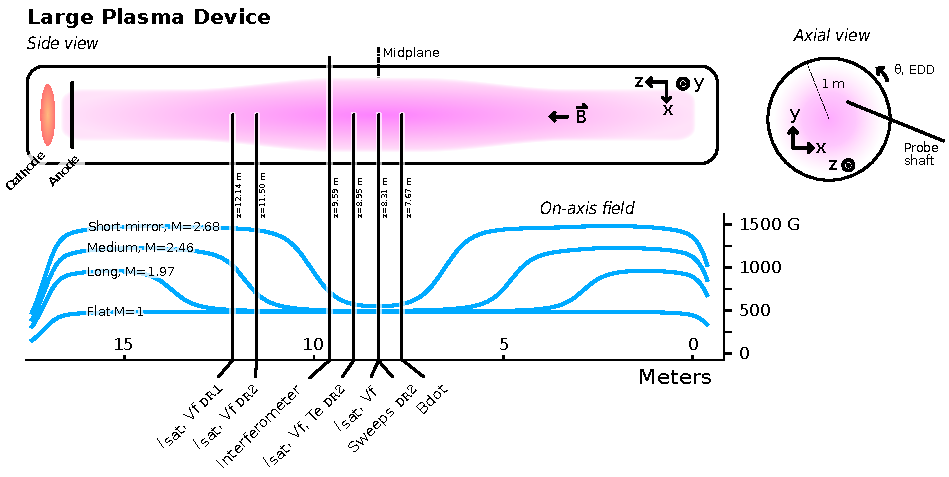
\includegraphics[width=\textwidth]{figures/fig1.pdf}
    \caption{Cartoon of the Large Plasma Device and the coordinate system used. Only four of the eleven mirror configurations studied are plotted for clarity (mirrors of the same length have similar shapes and simply scale with mirror ratio). Diagnostic set varied by datarun; unlabeled diagnostics were used in both dataruns.}
    \label{fig:magnetic_geometry}
\end{figure*}

\begin{table}
 \centering
 \begin{tabular}{l l l l l}
 Mirror length & \multicolumn{4}{l}{Mirror ratios ($M$)} \\
 \hline
 Flat & 1 & & & \\
  3.51 m (short) & 1.47 & 1.90 & 2.30 & 2.68 \\ 
 7.03 m (medium) & 1.49 & 1.98 & 2.46 & \\
 10.86 m (long) & 1.47 & 1.97 & 2.44 & \\
 \end{tabular}
\caption{\label{tab:fields}Magnetic mirror lengths and ratios. The lengths are measured where the curvature changes sign and the ratio is the maximum divided by the minimum. Approximately $3.5$m must be added to the length if the good-curvature region is included. In the case of small asymmetries, the field strengths were averaged before calculation of the mirror ratio.}
\end{table}

\subsection{\label{sec:sub_diagnostics}Diagnostics}

All diagnostics were recorded with a effective sampling rate of 6.25 MHz (16-sample average at 100 MSPS) and a spatial resolution of 0.5 cm. When necessary, averaging over time is done in the approximate steady-state period of the plasma discharge ($4.8$ to $11.2$ ms from the $1$ kA trigger signal). Unless otherwise noted, all data presented will be from probes inside the mirror region ($z \approx 7$m). An example of a raw $I_\text{sat}$ signal and processing steps can be seen in fig. \ref{fig:raw-signals-plots}. The raw signals are detrended by subtracting the mean across shots to obtain the fluctuations only. FFTs are then taken of these fluctuations for calculating power spectra and cross-correlated quantities. Frequencies above 200 kHz are dominated by electronics and instrumentation noise and thus are also ignored. Fluctuation power profiles can then be constructed.

\begin{figure}
    \centering
    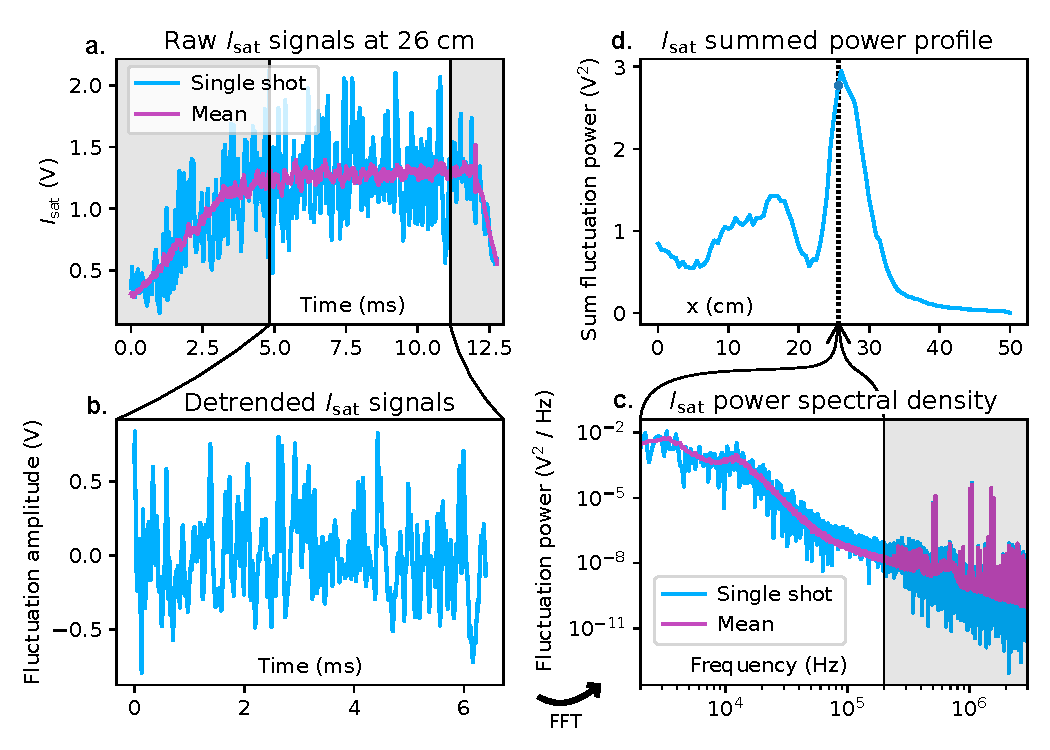
\includegraphics[width=\textwidth]{figures/fig2.pdf}
    \caption{Raw data and basic processing steps for LAPD probe diagnostics as demonstrated by an $I_\text{sat}$ trace from a \texttt{DR1}, $M=1$ mirror at 26 cm. Data are truncated from 4.8 to 11.2 ms (a) and detrended (b). Power spectral density is calculated (c), and a power profiles can be constructed (d). The shaded regions are excluded from this analysis.}
    \label{fig:raw-signals-plots}
\end{figure}

The data presented were collected in two phases. The first phase ("datarun"), \texttt{DR1}, collected Langmuir probe ($I_\text{sat}$ and Vf) and magnetic fluctuation ("Bdot") \cite{Everson_design_2009} traces. 50 shots were taken at each position for every configuration. 
The second phase, \texttt{DR2}, was conducted with a similar set of diagnostics focused on temperature measurements (swept and triple probe) and 2d x-y structure. 15 shots were taken at each position, except for Langmuir sweeps with 64 shots. When appropriate, all data for each position were shot-averaged.
"$I_\text{sat}$" will be used interchangeably with "density" and be presented with units of density (assuming a flat $T_e = 4.5$ eV profile).

\begin{table}
    \centering
    \setlength\extrarowheight{-6pt}
    \begin{tabular}{l l l l l}
        Cathode radius (M=1) & $x_c$ & $30$ && cm \\
        Machine radius & $R$ & $50$ && cm \\
        Plasma length & $L$ & $\sim 17$ && m \\
        Primary species && He-4 1+ \\ 
        Electron-helium mass ratio && $1.37 \times 10^{-4}$ \\
        Neutral pressure && $6 - 20 \times 10^{-5}$ && Torr \\
        \hline
        Quantity &  & Core & $x=x_\text{PF}$ & Unit \\
        \hline
        Density & $n_e$ &  $1.25 \times 10^{12}$ & $ 0.6 \times 10^{12}$ & $\text{cm}^{-3}$ \\
        Ion temperature & $T_i$ & $\sim 1$ & — & eV \\
        Electron temperature & $T_e$ & $4$ & $5$ & eV \\
        Beta (total) & $\beta$ & $9 \times 10^{-4}$ & $6 \times 10^{-4}$ & \\
        Midplane magnetic field & $B_\text{mid}$ & $500$ & — & G \\
        Plasma freq & $\Omega_{pe}$ & $10$ & $7.1 $& GHz \\
        Ion cyclotron freq & $\Omega_{ci}$ & $200$ & — & kHz \\
        Electron cyclotron freq & $\Omega_{ce}$ & $1.4$ & — & GHz \\
        Debye length & $\lambda_D$ & $0.013$ & $0.021$ & mm \\
        Electron skin depth & $\lambda_{e}$ & $30$ & $43$ & mm\\
        Ion gyroradius & $\lambda_{ci}$ & $5.8$ & — & mm \\
        Electron gyroradius & $\lambda_{ce}$ & $0.13$ & 0.15 & mm \\
        Ion thermal velocity & $\bar{v}_i$ & $6.94$ & — & km/s\\
        Electron thermal velocity & $\bar{v}_{e}$ & $1190$ & $1330$ & km/s \\
        Sound speed & $c_s$ & $13.0$ & $13.9$ & km/s\\
        Alfvén speed & $v_a$ & $446 - 1140$ & $ - 1620$ & km/s \\
        Ion sound radius & $\rho_s$ & $65$ & $69$ & mm\\
        Ion-ion collision freq & $\nu_{ii}$ & $730$ & $380$ & kHz \\
        Electron-ion collision freq & $\nu_{ei}$ & $6.77$ & $2.59$ & MHz \\
        Electron collision freq & $\nu_{ee}$ & $9.57$ & $3.66$ & MHz \\
        Ion mean free path & $\lambda_{i,\text{mfp}}$ & $26$ & $50$ & mm \\
        Electron mean free path & $\lambda_{e, \text{mfp}}$ & $175$ & $512$ & mm \\
        Spitzer resitivity &  $\eta$ & $192$ & $146$ & \SI{}{\micro \ohm \meter} \\
        
    \end{tabular}
    \caption{LAPD machine information and plasma parameters in the core and peak-fluctuation region ($x=x_\text{PF}$) at the midplane in this study. Dashed quantities are assumed to be identical to core quantities.}
    \label{tab:plasma-parameters}
\end{table}

\section{\label{sec:changes}Mirror-induced changes}

\subsection{Profile modification}

\begin{table}
    \centering
    \begin{tabular}{c c c c c c}
         Mirror ratio & 1 & 1.47 & 1.90 & 2.30 & 2.68 \\
         \hline
         Scale factor & 1 & 1.21 & 1.38 & 1.52 & 1.64\\
         $x_{c}$ (cm) & 30 & 36 & 41 & 45 & 49 \\
         $x_{PF}$ (cm) & 26 & 32 & 36 & 40 & 43 \\
    \end{tabular}
    \caption{$x_c$ and $x_{PF}$ locations for each mirror ratio when scaled by the expected magnetic expansion.}
    \label{tab:x_PF}
\end{table}

Because the field at the plasma source increases with $M$, the midplane plasma expands by a factor of $\sqrt{M}$. The physical locations of the peak fluctuation region -- $x_{PF}$ (maximum gradient) -- and the cathode radius $x_c$ can be seen in tab. \ref{tab:x_PF}. This expansion leads to broader plasma profiles and decreased core density but are similar in the core and at $x_{PF}$ when magnetically-mapped to the cathode radius $x_c$ as seen in fig. \ref{fig:isat_profile}. Dips between the core ($x/x_c=0)$ and the peak fluctuation region ($x=x_{PF})$ are seen, but fluctuation power from this region ($x/x_c = 0.5$ to $0.7$) is not significant (fig. \ref{fig:isat-fluct-prof}) so this region is not the focus of this study. The line-integrated density as measured by a 56 GHz heterodyne interferometer increases up to $\sim 35\%$ from the M=1 case of $\approx8 \times 10^{13}$ cm$^{-2}$ (fig. \ref{fig:density-line}) but does not increase past a mirror ratio of 2.3.

The error of on the $I_\text{sat}$ profiles as represented by the standard deviation (scaled by the time-averaged profiles) can be seen in fig. \ref{fig_extra:isat-profile-stddev}. The error is relatively small and should not play a factor in our analysis -- rarely are differences between quantities of the different mirror ratios that small.

\begin{figure}
    \centering
    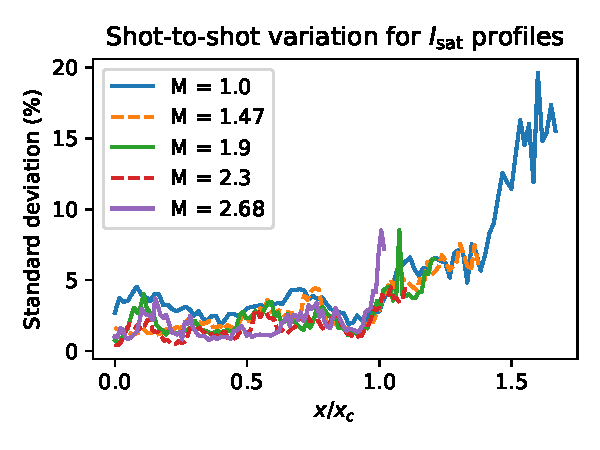
\includegraphics[width=300pt]{figures/extra/isat-profile-stddev.pdf}
    \caption[Shot-to-shot variation of $I_\text{sat}$ profiles]{Shot-to-shot variation of $I_\text{sat}$ profiles}
    \label{fig_extra:isat-profile-stddev}
\end{figure}


Discharge power increases only slightly ($3\%$) at higher mirror ratios suggesting negligible impact on density. Langmuir sweeps and triple probe measurements of $T_e$ (\texttt{DR2}) show slightly (less than 25\%) depressed core and slightly elevated edge $T_e$ with increasing mirror ratio (fig. \ref{fig:Te-sweeps}) but otherwise remains unaffected. The temperature affects $I_\text{sat}$ measurements through the $\sqrt{T_e}$ term so small changes are insignificant. The low temperatures indicate that the plasma is collisional given the length scales of the system (as seen in table \ref{tab:plasma-parameters}) and isotropic. Plasma potential decreases across the plasma (fig. \ref{fig:Vp_ExB}) when the mirror ratio exceeds 1.9. This drop in plasma potential may be caused by the grounding of the anode to the wall, which should begin at $M=1.93$ given the $72$ cm anode and $100$ cm vessel diameters. The reason for the local minimum in the M=2.68 is unknown. This potential profile creates a sheared $\boldsymbol{E \times B}$ velocity profile (fig. \ref{fig:Vp_ExB}) limited to $500$ m/s in the core and exceeding $\sim 3$ km/s at the far edge. The flow does not exceed 4\% of the sound speed (tab. \ref{tab:plasma-parameters}) in the core or gradient ($x=x_{PF}$) region. The mirror ratio does not appear to significantly alter azimuthal flow. The floating potential (Vf) profile also exhibits similar behavior to the plasma potential (fig. \ref{fig:Vp_ExB}), but is modified by the presence of primary electrons. 



\begin{figure}
    \centering
    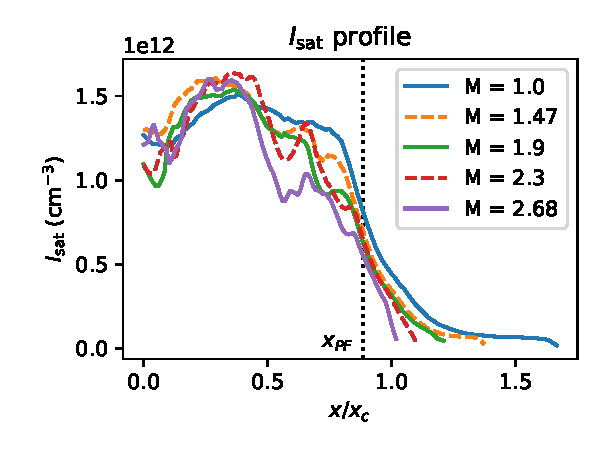
\includegraphics[width=300pt]{figures/fig3.pdf}
    \caption{Midplane $I_\text{sat}$ profile, shot-averaged and time-averaged from 4.8 to 11.2 ms (assumed of $T_e = 4.5$ eV based on triple probe and Langmuir sweep measurements). Effective area was calibrated using a nearby interferometer. Profile shape remains similar in the core and gradient region when mapped to the cathode radius $x_c$. The dips in profiles at higher $M$ below $x=x_\text{PF}$ are of unknown origin and are not the focus of this study. Shot-to-shot variation is less than 5\% for $x \leq 0.95 x_c$ and less than 9\% for $x \leq 1.4 x_c$ for all cases.}
    \label{fig:isat_profile}
\end{figure}

\begin{figure}
    \centering
    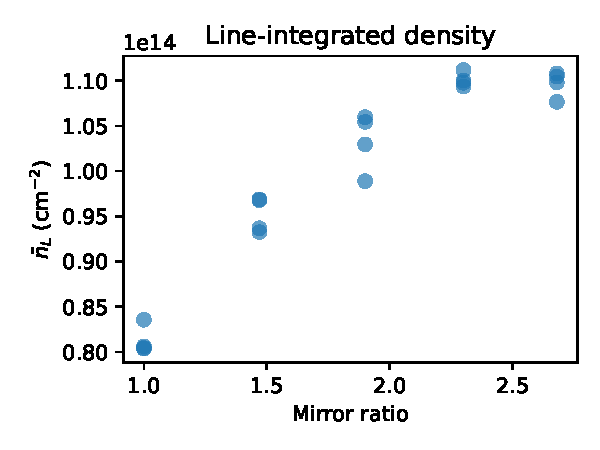
\includegraphics[width=300pt]{figures/fig4.pdf}
    \caption{Line-integrated density as measured by a 56 GHz heterodyne interferometer as a function of mirror ratio, taken from four discharges for each mirror configuration. Density increases up to a mirror ratio of 2.3 where it appears to level off. The interferometer is located in the mirror cell bad-curvature region at 9.59m, 1.3m closer to the cathode from the midplane.}
    \label{fig:density-line}
\end{figure}

\begin{figure}
    \centering
    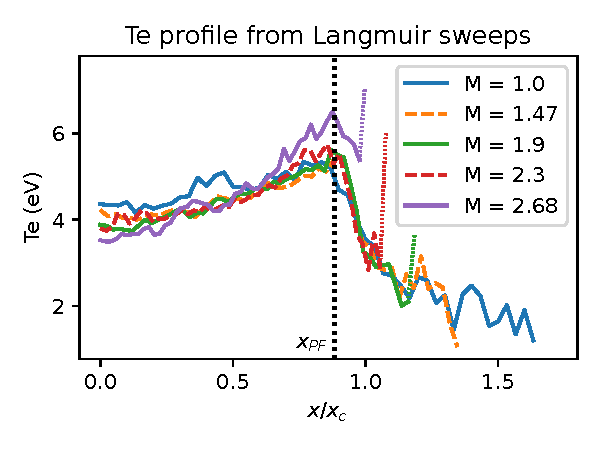
\includegraphics[width=300pt]{figures/fig5.pdf}
    \caption{$T_e$ from Langmuir sweeps (\texttt{DR2}) at the midplane. Triple probe results are nearly identical. The increased temperatures directly at the plasma edge, indicated by dotted portions of the curves, are likely artifacts caused by sheath expansion in lower densities. Changes in mirror ratio lead to at most 25\% change in $T_e$. The plasma is collisional and isotropic.}
    \label{fig:Te-sweeps}
\end{figure}

\begin{figure}
    \centering
    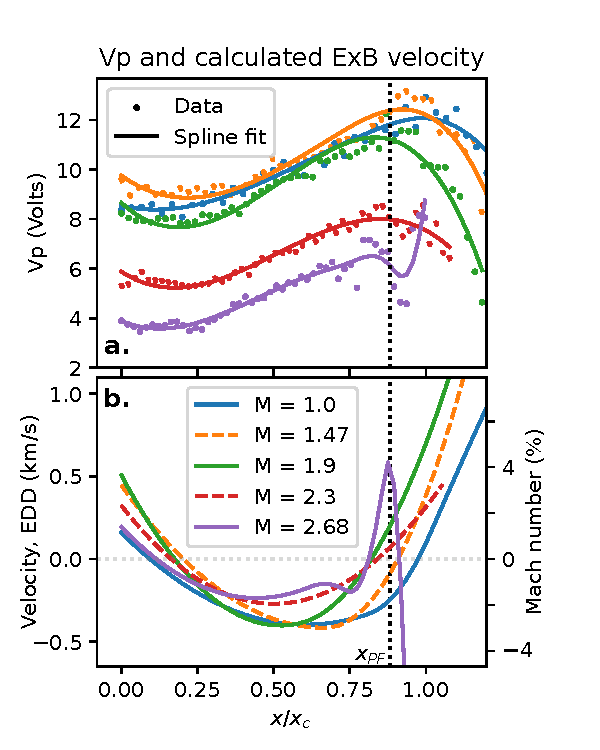
\includegraphics[width=300pt]{figures/fig6.pdf}
    \caption{Plasma potential (a) and derived $\boldsymbol{E \times B}$ velocity profiles (b) from Langmuir sweeps at the midplane. $x/x_c > 1.2$ has been excluded from the graph for greater clarity in the core and gradient region. The electric field was calculated by taking the gradient of the spline-smoothed plasma potential profile. The Mach number (in percent) is calculated using the approximate sound speed evaluated at $x=x_{PF}$ (tab. \ref{tab:plasma-parameters}). The overall structure of the flows does not appreciably change when mirror ratio is varied.}
    \label{fig:Vp_ExB}
\end{figure}

\subsection{Reduced particle flux}

The density fluctuation power peaks at the steepest gradient region ($x_{PF} = x/x_c \sim 0.88)$ as expected as seen in fig. \ref{fig:isat-fluct-prof}. $x_{PF}$ occurs at nearly the same magnetically-mapped coordinate for each mirror ratio. These density fluctuations are a large driver of changes in the cross-field particle flux (eq. \ref{eq:flux}). Vf fluctuations also peak at the same location, but the total power across mirror ratios are similar and, relative to density fluctuations, much lower in the core. Core density fluctuations below 2 kHz are substantial in the core at lower mirror ratios, possibly caused by hollow profiles, nonuniform cathode emissivity, or probe perturbations, but are outside the scope of this study. 
\begin{figure}
    \centering
    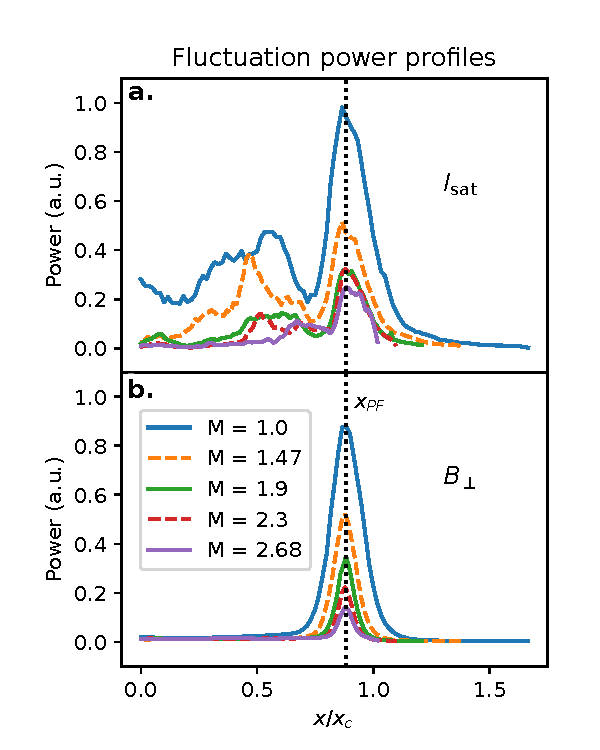
\includegraphics[width=300pt]{figures/fig7.pdf}
    \caption{$I_\text{sat}$ (a) and $B_\perp$ (b) fluctuation power profiles for signals 2 kHz and up at z=8.3m (midplane) and z=7.7m, respectively. The lower frequency components in $I_\text{sat}$ are associated with bulk profile evolution, dominate the core region, and are not the focus of this study.}
    \label{fig:isat-fluct-prof}
\end{figure}

A spectral decomposition technique is used to calculate the time-averaged particle flux \cite{Powers_1974} as seen in fig. \ref{fig:particle-flux}:
\begin{equation}
    \Gamma_{\tilde{E} \times B} = \langle \Tilde{n} \Tilde{v} \rangle = \frac{2}{B} \int^\infty_0 k \left( \omega \right) \gamma_{n \phi} \left( \omega \right) \sin \left( \alpha_{n \phi} \right) \sqrt{ P_{nn} \left( \omega \right) P_{\phi \phi} \left( \omega \right) } d\omega
    \label{eq:flux}
\end{equation}
where $k$ is the azimuthal wavenumber, $\gamma$ is the coherency, $\alpha$ is the cross-phase, and $P$ the power spectrum. This method is more robust than the naive time-integration of $n \left(t \right) \tilde{E} \left( t \right)$ because it accounts for the coherency of the density-potential fluctuations. This representation also enables inspection of each contributing term in the event of surprising or problematic results. A plot of the $I_\text{sat}$-Vf phase can be seen in fig. \ref{fig:isat-Vf_phase}. The flattened particle flux in the core is likely caused by primary electrons emitted by the cathode. These electrons have long mean free paths (greater than a few meters) and sample fluctuations along the length of the machine, mixing the phases of these fluctuations. Since floating potential is set by the hotter electron population, the measured Vf fluctuations are no longer related to the local plasma potential fluctuations of a wave by bulk $T_e$ \cite{Carter_2009}. These primary electrons have a significant effect in the core within the region mapped to the cathode $x \lesssim x_c$. $I_\text{sat}$ fluctuations are not affected.

Azimuthal wave number is measured by two Vf probe tips $0.5$ cm apart. This wavenumber estimation technique yields good agreement with correlation plane measurements (fig. \ref{fig:isat-m-num}). Note that $\tilde{E}$ is not directly measured -- it is instead calculated through the $k(\omega) \sqrt{P_{\phi \phi} (\omega)}$ terms.
The $\tilde{E} \times B$ particle flux clearly decreases with mirror ratio; most of this decrease is attributed to the decrease in density fluctuation power. The particle flux for each mirror ratio was normalized to the $M=1$ case via the plasma circumference to compensate for the increased plasma surface area at the same magnetically-mapped coordinate $x/x_c$. This particle flux is on the order of Bohm diffusion $D_B = \frac{1}{16} \frac{T_e}{B} \approx 6.25 \text{m}^{2} \text{s}^{-1}$ as observed in other transport studies \cite{Maggs-Carter_2008}.
\begin{figure}
    \centering
    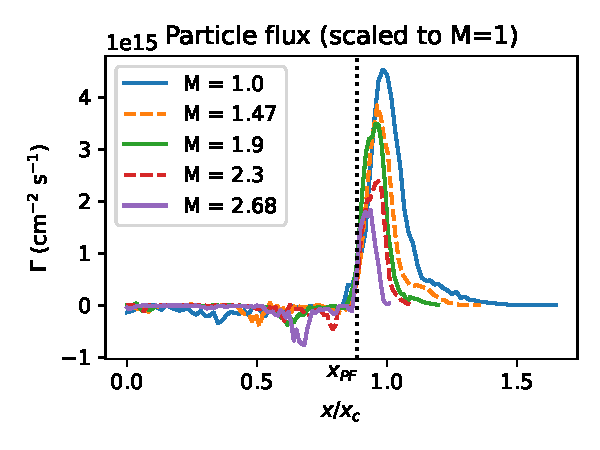
\includegraphics[width=300pt]{figures/fig8.pdf}
    \caption{Cross-field, $\tilde{E} \times B$ fluctuation-based particle flux (calculated using eq. \ref{eq:flux}) with respect to mirror ratio. A monotonic decrease in particle flux is observed with increasing mirror ratio at the midplane. Particle flux is normalized by plasma circumference to the $M=1$ case to account for the geometry-induced decrease in particle flux caused by a larger-diameter plasma.}
    \label{fig:particle-flux}
\end{figure}

\begin{figure}
    \centering
    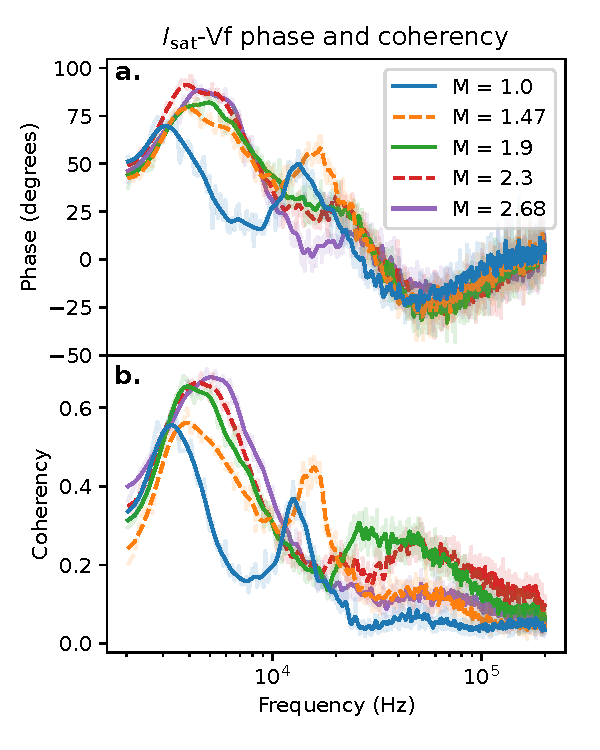
\includegraphics[width=300pt]{figures/fig9.pdf}
    \caption{Phase (a) and coherency (b) of $I_\text{sat}$ current and Vf near $x_{PF}$ at the midplane, smoothed. Positive phase means $I_\text{sat}$ leads Vf. Peaks in coherency occur between 3-5 kHz and at the drift-Alv\'en wave peaks between 12 and 25 kHz. These coherency peaks tend to have larger phase shifts than other nearby frequencies. }
    \label{fig:isat-Vf_phase}
\end{figure}

$T_e$ profiles and fluctuations may affect particle fluxes but measurements of both were not taken in the same datarun; nevertheless, a quantification of the effect of $T_e$ on particle flux is attempted.
$T_e$ fluctuations affect $I_\text{sat}$-based density measurements through the $T_e^{-1/2}$ term, and triple probe and Langmuir sweep $T_e$ measurements suggest that temperature gradients have a negligible impact. A naive incorporation of temperature fluctuation data from \texttt{DR2} into particle fluxes from \texttt{DR1} suggest that cross-field particle flux may be underestimated by up to $50\%$ via the $I_\text{sat}$ temperature term, but the trend and relative fluxes across mirror ratios remain unchanged. Such a naive incorporation should be treated with suspicion because of the sensitive nature of the flux with respect to the gradient and the differences in profiles between \texttt{DR1} and \texttt{DR2}. These difference in profiles made be caused by cathode condition, deposits on the anode, or a different gas mix and are difficult to account for.

\subsection{Compensating for the Te profile}

Electron temperature (Te) compensation for the $I_\text{sat}$ measurement can be done in several ways. One way is to account for the average temperature (i.e., steady state) when calculating the density from $I_\text{sat}$. Te can be gathered from triple probe or swept measurements. Triple probe measurements are generally less reliable than swept probe measurements. The difference between swept and triple probe Te measurements can be seen in fig. \ref{fig:Te_swept_vs_triple}. The two techniques have roughly good agreement, though the triple probe appears to slightly underestimate the temperature. The spikes in the edge are likely from sheath expansion of the probe in the swept measurements (see fig. \ref{fig:Te-sweeps}). 

\begin{figure}
    \centering
    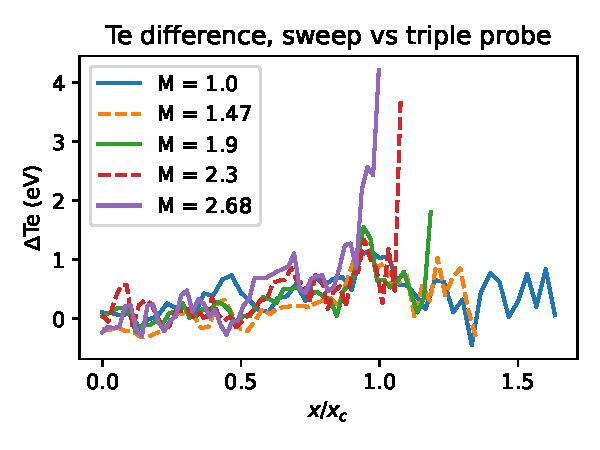
\includegraphics[width=300pt]{figures/Te_sweep-TP_diff.pdf}
    \caption[Swept vs triple probe measurements]{Difference between swept and triple probe temperature measurements. The triple probe appears to slightly underestimate the temperature and temperature gradient. }
    \label{fig:Te_swept_vs_triple}
\end{figure}

Te fluctuations can affect $I_\text{sat}$ fluctuation measurements through the $\sqrt{\text{Te}}$ term. In this case, Te measurements are difficult to compensate for in \texttt{DR1} because of the changes in profiles between \texttt{DR1} and \texttt{DR2}, so the Te fluctuations were included by finding the ratio in \texttt{DR2} of $I_\text{sat}$ fluctuations before and after including these Te fluctuations. This ratio was then applied to \texttt{DR1}. The issue of mismatched profiles still persists but this method allows for changes in fluctuation power between the two datarun sets. In general, $\widetilde{\text{Te}} / \text{Te}$ fluctuations are at most than 30\% (near the edge), and much lower in the core seen in fig. \ref{fig_extra:Te_prof_flucts}. 

\begin{figure}
    \centering
    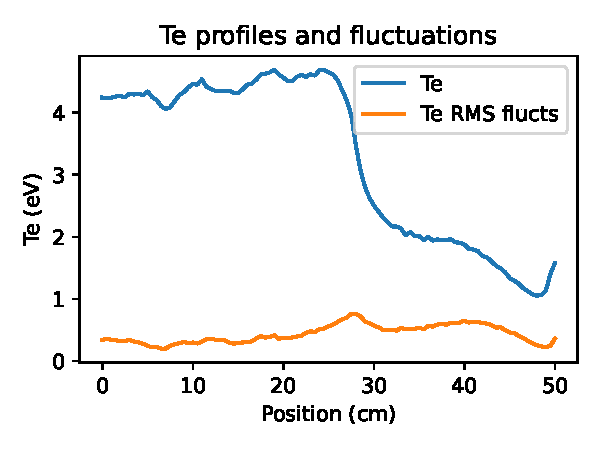
\includegraphics[width=300pt]{figures/extra/Te_prof_flucts.pdf}
    \caption[Triple probe Te and Te fluctuation profiles]{Te and Te fluctuation profiles from the triple probe. RMS electron temperature fluctuations are not particularly large.}
    \label{fig_extra:Te_prof_flucts}
\end{figure}

This Te compensation becomes particularly important when calculating the $I_\text{sat}$ profile gradients which is needed when calculating the diffusivity. A calculation of the diffusivity scaled to the Bohm diffusivity $D_B = \frac{1}{16} \frac{T}{eB}$ can be seen in fig. \ref{fig_extra:diffusivity_tanh}. This calculation uses the particle flux calculated earlier (in the paper) and tanh fit on the density profile for a density smooth gradient. In general, mirror ratios higher than two have a lower diffusivity. When the particle flux is compensated for Te fluctuations, the temperature profile used in for the Bohm diffusion coefficient, and the density profile is smoothed convoluting a $\sigma=2$ cm gaussian, the diffusion coefficient relative to $D_B$ are roughly 2.5 times greater, seen in fig. \ref{fig_extra:diffusivity_Te-comp}. The trend, however, remains relatively the same: higher mirror ratios tend to have a lower diffusivity. The impact of different profile smoothing methods on the density gradient can be seen in fig. \ref{fig_extra:isat_prof_gradient_smoothing}.

\begin{figure}
    \centering
    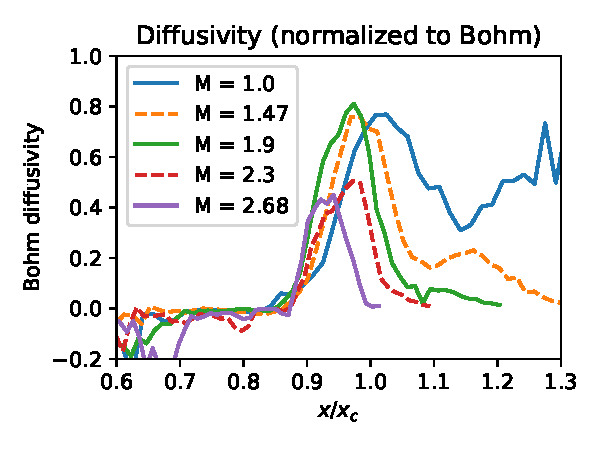
\includegraphics[width=300pt]{figures/extra/diffusivity_tanh-prof-fit.pdf}
    \caption[Diffusivity relative to $D_B$]{Diffusivity relative to $D_B$ using a tanh fit for the density profile and the particle flux measurement assuming a constant Te of 4.5 eV across the profile.}
    \label{fig_extra:diffusivity_tanh}
\end{figure}

\begin{figure}
    \centering
    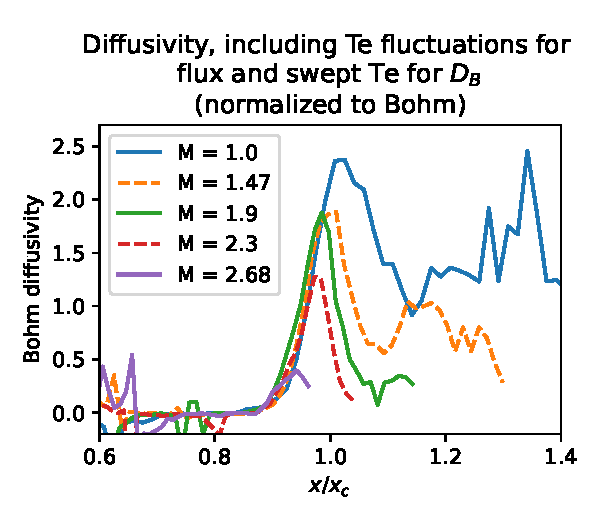
\includegraphics[width=300pt]{figures/extra/diffusivity_Te-comp.pdf}
    \caption[Diffusivity with Te compensation relative to $D_B$]{Diffusivity with Te compensation relative to $D_B$. The particle flux is compensated for Te fluctuations, and the swept-probe temperature profile is used for Te. The diffusivity is around 2.5 times higher than without compensation, but the trend remains similar.}
    \label{fig_extra:diffusivity_Te-comp}
\end{figure}

\begin{figure}
    \centering
    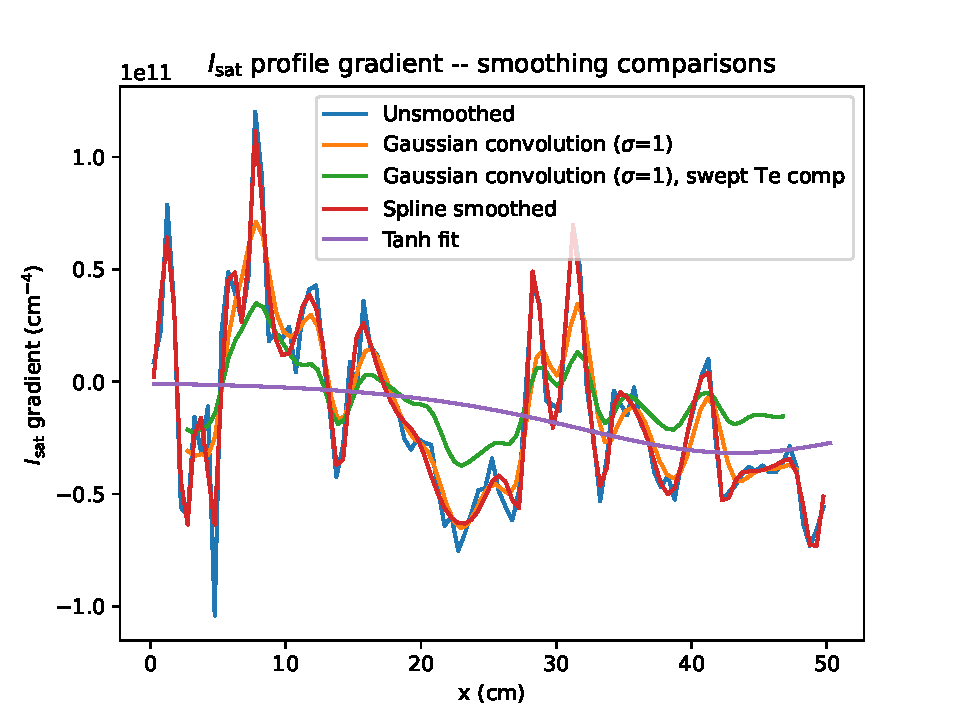
\includegraphics[width=300pt]{figures/extra/isat_prof_gradient_smoothing.pdf}
    \caption[$I_\text{sat}$ gradients under varying profile smoothing methods]{$I_\text{sat}$ gradients under varying profile smoothing methods}
    \label{fig_extra:isat_prof_gradient_smoothing}
\end{figure}

\subsection{Drift waves}
The $I_\text{sat}$ fluctuation power spectra in the region of peak power $x \sim x_\text{PF}$, also where the density gradient is strongest, can be seen in fig. \ref{fig:isat_fluct_power}. Notably, the fluctuation peaks shift to higher frequencies and decrease in total fluctuation power. The shift in frequency may be the Doppler shift caused by the change $\boldsymbol{E \times B}$ plasma rotation seen in fig. \ref{fig:Vp_ExB} at the location $x/x_c \approx x_\text{PF}$. The shift in frequency is somewhat smaller than what would be expected from the field line-averaged increase in Alfv\'en speed at the longest possible wavelength.
\begin{figure}
    \centering
    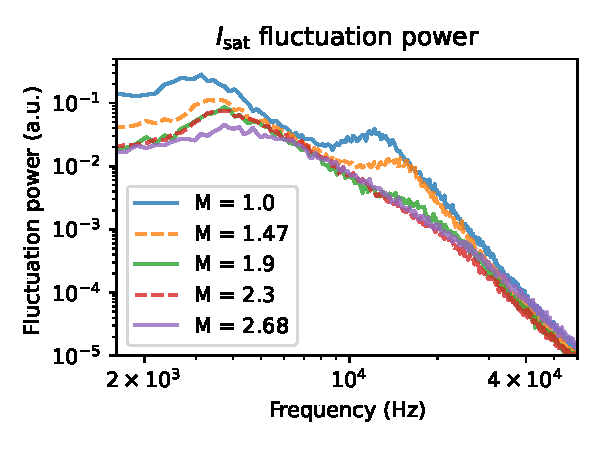
\includegraphics[width=300pt]{figures/fig10.pdf}
    \caption{$I_\text{sat}$ (density) fluctuation power averaged over a 1 cm region around $x_\text{PF}$ at the midplane. The fluctuation power is largely featureless below 2 kHz and beyond 40 kHz aside from electronics noise.}
    \label{fig:isat_fluct_power}
\end{figure}
The phase angle of $I_\text{sat}$ and Vf provides insight into the nature of the driving instability. Including a nonzero resistivity $\eta$ in the drift wave leads to a small phase shift $\delta$ between density and potential.
This phase shift $\delta$ in a collisional plasmas is on the order of $\delta \approx \omega \nu_e / k_\parallel^2 \bar{v}_e^2$ \cite{Horton_1999}. Estimating this quantity using measured and typical values ($k_\parallel = 0.18$ rad/m, $\bar{v}_e = 1300$ km/s, $\nu_e = 3.7$ MHz, $\omega = 12$ kHz) yields a substantial phase shift of $\delta \approx 46^\circ$, which roughly agrees with the phase shifts in fig. \ref{fig:isat-Vf_phase}, though the implied increased phase shift at higher frequencies does not agree with measurements.
As seen in fig. \ref{fig:isat-Vf_phase}, the phase shift between $I_\text{sat}$ and Vf fluctuations are larger below 10 kHz, implying the presence of additional modes beyond or significant modification of resistive drift wave fluctuations.
\begin{figure}
    \centering
    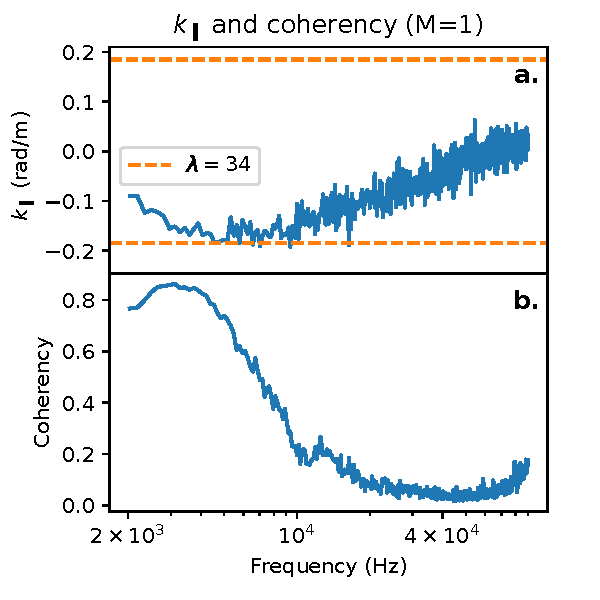
\includegraphics[width=300pt]{figures/fig11.pdf}
    \caption{$k_\parallel$ (a) and coherency $\gamma$ (b) as a function of frequency. Only results from the $M=1$ case are available, but it is clear that there are long ($\gtrsim 34$m) wavelength modes at 3 and 12 kHz. The probes used for calculating $k_\parallel$ were located at the midplane (z=8.31) and z=12.14 m, 3.83 m apart.}
    \label{fig:kparallel-coherency}
\end{figure}
The phase difference between two Vf probes, $3.83$ m apart, was used to calculate the parallel wavelength $\frac{2 \pi}{\lambda} = k_\parallel = \phi_{\text{Vf1, Vf2}} / \Delta z$ assuming the wavelengths are greater than $7.66$ m. The two probes mapped to the same field line only in the $M=1$ configuration, so parallel wavenumbers are available only for the flat case. Parallel wavenumbers are theoretically calculable from 2d correlation planes but the coherency dropped dramatically when a mirror geometry was introduced.
A $34$ m wavelength mode likely contributes to the measured $k_\parallel$ from $3$ to  $\gtrsim 10$ kHz (fig \ref{fig:kparallel-coherency}). Drift waves are long-wavelength modes so coherent density and potential fluctuations along the flux tube are expected. The coherency is a measure of similarity of the spectral content of two signals, in this case Vf probes 1 and 2. The coherency is defined as $\gamma = \frac{|\langle P_{1,2} \rangle|}{\langle |P_{1,1}|^2 \rangle \langle |P_{2,2}|^2 \rangle}$ where $P_{x,y}$ is the cross-spectrum between signals $x$ and $y$ and the angle brackets $\langle \rangle$ denote the mean over shots. The coherency between the two Vf probes drops off with increasing frequency, with a slight bump at around 12 kHz. There are several candidates for the driving mechanism of the 3-5 kHz mode, but the 12 kHz mode is most likely a drift-Alfvén wave.

%\subsection{Drift waves: comparison with theory}
Drift wave theory\cite{Liewer_measurements_1985} suggests that the normalized density fluctuation level $\widetilde n / n$ should fall near 3-10 $\rho_s / L_n$. A plot of this relation using experimental data can be seen in fig. \ref{fig_extra:density-fluct_vs_rhos-Ln}. However, comparison of $\widetilde n / n$ with $1/(k_y L_n)$ show that the normalized density fluctuations are about an order of magnitude too small for the $1/(k_y L_n)$ observed which is unexpected and this conflict has not been able to be resolved in this study. 

\begin{figure}
    \centering
    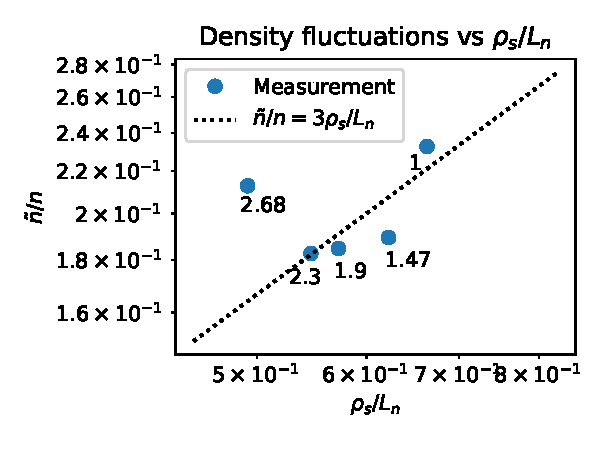
\includegraphics[width=300pt]{figures/extra/density-fluct_vs_rhos-Ln.pdf}
    \caption[Normalized density fluctuations vs $\rho_s / L_n$]{Normalized density fluctuations vs $\rho_s / L_n$. The measured values fall close to the $\tilde{n}/n = 3 \rho_s / L_n$ line which is consistent with theory.}
    \label{fig_extra:density-fluct_vs_rhos-Ln}
\end{figure}

Another issue with this drift-wave interpretation of results is that the electron thermal diffusion along the field line is too high. The plasma must be collisional enough that thermal equilibrium is guaranteed (i.e., the temperature is Maxwellian) , but if the collision rate is too high then thermal gradients can develop along the field line\cite{Goldston_textbook}. This condition on thermal diffusivity condition for the drift wave $\omega$ and $k_z$ is $\omega \ll k_z^2 v_{e, th}^2 / \nu_{ei}$. Plugging in values from the experiments yields frequencies at least 5 times greater than mandated by the diffusivity condition and the condition is violated. This condition violation may be responsible for the odd phase shifts seen between the density and potential fluctuations.

In saturated drift wave turbulence, the normalized density fluctuation amplitude is expected to scale with the gradient scale length $L_n$, so the fluctuation power then scales with $L_n^2$. A plot of this can be seen in fig. \ref{fig_extra:isat_Ln2_n2}. This assumes the same $k_y$, but as mentioned earlier, that scaling and the relationship in general is not consistent with theoretical predictions for saturated drift wave turbulence.

\begin{figure}
	\centering
	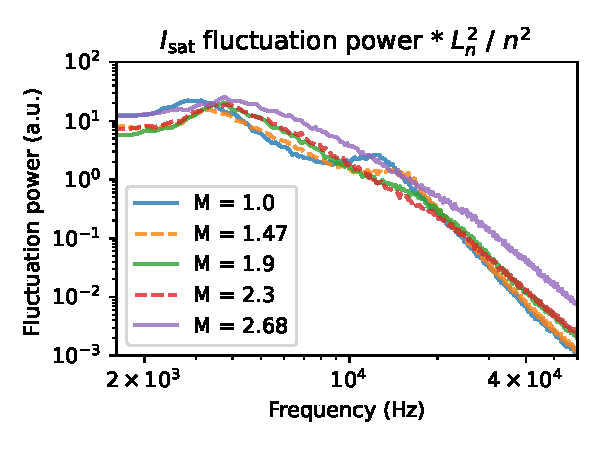
\includegraphics[width=300pt]{figures/extra/isat_fluct_power_Ln2_n2.pdf}
	\caption[$I_\text{sat}$ scaled by $L_n^2 / n^2$]{$I_\text{sat}$ fluctuation power when scaled by the square of the gradient scale length and the squared density. We expect this value to be constant (assuming the same $k_\perp$.}
	\label{fig_extra:isat_Ln2_n2}
\end{figure}


\subsection{\label{sec:sub_turbulence}Turbulence modification}
 The wavenumber-power relation in fig. \ref{fig:fluct-power_ky} shows decreased fluctuation power when a mirror configuration is introduced. However, there is no discernible trend when the mirror ratio is increased further. The exponential nature of the curve also remains unchanged. The greatest decrease in fluctuation power occurred in low and high $k_y$'s, around $10$ and $70$ rad/m. The shape of the power-$k_y$ curves follow an exponential distribution, and is inconsistent with a 2d drift-wave turbulent cascade (Wakatani Hasegawa $k^{-3}$) \cite{Hasegawa-Wakatani}. The steep dropoff in fluctuation power with $k_y$ suggests that higher-wavenumber fluctuations do not have a significant effect on transport.
\begin{figure}
    \centering
    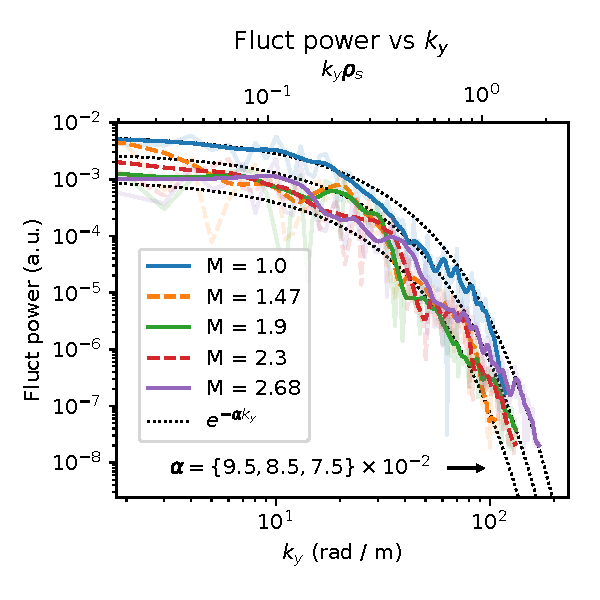
\includegraphics[width=300pt]{figures/fig12.pdf}
    \caption{Fluctuation power summed for each $k_y$ for frequencies up to 100 kHz, smoothed. The contribution to fluctuation power is negligible past 100 kHz. The fluctuation power decreases substantially when a mirror configuration is introduced, but no trend is seen otherwise and the $k_y$ spectra remain exponential. Note the logarithmic scale.}
    \label{fig:fluct-power_ky}
\end{figure}

Previous simulations in a flat field \cite{Friedman_simulation_2013} predicted frequency and wavenumber spectra that can be fit with many power laws or exponentials, but the data presented here (figs. \ref{fig:isat_fluct_power}, \ref{fig:bperp_fluct}, \ref{fig:fluct-power_ky}) appear to follow an exponential relationship within measurement variation.

Turbulence measurements can be directly compared to theoretical predictions and other devices, summarized by Liewer \cite{Liewer_measurements_1985}. For saturated drift wave turbulence, one expects the normalized fluctuation level $\tilde{n}/n \sim 1/\langle k_\perp \rangle L_n$, where $k_\perp$ is some typical wavenumber. The power-weighted $k_y$ (calculated from fig. \ref{fig:fluct-power_ky}) was approximately 15 rad/m, which is an order of magnitude too small to satisfy this relationship. $\tilde{n}/n$ scaling with $\rho_s / L_n$, however, is roughly consistent with drift wave turbulence level saturation: the latter is $\approx 3$ times larger. These comparisons suggest that the large, low frequency fluctuations ($\sim 3$ kHz, which had even smaller $k_y$) may have a drift wave turbulence component but are dominantly driven by other instabilities. No trend is seen in $\rho_s / L_n$ and $1/k_y L_n$ when mirror ratio was varied.

Core fluctuations appear to decrease dramatically as seen in the $I_\text{sat}$ fluctuation power (fig. \ref{fig:isat-fluct-prof}). The $I_\text{sat}$ decorrelation time increases from $\sim0.7$ ms for $M=1$ to $\sim2.5$ ms for $M=2.68$. At $x=x_{PF}$, decorrelation times for all mirror ratios remained at $0.2$ ms.

\subsection{Magnetic fluctuations}
The perpendicular magnetic fluctuation ($B_\perp$) component of the drift-Alfvén wave can be seen in fig. \ref{fig:bperp_fluct}. These $B_\perp$ fluctuations are spatially and spectrally coincident with the electrostatic fluctuations (fig. \ref{fig:isat_fluct_power}).
\begin{figure}
    \centering
    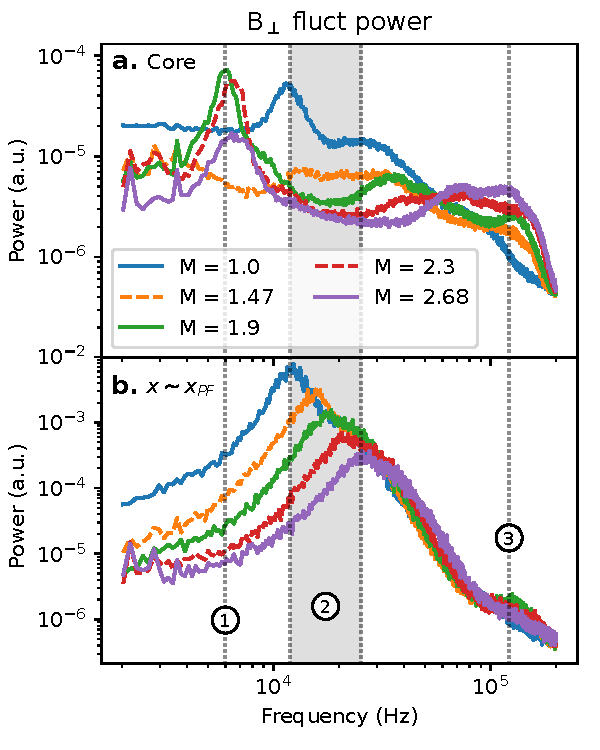
\includegraphics[width=300pt]{figures/fig13.pdf}
    \caption{$B_\perp$ fluctuation power averaged at the core from 0 to 3 cm (a) and around the peak fluctuation point $(x \sim x_{PF})$ (b). Fluctuation power decreases across the board with mirror ratio except for core frequencies close to $\Omega_{ci}$. Peaks around $10-30$ kHz at $x_{PF}$ are consistent (region 2) with drift-Alfvén waves and the near-cyclotron frequency features in the core may be resonating Alfvén waves created by the magnetic mirror. Frequencies below 2 kHz and dominated by instrumentation noise and thus excluded.}
    \label{fig:bperp_fluct}
\end{figure}
Drift-Alfvén waves have been studied in the LAPD in the past \cite{Maggs_1997, Vincena_2006}; strong coupling is observed for $\beta_e > m_e / m_i$ which is satisfied in this study. The Alfvén speed $\omega / k_\parallel = v_A = B/\sqrt{4 \pi n M}$ (given $\omega \ll \Omega_{ci}$) when averaged over the entire column ranges from $\sim 450$ to $\sim 1600$ km/s. A $k_\parallel$ corresponding to a wavelength $\lambda = 34$m roughly falls within the bound established by the kinetic and inertial Alfvén wave dispersion relations at the frequency peaks observed at $x \sim x_{PF}$ seen in fig. \ref{fig:bperp_fluct}. The lengthening of field lines caused by curvature accounts for at most $10\%$ of the change in frequency.

The spatial extent of the $B_\perp$ features identified in fig. \ref{fig:bperp_fluct} are plotted in fig. \ref{fig:Bperp_power_profiles}. Feature 1 at $\approx 6$ kHz shows increased fluctuation amplitudes at $x=0$ for mirror ratios 1.9 and above, but for $M=1$ and $M=1.47$ there is no increase in fluctuation power. A similar feature, but at a much smaller level, is observed in $I_\text{sat}$ fluctuation power in the core as well. This core feature may be caused by the hole in the core seen in the $I_\text{sat}$ profile (fig. \ref{fig:isat_profile}) driving low-amplitude waves or instabilities. Feature 2 in fig. \ref{fig:Bperp_power_profiles} is the magnetic component of the drift-Alfv\'en wave. The fluctuation power peaks at the gradient region and corresponds with the peak in density fluctuations (fig. \ref{fig:isat-fluct-prof}). 

\begin{figure}
    \centering
    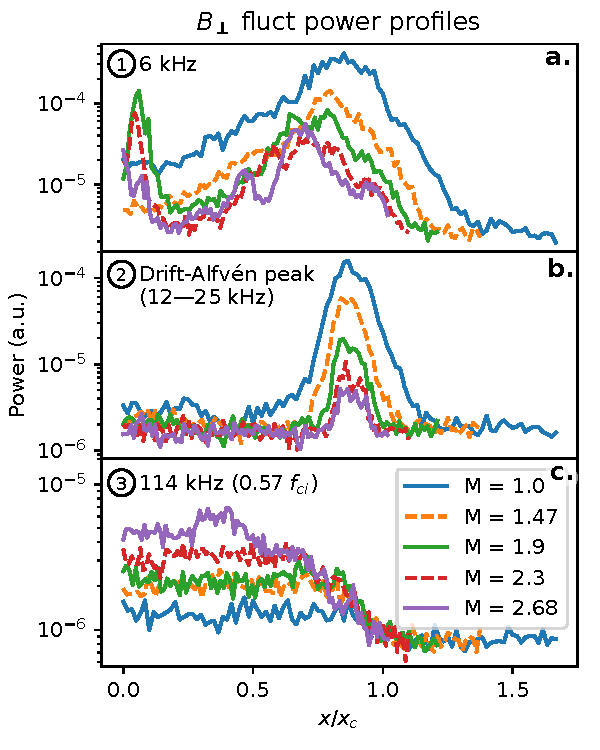
\includegraphics[width=300pt]{figures/fig14.pdf}
    \caption{$B_\perp$ fluctuation power profiles for the three regions shown in fig. \ref{fig:bperp_fluct}: region 1 (6 kHz) (a), region 2 — where frequencies are taken from the peaks of the drift-Alfv\'en waves for each mirror ratio (b), and region 3 (114 kHz) (c).}
    \label{fig:Bperp_power_profiles}
\end{figure}

Feature 3 is particularly interesting because
this the only fluctuating quantity to \textit{increase} with mirror ratio, seen in fig. \ref{fig:Bperp_core_highfreq}. This feature may be broad evanescent Alfv\'enic fluctuations from the plasma source.
These fluctuations have been observed in the LAPD in the source region alongside an Alfvén wave maser \cite{Maggs_2005}. Note that the Alfv\'en maser cannot enter the mirror cell at mirror ratios greater than 1.75 because the Alfv\'en maser resonates at 0.57 $f_{ci}$ but the midplane is always at or near 500G. 

\begin{figure}
    \centering
    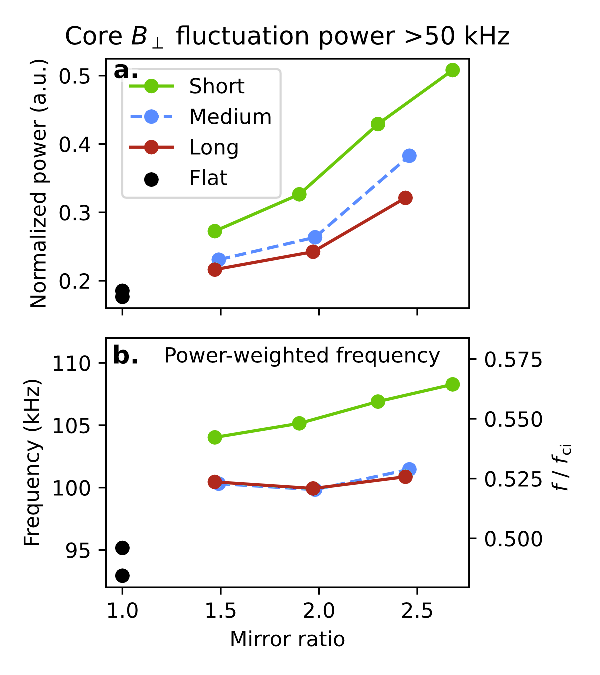
\includegraphics[width=300pt]{figures/fig15.pdf}
    \caption{Summed fluctuation power of $B_\perp$ in the core ($x/x_c \leq 0.3$) as a function of mirror length and ratio. Top (a): the fluctuation power is normalized by the sum of the full-spectrum summed power. Bottom(b): the frequency of the power distribution > 50 kHz weighted by the fluctuation power.}
    \label{fig:Bperp_core_highfreq}
\end{figure}

The sub-$2$ kHz modes in $B_\perp$ and its harmonics are nearly constant in power across the entire plasma; these features are likely perturbations from the magnet power supplies and thus ignored. The lack of radial, azimuthal, and axial structure in these magnetic signals below 2 kHz and narrow bandwidth indicate a non-plasma origin. Significant radial and azimuthal structure in $B_\perp$ fluctuation power starts to appear in frequencies larger than 4 kHz.

%\subsection{Additional Bdot analysis}
The drift-Alfv\'enic nature of the 12 kHz Bdot feature is confirmed by changing the flat field from 500G to 400G: the feature shifts down in frequency from 12 to 10 kHz seen in fig. \ref{fig_extra:bperp_500G-vs-400G}. From the drift wave and Alfv\'en wave dispersion relations the frequency is expected to be 400G / 500G $= 0.8$ of the original, which is approximately what is observed. The $k_y$ of the drift-Alfv\'en wave also has an effect and may be responsible for a 10 kHz / 12 kHz $= 0.83$ factor instead. 
\begin{figure}
    \centering
    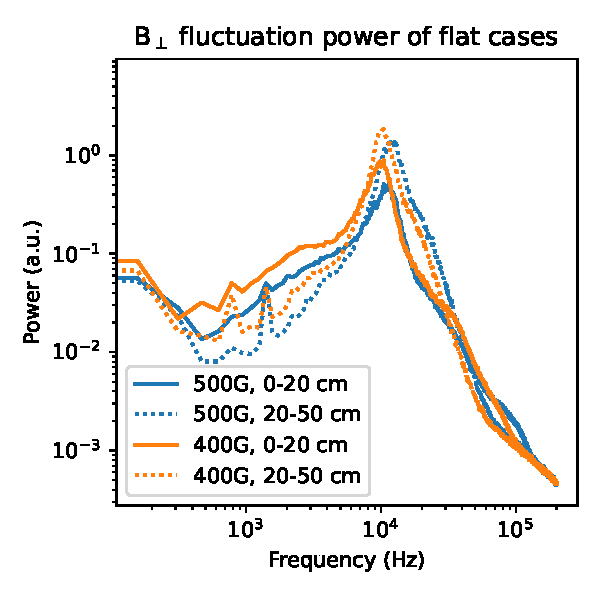
\includegraphics[width=250pt]{figures/extra/Bperp_fluct_power_M=1_400G_500G.pdf}
    \caption[$B_\perp$, flat field 500G vs 400G]{$B_\perp$ flat field for 500G and 400G flat fields. The frequency of the identified drift-Alfv\'en wave at 12 kHz drops when the field is lowered, as expected.}
    \label{fig_extra:bperp_500G-vs-400G}
\end{figure}

There may be some sort of resonator made by the mirror cell and its interaction with Alfv\'en waves. In fig. \ref{fig_extra:Bperp_power_core_lengths}, the behavior of the $B_\perp$ spectrum in the core changes dramatically between 1 and 10 kHz in the short mirror when compared with the medium and longer mirrors. It's unlikely that this is an Alfv\'enic fluctuation because the wavelength is an order of magnitude too large to fit in the machine. 

\begin{figure}
    \centering
    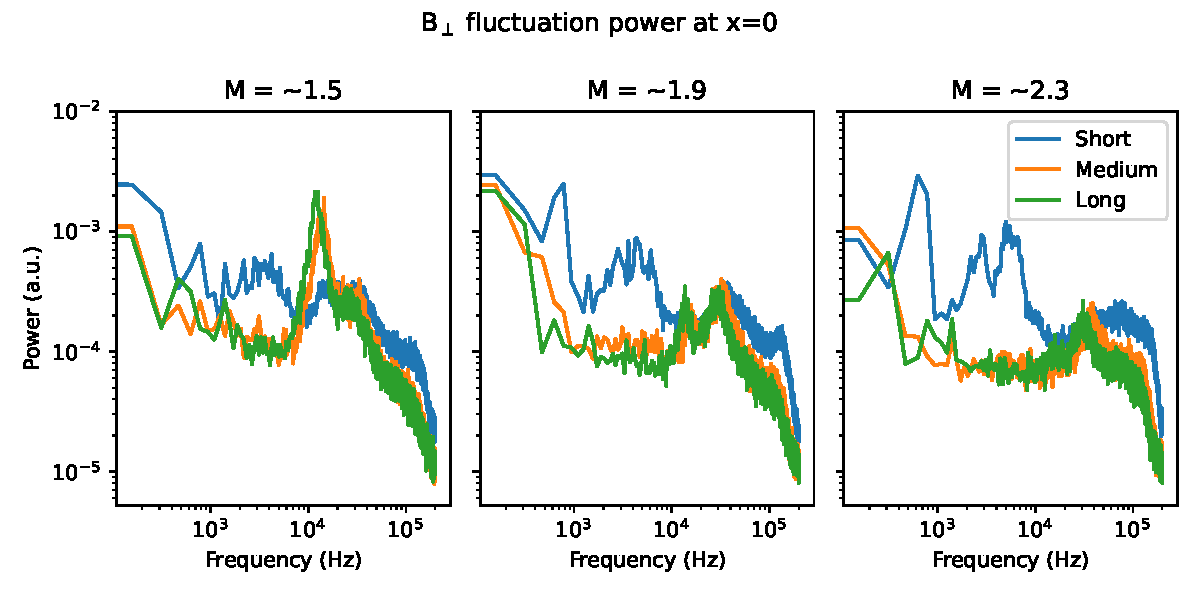
\includegraphics[width=400pt]{figures/extra/Bperp_power_core_lengths.pdf}
    \caption[$B_\perp$ fluctuations at x=0 for different mirror lengths]{$B_\perp$ at x=0 for different mirror lengths. The origin of fluctuations between 1 and 10 kHz is unknown.}
    \label{fig_extra:Bperp_power_core_lengths}
\end{figure}

For completeness, $B_z$ fluctuation measurements are seen in fig. \ref{fig_extra:Bz}. The peaks in the 10 kHz region are likely crosstalk or slight coil misalignment of the probe and are picking up $B_\perp$ fluctuations. The profile low frequency $B_z$ fluctuations can be seen 

\begin{figure}
    \centering
    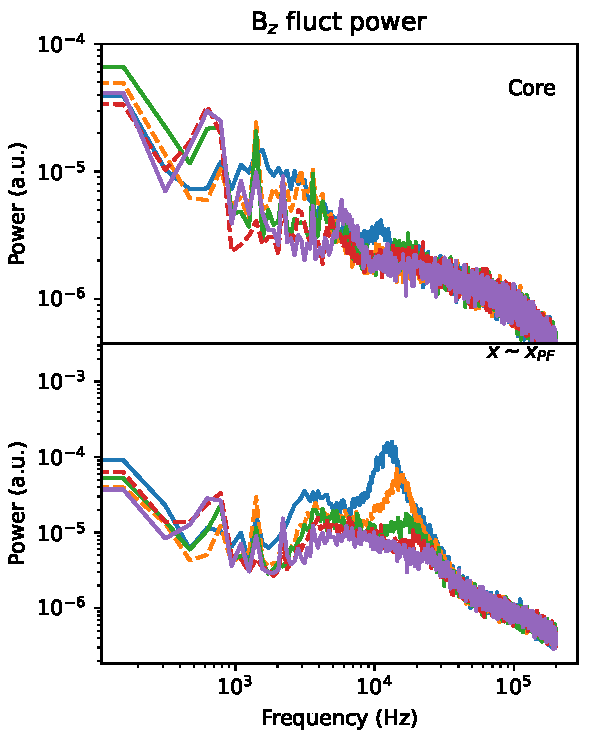
\includegraphics[width=300pt]{figures/extra/Bz_fluct_power_core_edge.pdf}
    \caption[$B_z$ fluctuations in the core and $x_{PF}$]{$B_z$ fluctuations in the core and $x_{PF}$. Aside from picking up some $B_\perp$ signal, the spectra are largely featureless.}
    \label{fig_extra:Bz}
\end{figure}

The low frequency fluctuations in the Bdot spectra may seem important but plotting the spectra as a function of position (fig. \ref{fig_extra:Bperp_lowfreq_profile}) clearly shows the harmonics of the signal and the narrow bandwidth of them. This spectral feature is present regardless of mirror ratio, but changes in magnitude in approximate proportion with the field, i.e., the magnet power supply current. This power supply-induced field fluctuation can easily be seen in the $\approx 625$ Hz mode in $B_z$, seen in fig. \ref{fig:B_z_625Hz}. The fluctuation power is largely constant across the entire plasma column, with the fluctuation power increasing with increased mirror fields. The taper of the fluctuation power at the edge could be caused by the background field vector no longer pointing in the $z$ direction as the probe approaches the magnet coil. In general, the probe valves are not centered between the magnet coils, leading to rotation of the of the field vector as the probe is pulled out.

\begin{figure}
    \centering
    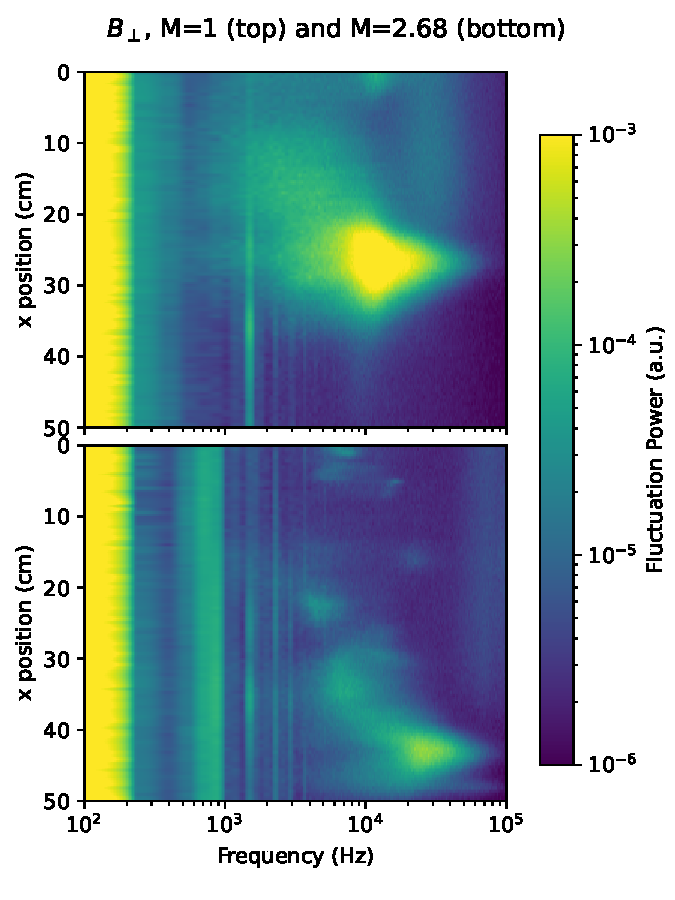
\includegraphics[width=300pt]{figures/extra/bperp_x-vs-f_lowfreq_M=1_and_2-68}
    \caption[$B_\perp$ fluctuation power profiles for low frequencies]{$B_\perp$ fluctuation power for mirror ratios of 1 and 2.68. Lower frequencies are shown and the colorbar clipped to show detail in what appears to be power supply fluctuations}
    \label{fig_extra:Bperp_lowfreq_profile}
\end{figure}

\begin{figure}
    \centering
    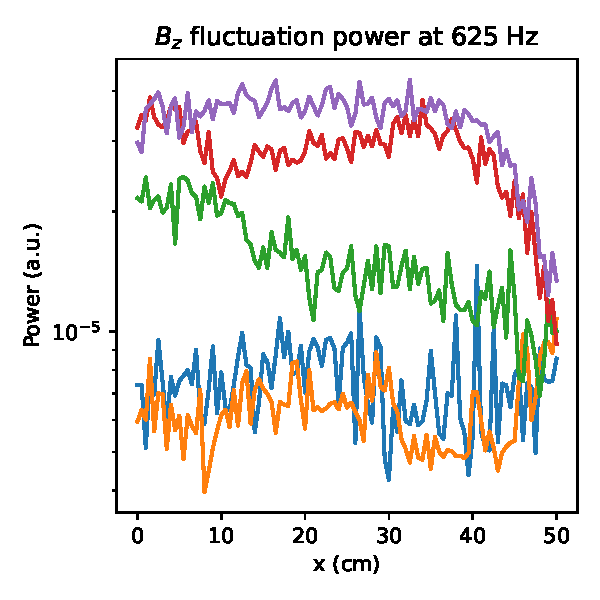
\includegraphics[width=300pt]{figures/Bz-fluct-profile_625-Hz}
    \caption[$B_z$ fluctuation power profiles for low frequencies]{$B_z$ fluctuation power profiles for all mirror ratios at 625 Hz. }
    \label{fig:B_z_625Hz}
\end{figure}

\section{\label{sec:structure}2d Structure}
The perpendicular magnetic field structure is measured by collecting x-y planar bdot ($d B_{\{x, y, z \} } / dt$) data alongside a stationary, axially separated $I_\text{sat}$ reference probe (\texttt{DR2}). This probe provides a phase reference for the magnetic field fluctuations, allowing a 2d map of relative phase to be constructed over many shots. Only the region around $x_{PF}$ was measured because of constraints on probe movement. The amplitude and phases for each magnetic field component are then used to reconstruct the local magnetic fluctuation vector $\boldsymbol{B}$. The axial current density structure, $j_z$, can be derived from this vector field. $\boldsymbol{B}$ and the corresponding $j_z$ for the flat-field ($M=1$) case can be seen in fig. \ref{fig:Bvec_jz_M=1}.
Two main current channels can be seen with the magnetic fields circulating around them. This structure quickly decoheres in time as expected in a turbulent plasma. At higher mirror ratios, the field magnitude and corresponding current density decrease (which was also seen in \texttt{DR1}: fig. \ref{fig:bperp_fluct}). Similar structure is seen in the mirror configurations; the $M=1.9$ and $M=2.68$ cases can be seen in fig. \ref{fig:Bvec_jz_M=1-9+2-68}. 
\begin{figure}
    \centering
    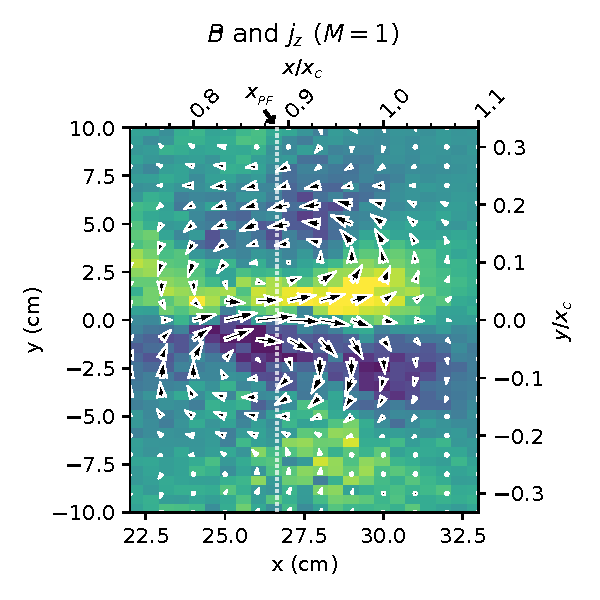
\includegraphics[width=300pt]{figures/fig16.pdf}
    \caption{Perpendicular magnetic field and the derived current density for the flat-field ($M=1$) case using a Bdot probe with an axially-separated $I_\text{sat}$ reference (\texttt{DR2}). The x-y plane was centered near $x_{PF}$.}
    \label{fig:Bvec_jz_M=1}
\end{figure}

\begin{figure}
    \centering
    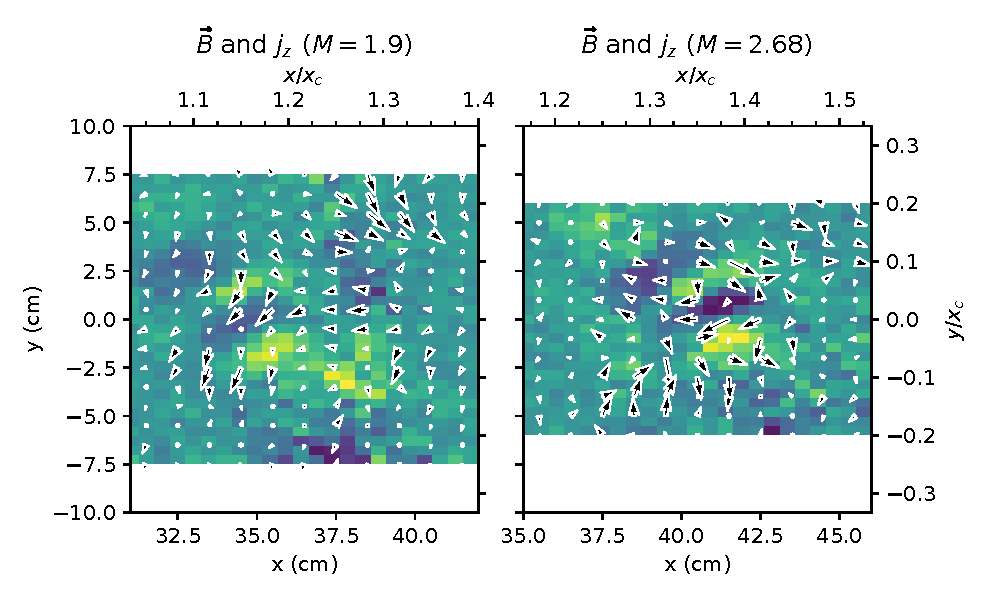
\includegraphics[width=450pt]{figures/Bvec_Jz_M=1-9+2-68.pdf}
    \caption{Perpendicular magnetic field and the derived current density for the $M=1.9$ and $M=2.68$ cases computed in the same manner as fig. \ref{fig:Bvec_jz_M=1}. The x-y planes were centered near $x_{PF}$, and the view size was kept constant across the plots. The structure is much less obvious in the mirror cases, but all exhibit the expected Alfv\`en wave pattern}. 
    \label{fig:Bvec_jz_M=1-9+2-68}
\end{figure}

Using two, axially-separated, correlated $I_\text{sat}$ measurements (\texttt{DR2}), with one collecting x-y planar data, the azimuthal mode number $m$ (radially integrated) was calculated. Higher-frequency and higher-$m$ features are seen with increasing mirror ratio (fig. \ref{fig:isat-m-num}). The increased frequencies may be caused by a  change in Doppler shift by the $\boldsymbol{E \times B}$ flow. This higher-m trend suggests that azimuthal structures do not scale with increased plasma radius but instead remain roughly the same size. The limited planar probe movement caused an increase in the lower bound on $m$  in higher mirror ratios. At mirror ratios 1.47 and higher, the lower frequency component ($< 10$ kHz) appears to decrease significantly in amplitude. 
\begin{figure}
    \centering
    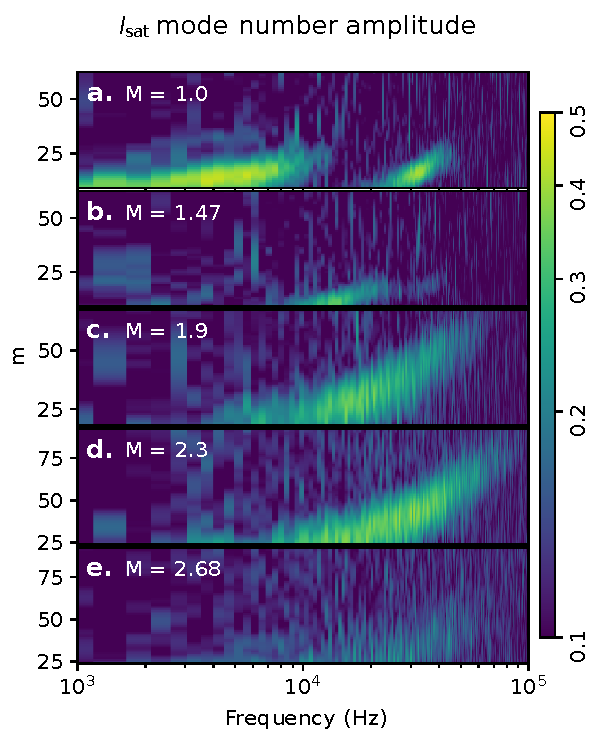
\includegraphics[width=300pt]{figures/fig17.pdf}
    \caption{Azimuthal mode number $m$ amplitudes calculated from two axially-separated, correlated, $I_\text{sat}$ probes. Increasing mirror ratio (a to e) leads to increased $m$ at higher frequencies. (\texttt{DR2})}
    \label{fig:isat-m-num}
\end{figure}
Calculating $k_\perp$ from $m$ evaluated at $x \sim x_c$ yields similar $k_y$ values as the two-tip technique (fig. \ref{fig:kperp}). The average $k_y$ for a given frequency can be calculated using two Vf tips on the same probe by calculating the phase difference and dividing by the spatial separation of $5$ mm: $k_y = \phi_{\text{vf1, vf2}} / \Delta y$ \cite{Powers-twoprobe-ky}. The maximum $|k_y|$ measurable before aliasing is $\pi / \Delta y \approx 628$ rad/m. As seen in fig. \ref{fig:kperp}, the $k_y$ spectrum remains similar across mirror ratios, but the wavenumber extends further into higher frequencies with increasing mirror ratio. 
\begin{figure}
    \centering
    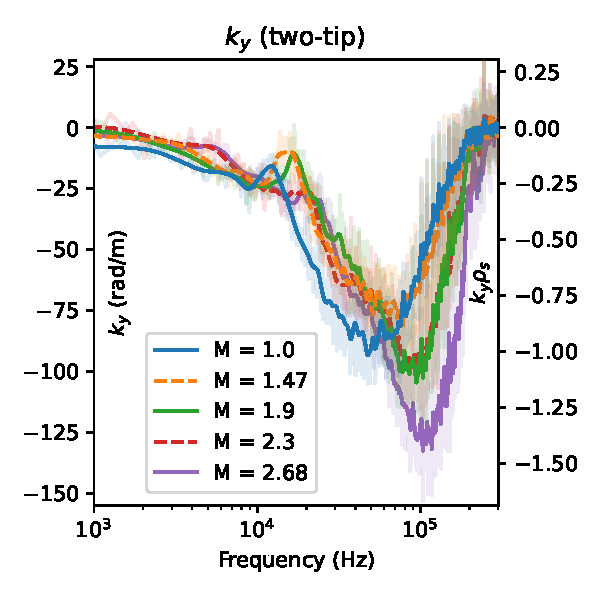
\includegraphics[width=300pt]{figures/fig18.pdf}
    \caption{$k_y$ averaged about $x_{PF}$ and smoothed for each mirror ratio calculated using two vertically-separated Vf tips on the same probe. Little change is seen in $k_y$ at lower frequencies but higher frequencies tend towards larger $k_y$ at higher mirror ratios.}
    \label{fig:kperp}
\end{figure}
These azimuthal mode numbers and gradient scale lengths are consistent with linear simulations using the 3d fluid code \texttt{BOUT} \cite{Popovich_2010} in the flat, unbiased case.

\section{\label{sec:discussion}Discussion}
\subsection{Lack of mirror-driven instabilities}
No evidence is seen for mirror-driven instabilities — curvature, loss-cone, or otherwise. Given the LAPD parameters in this study (tables \ref{tab:fields} and \ref{tab:plasma-parameters}), the collision frequencies are sufficiently high such that the mirror is in the gas-dynamic regime: losses out of the mirror throat are governed by gas-dynamic equations rather than free streaming through the loss cone. To be in the gas-dynamic regime, the mirror length must exceed the mean free path of the ions \cite{Ivanov_2013}:
\begin{equation}
    L > \lambda_{ii} \ln{M} / M
\end{equation}
where $L$ is the mirror length, $\lambda_{ii}$ is the ion mean free path, and $M$ is the mirror ratio.
These collisions populate the loss cone and maintain a (cold) Maxwellian distribution, eliminating the possibility of loss-cone-, ion-driven instabilities like the AIC \cite{Casper_1982} or DCLC \cite{Simonen_1976,Kanaev_1979} instabilities that have been observed in other (historic) devices. 

The paraxial, approximate interchange growth rate is \cite{Post_1987,Ryutov_2011}
\begin{equation}
    \Gamma_0 = \frac{c_s}{\sqrt{L_M L_P}}
\end{equation}
which yields $\Gamma_0 \approx 1.2$ kHz using $L_M \approx 7$m and $L_P = 17$m. $c_s$ is used instead of $\bar{v_i}$ because $T_i \ll T_e$ and mirror length $L$ is split to distinguish between the contributions of the plasma length and mirror length to inertia and to curvature drive, respectively.
Interchange is not visible in-part because the aspect ratio of these mirrors is quite large, limiting the growth rate of interchange. The length of the mirror (3.5 m), radius of curvature (6-7 m), and plasma column (17 m) are much larger than the radius of the plasma (0.5 m maximum), so the plasma inertia is large relative to the instability drivers. Line-tying to the cathode may further lower the growth rate. The hot cathode used for plasma formation could function as a thermionic endplate that can supply current to short out the flute-like interchange perturbations. Line-tying has been seen in flux rope experiments on the LAPD using a hotter, denser source \cite{Compernolle_2011}, also in other devices \cite{Fornaca_1979}, and is why interchange was not seen in the earliest mirror machines \cite{Post_1987}. Note that the plasma terminates on the cathode or end plates before the magnetic field flares out, so there is no contribution to stability from an expander tank as seen in other GDTs \cite{Ryutov_2011,Ivanov_2013}. 
Finite Larmor radius (FLR) effects may provide a stabilizing effect for larger azimuthal mode numbers. 
At the highest mirror ratio, assuming a plasma radius of $a_0 =\sqrt{2.68} * x_{PF}=43$ cm, the FLR stability criterion $\frac{m}{2} \frac{\rho_i L}{a_0^2} > 1$ \cite{Ryutov_2011} suggests a stabilizing effect may be present for azimuthal mode numbers $m > 4$.

If the curvature-induced interchange instability were observable, then introducing a mirror configuration would lead to new features in $I_\text{sat}$ and Bdot fluctuations. In particular, low-frequency mode(s)  -- likely less than 10 kHz given the low m-number and plasma rotation rates -- would be observed growing from the pressure gradient region. For onset of the interchange instability, the mirror curvature or plasma pressure would need to be increased but the precise conditions required for this onset are not yet known for the LAPD.

Interchange could also be at least partially stabilized by the continuous production of electrons in the core that are electrostatically trapped by the ambipolar potential \cite{Guest_1971}. The intuition behind this stabilization mechanism is as follows: electrons are continuously produced via ionization of neutrals, and any change in the local potential will cause more or fewer electrons to be lost out the ends of the device along that field line, counteracting the potential change. This stabilization mechanism has been experimentally demonstrated  to completely suppress interchange when the ambipolar potential $\Phi \gtrsim 6T_e$ \cite{Komori_1987}.

The $\boldsymbol{E \times B}$ shear flow present (fig. \ref{fig:Vp_ExB}) may also make a contribution to the stabilization of interchange \cite{Ryutov_2011,Bagryansky_2003,Bagryansky_2007,Beklemishev_2010}. The estimated shearing rate is between 3 and 10 kHz, which is greater than the estimated $\approx 1.2$ kHz growth rate of the interchange mode.

\subsection{Instabilities driving LAPD turbulence}

Rotational interchange can be significant driver of the broadband turbulence spectrum in the LAPD, particularly when a biased limiter is installed. This observation has been confirmed by both linear simulations \cite{Popovich_2010} and biasing experiments \cite{Schaffner_2013}. 

This rotational interchange mode has the following attributes, as summarized by \cite{Jassby_transverse_1972}: flute-like ($k_\parallel=0)$, $|e\tilde{\phi}/T_e|/|\tilde{n}/n| \gtrsim 1$, radial potential phase variation $45$ to $90^\circ$, maximum possible $|e\tilde{\phi}/T_e| < 1$. All of these attributes are seen for the lower frequency (3 kHz) mode. The Vf radial phase variation when $M>1$ is not clearly seen because the coherency is dramatically reduced along the field line.
The rotational interchange mode could couple with the drift wave at $k_\parallel = \pi / L \sim 0.37$ rad/m ($n=0.5$), which has been observed in the past \cite{Schaffner_2013} and likely present here.
Estimates of shearing rate from the $\boldsymbol{E \times B}$ flow velocity profile (fig. \ref{fig:Vp_ExB}), calculated fluctuation ratios, and radial phase shift variation suggest that Kelvin-Helmholtz-driven turbulence is not significant, if present at all. Historically, biasing a limiter has been required to clearly observe the Kelvin-Helmholtz instability \cite{horton_vorticity_2005, Schaffner_2012, Schaffner_2013}.

Low frequency density fluctuations may also be driven by a flute-like conducting-wall temperature-gradient instability which only requires an electron temperature gradient to grow (even with straight field lines) \cite{Berk_1991}. Simulations of turbulence in the LAPD suggest the possible presence of these conducting wall modes (CWM) which have the highest growth rate for $m \leq 20$ \cite{Friedman_2013}. This lower-$m$ mode could be responsible for the peak around $3$ kHz in the $M=1$ $I_\text{sat}$ fluctuation (fig. \ref{fig:isat_fluct_power}) and azimuthal mode numbers (fig. \ref{fig:isat-m-num}) and for the low-frequency low-$k_\parallel$ or flute-like behavior (fig. \ref{fig:kparallel-coherency}). This CWM may also be responsible for flatter electron temperature profiles seen in previous studies \cite{Perks_impact_2022, Schaffner_2013} (fig. \ref{fig:Te-sweeps}). 

These linearly unstable modes may be outgrown by a rapidly-growing nonlinear instability that couples to drift-like modes as suggested by simulations \cite{Friedman_2013}. This nonlinear instability is driven by the density gradient at an axial modenumber of $n=0$ and nonlinearly transfers energy to $n \neq 0$ fluctuations. 

The conducting wall mode and nonlinear instability may be present in these mirror experiments but the spectra are adequately explained by linearly unstable modes. Precise identification these modes requires further study; neither of these instabilities have been directly observed in the LAPD.

\subsection{Causes of particle flux reduction}

\begin{figure}
    \centering
    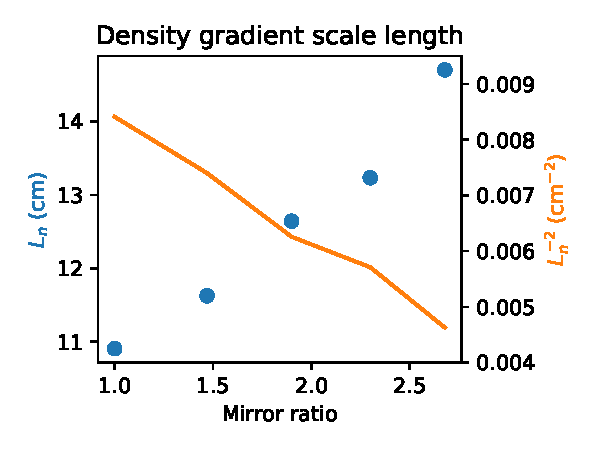
\includegraphics[width=300pt]{figures/fig19.pdf}
    \caption{Gradient scale length $L_n$ and the associated term in the drift wave growth rate $L_n^{-2}$. This scale length was calculated over a 3 cm region around $x_\text{PF}$ (peak fluctuation region) at the midplane. Increasing the mirror ratio increases the gradient scale length, which suggests weakening of the underlying instability driver.}
    \label{fig:L_n}
\end{figure}

The reduction in particle flux explained by a reduction in density fluctuations likely caused by a increased gradient scale length $L_n = \frac{n}{\nabla n }$ (fig. \ref{fig:L_n}), decreasing the linear drift wave growth rate and saturation level seen in sec. \ref{sec:sub_turbulence}. This gradient length reduction may also reduce the growth rate of the rotational interchange instability, which may be the dominate driver for the low-frequency large-amplitude density fluctuations. The influence of this density fluctuation reduction appears reduced at higher mirror ratios past $M=1.9$, where the wavenumber and phase angle appear to decrease in magnitude. The plot showing this breakdown in particle flux can be seen in fig. \ref{fig_extra:particle_flux_breakdown}. The changes in $I_\text{sat}$ fluctuation power is the most obvious driver, but the $I_\text{sat}$ - Vf phase difference, coherency and wavenumber also seem to have an effect. The Vf fluctuation power remains largely consistent across the different mirror ratios. Note that this particle flux appears somewhat different because this is using the uncalibrated $I_\text{sat}$ values and the flux is not scaled by solid angle. This flux also does not use temperature-compensated $I_\text{sat}$ measurements.

\begin{figure}
    \centering
    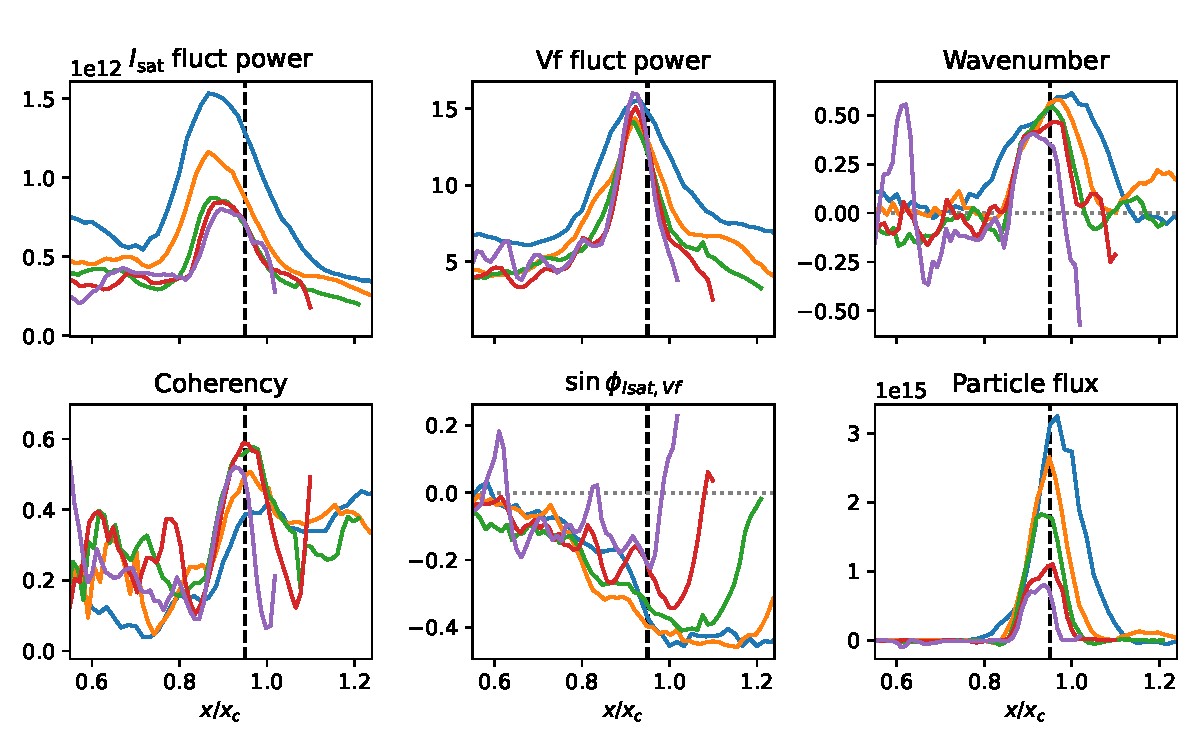
\includegraphics[width=450pt]{figures/extra/particle_flux_breakdown.pdf}
    \caption[Particle flux: breakdown into components]{The particle flux broken down into the components used to calculate it. The dashed black line is simply a visual reference near the peak particle flux at $x/x_c=0.95$. The $I_\text{sat}$ fluctuation power appears to be the largest driver in changes in particle flux. The colored lines correspond to mirror ratio as seen in earlier plots.}
    \label{fig_extra:particle_flux_breakdown}
\end{figure}

The decorrelation time of $I_\text{sat}$ time series data is around 0.15 ms at $x_\text{PF}$. An estimate of the $\boldsymbol{E \times B}$ flow shear from fig. \ref{fig:Vp_ExB} (\texttt{DR2}) yields a shearing time between 0.1 and 0.3 ms at $x_\text{PF}$. These times suggest that spontaneous flow shear may be important for suppressing turbulence, as seen in other studies \cite{Schaffner_turbulence_2013,Cho_2005}, at all mirror ratios. However, no clear trend in shearing strength is seen with mirror ratio.

The decorrelation time of a signal is calculated by taking the autocorrelation of a signal -- $I_\text{sat}$ in this case -- and finding the full-width half-max of the envelope using a Hilbert transform. This decorrelation time can be seen in fig. \ref{fig_extra:decorrelation_time}. The decorrelation is minimized  at $x_{PF}$ and maximized in the core, further confirming the turbulent nature of the fluctuations at $x_{PF}$.
\begin{figure}
    \centering
    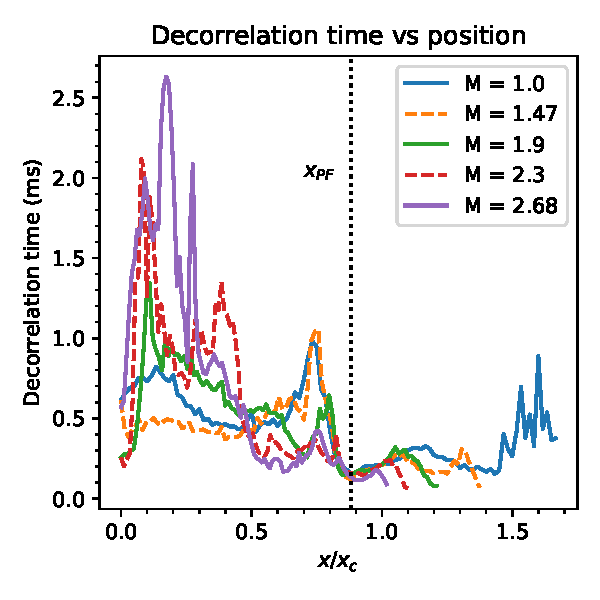
\includegraphics[width=300pt]{figures/extra/decorrelation_time.pdf}
    \caption[$I_\text{sat}$ decorrelation time]{Decorrelation time from $I_\text{sat}$ time series data for different mirror ratios. All of the mirror ratios have a minimum decorrelation time at $x_{PF}$ and much longer times (slower rate) in the core.}
    \label{fig_extra:decorrelation_time}
\end{figure}

The estimated shearing rate from \texttt{DR2} can be seen in fig. \ref{fig_extra:ExB_shearing-rate}. The rate is plotted instead of time because of the singularity when the flow reverses. At around $x_{PF}$ ($x/x_c \approx 0.87$), the shearing rate is around 2 to 8 kHz meaning the shearing time is around 0.5 to 0.125 ms. This is fairly close to the decorrelation time from the $I_\text{sat}$ time series measurements (fig. \ref{fig_extra:decorrelation_time}). These similar times/rates suggests that ExB shearing may set the limit on cross-field transport.

\begin{figure}
    \centering
    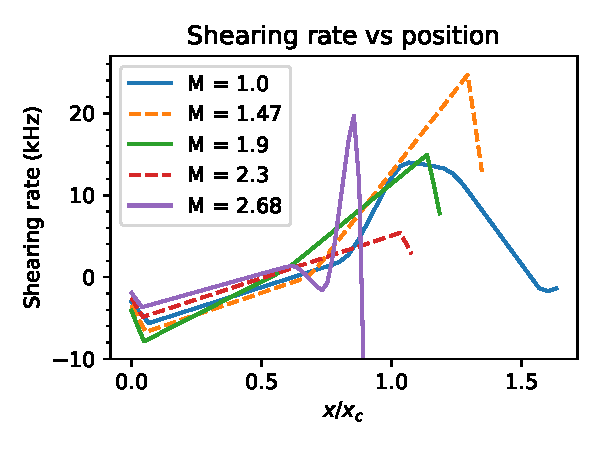
\includegraphics[width=300pt]{figures/extra/ExB_shearing-rate_zoomed.pdf}
    \caption[ExB shearing rate]{ExB shearing rate.}
    \label{fig_extra:ExB_shearing-rate}
\end{figure}


It is important to note that the electron thermal diffusion time along the field line is very long compared to the frequency of the drift wave ($\omega \gtrsim k_\parallel \bar{v}_e^2 / \nu_{ei}$) \cite{Goldston_textbook} so the electron temperature along the field line may not be constant on the drift wave timescale. This factor is not taken into account in this analysis but may have substantial impact on interpretations of the measured phase shift.

\subsection{Differences between \texttt{DR1} and \texttt{DR2}}
Directly applying signals between these two dataruns is not quite appropriate because the profiles/plasmas changed appreciably. These changes could have been caused by differences in cathode temperature, emissivity, or other properties. The discharge power for \texttt{DR2} was roughly 10\% smaller than what was seen in \texttt{DR2} seen in fig. \ref{fig_extra:discharger-power_vs_M}. Since the discharge voltages were similar (\texttt{DR1}: 62.5 vs \texttt{DR2}: 60.5) we expect to see less dense plasmas in \texttt{DR2}. 
\begin{figure}
    \centering
    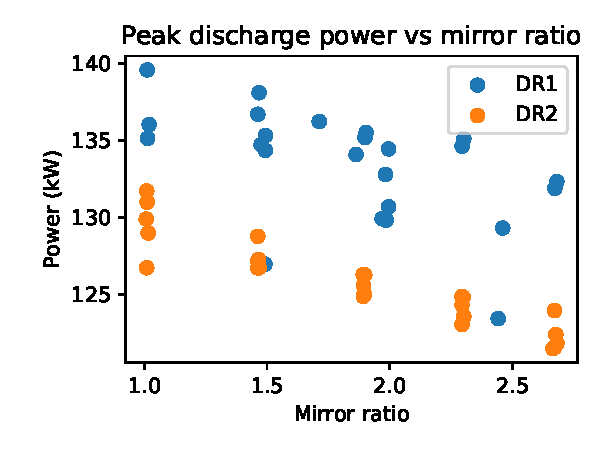
\includegraphics[width=300pt]{figures/extra/discharge-power_vs_M.pdf}
    \caption[Discharge power vs mirror ratio]{}
    \label{fig_extra:discharger-power_vs_M}
\end{figure}

Changes in the $I_\text{sat}$ profiles between the two dataruns (and between two separate measurements in \texttt{DR1}) can be seen in fig. \ref{fig_extra:DR1-DR2_isat_profile_comparison}. Interestingly, there is some difference in the profiles \emph{within the same datarun} which could be caused by probe shadowing. Probe shadowing effects should be less important in mirrors because the probe closest to the cathode magnetically maps to a region further outside than the probes in the mirror cell. This difference in density can also be seen in the line-integrated density from the 56 GHz interferometer (port 23): fig. \ref{fig_extra:M_vs_nbar}. These differences in density could also be caused by different hydrogen and helium pressures in the runs. Helium pressure was roughly the same for both dataruns (6e-6 to 3e-6 for \texttt{DR1}, 6e-6 to 2e-5 for \texttt{DR2}), but the hydrogen pressure was an order of magnitude higher for the \texttt{DR2}, on the order 7e-6 instead of 1e-7 for \texttt{DR1}. These differences in pressures could have had an effect on plasma formation and transport, thus affecting profiles. Hydrogen fraction is known to have an effect on breakdown characteristics in the newer Lanthanum-hexaboride (LaB6) cathode.
\begin{figure}
    \centering
    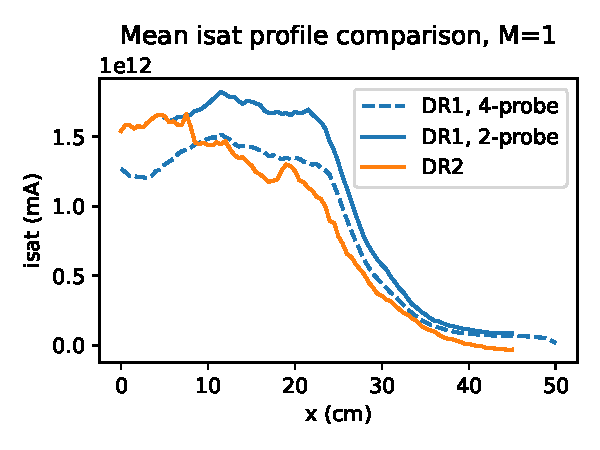
\includegraphics[width=300pt]{figures/extra/isat_profile_comparison.pdf}
    \caption[$I_\text{sat}$ profiles (M=1), \texttt{DR1} vs \texttt{DR2}]{$I_\text{sat}$ profiles (M=1), \texttt{DR1} vs \texttt{DR2} in the mirror cell.}
    \label{fig_extra:DR1-DR2_isat_profile_comparison}
\end{figure}

\begin{figure}
    \centering
    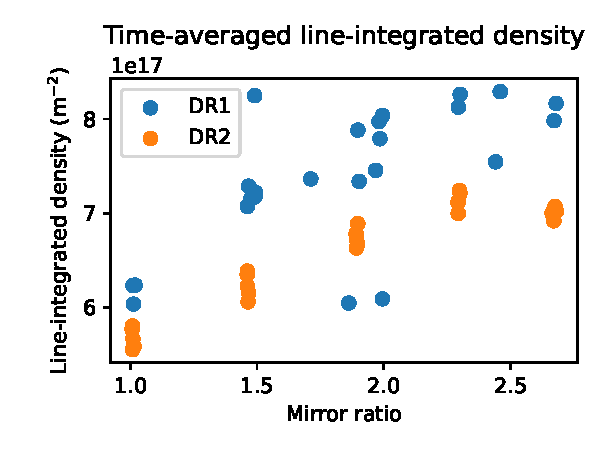
\includegraphics[width=300pt]{figures/extra/M_vs_nbar.pdf}
    \caption[Line integrated density, \texttt{DR1} vs \texttt{DR2}]{Line integrated density from the 56 GHz, \texttt{DR1} vs \texttt{DR2}. On average, \texttt{DR2} has a lower density than what's seen in \texttt{DR1}. The interferometer is located near the region of good curvature closest to the cathode.}
    \label{fig_extra:M_vs_nbar}
\end{figure}

Differences could also occur within dataruns. Calibrating the effective area of the $I_\text{sat}$ probes can be done using the 56 GHz interferometer, but this calibration factor drifted over time and seen in fig. \ref{fig_extra:isat_calibration_factor}. This could be deposits being removed or added to the probe, affecting the effective area. This calls into question the reliability of absolute $I_\text{sat}$ measurements, but we proceed regardless because there's no easy way to fix this issue. 

\begin{figure}
    \centering
    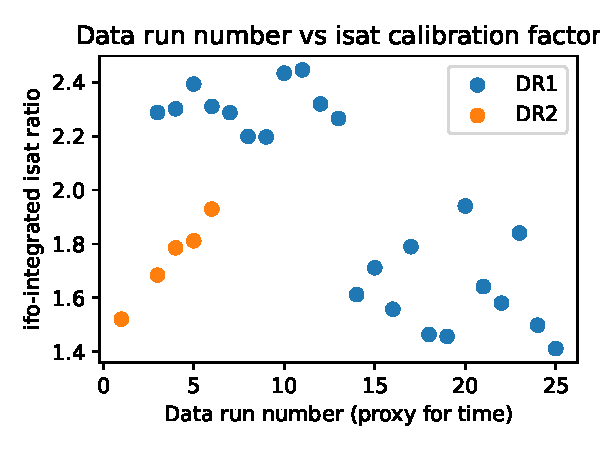
\includegraphics[width=300pt]{figures/extra/run-num_vs_nbar-isat-ratio.pdf}
    \caption[$I_\text{sat}$ calibration factor over runs]{$I_\text{sat}$ calibration factor over different dataruns from the same run sets. Datarun number is monotonically increasing, so in this case it's used as a proxy for time. A rather large variance is seen in this calibration factor, which suggests the $I_\text{sat}$ probes having time-varying characteristics affecting the measurement.}
    \label{fig_extra:isat_calibration_factor}
\end{figure}


\section{\label{sec:conclusion}Conclusions and future work}

Turbulence and transport was studied in mirrors with varying lengths and ratios using the flexible magnetic geometry of the LAPD. Particle flux and fluctuation amplitudes decreased up to a factor of two when mirror ratio was increased. The primary drivers of turbulence were identified as the rotational interchange mode, caused by spontaneous rotation, and unstable drift-Alfvén waves driven by the density gradient. The decrease in density fluctuation amplitudes can be attributed to an increase in the gradient scale length caused by the dimensionally wider plasma at the mirror midplane. Despite imposing a mirror configuration, no signs of mirror-driven instabilities were observed. The highly-collisional, GDT-like plasma produced suppressed any velocity space instabilities. The interchange growth rate was likely suppressed to an undetectable level by line-tying, in-cell electron production, and shear flow.

Future experiments in hotter regimes with the new LaB6 cathode \cite{LAPD_LaB6} will need to be performed to evaluate the robustness of these results, particularly concerning the stabilization of curvature-induced interchange. Additionally, the source field should be matched to the mirror midplane field so that the plasma remains the same radius to isolate geometric effects.
Simultaneous measurements using flux and/or vorticity probes and $I_\text{sat}$ are needed to concretely determine if azimuthal flow shear is modified by the mirror field, and to quantify the effect of flows on rotational interchange and drift wave instability drive in general.
Multiple simultaneous axial measurements of potential would enable better understanding of the axial wavenumber and identification of possible modes.

%This work was performed at the Basic Plasma Science Facility, which is a DOE Office of Science, FES collaborative user facility and is funded by DOE (DE-FC02-07ER54918) and the National Science Foundation (NSF-PHY 1036140). The authors would like to thank Dr. Giovanni Rossi and Dr. Steven Vincena for probe setup and assistance with data collection, and Dr. Mel Abler, Prof. Walter Gekelman, and Prof. George Morales for insightful discussion.
%
%The data and code supporting this study are available from the corresponding author upon reasonable request.
%
%Competing interests: The author(s) declare none.


%\section{Bibliography}
%\bibliographystyle{jpp}
%\bibliography{_bibliography}









































\graphicspath{{Chapters/Chapter_ml-dataruns/}}

\chapter{Creating a randomized  dataset for machine learning tasks}
\label{ch:ml-dataruns}

\section{Goal and introduction}

The goal of collecting this dataset was to maximize the diversity of data coming from the LAPD. Previous datasets -- even one made of 29 million passively-collected shots over three years -- did not contain sufficient diversity to do an interesting ML study. In particular, the data must be sufficiently diverse to allow an optimization study without the need to collect more data. In addition, many diagnostics were recorded so that the signals could be correlated on the same shot, either in the machine learning model itself or as a preprocessing step. This chapter describes the process of collecting this data, example signals, and biases within the dataset. All of the data from this campaign (several terabytes) is available upon request. 

The LAPD has many experimental control parameters for various physics studies. While the device can accommodate various insertable components, this dataset focuses on the parameters fundamental to the operation of the main cathode. Specifically, half way between the cathode and anode are three gas puff valves: East, West, and top. The aperture, duration, and triggering of these valves has a large impact on plasma formation. A static gas fill system also exists but it is not used. The cathode-anode voltage (and consequently, discharge power) strongly influences plasma density and temperature downstream of the source. Additionally, the magnetic field configuration substantially shapes the plasma column. One crucial variable not considered in this dataset is the cathode temperature, as its adjustment and equilibration requires many hours, limiting dataset diversity. This combination of diagnostic coverage, high repetition rate, and extensive configurability renders the LAPD particularly suitable for machine learning studies. 

\section{Configuration of the LAPD}

Data collection was conducted in two campaigns separated by 14 months. The initial run set is designated as \texttt{DR1} and the subsequent run set as \texttt{DR2}. These run sets are further broken down into \em dataruns \em which are series of discharges (``shots'') with identical operational machine parameters. A total of 67 dataruns were collected over both campaigns. These two datarun sets had significant intrinsic differences: \texttt{DR1} had two turbomolecular pumps offline, leading to much higher background pressures. In addition, the cathode condition in terms of emissivity or asymmetries is unquantified, so there may be intrinsic differences in the plasma produced regardless of machine configuration. 

The LAPD control parameters varied in this dataset were the source field, mirror field, midplane field, gas puff valve voltage, gas puff duration, and discharge voltage. The magnetic field regions are labeled in fig. \ref{fig:ml-lapd-diagnostics} and effectively control the width of the plasma relative to the cathode in their respective regions. The gas puff voltage governs gas flow rate into the chamber, though this relationship is not yet quantified, and the gas puff duration defines the piezo valve activation period. For \texttt{DR1}, the discharge voltage is applied across the cathode and anode at the same time as the gas puff, but for \texttt{DR2} applied 10 ms after gas puff initiation. This difference between runs was not known at experiment time. While discharge voltage correlates to discharge current (and thus power), the current depends on the machine configuration and downstream conditions and cannot be predetermined.

These machine parameters -- with the exception of gas puff duration -- were randomly sampled via Latin-hypercube sampling (LHS) for 44 of the dataruns. LHS is a pseudorandom sampler that guarantees that each machine setting is set at least once. An example of LHS vs random sampling can be seen in fig. \ref{fig:lhs-vs-random}. It is possible for random sampling to miss certain machine settings, or entire portions of configuration space altogether. This fact is particularly important when the number of samples is small, such as in this case with 44 samples. Data were then collected with these settings. Gas puff duration was reduced for the last seven runs to 20, 10, or 5 ms (see fig. \ref{fig:PP1_time-series-example} for timings relative to $I_\text{sat}$ signals). The breakdown of each setting in the dataset is given in appendix \ref{sec:app_bias}, Table \ref{tab:data_frac}. The top gas puff valve was used for only the first nine dataruns of \texttt{DR2} because of equipment issues. 23 of the dataruns in the dataset are not random: they were chosen to be similar to common machine configurations used in more conventional studies, usually using flat fields (or different cathode fields) around 1 kG. These data were taken while other diagnostics were being configured.

\begin{figure}
	\centering
	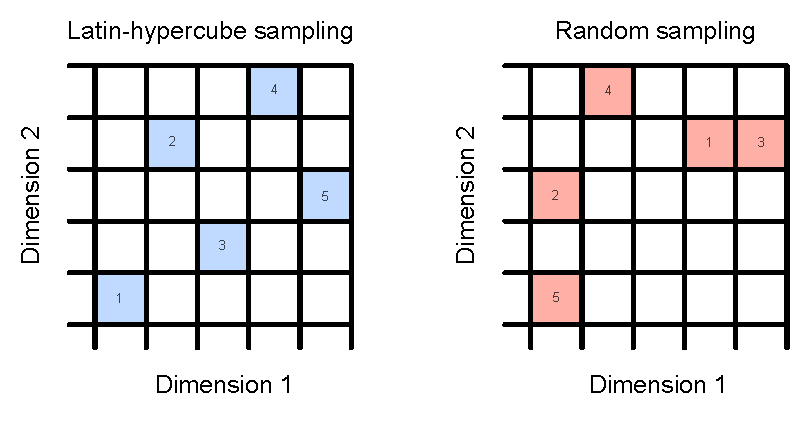
\includegraphics[width=350pt]{figures/lhs.pdf}
	\caption[A demonstration of Latin-hypercube sampling vs random sampling]{\label{fig:lhs-vs-random}An example of Latin Hypercube Sampling compared to a potential random sample of five points. LHS hits all rows and columns, but random sampling may leave some sections of parameter unsampled space altogether.}
\end{figure}

$I_\text{sat}$ and other probe-based measurements were acquired along y=0 lines (51 dataruns total) or x-y grids (16 dataruns total) with spatial resolutions varying between 1.5 to 2 cm. The fixed axial locations of the probes were 895 cm and 831 in \texttt{DR1} and 1150, 1022, 863, and 639 cm for \texttt{DR2} (Fig. \ref{fig:LAPD_coords}). Six shots were recorded at each position except for the first four dataruns in \texttt{DR1} with five shots each.

\section{Signals collected}

\texttt{DR1} and \texttt{DR2} had considerable overlap in diagnostics recorded, with some minor difference. A summary of the diagnostics and their locations on the LAPD can be seen in fig. \ref{fig:ml-lapd-diagnostics}. Some of the raw diagnostics signals and machine state information (MSI) can be seen in fig. \ref{fig:example-diagnostics-msi}. Some dataruns may not contain all diagnostics, as some data were collected while other diagnostics were being set up. The diagnostics and machine state information (MSI) recorded for this dataset are the following:
\begin{itemize}
	\item \textbf{\texttt{DR1} probes}: three probes were inserted into the LAPD. One had Langmuir sweeps, another "flux probe" had $I_\text{sat}$ and two floating potential (V$_\text{f}$) tips, and the last "triple probe" had $I_\text{sat}$, V$_\text{f}$ and electron temperature ($T_e$). These signals were digitized at 6.25 MHz (100 MHz, 16 sample average).
	\item \textbf{\texttt{DR2} probes}: four probes were inserted, namely a flux probe, triple probe, Langmuir sweeps with $I_\text{sat}$ on a separate tip, and another flux probe. These signals were digitized at 6.25 MHz (100 MHz, 16 sample average).
	\item \textbf{Diodes}: five diodes, axially distributed, were recorded as well. The one closest to the cathode had a He-II line filter. The diodes were uncalibrated, have a nonlinear response, and are sensitive beyond the visible spectrum. These diodes were a part of the MSI system and were recorded at 25 kHz. Each diode (besides the one with the He-II filter) had 8 layers of 1-stop (50\% transmission) neutral density filter in front of the diode.
	\item \textbf{Interferometer}: signals from the 288 GHz heterodyne interferometer was recorded on an oscilloscope at 10 MHz, which was then downsampled to 100 kHz before analysis so that the processing computer could keep pace.
	\item \textbf{Thomson scattering}: a single point was measured on-axis at port 32, triggered at 8 ms into the plasma for \texttt{DR1} or 12 ms for \texttt{DR2}. Periodically the collection optics were scanned to maximize the light collected. during both run set.
	\item \textbf{Spectrometer}: an ocean optics HR4000 spectrometer recorded spectra integrated over the duration of the shot. The spectrometer has a very narrow slit, leading to good spectral resolution but requiring many shots for a clean spectrum.
	\item \textbf{Monochromator (\texttt{DR2} only}): three Helium neutral lines were recorded, namely 587, 667, and 707 nm, using an oscilloscope sampling at 1 MHz.
	\item \textbf{Diamagnetic loop}: the loop sits between ports 34 and 35 and consists of one large loop and two smaller concentric loops equaling the area of the large one. These signals were digitized using an oscilloscope at 500 kHz, but are strongly influenced by magnet power supply noise making analysis difficult.
	\item \textbf{Fast framing camera}: a Phantom v7.3 fast framing camera recorded plasma dynamics from the end of the machine, pointing towards the cathode. The images are monochrome, 14 bit, 14 $\mu$s exposure, $256\times256$ pixels, and 2,500 fps using a 105 mm lens. The camera is capable of 36,697 fps at that resolution, but a lower one was used to lessen file transfer times and storage requirements.
	\item \textbf{Discharge current and voltage}: as part of the MSI system, time evolution of the discharge current and voltage are recorded at 25 kHz.
	\item \textbf{Magnetic field profiles}: theoretical on-axis magnetic field values are calculated using the magnet power supplies. Both are recorded as part of the MSI. For the work here, we simply use the programmed field values for the cathode, mirror, and midplane regions. Occasionally the calculated field would be incorrect since the power supply currents for the cathode are set manually, which is the case in some dataruns here, but the profiles is unused in these studies so it isn't an issue.
	\item \textbf{Pressures}: total pressure and pressure breakdown by atomic mass unit are recorded by an ion gauge and RGA, respectively. The RGA takes around a couple minutes to complete a scan but the data should be reasonably accurate given the slow time-evolution of pressure.
\end{itemize}

\begin{figure}
	\centering
	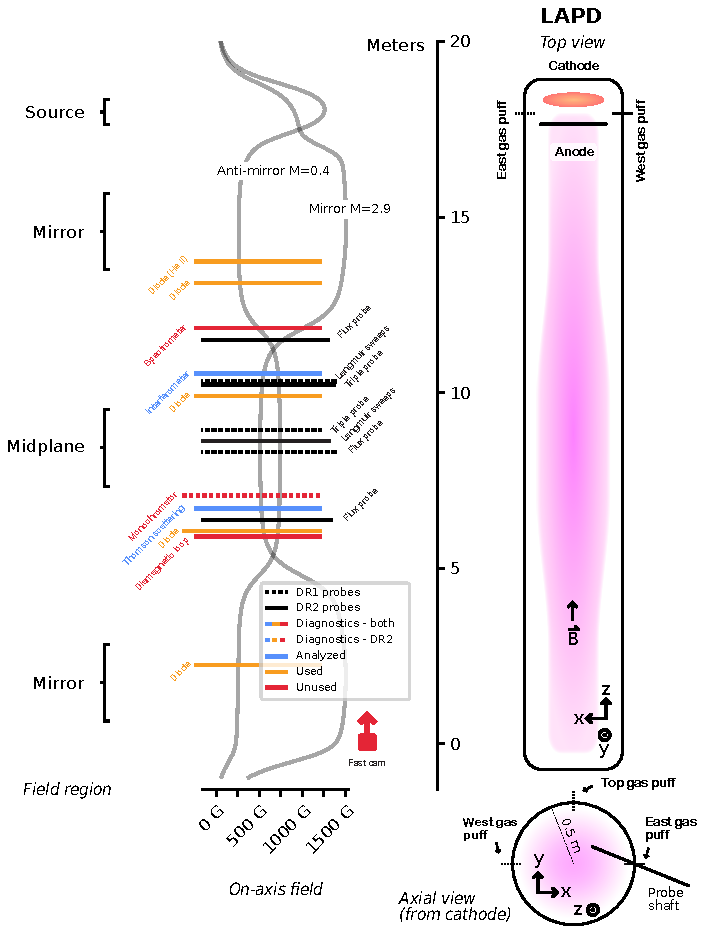
\includegraphics[width=440pt]{figures/lapd-diagnostics.pdf}
	\caption[LAPD configuration and diagnostics for the ML datarun]{\label{fig:ml-lapd-diagnostics}Diagnostics and example field configurations for \texttt{DR1} and \texttt{DR2}}
\end{figure}

\begin{figure}
	\centering
	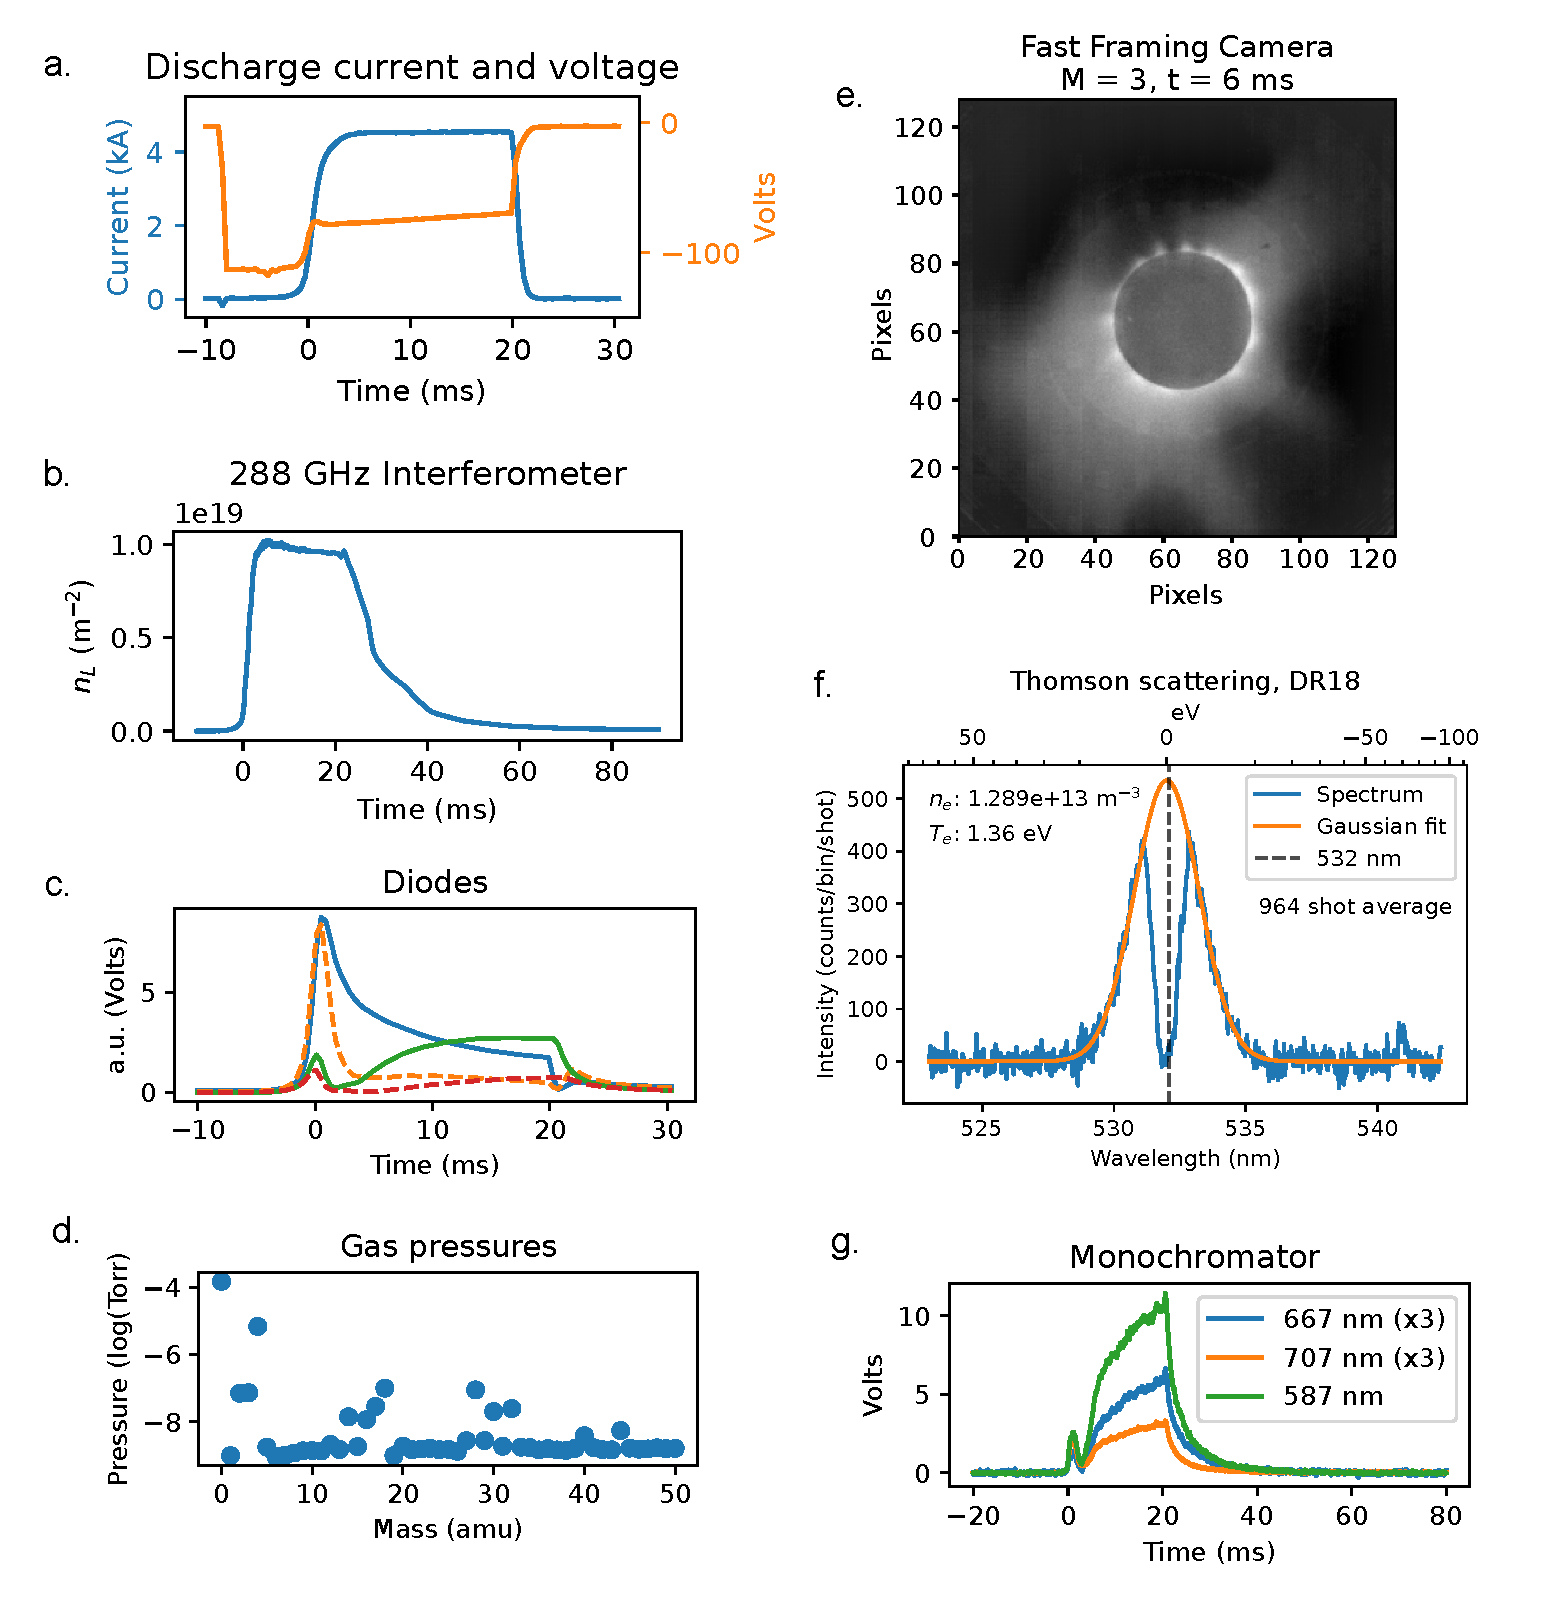
\includegraphics[width=450pt]{figures/diagnostics-examples.pdf}
	\caption[Example machine state information and diagnostic signals]{\label{fig:example-diagnostics-msi}Example diagnostic signals and machine state information from a variety of discharges.}
\end{figure}

Of the probes, only $I_\text{sat}$ was analyzed and used. The interferometer and Thomson scattering signals were also analyzed. The diode signals were unanalyzed but used in a downstream machine learning study. The spectrometer, monochromator, and diamagnetic loop remain unanalyzed and unused, but the raw signals could be useful for ML studies as will be shown with the diode signals (see chapter \ref{ch:ebm}). The fast framing camera was useful for checking probe alignment and visualizing plasma structure, but it was otherwise not used or analyzed for the downstream ML studies.

\section{Data cleaning}

$I_\text{sat}$ measurements in \texttt{DR1} that saturated either the isolation amplifier or digitizer are excluded from the dataset. Only 484 shots were removed out of $\approx$132,000, so the impact on the aggregate dataset is minimal. This signal saturation was detected while data was being taken and was corrected quickly.

Interferometer skips were occasionally seen, likely caused by large $\delta n / n$ structures combined with downsampling before conversion of the signal into a density measurement. Attempts were made to unwrap these skipping traces (see fig. \ref{fig:ifo-skip}) but without much success, so these shots were cut from the dataset.

\begin{figure}
	\centering
	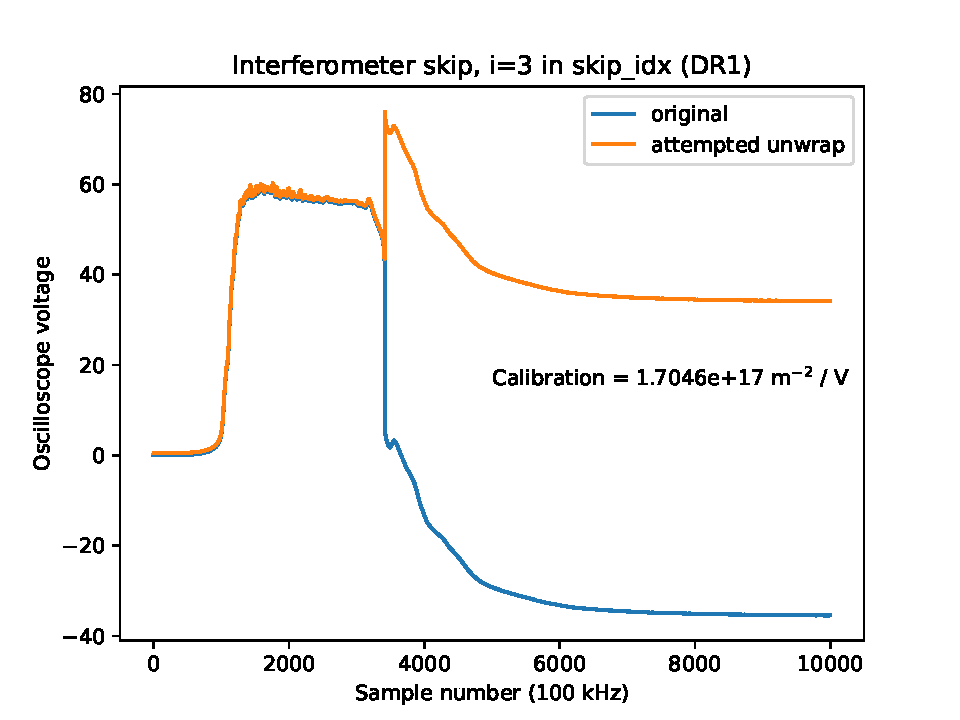
\includegraphics[width=300pt]{figures/ifo_skip_example.pdf}
	\caption[Example interferometer skips]{\label{fig:ifo-skip} An example of the interferometer skip (blue) and the attempted unwrap (orange).}
\end{figure}

The Thomson scattering (TS) diagnostic was available only for dataruns 8 and onwards in \texttt{DR1}. The TS image data did not have timestamps recorded, so a rough estimate was used based on filename and last saved time. Uncertainty in time is tolerable because conditions were identical to datarun shots for a few minutes before and after the dataruns. Fits were taken of the average over the entire datarun; each shot in a datarun has the same recorded TS temperature and density. 
Dataruns were removed if the error on the density, measured by the square root of the covariance of the fit amplitude, was greater than 50\%. Fits above that error threshold were largely unusable. A couple of dataruns looked like pure noise even when averaged over several hundred shots, but were not caught but this broad criteria. 24 dataruns remained out of 30.
In some runs there was high-pixel-frequency noise at 128 and 256 (every 4th and 2nd pixel, respectively). The fitting routine is typically insensitive to this cleaning process, but big differences can be seen in particularly low-density plasmas where the photon counts are low. An example of this process can be seen in fig. \ref{fig:TS_fit-and-FFT}.

\begin{figure}
	\centering
	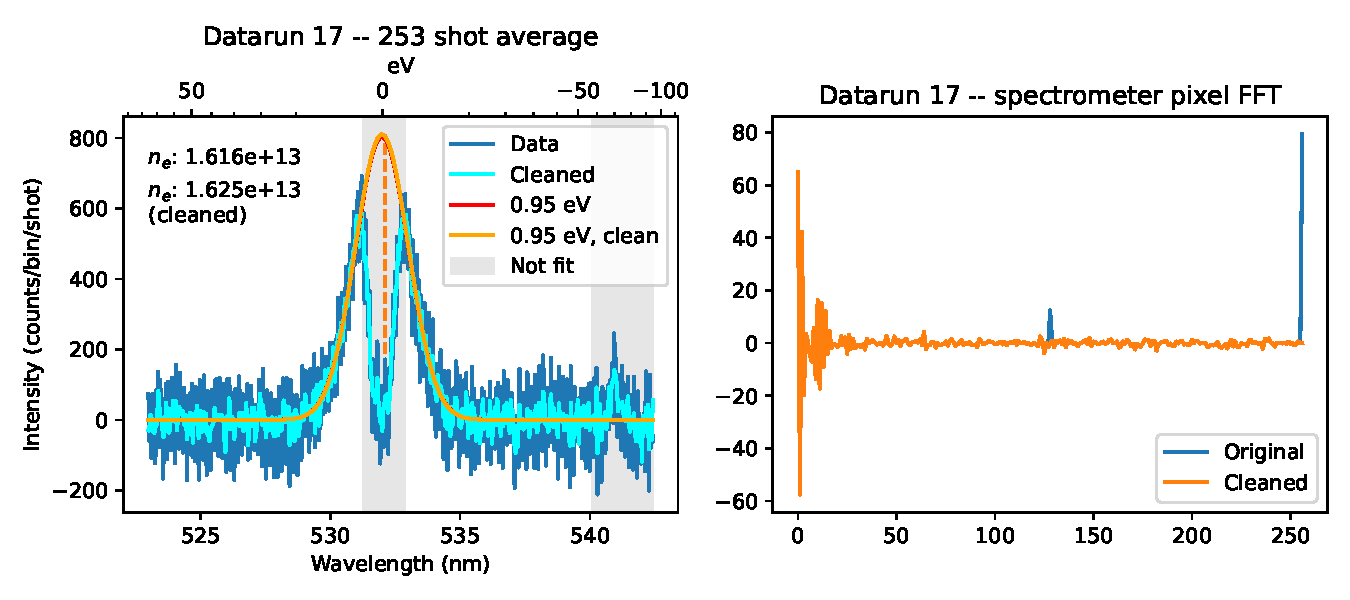
\includegraphics[width=\linewidth]{figures/TS_fit-and-FFT.pdf}
	\caption[Cleaning Thomson scattering spectra]{\label{fig:TS_fit-and-FFT} The Gaussian fit to the Thomson scattering spectrum before and after crude FFT filtering. The shaded gray region is excluded from the fitting process because they contain the region of the notch filter (the region about 532 nm) and a He-II (ion) line ($\approx 541$ nm).}
\end{figure}


\section{Data bias \label{sec:app_bias}}

Data bias and imbalance in the training set can be exacerbated by the train-test split. For the nominal test set, 8 out of the 67 dataruns were hand picked for diversity and held out from the training set. Leaving out entire dataruns -- not just shots -- is important in order to estimate model performance on new, unseen discharges in new configurations. Four dataruns from each run set were left out: from \texttt{DR1} 08, 15, 23, and 33, were held out and from \texttt{DR2}, 02, 10, 19, and 31. As will be demonstrated in chapter \ref{ch:isat-predict}, this test set appears to characterize the model performance on held out data fairly well.

The dataset predominantly contains gas puff durations of 38 ms. Only six runs in the training set have gas puff durations less than 38 ms: three have 5 ms and three have 10 ms, each having mirror ratios 1, 3, and 6 but otherwise identical configurations in an attempt to see mirror-related interchange instabilities in higher-temperature, lower-collisionality regimes. The 20 ms gas puff duration case is in the test set (\texttt{DR2} 31). This sampling bias towards the 38 ms gas puff duration suggests poor model performance is to be expected in shorter gas puff regimes. The top gas puff valve was operational for only the first nine runs of \texttt{DR2}.

\begin{figure*}
	\centering
	\includegraphics[width=\linewidth]{figures/PP1_02_isat_distribution.pdf}
	\caption[Time-averaged $I_\text{sat}$ distribution over shots]{\label{fig:PP1_02_isat_distribution}Distribution of $I_\text{sat}$ signals when averaged from 10 to 20 ms. \texttt{DR1} appears to have a more uniform distribution than \texttt{DR2} does. Combining the two datasets results in many $I_\text{sat}$ examples near 0 mA/mm$^2$ and a sharp decrease in number of examples above 10 mA/mm$^2$. From these histograms we expect or model to be biased towards fitting lower $I_\text{sat}$ values better, and to perform badly in cases with very high $I_\text{sat}$ values.}
\end{figure*}

Despite the best efforts to randomize the machine configuration, imbalance in the dataset will be present because of the relatively small amount of samples for the given actuator space. The distribution of $I_\text{sat}$ signals, averaged from 10 to 20 ms, can be seen in Fig. \ref{fig:PP1_02_isat_distribution}. The $I_\text{sat}$ distribution is clearly different for \texttt{DR1} and \texttt{DR2}, with \texttt{DR1} having a much flatter distribution. These distributions imply that if the model is constrained to sample from \texttt{DR2} via the run set flag, then the model is expected to predict a lower $I_\text{sat}$ value in general. When predicting from the model in general, performance will likely be worse for $I_\text{sat}$ values $\gtrsim 11$ mA/mm$^2$. The time-averaged $I_\text{sat}$ distribution is dissimilar between \texttt{DR1} and \texttt{DR2}: \texttt{DR1} appears to have a more uniform distribution. Combining the two datasets results in many $I_\text{sat}$ examples less than 2 mA/mm$^2$ and a sharp decrease in number of examples above 10 mA/mm$^2$. Thus, we expect the model to perform better for smaller $I_\text{sat}$ values than larger ones. 

The mix of different probe movements also leads to some imbalance in the dataset. The distribution of probe positions can be seen in fig. \ref{fig:PP1_02_x_distribution}. Notably, samples appear to drop off beyond +25 cm and -15 cm. Measurements over an x-y plane, constituting $\approx 64\%$ of all shots, are predominantly acquired overnight for maximal machine utilization. These longer dataruns lead to particular machine configurations being overrepresented in the dataset. 

\begin{figure}
	\centering
	\includegraphics[width=\linewidth]{figures/PP1_02_x_distribution.pdf}
	\caption[Distribution of probe x-coordinates in the dataset]{\label{fig:PP1_02_x_distribution}Distribution of the x-coordinate in the profiles. The increase in data points between roughly x $\approx 0$ to 30 cm is from planes instead of lines. Based on this distribution, the performance of the model is expected to be biased towards this central area.}
\end{figure}

\begin{table*}
\small
	\centering
	\caption{Data breakdown by class and dataset (percent)}
	\label{tab:data_frac}
	\begin{tabular}{lrrr|lrrr|lrrr}
		\multicolumn{4}{c|}{B source (G)} & \multicolumn{4}{c|}{B mirror (G)} & \multicolumn{4}{c}{B midplane (G)}\\
		\hline \hline
		& Train & Test & All && Train & Test & All && Train & Test & All \\
%		\cline{2-4} \cline{6-8} \cline{10-12}
		500 & 4.77 & 0 & 4.29 & 250 & 4.30 & 8.41 & 4.72 & 250 & 8.25 & 21.01 & 9.55 \\
		750 & 3.34 & 12.61 & 4.29 & 500 & 30.49 & 8.41 & 28.23 & 500 & 43.80 & 8.41 & 40.19 \\
		1000 & 43.13 & 78.99 & 46.78 & 750 & 6.68 & 16.81 & 7.72 & 750 & 6.62 & 52.19 & 11.27 \\
		1250 & 12.59 & 0 & 11.30 & 1000 & 28.85 & 57.97 & 31.82 & 1000 & 26.36 & 5.78 & 24.26 \\
		1500 & 19.23 & 0 & 17.27 & 1250 & 3.34 & 4.20 & 3.43 & 1250 & 9.24 & 0 & 8.30 \\
		1750 & 1.91 & 0 & 1.71 & 1500 & 26.34 & 4.20 & 24.08 & 1500 & 5.73 & 12.61 & 6.43 \\
		2000 & 15.03 & 8.41 & 14.35 & & & & & & & & \\
		\\
		\multicolumn{4}{c|}{Gas puff voltage (V)} & \multicolumn{4}{c|}{Discharge voltage (V)} & \multicolumn{4}{c}{Axial probe position (cm)} \\
		\hline \hline
		70 & 12.11 & 16.81 & 12.59  & 70 & 12.22 & 8.41 & 11.83    & 639 & 12.48 & 8.41 & 12.06 \\
		75 & 6.68 & 0 & 6.00     & 80 & 5.25 & 0 & 4.72      & 828 & 17.07 & 36.28 & 19.03 \\
		80 & 11.46 & 8.41 & 11.15   & 90 & 2.86 & 8.41 & 3.43      & 859 & 12.48 & 8.41 & 12.06  \\
		82 & 41.49 & 57.97 & 43.17  & 100 & 3.34 & 8.41 & 3.86     & 895 & 33.01 & 30.10 & 32.71 \\
		85 & 14.13 & 0 & 12.69   & 110 & 8.77 & 0 & 7.87     & 1017 & 12.48 & 8.41 & 12.06 \\
		90 & 14.13 & 16.81 & 14.40  & 112 & 20.62 & 0 & 18.52   & 1145 & 12.48 & 8.41 & 12.06 \\
                      & & & & 120 & 3.82 & 8.41 & 4.29     &                       & & & \\
                      & & & & 130 & 0.95 & 0 & 0.86     &                       & & & \\
                      & & & & 140 & 2.86 & 8.41 & 3.43     &                       & & & \\
                      & & & & 150 & 39.30 & 57.97 & 41.20  &                       & & & \\
		\\
		\multicolumn{4}{c|}{Gas puff duration (ms)} & \multicolumn{4}{c}{Vertical probe position (cm)}\\
		\cline{0-7} \cline{0-7}
		$38$ & 94.27 & 91.59 & 94.00 & $\approx 0$ & 36.26 & 46.08 & 37.26 & \\
		$<38$ & 5.73 & 8.41 & 6.00    & $\neq 0$ & 63.74 & 53.92 & 62.74    & \\
		\multicolumn{12}{l}{}
	\end{tabular}
\end{table*}

The distribution of the selected machine settings for all the dataruns is enumerated in Table \ref{tab:data_frac}. Despite the randomization of the settings of 44 dataruns, the distribution is often uneven. The remaining 23 non-random dataruns also contribute to the imbalance. For example, a source field of 1 kG and discharge voltage of 112 show up disproportionately in the dataset because data were collected at those settings while other equipment was being adjusted or calibrated.

\section{Azimuthal asymmetry of probe data}

Examining the data, it appears that the y coordinate is not centered properly, possibly because the telescope used to align the probes is set incorrectly. Using profiles from planar data (see the ``before'' plot in fig. \ref{fig:y-alignment_before-after}), the y-coordinate was adjusted. The probes in DR1 were adjusted upwards by +2 cm. For DR2, the y-coordinate was adjusted separately for each probe. Port 17 was adjusted 6 cm up, port 21 was adjusted 4 cm up, port 26 was adjusted 4.5 cm up, and port 33 was adjusted 3.35 cm up. This degree of error is consistent with the centering scope crosshairs having some angle error, creating a larger absolute y-axis error closer to the cathode. An example of this y-axis error and the profile after shifting the coordinates can be seen in fig. \ref{fig:y-alignment_before-after}. It is likely that this y-axis offset applies to other probes in the plasma, not just probes with $I_\text{sat}$ tips. 

\begin{figure}
	\centering
	\includegraphics[width=300pt]{figures/y-alignment_before-after.pdf}
	\caption[y-axis profile before and after shifting the y-coordinate]{\label{fig:y-alignment_before-after}An example of the y-axis profile before and after shifting the y-coordinate. The ``before'' plot (top) is obviously asymmetrical about y=0. The shift needed to center was eyeballed from the plot. Each line represents a different x position, from closest to the core (upper lines) to the edge (lower lines).}
\end{figure}

\section{Applying and improving the dataset}

The two chapters following this detail machine learning studies utilizing this dataset, though only using a subset of the diagnostics available. Much room remains for ML-based analysis of the dataset, such as including additional diagnostics, in-situ diagnostic calibration (e.g., $I_\text{sat}$ or Thomson scattering). Even though the diversity of the dataset is relatively high, many imbalances in machine inputs remain. More data with additional (pseudo-)random samples from broader parameter ranges would be very beneficial in improving downstream ML tasks. Pushing the boundaries of the machine parameters could also lead to discovery and exploitation of new operational modes of the LAPD which could prove beneficial.


\graphicspath{{Chapters/Chapter_isat-predict/}}

\chapter{Optimizing mirror configurations in the LAPD using machine learning}
\label{ch:opt_ML}

%\documentclass[aip,
%	pop,
%	reprint,
%	floatfix]{revtex4-2}
%
%%\bibliographystyle{iopart-num}
%\bibliographystyle{aipnum4-2}
%%\usepackage{citesort}
%
%\usepackage{graphicx}
%\usepackage[left=1in, right=1in,  top=1in, bottom=1in]{geometry}
%\usepackage{amsmath}
%\usepackage{amssymb}
%%\usepackage[strings]{underscore}
%\usepackage{subfig}
%\usepackage{float}
%\input{markers.tex}
%
%\usepackage[utf8]{inputenc}
%\usepackage[T1]{fontenc}
%\usepackage{bm}% bold math
%
%\begin{document}
%\preprint{AIP/123-QED}
%
%\title[]{Machine-learned trends in mirror configurations in the Large Plasma Device}
%
%\author{Phil Travis$^1$, Jacob Bortnik$^2$, Troy Carter$^{1,3}$}
%
%\address{Department of Physics and Astronomy, University of California, Los Angeles, CA, USA}
%\address{Department of Atmospheric and Oceanic Sciences, University of California, Los Angeles, CA, USA}
%\address{Oak Ridge National Laboratory, Oak Ridge, TN, USA}

%\author{}
%\email[]{Your e-mail address}
%\homepage[]{Your web page}
%\thanks{}
%\altaffiliation{}
%\affiliation{}

%\ead{phil@physics.ucla.edu}
%\vspace{10pt}
%\begin{indented}
%\item[]Fall/Winter 2024
%\end{indented}

\begin{abstract}
%Neural network (NN)-based machine learning (ML) techniques enable extraction of trends directly from experimental data, which is the first step towards automating plasma science.

This study demonstrates the efficacy of machine learning (ML)-based trend inference using data from the Large Plasma Device (LAPD).
%The LAPD is a flexible basic plasma science device with a high discharge repetition rate (0.25-1 Hz) and reproducible plasmas capable of collecting high-spatial-resolution probe measurements. A diverse dataset is collected through random sampling of LAPD operational parameters, including the magnetic field strength and profile, fueling settings, and the discharge voltage. 
Neural network (NN) ensembles with uncertainty quantification are trained to predict time-averaged ion saturation current ($I_\text{sat}$ — proportional to density and the square root of electron temperature) at any position within the dataset domain. Model-inferred trends, such as the effects of introducing mirrors or changing the discharge voltage, are consistent with current understanding. In addition, axial variation is optimized via comprehensive search over $I_\text{sat}$ predictions. Experimental validation of these optimized machine parameters demonstrate qualitative agreement, with quantitative differences attributable to Langmuir probe variation and cathode conditions. This investigation demonstrates, using ML techniques, a new way of extracting insight from experiments and novel optimization of plasmas. The code and data used in this study are made freely available.

This chapter is based on the publication (currently under review) in the Physics of Plasmas titled ``Machine-learned trends in mirror configurations in the Large Plasma Device'' by myself, Prof. Jacob Bortnik, and Prof. Troy Carter. The goals of this work are to show what a solid, validated machine learning study looks like, and how ML can be useful in understanding operating plasma devices.

\end{abstract}

%\pacs{}% insert suggested PACS numbers in braces on next line

%\maketitle %\maketitle must follow title, authors, abstract and \pacs

\section{Introduction}

Understanding and controlling plasma behavior in fusion devices is necessary for developing efficient fusion reactors for energy production. Because of the complex, high-dimensional parameter space, traditional experimental approaches are often time-consuming and require careful planning. This work explores how machine learning (ML) techniques can accelerate this understanding by studying the effect of machine parameters in a basic magnetized plasma device. Trend inference is this process of relationship discovery. While ML methods, particularly neural networks (NNs), have become increasingly prevalent in fusion research for control and stabilization, their application to systematic trend discovery remains largely unexplored.

Many studies have used ML for profile prediction on a variety of tokamaks, particularly for real-time prediction and control. For example, NNs were used to predict electron density, temperature, and other quantities in DIII-D \cite{abbate_data-driven_2021}, and reservoir NNs have demonstrated the ability to quickly adapt to new scenarios or devices \cite{jalalvand_real-time_2022}. Temporal evolution of parameters has been successfully modeled using recurrent neural networks (RNNs)\cite{char_full_2024} for multiple devices, including the EAST\cite{wan_east_2022} and KSTAR tokamaks\cite{seo_feedforward_2021,seo_development_2022}. These predictions enabled training of a reinforcement learning-based controller\cite{seo_feedforward_2021,seo_development_2022}. In addition, a decision tree-based controller was trained to maximize $\beta_N$ while avoiding tearing instabilities\cite{fu_machine_2020} on DIII-D. Electron temperature profiles have also been predicted using dense NNs on the J-TEXT tokamak \cite{dong_machine_2021}.

A parallel focus has been on instability prediction and mitigation in tokamaks, particularly of disruptions. Notable achievements in disruption prediction include RNN-based disruption prediction \cite{kates-harbeck_predicting_2019} and random forest approaches\cite{rea_real-time_2019}, with a comprehensive review available by Vega et al \cite{vega_disruption_2022}. Recent work has extended to active control, such as the mitigation of tearing instabilities in DIII-D using reinforcement learning \cite{seo_avoiding_2024}. 

While ML has proven effective for prediction and control tasks, inferring trends using data-driven methods has been relatively uncommon. Notable exceptions include finding scaling laws on the JET tokamak\cite{murari_investigating_2020} via classical ML techniques and the development of the Maris density limit\cite{maris_correlation_2024} which outperforms other common scalings (including the Greenwald density limit) in predictive capability.

The use of machine learning and Bayesian inference in fusion research has been recently reviewed by Pavone et al.\cite{pavone_machine_2023}

Outside of magnetized plasmas, the laser plasma community has embraced ML techniques for various applications, enumerated in a review by Dopp et al.\cite{dopp_data-driven_2023}. 
Data-driven plasma science in general has been reviewed by Anirudh et al.\cite{anirudh_2022_2023}
Notably, a similar quasi-random method (Sobol sequences) was used to collect a spectroscopy dataset on a plasma processing device over diverse machine settings \cite{daly_data-driven_2023}. This process is similar to what is performed in our work here, but a generative variational autoencoder was instead trained to be used as an empirical surrogate model.

This work advances data-driven methods in plasma physics by taking these methods one step further: instead of learning a model for particular task (e.g., disruption prediction or profile prediction), we infer learned trends directly from the model itself. 
%Trend inference applied in this way is new to magnetized plasma research. 

The goal of this study is to develop a data-driven model that can provide insight into the effect of machine parameters on plasmas produced in Large Plasma Device (LAPD) in lieu of a theoretical model. In contrast with tokamaks and other fusion devices, the LAPD is particularly well-suited for ML data collection because of its flexibility and high repetition rate. We demonstrate the capability to infer trends in a particular diagnostic signal, the time-averaged ion saturation current ($I_\text{sat}$), for any mirror (or anti-mirror) field geometry in a variety of machine configurations. Langmuir probes are commonly used to measure density, temperature, and potential in virtually all plasma devices in low-temperature (less than 10s of an eV) regimes. The $I_\text{sat}$ signal in particular is almost always used in the LAPD for calculating local plasma density.

This study performs two firsts in magnetized plasma research: using NNs to directly infer trends and collecting data efficiently with partially-randomized machine parameters. We also demonstrate optimizing LAPD plasmas given any cost function by minimizing axial variation in $I_\text{sat}$. This global optimization is only possible using ML techniques. This work demonstrates the usefulness of a pure ML approach to modeling device operation and shows how this model can be exploited. We encourage existing ML projects and experiments to consider this approach if possible. Acquiring sufficiently diverse datasets may require assuming some risk because diverse data, such as discharges from randomly sampled machine settings, may not be amenable to conventional analysis techniques.

%\todo{Reconsider this paragraph}
%
All the processed data used for training the models in this study are freely available\cite{phil_travis_2025_15007853} (see section \ref{app:repo}). Other devices have also made data publicly available. Namely, data for H-mode confinement scaling has been available since 2008\cite{roach_2008_2008}, and more recently some MAST\cite{jackson_fair-mast_2024} and all LHD\cite{lhd_data} data are now publicly available.  

%This paper is organized as follows: Section \ref{sec:data} discusses the LAPD and the data acquisition methodology. Sections \ref{sec:model_dev} and \ref{sec:uncertainty} detail development of the model and uncertainty quantification. Section \ref{sec:validation} presents model validation, followed by trends in discharge voltage and gas puff duration in Section \ref{sec:trends}. Section \ref{sec:optimization} demonstrates optimization of the axial $I_\text{sat}$ profile, with the discussion and conclusion in sections \ref{sec:isat-predict_discussion} and \ref{sec:isat-predict_conclusion}.

\begin{figure*}
	\centering
	\includegraphics[width=\textwidth]{figures/LAPD+coordinates.pdf}
	\caption[Cartoon of the experiment setup]{\label{fig:LAPD_coords}A cartoon of the Large Plasma Device, the coordinate system used, examples of a mirror and anti-mirror magnetic field configuration, and probe locations used in this study. The source, mirror, and midplane regions are labeled; the three fields were programmed independently.}
\end{figure*}

\section{Processing of $I_\text{sat}$ signals}

The ion saturation current, denoted as $I_\text{sat}$, is obtained by applying a sufficiently negatively bias to a Langmuir probe to ensure the exclusive collection of ions. This collected current is proportional to $S n_e \sqrt{T_e}$, where $n_e$ and $T_e$ are the electron density and temperature, and $S$ is the effective probe collection area. To account for differences in probe tip geometry, the $I_\text{sat}$ values are normalized to area. Under typical conditions, an $I_\text{sat}$ value of 1 mA/mm$^2$ corresponds to $n_e \approx 1\text{-}2\times 10^{12}$ cm$^{-3}$ for a $T_e$ from 4 to 1 eV.

$I_\text{sat}$ measurements were averaged over 10 to 20 ms to exclude plasma ramp-up and fluctuations. Example $I_\text{sat}$ probe data can be seen in fig. \ref{fig:PP1_time-series-example} along side gas puff timings.  For the probe tip that was on the same shaft as the swept probe (in \texttt{DR2}), the signal was instead averaged over when the bias voltage on the swept tip was held constant at the lowest value. A 40 $\mu$s (250 sample) buffer was used after the sweep was turned off to minimize the impact of transient conditions. A comparison of the full trace and the trace with the swept portion excluded can be seen in fig. \ref{fig:PP1_swept_probe}. Notably, the measured $I_\text{sat}$ value does not attain a steady state before the discharge shuts off. 

\begin{figure}
	\centering
	\includegraphics[width=270pt]{figures/PP1_isat_swept_probe.pdf}
	\caption[$I_\text{sat}$ traces from the swept probe]{\label{fig:PP1_swept_probe}$I_\text{sat}$ traces from the swept probe (port 26) from \texttt{DR2} datarun 03, shot 1 of 6. The orange curve is excluding times when a sweep is active on an opposing tip. }
\end{figure}

Profile evolution is not studied to minimize computational requirements. $I_\text{sat}$ characteristics vary significantly between axial (z) position machine parameters. For $I_\text{sat}$ measurements on the same probe as a Langmuir sweep (\texttt{DR2} port 26, z=863 cm), the averaging process excludes the sweep period with an additional 40 $\mu$s buffer. $I_\text{sat}$ measurements in \texttt{DR1} that saturated either the isolation amplifier or digitizer are excluded from the dataset. Only 484 shots were removed out of $\approx$132,000, so the impact on the aggregate dataset is minimal. 

\begin{figure}
	\centering
	\includegraphics[width=370pt]{figures/PP1_time-series-example.pdf}
	\caption{\label{fig:PP1_time-series-example}Gas puff timings and example $I_\text{sat}$ time series at three different z-axis locations from three different dataruns. Note that some discharges do not achieve steady state in $I_\text{sat}$. }
\end{figure}

While $I_\text{sat}$ exhibits a small degree of shot-to-shot variation, the present model only learns the expected value, leaving distributional modeling to future generative approaches. An example of these $I_\text{sat}$ profiles and the six-shot variance can be seen in fig. \ref{fig:PP1_isat_example}.

\begin{figure}
	\centering
	\includegraphics[width=270pt]{figures/PP1_isat_example_bars.pdf}
	\caption[Examples of $I_\text{sat}$ profiles from \texttt{DR2}]{\label{fig:PP1_isat_example}Examples of $I_\text{sat}$ profiles from \texttt{DR2} run 15. The bars represent the minimum and maximum of the six $I_\text{sat}$ measurements taken at that position. }
\end{figure}

\section{Model development and training}
\label{sec:model_dev}

\subsection{Model inputs}

Neural network inputs comprise 12 variables: source field, mirror field, midplane field, gas puff voltage, discharge voltage, gas puff duration, probe coordinates (x, y, z), probe rotation, run set identifier, and top gas puff flag. These variables can be interpreted as six control parameters, four probe coordinates, and two flags. These inputs are mean-centered and normalized to the peak-to-peak value with no outliers in the dataset. The baseline models trained in section \ref{sec:baselines} did not contain the run set identifier or top gas puff flag.

\subsection{Training details}

For initial experiments in training the model, a mean-squared error (MSE) loss is used:
\begin{equation}
	\mathcal{L}_\text{MSE}=\frac{1}{m}\sum_{i=1}^m \left(f\left(x_i\right) - y_i \right)^2
\end{equation} 
where $x_i$ represents the input vector for the $i$th example, $y_i$ the target measurement, $m$ the batch size, and $f$ the NN. During training, overfitting was assessed via the validation set MSE with a traditional 80-20 train-validation random split. Unless stated otherwise, a dense neural network, 4 hidden layers deep and 256 units wide (201,218 parameters for $\beta$-NLL loss, 200,962 parameters for MSE loss), was trained with AdamW using a learning rate of $3\times10^{-4}$. Leaky ReLU activations (the nonlinearities in the NN) and adaptive gradient clipping\cite{seetharaman_autoclip_2020} (cutting gradients norms above the 90th percentile of recent norms) were used to mitigate vanishing gradients and mitigate exploding gradients, respectively. The models were evaluated after training concluded at 500 epochs.

\subsection{Validating the training pipeline}

ML training processes are relatively simple but bugs, particularly in the data pipeline, can be insidious and can affect final model performance even though training looks fine. Here we validate the data pipeline (which should be performed in every ML study) to verify that the model is training and expected and that there is no accidental data leakage between the train and test sets. Andrej Karpathy's advice for training neural networks \cite{karpathy_recipe_2019} was used as a template for verifying the training procedure used in this project. The data fed into the model immediately before the forward pass (and subsequent backpropagation) was stored and verified: the data are correctly randomly shuffled in each batch. Each epoch contains the same random shot order. To validate the data pipeline, a simple dense model (4 layers, 512 wide with one output; 794113 parameters, tanh activations) was trained. The model is also overfit on a single batch (128 examples) of training data to make sure that training progresses as expected. A deep double descent is observed as expected \cite{nakkiran_deep_2019,schaeffer_double_2023}. Training on a batch of 8 examples reaches $\approx$ 0 training loss after 50 steps. Plots of the train and validation losses can be seen in Fig. \ref{fig:PP1_overfit_losses}.

Multiple models were trained with varying depths and widths to verify that training loss decreases with increased model capacity. Doubling the layer width from 512 to 1024 moderately decreases the training loss; doubling the depth of the network from 4 to 8 layers has a larger impact. Increasing the width further to 2048 and depth to 12 layers has a dramatic impact on training loss, so this model and dataset are behaving nominally. The model pipeline is training and performing as expected, so we proceed.

\begin{figure}
	\centering
	\includegraphics[width=300pt]{figures/PP1_overfit_losses.pdf}
	\caption[Training and validation losses when overfitting the model]{\label{fig:PP1_overfit_losses}Training and validation losses when overfitting the model. A deep double descent in the validation losses is observed when fitting a single batch of 128 examples. The 8-example batch hits near-zero loss after 50 steps. This process verifies our training process is functioning as expected. The spikes are from exploding gradients which can be mitigated by clipping the gradients. A model trained on blank data is also shown as the black dotted line.}
\end{figure}

\subsection{Baselines for mean-squared error}
\label{sec:baselines}

A model was first trained with zeroed-out inputs as a baseline and to validate the data pipeline. This model effectively has only a single, learnable bias parameter at the input. This process yields a validation loss (simply MSE in this case) of 0.036. 

%A linear model, though incapable of reasonably fitting the data, was trained as a performance baseline and to validate the data pipeline. This baseline linear model reaches a training and validation loss (MSE) of around 0.014. These initial models used \texttt{tanh} activations, though the impact of using a different activation function is minimal in these cases.
%\subsubsection{Baseline linear-like models (\texttt{DR2})}
A linear model obviously cannot fit the dataset (see the nonlinear shape of the profiles in fig. \ref{fig:PP1_isat_example}). However, a simple (and mostly linear) model can provide a performance baseline to help spot bugs when training more complex models. Since the x- and y- profiles have a approximate $\tanh$ shape, a feature is added at the linear model input stage for the x and y coordinates: $x_\texttt{tanh} = c \cdot \tanh\left(\left|x + s\right| \cdot a + b \right)$ where $s, a, b, c$ are trainable parameters (independent for each coordinate; $c$ is superfluous). This function was chosen to give the linear model the capability of expressing $\tanh$-like curves. The performance of the linear model on \texttt{DR2} data, with and without the $\tanh$ features, can be seen in fig. \ref{fig:PP1_linear_simple_data}. This baseline linear-like model reaches a training and validation loss of around 0.011, with the RMSE $=\sqrt{\text{loss}} \sim 0.1$. The linear-only model is marginally worse with losses at around 0.014.

\begin{figure}
	\centering
	\includegraphics[width=300pt]{figures/PP1_linear_simple_vs_data.pdf}
	\caption[Linear predictions of $I_\text{sat}$ profiles]{\label{fig:PP1_linear_simple_data}$I_\text{sat}$ profiles and predictions for ports 17 and 33 based on inputs from \texttt{DR2} run 08 using a liner and linear-with-tanh models. \texttt{DR2} run 08 is in the training set. The ``data'' points are averaged over six shots. Run 08 was chosen for its representative performance; ports 17 and 33 were chosen to demonstrate the maximal axial variation (across 511 cm). These models fail to describe the data accurately.}
\end{figure}

This feature engineering-like approach can continue. For example, the width of the profile is largely controlled by magnetic field configuration of the device, particularly by $\sqrt{B_\text{midplane}/B_\text{source}}$. This behavior can be added to this model, either as a new feature or as a custom relationship in the model. Note that, as seen in fig. \ref{fig:PP1_linear_simple_data}, the width of the profile also depends on the axial coordinate. Combined with other coordinates and actuators, like discharge voltage and gas pressure, the number of possible features or function space grows combinatorially, making this custom fitting process difficult and tedious to design and test by hand. The obvious solution would be to use symbolic regression or fitting to a function library which may be  ideal methods if simple profile prediction were the final goal. However, we are ultimately interested inferring trends in a much more complex input space where neural networks are more flexible and accurate. If NNs do face generalization issues, symbolic regression or a SINDy-like approach can used instead, albeit with limited applications. Symbolic methods are appealing because the fits are simple. However, even though a simple equation may fit the data well, it does not necessarily provide insight or relate to the underlying physics; using a freeform fitting function like a neural network is more appropriate in this use case.

A summary of these baselines is seen at the top of Table \ref{tab:loss_summary}.


\begin{table}
	\small
	\centering
	\caption{Summary of test set losses for different training data and ensembles}
	\label{tab:loss_summary}
	\begin{tabular}{l l l}
		Model & MSE $\times 10^{-3}$ \\
		\hline
		Zeroed-input & 36  (validation) \\
		Linear model & 14 (validation) \\
		Linear with tanh features & 11 (validation)\\
		\hline
		9 dataruns & 7.0\\
		19 dataruns & 6.9 \\
		29 dataruns & 4.2 \\
		39 dataruns & 4.1 \\ 
		49 dataruns & 3.4 \\
		\texttt{DR1} only & $6.4$ \\
		\texttt{DR2} only & $5.4$ \\
		Full set, large model & $2.8$ \\
		Full set average & $3.6 \pm 0.56$ \\
		Full set ensemble & $2.9 \pm 1.1$ \\
		\hline
		``Run set'' flag average & $2.1 \pm 0.15$ \\
		``Run set'' flag ensemble & $1.9 \pm 0.64$ \\
		``Top gas puff'' flag & 1.8 \\
		
	\end{tabular}
\end{table}

\subsection{Effects of training set and model sizes}
 
To study the effects of reduced diversity, the number of unique dataruns in the training set was systematically reduced while evaluating on a fixed test set. The test set loss monotonically increased with this decrease in datarun count. Part of this decrease may be caused by a simple reduction in training set size. In addition, models were individually trained and evaluated on \texttt{DR1} only or  \texttt{DR2} only. When evaluated on the left-out run set, the test set losses were high, near or above the zero-input baseline of $3.6 \times 10^{-2}$. This result suggests that both run sets contain significant information missing in the other, and training on both provides beneficial information on the structure of the $I_\text{sat}$ measurement despite different probe calibrations and cathode state.

A larger model, consisting of a 12-deep 2048-wide dense network, was trained on the full training dataset, evaluated at 30 epochs. This larger model yielded a test MSE of $2.8 \times 10^{-3}$, indicating that these NNs are behaving as expected. Longer training or larger models may yield better test set results, but will likely not come close to the training and validation losses which are on the order of $10^{-5}$. Combined models with differing initializations (an ensemble), were trained to measure the MSE variance over model parameters which was about 16\%. When the $I_\text{sat}$ predictions were averaged, the test set MSE was $2.9 \pm 1.1 \times 10^{-3}$, achieving the best performance for that model size. These test set losses are also seen in Table \ref{tab:loss_summary}. 

%One unexpected result is that models trained on a single run set appear to perform worse when evaluated on the test set (from that particular run set) compared to the mixed training set of the same size (green arrows vs blue x). This fact indicates that mixing dataruns, despite different probe calibrations and cathode state, provides beneficial information on the structure of the $I_\text{sat}$ measurement. This model is able to leverage information in both dataruns despite potential differences in the effect of the machine settings and the cathode condition.

%Skepticism is warranted, however, because the variance over model parameters may be able to account for most, if not all, of the performance difference as suggested by the full-set ensemble. The variance caused by random datarun selection may also account for some of the difference; this variance was not measured and could be considerable. The effect of varying the training and test datasets will be discussed in section \ref{subsec:cross-validation}.

\subsection{Improving performance with machine state flags}

Data from \texttt{DR1} and \texttt{DR2} were collected 14 months apart leading to differing machine states. In \texttt{DR1}, only one turbo pump was operating leading to much higher neutral pressures than in the \texttt{DR2} run set. A new parameter (mean-centered and scaled) was added to the inputs to distinguish between these two run sets. All the predictions in this study use the \texttt{DR2} run set flag (a value of 1.0) because turning off the turbopumps is not a commonly desired mode of operating the LAPD. The inclusion of this parameter also provides the model the ability to distinguish between the probe calibration differences between \texttt{DR1} and \texttt{DR2}. An ensemble prediction with this run set flag brings the test set MSE down to $1.9 \times 10^{-3}$.  

A flag indicating when the top gas puff valve was enabled in \texttt{DR2} was also added to all training data, allowing the model to further distinguish between different fueling cases. The addition of this flag incrementally improved test set MSE to $1.8 \times 10^{-3}$. The effect on MSE on the inclusion of these new parameters is compared to the performance of other models in Table \ref{tab:loss_summary}. 

\subsection{Learning rate scheduling}
Modifying the learning rate over time (scheduling) is known to improve model learning. The following schedules were compared: constant learning rate ($\gamma = 3 \times 10^{-4}$), $\gamma \propto \text{epoch}^{-1}$, $\gamma \propto \exp{(-\text{epoch})}$, and $\gamma \propto \text{epoch}^{-1/2}$. The epoch is the training step divided by the number of batches in one epoch, so ``epoch'' in this case takes on a floating-point value. $\gamma \propto \text{epoch}^{-1}$ appears to give the best test set loss by a test MSE difference of $1 \times 10^{-4}$, and any schedule beats a constant learning rate by a difference of $2-4 \times 10^{-4}$. 
%The differences in test set losses are small, but the difference in training and validation losses are quite significant, with the constant learning rate loss being three times higher. 

%\begin{enumerate}
%	\item Baseline models plot (done)
%	\item Losses vs dataset diversity (done)
%\end{enumerate}
 
%\begin{figure}
%	\centering
%	\includegraphics[width=\columnwidth]{figures/PP1_test-loss_vs_dataset.pdf}
%	\caption[Effect of dataset diversity on MSE]{\label{fig:PP1_validation_diversity}Several models were trained with dataruns cut out, decreasing the diversity of the training set. The test set was kept fixed. Loss on the test set monotonically increases with decreasing diversity. }
%\end{figure} 

\section{Uncertainty quantification}
\label{sec:uncertainty}

\subsection{$\beta$-NLL loss}

Instead of predicting a single point, the model can predict a mean $\mu$ and variance $\sigma^2$ using the negative-log likelihood (NLL) loss \cite{nix_estimating_1994,lakshminarayanan_simple_2017} by assuming a Gaussian likelihood. An adaptive scaling factor $\text{StopGrad}(\sigma_i^{2\beta})$ is introduced that can be interpreted as an interpolation between an MSE loss and Gaussian NLL loss, yielding the $\beta$-NLL loss:

\begin{equation}
%	\begin{multline}	
	\mathcal{L}_{\beta-\text{NLL}} = \frac{1}{2}\left( \log{\sigma^2_i(\mathbf{x}_n)} +\frac{\left(\mu_i(\mathbf{x}_n) - y_n\right)^2}{\sigma^2_i (\mathbf{x}_n)} \right) \text{StopGrad}\left(\sigma_i^{2\beta}\right)
	\label{eq:loss_beta-NLL}
%	\end{multline}
\end{equation}

for example $n$ and model $i$, with an implicit expectation over training examples. $\beta=0$ yields the original Gaussian NLL loss function and $\beta=1$ yields the MSE loss function. This factor improves MSE performance by scaling via an effective learning rate for each example (which necessitates the \texttt{StopGrad} operation) \cite{seitzer_pitfalls_2022}, and improves both aleatoric and epistemic uncertainty quantification \cite{valdenegro-toro_deeper_2022}. $\beta=0.5$ was used by default in this study. This $\beta$-NLL loss function also improved training stability.

This NLL-like loss assumes the prediction -- the likelihood of $y$ given input $\mathbf{x}$: $p(y|\mathbf{x})$ -- follows a Gaussian distribution. Treating each prediction as an independent random variable (considering each model in the ensemble is sampled from some weight distribution $\theta \sim p(\theta | \mathbf{x}, y)$) and finding the mean of the random variables yields a normal distribution with mean $\mu_* (\mathbf{x}) = \langle \mu_i(\mathbf{x}) \rangle $ and variance $\sigma^2_* = \langle \sigma^2_i(\mathbf{x}) + \mu^2_i(\mathbf{x}) \rangle - \mu^2_* (\mathbf{x})$ where $\langle \rangle$ indicates an average over the ensemble.

The loss function for one of the NNs in an ensemble is seen in fig. \ref{fig:beta-NLL_loss-mse}. The MSE decreases monotonically for the training and validation set, but does not for the test set. The loss function can no longer be interpreted as a log-likelihood because of the effective per-example learning rate set by the $\beta$ term in the loss (eq. \ref{eq:loss_beta-NLL}). Note that early stopping (at around 8 epochs) would improve the test set loss, but the MSE would still be several factors higher than after 500 epochs. Early stopping was not explored in this study.

\begin{figure}
	\centering
	\includegraphics[width=300pt]{figures/beta-NLL_loss-mse.pdf}
	\caption[The loss and MSE for the training, validation, and test sets]{\label{fig:beta-NLL_loss-mse}The loss and MSE for the training, validation, and test sets over the entire training duration of 500 epochs. The inclusion of the $\beta$ term in the loss function -- interpreted as a per-example learning rate -- makes the loss function no longer interpretable in simple terms. The mean-squared error benefits from longer training for all sets.}
\end{figure}

The ensemble predictive uncertainty can be broken down into the aleatoric and epistemic components \cite{valdenegro-toro_deeper_2022}: the aleatoric uncertainty is $\langle \sigma^2_i (\mathbf{x}) \rangle$ and the epistemic uncertainty is $\langle \mu^2_i (\mathbf{x}) \rangle - \mu^2_* (\mathbf{x}) = \text{Var}\lbrack\mu_i (\mathbf{x}) \rbrack$. The intuition behind these uncertainties is that the random fluctuations in the recorded data are captured in the variance of a single network, $\sigma^2_i$. If the choice of model parameters were significant, we would expect the predicted mean for a single model, $\mu_i$, to fluctuate as captured by $\text{Var}\lbrack\mu_i (\mathbf{x}) \rbrack$. 

%Using the $\beta$-NLL loss, the model is slightly better calibrated, but barely worth discussing. 

%\begin{enumerate}
%	\item Cross validation plot (done)
%	\item z-score histogram (done)
%	\item Calibration via weight decay scan (done)
%	\item Profiles with different weight decays (done)
%\end{enumerate}

\subsection{Cross-validation MSE}

For cross-validation, multiple train-test set pairs were created. Test set 0 comprises deliberately chosen dataruns to encompass a diverse set of machine settings and probe movements. The other six datasets were  compiled with randomly chosen dataruns (without replacement) while keeping the number of dataruns from \texttt{DR1} and \texttt{DR2} equal. Seven model ensembles (5 NNs per ensemble -- 35 NNs total) were trained to evaluate the effect of test set choice on model MSE. The test set MSE performance can be seen in fig. \ref{fig:cv-beta-NLL-test-mse}, and the training MSE performance in fig. \ref{fig:cv-beta-NLL-train-mse}. The median ensemble test set MSE for these seven sets was $2.13 \times 10^{-3}$ with a mean of $3.6 \times 10^{-3}$. The handpicked dataset had an ensemble test set MSE of $1.85 \times 10^{-3}$, indicating that the choice of dataruns was adequately representative. This median MSE will be used to estimate model prediction error in addition to uncertainty quantification. This cross-validation also provides an error estimate if the models were to be trained on \emph{all} dataruns. Ensembles always out-performed the average error of single-model predictions.

All validation set MSEs fall between $1$ and $6 \times 10^{-5}$, with the average training MSE falling within that range as well. These MSEs indicate that the model is able to fit the training data to a high degree of accuracy regardless of which dataruns are held out. The loss and MSE curves over training epochs can be seen in the appendix in fig. \ref{fig:beta-NLL_loss-mse}.

%The median of the cross-validation ensemble performance for the test set is roughly the same as the MSE for testing set 0, so our choice of dataruns for the testing set appears reasonable. The calibration of the model also varies across dataruns, which can be investigated. Ideally, knowing the models train well and having an idea of the cross-validated error, it should be possible to train on all data in it's entirety and still have some reasonable estimate of the error of the model.

\begin{figure}
	\centering
	\includegraphics[width=260pt]{figures/cv-beta-NLL-valid-mse.pdf}
	\caption[Cross-validation test set error]{\label{fig:cv-beta-NLL-test-mse}Model performance as measured by MSE over test sets with different dataruns. Test set 0 is the hand-picked dataset, and the rest were randomly compiled without replacement (though separate for \texttt{DR1} and \texttt{DR2}). The number at the bottom of the bar chart is the number of shots in the testing set. The median test set performance is very close to the hand picked (set 0) performance. Ensembles always out-perform the average single-model prediction.}
\end{figure}

\begin{figure}
	\centering
	\includegraphics[width=260pt]{figures/cv-beta-NLL-train-mse.pdf}
	\caption[Cross-validation training set error]{\label{fig:cv-beta-NLL-train-mse}See caption for fig. \ref{fig:cv-beta-NLL-test-mse}. Note that the training loss is dramatically less than the testing loss, but otherwise there is no discernible trend.}
\end{figure}

\subsection{Model calibration via weight decay}

The predicted uncertainty may not provide an accurate range of $I_\text{sat}$ values when compared to the measured value. Calibrating the model means changing the predicted uncertainty range so that the measured values fall within that range according to some distribution, such as a Gaussian in this case. One of the ways assessing this calibration is by the z-score of predictions, where $z_n= \left(x_n - \mu_n \right) / \sigma_n(x_n)$ for example $x_n$, predicted mean $\mu_n$, and standard deviation $\sigma_n$. Perfect model calibration would lead to identical z-score distribution $\mathcal{N}(\mu=0, \sigma=1)$ for the training a test sets. When evaluated on the training set, the distribution should be a Gaussian with a standard deviation of 1. The z-score disbitrubtions for the train and test sets with a model weight decay of 0 can be seen in fig. \ref{fig:z-score_wd-0_paperplot}.

\begin{figure}
	\centering
	\includegraphics[width=300pt]{figures/z-score_wd-0_paperplot.pdf}
	\caption[Z-score distributions for the training and test sets for $\lambda = 0$]{\label{fig:z-score_wd-0_paperplot}Z-scores for the training and testing set for the model with a weight decay coefficient $\lambda$ of zero. The magnitude of counts for the test set is scaled up by a factor of 8.8 (the train-to-test example ratio). The histograms are clipped between z of -8 and 8 with a bin width of 0.25; the spike at the negative side of the test set histogram is from the long tail.}
\end{figure}

Increased weight decay can lead to better model calibration \cite{guo_calibration_2017}. Weight decay penalizes large parameter values by adding the L2 norm of model weights to the loss. Model ensembles were trained with weight decay coefficients between 0 and 50 to determine the best calibrated model determined by the distribution of z-scores of the training and test sets. The results of this weight decay scan are seen in Fig. \ref{fig:beta-NLL_wd_model_performance}. Increasing the weight decay increases the test MSE and decreases its z-score standard deviation. This large standard deviation is caused by outliers. Excluding z-scores magnitudes above 10, or 4.4\% of the test set, yields a standard deviation of 2.53. This long tail indicates that the distribution of predictions on the test set is not Gaussian. Nonetheless, the trend remains that increasing weight decay leads to smaller test set z-score standard deviations. However, the test set MSE increases after a weight decay of 1. This increase in test MSE implies that the model is making less accurate predictions but is better calibrated. Highly biased models are better calibrated, but come at great expense of mean prediction error. At the weight decay value of 50, the model has worse error than a linear model. Despite the attempts using weight decay, the model never becomes well-calibrated: the predicted uncertainty is always too low by a factor of 2 to 5. 

%As seen in Fig. \ref{fig:extrapolation-variance_wd-comparison}, the uncertainty predictions are not useful except for models with low weight decays.
 
%A comparison of many different weight decay coefficients can be seen in Fig. \ref{fig:weight_decay-model}; 20 was determined to be a good weight decay value. The ``knee'' value of 30 was not chosen because the distribution of z-scores looked odd. The training and test z-score distribution can be seen in Fig. \ref{fig:weight_decay-distribution}. Note that weight decay (coefficient $\lambda$) is implemented in \texttt{AdamW} as $\theta_t = \theta_{t-1} -\gamma\lambda \ \theta_{t-1}$ so learning would be impossible above the reciprocal of the learning rate of $\gamma = 3 \times 10^{-4}$.

%Despite a well-calibrated test set error, the predictions on the training and test sets are not very good. An MSE of $\approx 3 \times 10^{-3}$ may sound decent (RMSE of $\approx 5\%$) but the error is weighted by the low $I_\text{sat}$ values at the edge of the plasma (see Fig. \ref{fig:PP1_02_isat_distribution}) which are relatively easy to predict correctly. 

\begin{figure}
	\centering
	\includegraphics[width=300pt]{figures/beta-NLL_wd_model_performance.pdf}
	\caption[Model performance and calibration for different weight decays]{\label{fig:beta-NLL_wd_model_performance}Model performance and calibration for different weight decays. Highly biased models are better calibrated, but come at great expense of mean prediction error. At the weight decay value of 50, the model has worse error than a linear model. Note the linear scale below $10^{-2}$.}
\end{figure}

Despite the better calibration, the uncertainty predicted by a model with a large weight decay is decidedly worse: the uncertainty is similar across an entire profile, and when projected beyond the training data, the total uncertainty remains largely constant as seen in Fig. \ref{fig:extrapolation-profile-var_two}. The zero weight decay model exhibits relatively increasing uncertainty beyond the bounds of the training data. Although not well-calibrated, this uncertainty can provide a hint of where the model lacks confidence relative to other predictions, even though the uncertainty is much less than it should be.

\begin{figure*}
	\centering
	\includegraphics[width=\linewidth]{figures/extrapolation-profile-variance_DR2_10_wd-comparison_two.pdf}
	\caption[Model extrapolation performance and uncertainty]{\label{fig:extrapolation-profile-var_two}Model extrapolation performance (top plots) with uncertainty (bottom plots) for a model ensemble trained on a $\beta$-NLL loss function. \texttt{DR2} run 10 was chosen as an illustrative example. The \em relative \em uncertainty appears to be more useful when zero weight decay ($\lambda = 0$, left) is used: the uncertainty increases when the model is predicting outside its training data along the x-axis.}
\end{figure*}

\section{Evaluating model performance}
\label{sec:validation}

Model performance is evaluated in three ways by comparing against intuition from geometry, an absolute measurement, and extrapolated machine conditions. 

%\begin{enumerate}
%	\item Geometrical changes with changing mirrors (done)
%	\item Single shot prediction (done)
%	\item Extrapolation plot comparison (done)
%\end{enumerate}

\subsection{Checking geometrical intuition}

Assuming magnetic flux conservation, we know that modifying the mirror geometry can control the effective width of the plasma. One way to check that the model is learning appropriate trends is to check with this intuition. If the magnetic field at the source is not equal to the field at the probe, the probe will see the plasma expanded (or contracted) by roughly a factor of $\sqrt{B_\text{probe}/B_{source}}$. The cathode is about 35 cm in diameter, so a magnetic field ratio of 3 would give produce a plasma approximately 60 cm in diameter. All the probes used in this study are in or very close to the zero-curvature midplane region of a mirror.

To check this intuition, the model is given the following inputs: $B_\text{source}$=500 G, $B_\text{mirror}$=1500 G, $B_\text{midplane}$=500 G, discharge voltage=110 V, gas puff voltage=70 V, gas puff duration=38 ms, run set flag=\texttt{DR2} and top gas puff=off. The discharge voltage and gas puffing parameters were arbitrarily chosen. The x coordinate is scanned from 0 to 30 cm, and the z coordinate from 640 to 1140 cm. This discharge is then modified by separately changing $B_\text{source}$ to 1500 G and $B_\text{midplane}$ to 750 G (M=1.5). %and $B_\text{mirror}$ to 750 G. 
The x profiles at the midplane (z=790 cm) of the reference M=3 prediction, source field change, and midplane field change, all scaled to cathode radius, can be seen in Fig. \ref{fig:changing-B-field_M=3_x-prof}. Changing the source field to 1500 G increases the $I_\text{sat}$ towards the edge of the plasma, as expected. When the midplane field is increased, the $I_\text{sat}$ values decrease at the edge and increase at the core (x=0 cm), implying a thinner plasma column and is consistent with previously measured behavior. When only the mirror field is modified (not shown), the strongest effect on $I_\text{sat}$ is on or near x=0 cm, and the plasma column width does not appear to appreciably change. 
%Strong axial $I_\text{sat}$ gradients are present in these predicted discharges.

\begin{figure}
	\centering
	\includegraphics[width=300pt]{figures/changing-B-field_M=3_x-prof.pdf}
	\caption[Mirror configuration predictions scaled to the cathode radius]{\label{fig:changing-B-field_M=3_x-prof}Plot of various mirror configurations scaled to the cathode radius $x_c=17.5$ cm at the midplane (z=790 cm). When scaled according to the expected magnetic expansion, the profiles generally agree. The smaller the plasma diameter (and thus smaller volume), the higher the peak in $I_\text{sat}$ at the core, as expected. }
\end{figure}

\subsection{Directly comparing prediction to measurement}

%Data were collected on September 18th, 2024 to validate the predictions made for the strongest axial variation. Given the model inputs were incorrect (the gas puff voltage was swapped with discharge voltage), this optimization is broadly wrong. However, because the prescribed gas puff voltage and discharge voltage were the same (90 V) and within the bounds of the actuator training data, we can still use these data for validation. 

$I_\text{sat}$ measurements were taken with the following LAPD machine settings: $B_\text{source}$=1250 G, $B_\text{mirror}$=500 G, $B_\text{midplane}$=1500 G, discharge voltage=90 V, gas puff voltage=90 V, gas puff duration=38 ms, run set flag=\texttt{DR2} and top gas puff=off. These settings were from a previous discharge optimization attempt. The probes utilized were the permanently-mounted 45$^\circ$ probe drives. These probes were known to have identical effective areas relative to each other from the previous experiment and from analyzing the discharge rampup.

Because of data acquisition issues, only a single useful shot was collected at a nominal -45$^\circ$ angle (relative to the x-axis) 10 cm past the center (x=0 cm, y=0 cm) of the plasma on three probes at z-positions of 990, 767, and 607 cm (ports 22, 29, and 34, respectively). The probe drives were slightly uncentered, leading to the real coordinates of the probes to be around x $=9.75$ cm and y $=-8.4$ cm. Note that the model can predict anywhere in LAPD bounded by the training data, so off-axis measurements are not an issue.
%These probes were also not centered so the positions were slightly further +x and -y. Issues (scripts crashing) with the probe drives and oscilloscope readout resulted in only a single shot being recorded. 
The resulting predictions using these coordinates and machine conditions can be seen in Fig. \ref{fig:measured-vs-predicted}. 
%The off-axis predictions and $I_\text{sat}$ measurements result in less-smooth profile when compared with the on-axis prediction. 
The model reproduces the axial trend well, but slightly underestimates $I_\text{sat}$ on an absolute basis. However, given the lack of absolute $I_\text{sat}$ calibration and variable machine state, the agreement of the absolute $I_\text{sat}$ values may be coincidental. Nevertheless, the trend exhibited by this validation study match the predicted trend and increase our trust in model predictions. 
%\todo{Rephrase to emphasize that we can still trust the model despite calibration differences}

\begin{figure}
	\centering
	\includegraphics[width=300pt]{figures/measured-vs-predicted_off-axis_160V}
	\caption[Predictions compared with validation dataruns]{\label{fig:measured-vs-predicted}Top: data collected at off-axis positions around x $=9.75$ cm and y $=-8.4$ cm are compared with predictions from the machine learning model at the same points in addition to two interpolating predictions. The model predicts the trend well, but underestimates $I_\text{sat}$ in general. The shaded orange region is the total model uncertainty ($\sigma = \sqrt{\text{Var}}$). Bottom: Measured vs predicted $I_\text{sat}$ values for an odd machine configuration with $B_\text{source}$=822 G and discharge voltage=160 V. The training data only covers discharge voltages up to 150 V The machine was also in an odd discharge state, so it's no surprise that the predicted uncertainty bounds are very large (even greater than the test set RMSE value) and that accuracy suffers.}
\end{figure}

An additional validation datarun was performed. For this run, the discharge voltage was increased to 160 V, and the source field changed to 822 G. The training data contains discharge voltages up to 150 V, so this case tests the extrapolation capabilities of the model. The comparison of model predictions and the measured data can be seen in Fig. \ref{fig:measured-vs-predicted}. As stated earlier, the absolute uncertainty provided of the model is not calibrated. However, note that the level of uncertainty provided by the model, as well as the large spread in model predictions, are much greater than seen in the interpolation regime (Fig. \ref{fig:measured-vs-predicted}) and eclipses the cross-validated test set root mean squared error (RMSE). We conclude that this model has good interpolation capabilities, but extrapolation -- as with any model -- remains difficult.

%Probe tip rotation was not accounted for in the prediction, but including the correct rotation produces uncertainty meeting or exceeding the test RMSE threshold because rotations at this angle have not been seen by the model. This probe tip rotation bias suggests that for this model probe rotation need not be correct for accurate predictions. The model performs worse when azimuthal symmetry is assumed by treating x as the radial coordinate and calculating the distance from x=y=0 cm. This degraded inference performance, also seen when training the model (section \ref{subsec:azimuthal_symmetry}) suggests that there is some intrinsicqazimuthal asymmetry in the plasma, possibly caused by the horizontal gas puff injection near the source.

\subsection{Comparison with Thomson scattering}

The z-axis interpolation for dataruns in the training and test sets can be evaluated using the Thomson scattering (TS) diagnostic. The TS measurement is taken 8 ms into the discharge for \texttt{DR1} 12 ms into the discharge for \texttt{DR2}, but in this study the measured and predicted $I_\text{sat}$ are instead averaged over 10 to 20 ms. The Thomson scattering measurement is compared in with \texttt{DR1} and \texttt{DR2} in figs. \ref{fig:DR1_vs_TS} and \ref{fig:DR2_vs_TS}, respectively. The linear slope fits do not take model error into account In \texttt{DR1}, $I_\text{sat}$ predictions disagree with the $I_\text{sat}$ derived from TS. Measurements from probes, when nearby the TS beam, can also have very different values from the TS-derived measurement. The TS density measurement may suffer from misalignment, and has not been calibrated since January 2022, roughly a year (\texttt{DR1}) or two (\texttt{DR2}) before these data were taken. The density measurement is photon counting and requires absolute calibration. This disagreement likely comes from this error in density because fitting the temperature is robust to absolute calibration errors. In addition, the $I_\text{sat}$ is time-varying; the average may differ substantially from single points in time earlier in the discharge.

All these issues considered, the model predictions has rough agreement with TS on average in \texttt{DR1}, which is encouraging because the TS beam at port 32 (671 cm) is substantially further from the closest probe at port 27 (831). We should expect rough agreement or a slight underestimate on average based on the skewed test-set z-score seen in fig. \ref{fig:z-score_wd-0_paperplot}). \texttt{DR2} has a probe past the TS beam at port 33 (639 cm), but the $I_\text{sat}$ measurement rarely agrees with Thomson. Because of this density error and measurement time discrepancy, we conclude that the TS diagnostic may not be a good way to verify the predictions of the model. Note that, when calibrated, TS agrees with $I_\text{sat}$ measurements quite closely as seen in the LAPD Thomson scattering paper \cite{ghazaryan_thomson_2022}.

\section{Effect of $I_\text{sat}$ calibration \label{app:calib}}

%\begin{enumerate}
%	\item Interpolated $I_\text{sat}$ calibration vs DR2\_10 matchup (done)
%	\item Calibration 5 ms vs 38 ms gas puff (maybe not)
%\end{enumerate}

The Langmuir probes did not seem to be behaving correctly when the optimization validation data were taken. The probes showed an \emph{increasing} $I_\text{sat}$ profile when moving further from the cathode in the lowest gas puff condition, which is in direct disagreement with previous measurements and intuition. An example of this discrepancy can be seen in Fig. \ref{fig:DR2-10_LHS-30_valdiation}, where a run from the original testing set (specifically \texttt{DR2} run 10) is duplicated. The probes for the validation run can be either corrected for by assuming the 5 ms gas puff run has a flat axial profile, or normalizing the probes to the \texttt{DR2} run 10 axial profile. Calibrating the probes using the \texttt{DR2} run 10 reference was the best way to go because it corrects for both probe discrepancies as well as changes in the condition (or emissivity) of the main cathode. 

\begin{figure}
	\centering
	\includegraphics[width=300pt]{figures/DR2-10_LHS-30_valdiation.pdf}
	\caption[Comparison of original \texttt{DR2} profiles with the profiles from \texttt{DROpt}]{\label{fig:DR2-10_LHS-30_valdiation}Comparison of original \texttt{DR2} profiles with the profiles from the optimization dataset (\texttt{DROpt}) for the same machine configuration. The $I_\text{sat}$ values in the \texttt{DROpt} dataset are not calibrated in this plot, indicating significant variation in probe calibration in this \texttt{DROpt} dataset.}
\end{figure}


\begin{figure}
	\centering
	\subfloat[\label{fig:DR1_vs_TS}Thomson scattering (TS) 8 ms into the discharge compared to the model predictions (10 to 20 ms averaged). Broadly speaking, the TS measurement roughly agrees with the model estimate on average. ]{\includegraphics[width=300pt]{figures/DR1_vs_TS.pdf}}
%	\qquad
	\vfill
	\subfloat[\label{fig:DR2_vs_TS}Thomson scattering (TS) 12 ms into the discharge compared to the model predictions (10 to 20 ms averaged) and $I_\text{sat}$ measurements one port away. The TS underestimates $I_\text{sat}$ in general.]{\includegraphics[width=300pt]{figures/DR2_vs_TS.pdf}}
	\caption[Comparison of $I_\text{sat}$ predictions with Thomson scattering measurements]{}
\end{figure}


\section{Inferring trends}
\label{sec:trends}

%\begin{enumerate}
%	\item Discharge voltage trends (done)
%	\item Discharge voltage trends -- real data
%	\item Axial gradient vs gas puff (done)
%\end{enumerate}

%\todo{Change this first sentence}
A systematic study of the impact of discharge voltages on $I_\text{sat}$ profiles has not been conducted using conventional techniques. Collecting both z- and x-axis profiles over a wide range of discharge voltages would take a considerable amount of time, mostly from the requirement to dismount and reattach the probes and probe drives along the length of the LAPD. This study has now been performed using the learned model, circumventing these time-consuming challenges. Model input parameters were chosen to be common, reasonable values: 1 kG flat field, 80 V gas puff, 38 ms gas puff duration, run set=\texttt{DR2}, and top gas puff off. The 38 ms puff is used in these predictions because it is the most common gas puff duration in the training set -- the model is biased in favor of this gas puff setting. The results of changing the discharge voltage only can be seen in fig \ref{fig:discharge_voltage_effect}. Notably, the $I_\text{sat}$ increases across both axes. Steeper axial gradients are seen with lower discharge voltages, but peaked x-profiles are seen at higher discharge voltages. The area closer to the source region (+z direction) appears to have a steep drop but flatter profiles down the length of the machine. 

 Unfortunately the discharge current was not included as an output in the training set. Otherwise the effect of changes in discharge power, rather than simply voltage, could be computed. The discharge current -- and thus discharge power -- is set by cathode condition, cathode heater settings, and the downstream machine configuration, and thus cannot be set to a desired value easily before the discharge. Discharge voltage, however, can remain fixed.

\begin{figure}
	\centering
	\includegraphics[width=400pt]{figures/discharge_voltage_effect.pdf}
	\caption[Discharge voltage scan: effect on x and z profiles]{\label{fig:discharge_voltage_effect}The z profile at x=0 cm and x profile at z=1140 cm for different discharge voltages. The $I_\text{sat}$ decreases with increasing voltage, and the error (filled regions) stays roughly the same, but in general increase slightly towards the cathode and at higher discharge voltages.}
\end{figure}

Of particular interest for some LAPD users is achieving the most uniform axial profile possible. We explore this problem in the context of mirrors. The gas puff duration is known to be a large actuator for controlling density and temperature and so is explored as a way of shaping the axial profile. We predict discharges with a flat 1 kG field with the probe in the center. The discharge voltage was set at 110 (a reasonable, middle value) with the run set flag=\texttt{DR2} and top gas puffing=off. The inferred effect of gas puff duration on the axial gradient and axial gradient scale length can be seen in Fig. \ref{fig:axial-grad_gas-puff.pdf}. Care was taken to handle the aleatoric (independent) uncertainty separately from the axially-dependent epistemic uncertainty. As seen in the figure, the mean axial gradient decreases when the gas puff duration is shortened. The gradient scale length also increases, so the mean gradient is not decreasing simply because the bulk $I_\text{sat}$ is decreasing. This result suggests that the gas puff duration may be a useful actuator to consider when planning future experiments. 

These applicability of these results are somewhat muted because the gas puff duration was not chosen randomly in the training discharges. 
%Only 6 runs in the training set had gas puff durations less than 38 ms. Three were 5 ms, three were 10 ms, with each having mirror ratios 1, 3, and 6 and otherwise identical configurations. The 20 ms gas puff duration datarun was in the test set. 
Given this lack of data diversity, the accuracy and applicability of this study must be interpreted cautiously. When a model is trained on \emph{all} data available (using the cross-validated test set MSE as a guide for error), which includes the 20 ms gas puff case, the predicted gradient scale length decreases uniformly across the duration scan by 1 meter. The fact that the trend remains intact when an additional, randomized intermediate gas puff case is added gives confidence in the predictions of the model despite the lack of data diversity.

\begin{figure}
	\centering
	\includegraphics[width=300pt]{figures/axial-grad_gas-puff.pdf}
	\caption[Predictions of axial gradient]{\label{fig:axial-grad_gas-puff.pdf}ML prediction: mean axial gradients decrease with decreased gas puff duration. Five durations are plotted between 5 and 38 ms (which are the bounds of the training data), evenly spaced. The gradient scale length also increases, indicating that the gradient change was not just from a decrease in the bulk $I_\text{sat}$.}
\end{figure}

\section{Optimizing profiles}
\label{sec:optimization}

%\begin{enumerate}
%	\item Table: machine settings predicted (done)
%	\item Measured vs predicted profiles (done)
%\end{enumerate}

One particular issue seen in LAPD plasmas is sharp axial density and temperature gradients. Some experiments require flat gradients, such as Alfv\'en wave propagation studies. We explore optimizing the axial $I_\text{sat}$ variation as an approximation to this problem. 
In addition, in this case the optimization problem is used as a tool to evaluate the quality of the learned model. This is a very demanding task because the trends inferred by the model along all inputs must simultaneously be accurate. Constraints on this optimization further increase the difficulty of the problem. Success in optimization provides strong evidence that the model has inferred relevant trends in predicting $I_\text{sat}$.
We quantify the uniformity of the axial profile by taking the standard deviation of $I_\text{sat}$ of 11 points along the z-axis ($x,y=0$). The required LAPD state for attaining the most uniform axial profile can be found by finding the minimum of this standard deviation with respect to the LAPD control parameters and flags:
\begin{equation}
	\text{Inputs} = \operatorname*{arg\,min}_{\text{Inputs} \neq z} \operatorname*{sd}_{z}(I_\text{sat}|_{x=0})
\end{equation}
The largest axial variation can likewise be found by finding the maximum. The model inputs used for this optimization can be found in Table \ref{tab:axial_optimization_inputs}. 

\begin{table}
	\small
	\centering
	\caption{Machine inputs and actuators for model inference}
	\label{tab:axial_optimization_inputs}
	\begin{tabular}{l l l l}
		Input or actuator & Range & Step & Count \\
		\hline
		Source field & 500 G to 2000 G & 250 G & 7 \\
		Mirror field & 250 G to 1500 G & 250 G & 6 \\
		Midplane field & 250 G to 1500 G & 250 G & 6 \\
		Gas puff voltage & 70 V to 90 V & 5 V & 5 \\
		Discharge voltage & 70 V to 150 V & 10 V & 9 \\
		Gas puff duration & 5 ms to 38 ms & 8.25 ms & 5\\
		Probe x positions & -50 cm to 50 cm & 2 cm & 51 \\
		Probe y positions & 0 cm & -- & -- \\
		Probe z positions & 640 cm to 1140 cm & 50 cm & 11 \\
		Probe angle & 0 rad & -- & --\\
		Run set flag & off and on & 1 & 2 \\
		Top gas puff flag & off and on & 1 & 2\\
		
	\end{tabular}
\end{table}

For this optimization we use an ensemble of five $\beta$-NLL-loss models with weight decay $\lambda=0$. The $\lambda=0$ model is used because it appears to give the most useful uncertainty estimate (seen in Fig. \ref{fig:extrapolation-profile-var_two}). The optimal machine actuator states are found by feeding a grid of inputs into the neural network. This variance estimate is not well-calibrated: the error of the predictions on the test set falls far outside the predicted uncertainty. However, this uncertainty can be used in a relative way: when the model is predicting far outside its training range, the predicted variance is much larger. The ranges of inputs into this model are seen in Table. \ref{tab:axial_optimization_inputs}. These inputs yield 127,234,800 different machine states (times five models) which takes 151 seconds to process on an RTX 3090 ($\approx 4.2$ million forward passes per second) when implemented in a naive way. The number of forward passes can be reduced by a factor of 51 if the x value is set to 0 cm. Note that gradient-based methods can be used for search because the network is differentiable everywhere but this network and parameter space is sufficiently small that a comprehensive search is computationally tractable.

%This minimization disproportionately penalizes outliers. 
Like any optimization method, the results may be pathologically optimal. In this scenario, the unconstrained minimal axial variation is found when the $I_\text{sat}$ is only around 1 mA/mm$^2$, which is quite small and corresponds to $1\text{-}2\times 10^{12}$ cm$^{-3}$ depending on Te. The inputs corresponding to this optimum are given in the second column of Table \ref{tab:axial_optimization_results}. This density range is below what is required or useful for many studies in the LAPD. 

Since many physics studies require higher densities, we constrain the mean axial $I_\text{sat}$ value to be greater than 7.5 mA/mm$^{2}$ (roughly $0.5\text{-}2 \times 10^{13} \text{ cm}^{-3}$). The ``run set flag'' is set to ``on'' for cases to be validated (bolded in Table \ref{tab:axial_optimization_results}) because we wish to keep the turbopumps on to represent typical LAPD operating conditions. In addition the ``top gas puff flag'' was set to `off' to minimize the complexity of operating the fueling system on followup dataruns and experiments. Turning the top gas puff valve on is predicted to decrease the average $I_\text{sat}$ by $-2$ mA/mm$^2$ for strongly varying profiles, but otherwise the shapes are very similar.
The inputs corresponding to the maximum and minimum axial variation under these constraints can be seen in columns 3 and 4 of Table \ref{tab:axial_optimization_results}. For contrast we also consider what machine settings would lead to the greatest axial variation. The results of both of these optimizations can be seen in Fig. \ref{fig:axial-var_prediction-vs-measurement}. The optimizations yield profiles that have the largest $I_\text{sat}$ values closest to the cathode, which is expected.

%As seen in Fig. \ref{fig:best_axial_var}, the predicted uncertainty and test set RMSE are very large in comparison, which indicates the model may be far outside the bounds of the training data.

The prediction for an intermediate axial variation case is also seen in Fig. \ref{fig:axial-var_prediction-vs-measurement}. The intermediate case was chosen as somewhere around half way between the strongest and weakest case with a round index number (15000, in this case). The parameters for intermediate case are also enumerated in Table \ref{tab:axial_optimization_results}. 

\begin{table*}
	\small
	\centering
	\caption{Machine inputs and actuators for optimized axial profiles}
	\label{tab:axial_optimization_results}
	\begin{tabular}{p{1.8 in} | p{0.75 in} p{0.75 in} p{0.75 in} p{0.8 in}}
		Input or actuator & Weakest & \textbf{Weakest} & \textbf{Strongest} & Intermediate \\
		$I_\text{sat}$ constraint (mA/mm$^2$) & $I_\text{sat} = $ any & $I_\text{sat}>7.5$ & $I_\text{sat}>7.5$ & $I_\text{sat}>7.5$\\
		\hline
		Source field      & 750 G   & 1000 G   & 500 G 	& 2000 G \\
		Mirror field      & 1000 G  & 750 G    & 500 G 	& 1250 G \\
		Midplane field    & 250 G   & 250 G    & 1500 G & 750 G \\
		Gas puff voltage  & 70 V    & 75 V     & 90 V 	& 90 V \\
		Discharge voltage & 130 V   & 150 V    & 150 V 	& 120 V \\
		Gas puff duration & 5 ms    & 5 ms     & 38 ms 	& 38 ms \\
		Run set flag      & on      & on       & on 	& on \\
		Top gas puff flag & on      & off      & off 	& off \\
	\end{tabular}
\end{table*}

The predicted configurations with the run set flag on and top gas puff flag off (bolded in Table \ref{tab:axial_optimization_results} were then applied on the LAPD. The data collected, compared with the predictions can be seen in Fig. \ref{fig:axial-var_prediction-vs-measurement}.

\begin{figure*}
	\centering
	\includegraphics[width=\linewidth]{figures/axial-var_prediction-vs-measurement_paper.pdf}
	\caption[Optimized axial profiles, predicted and measured]{\label{fig:axial-var_prediction-vs-measurement}Axial profiles, predicted and measured, for the optimized weakest (blue), intermediate (green), and strongest (orange) cases. a. The shaded region covers the mean prediction $\pm$ one standard deviation, and the dashed lines are $\pm$ the median cross-validation RMSE values. b. The measured $I_\text{sat}$ values are calibrated to \texttt{DR2} run 10 (solid lines), or using triple probe Te measurements on the probe and linearly extrapolating the interferometer measurements (dotted lines). The absolute values disagree between the predicted and measured values, but axial trends are consistent with the optimization.}
\end{figure*}

For the optimized axial profiles, the absolute value of the $I_\text{sat}$ predictions compared to measurement do not agree. All of the predicted profiles have overlapping predictions (within the predicted error) at the region furthest from the cathode, but the measured values do not show that behavior. Although the mean $I_\text{sat}$ value was constrained to be greater than 7.5 mA/mm$^2$, the measured mean was 2 mA/mm$^2$ for the weakest case. 

%Despite these lack  of absolute 

The important result is that the optimized LAPD settings, when implemented on the machine, do yield profiles with strong, intermediate, and weak axial variation. Although the minimum-$I_\text{sat}$ constraint was violated for the case of weakest axial variation case, this optimization would nonetheless be very useful for creating axial profiles of the desired shape. 

There are three contributing factors to the mismatch of the ML-predicted values and the real measured values. First, the condition of the machine, such as the cathode emissivity or temperature or the downstream neutral pressure, are unquantified and cannot be compensated for in data preprocessing or in the model itself. Second, the calibration of the Langmuir probes could differ substantially between runs. The probes in the training data run sets (\texttt{DR1} and \texttt{DR2}) were well-calibrated to each other within the run set, but were not absolutely calibrated. The probes used for verifying the optimization were not calibrated. A rough calibration was performed by linearly extrapolating interferometer measurements and using triple probes (dotted lines on the right panel in Fig. \ref{fig:axial-var_prediction-vs-measurement}). A configuration identical to \texttt{DR2} run 10 was also measured to simultaneously correct cathode condition and probe calibration (solid lines on the right panel in Fig. \ref{fig:axial-var_prediction-vs-measurement}). Langmuir probe calibration is discussed further in Appendix \ref{app:calib}. Third, the original dataset may not have sufficient diversity to make accurate predictions on such a constrained optimization problem.

If this optimization were performed using the dataset instead of the model, the constrained search would encompass just 10084 shots out of the 131550 shots total in the training dataset, or around 7.7\%. Including the on-axis constraint reduces the number of shots down to 303 (270 in the training set), or 0.23\% of all shots in the dataset. We conclude that this optimization of an arbitrary objective function, as done here, would be intractable using traditional, non-machine learning techniques because orders of magnitude more dataruns would need to be collected. 

Optimization requires correctly learning the trends of all inputs and how they interact. In addition, as seen from the shot statistics, the model was trained on very few shots in the constrained input and output space. These two factors -- the need for the model to learn all trends and the constrained search space -- combine to make an incredibly difficult task that functions as a benchmark for the model. These factors considered, it is not surprising that the model incorrectly predicts the absolute value. The uncertainty predicted by the model, though not well-calibrated, was nonetheless very large compared to the median test set RMSE. The model did predict the trends correctly, however; the optimized, measured profiles were strong, intermediate, or weak.

We did not check to see if the predicted optima were actually true optima: an approximation of the local derivative using a finite-difference technique would require much more run time on the LAPD than was available. 

\section{Discussion}
\label{sec:isat-predict_discussion}

\subsection{Key achievements}

To the authors' knowledge, this work is one of the first instances machine learning has been used to infer specific trends and optimize profiles in magnetized plasmas. Three examples of trend inference were shown in this paper: influence of magnetic geometry on plasma width, changes in the axial and radial profiles with changing discharge voltage, and the relationship of gas puff duration with axial gradient scale length. In addition, the axial profile was optimized by minimizing (or maximizing) the axial standard deviation. There is no other way of simultaneously uncovering many trends or finding optima without using an ML model trained on a diverse dataset. Traditionally, such studies would require extensive scans over grids to map the parameter space, but here it was accomplished with a relatively small amount of data.

%A few examples of trend discovery and optimization were outlined in this paper, but there are many more trends and optimizations that can be evaluated using this model.  like the one described in this paper. An optimization could be performed using a gradient-based method, Bayesian optimization, or another optimization scheme, but the process would only be applicable to one specific optimization problem.

The trends inferred in this work, such as changing discharge voltages, gas puff durations, or mirror fields, would traditionally require a grid scan (varying one parameter at a time) in LAPD settings space. Here instead we are able to extract any trend covered by the training set with only a minimal amount of machine configurations sampled. Both data collection runs lacked absolute $I_\text{sat}$ calibration and had potential differences in cathode condition. Despite these issues the model learned trends that were exploited via optimization. 

In addition, this work demonstrates uncertainty quantification broken down into epistemic and aleatoric components by using ensembles and a negative-log likelihood loss. This uncertainty estimate is useful in gauging relative certainty between different predictions of the model which increases confidence in the predictions of the model. In general, the total uncertainty predicted by the model increases when predictions are made outside the bounds of the training data. 

Fundamentally, this model can predict $I_\text{sat}$ with uncertainty at any point in space covered by the training data. No other model currently exists that can perform this prediction. Traditionally, this capability would be possible only with a detailed theoretical study. 

\subsection{Current limitations}

This study would be dramatically improved by collecting more, diverse data. Only 44 of the 67 dataruns in this dataset had randomly sampled LAPD machine settings which is very small compared to the over 60,000 possible combinations. In addition, there are many other settings or parameters that were not changed in this study, such as gas puff timings, gas puff valve asymmetries, wall/limiter biasing, cathode heater settings, operation of the north cathode, and so on. The bounds of the inputs were also conservative; all settings in this study could be pushed higher or lower with a small amount of risk to LAPD operations. In addition, the placement of the probes could be further varied and placed outside the mirror cell, which would provide a more complete picture of LAPD plasmas, particularly axial effects.

Probe calibrations differed between the two training run sets (\texttt{DR1} and \texttt{DR2}) -- and a flag was introduced to distinguish between them -- but despite this deficiency combining the two run sets was shown to be advantageous for model performance. The condition of the cathode (e.g., electron emissivity and uniformity) also has a large impact on the measured $I_\text{sat}$. The improved model performance with the flag suggests that inconsistencies between dataruns could be compensated for using latent variables if a generative modeling approach is to be taken. At the very least, this model provides a way to benchmark these differences in machine state.

Concerning the model, hyperparameter tuning could be performed. In this study a few extra percent in MSE performance is not meaningful considering the limited dataset. Instead, we focused on the trends and insights that can be extracted from this model rather than simple predictive accuracy. There may also be regimes in hyperparameter space where the uncertainty is better calibrated (perhaps using early stopping). Uncertainty estimation is important, even if the absolute uncertainty is not well-calibrated because it can provide a useful relative estimate as shown in this paper. 

Trends such as the dependence of axial gradient on the gas puff duration (fig. \ref{fig:axial-grad_gas-puff.pdf}) or the effect discharge voltage on x-z profiles (fig. \ref{fig:discharge_voltage_effect}), although intuitive, remain unverified. Verification of these trends would increase confidence of model predictions when setting LAPD parameters in future experiments.

\subsection{Future directions}

The neural network architecture used here can readily scale to additional inputs and outputs; including time-series signals is the obvious next step. Integration of multiple diagnostics -- perhaps starting with individual models before combining them -- could enable inference of plasma parameters throughout the device volume. For example, combining triple probe electron temperature measurements with existing $I_\text{sat}$ data would allow density predictions anywhere in the plasma. This capability could enable in-situ diagnostic cross-calibration (e.g., the Thomson scattering density measurement) and prediction of higher-order distribution moments like particle flux. The model could be further enhanced by incorporating physics constraints such as boundary conditions (e.g., zero $I_\text{sat}$ at the machine wall) or symmetries. 

The problem presented here -- learning time-averaged $I_\text{sat}$ trends -- is fairly simple and required a relatively simple model. As demonstrated in this work, ML provides a way to explore regions of parameter space quickly and efficiently. Most physics studies on plasma devices (and fusion devices) are dedicated to a single particular problem, use grid scans, and are not useful to other experiments or campaigns. This work shows a way of using data and trends uncovered from other experimental studies. This work also demonstrates that random exploration can be a useful tool: the increased diversity of the aggregated data will generally benefit an ML model whether the experimenter discovers something new or not.

\section{Conclusion}
\label{sec:isat-predict_conclusion}

We demonstrate the first randomized experiments in a magnetized plasma experiment to train a neural network model. This learned model was then used to infer trends when changing field configuration, discharge voltage, or gas puff duration. This model was also used to optimize axial variation of $I_\text{sat}$ as measured by the standard deviation, which was validated in later experiments despite poor absolute error. 

We strongly advocate that all ML-based analyses in plasma and fusion research should be validated  and used to gain insight by inferring trends, as demonstrated here. This validation step is crucial for ensuring that ML models capture physically meaningful relationships and the insights provided may provide direction for future research. We hope this is the first step towards automating plasma science.
%\pagebreak


%\section{Acknowledgements}

%The authors would like to thank Prof. Walter Gekelman, Prof. Christoph Niemann, Dr. Shreekrishna Tripathi, Dr. Steve Vincena, Dr. Pat Pribyl, Tom Look, Yhoshua Wug, Dr. Lukas Rovige, and Dr. Jia Han for insightful discussions and experimental support.

%\setcounter{section}{1} % reset numbering

\section{The open dataset and repository} 
\label{app:repo}
All the code to perform the ML portion of this study is available at \url{https://doi.org/10.5281/zenodo.15007853}. The training datasets are also available in that repository in the \texttt{datasets} directory. Additional data are available upon request. The repository also contains additional training details and the notebooks for generating the plots in this document. 
The plots used in this paper were made in jupyter notebooks, which are also uploaded. The final training code can be found in \texttt{train\_dense\_beta\_NLL.py}. Trained models are found in the \texttt{code/training\_runs} directory.
The history of many training runs can be found on Weights and Biases: \url{https://wandb.ai/phil/profile-predict} and the accompanying notes on these trained models are found in the associated pdf on github.
The code and dataset are licensed under Creative Commons Attribution Share Alike 4.0 International. 

\graphicspath{{Chapters/Chapter_ebm/}}

\chapter{Energy-based models for diagnostic reconstruction and distribution modeling}
\label{ch:ebm}

%\begin{abstract}
 Energy-based models (EBMs) provide a powerful and flexible way of learning relationships in data by constructing an energy surface. We extend EBMs to laboratory plasma physics, a domain characterized by highly nonlinear phenomena studied using incomplete diagnostic information. These diagnostics can be unreliable or difficult to analyze. In addition, the possible configuration space of a plasma device is sufficiently large that it cannot be efficiently searched using conventional analysis techniques. EBMs provide a way to address these issues. At the Large Plasma Device (LAPD), a CNN- and attention-based EBM is trained over a set of randomly generated machine conditions and the corresponding diagnostic time series. We demonstrate diagnostic reconstruction using this EBM and also show that including additional diagnostics improves reconstruction error and generation quality.
%  This model can also be used to infer trends by conditionally sampling along a grid.
  Symmetries in the data can be found by directly evaluating the energy surface, potentially leading to a new line of inquiry using learned models. In addition, this multimodal EBM is able to unconditionally reproduce all distributional modes, suggesting future potential in anomaly detection on the LAPD. Fundamentally, this work demonstrates the flexibility and efficacy of EBM-based generative modeling of laboratory plasma data, and demonstrates practical use of EBMs in the physical sciences.
%\end{abstract}


%TL;DR: Using data from a laboratory plasma device, we demonstrate reconstructing signals, trend inference, and multimodal distribution modeling using a single energy-based model.

\section{Goals and prior work}

\subsection{Goals}
%Nuclear fusion is an upcoming potential energy source that could offset carbon emissions and provide cleaner energy. Developing a fusion reactor is challenging: the environment is hostile to measurement (diagnostics can malfunction or break) and the physics of plasmas is highly nonlinear and dynamical. 
We seek to use machine learning -- particularly generative models -- to alleviate some of the challenges facing fusion-related plasma science and to accelerate the advent of fusion power. In particular, we want to be able to reconstruct missing diagnostic signals from any other set of signals. In addition, the reconstruction should be a probability distribution, not just a single estimate. This distribution should also have the ability to be combined with other sources of information, such as simulations, or constraints placed on it via prior knowledge. 

\subsection{Generative modeling of plasmas}

The use of generative models in plasma physics is not without precedent, but remains relatively uncommon. Variational autoencoders \cite{kingma_auto-encoding_2022} have been used to generate new, realistic output from stellarator transport simulations for inferring trends and uncovering physics \cite{lennart_van_rijn_minimizing_2022} and to discover relationships between inputs and outputs \cite{vos_discovery_2024}. These VAEs have also been used in the COMPASS to identify a rare instability characterized by fluctuations in magnetic probes \cite{skvara_detection_2020} by pertaining on unlabeled data and combining the model with a classifier over a smaller, labeled dataset. 

On the Joint European Torus experiment, a generative topographic map was used to create a 2d representation of a 7d input space (information from 1d profiles) \cite{pau_machine_2019}. This mapping clearly shows a disruptive-nondisruptive boundary and the relative stability of locations in this 2d representation can be evaluated by visualizing cluster distances. Discharge trajectories can be visualized in this reduced 2d space. Likewise on the HBT-EP tokamak, a VAE was trained on coil currents, equilibrium properties, and MHD information to learn a 2d latent representation \cite{wei_dimensionality_2021}. This model was run in real time to identify threshold crossing events which then triggered preprogrammed countermeasures. 

Generative-adversarial networks (GANs) \cite{goodfellow_generative_2014} have also been used to generate synthetic training data (time series of plasma current) for use in training a disruption predictor \cite{dave_synthetic_2023}. GANs have also be used to generate posterior distributions of surface temperature and emissivity given the measured radiance for the thermal surface-pointed cameras on the WEST tokamak \cite{juven_generative_2024}. 

Diagnostic reconstruction is useful in the event a diagnostic goes offline, but it can also be used to supplement existing diagnostics.  One such example is the upsampling of the Thomson scattering signal on DIII-D based on information from other diagnostics using a neural network-based solution \cite{jalalvand_multimodal_2024}. In addition, Bayesian and ML work in fusion has been recently reviewed\cite{pavone_machine_2023}.

Outside of magnetized plasmas, random experiments were performed in an inductively coupled plasma (ICP) similar to the process used to collect for this work. These data were used to train a VAE as a surrogate collisional radiative model \cite{daly_data-driven_2023} to construct an interpolatable latent representation.

Concerning EBMs, they have yet to be applied to plasma physics problems. One notable application in the physical sciences has been in the high-energy physics community. EBMs were used for modeling event patterns in the Large Hadron Collider (LHC) for anomaly detection and to augment a classifier \cite{cheng_versatile_2024} with success.

%They trained two models: one where the inputs were known, and another where they were unknown (from ray-traced simulations). The GAN accurately captured the posterior distribution (and uncertainties) for both cases.

%Really cool paper using VAEs to create a surrogate collisional radiative model in an ICP device \cite{daly_data-driven_2023}. A good portion of this work was finding the appropriate latent dimension size to get good, interpolatable latent representation. This latent space was scanned and compared with some experimental results, which looks promising. This is the only other work I've found where data were collected in a random / diverse fashion. 

%VAEs were used with partially-labeled data from the COMPASS tokamak to identify chirped Alfv\`en eigenmodes \cite{skvara_detection_2020}. They approached the identification problem in two ways: treating it as an out-of-distribution identification problem, and as a partially-supervised learning problem by pretraining a VAE and then combining that with a classifier on a smaller, labeled dataset (the latter of which was superior). The pretrained latent space was used for determining the class of the labeled data.  

\section{Introduction to energy-based models (EBMs)}

Energy-based models interpret a probability distribution through the lens of the Boltzmann distribution \cite{hopfield_neural_1982, ackley_learning_1985, lecun_tutorial_2006}. In the EBM formulation, the unnormalized probability density is parameterized by an energy function, that is $\tilde{p}(\mathbf{x}) = \exp(-E_\theta(\mathbf{x}))$, where $\theta$ are the parameters of this energy function. In this work and the works cited, this energy function is parameterized by a neural network. EBMs have been historically difficult to train, but recent work has demonstrated high-quality sampling using MCMC techniques in high-dimensional spaces \cite{du_model_2019, du_implicit_2020, du_improved_2021, du_compositional_2020, du_unsupervised_2021, nijkamp_anatomy_2020, nijkamp_learning_2019, deng_residual_2020, gao_learning_2018}. These MCMC techniques are fundamentally based in contrastive divergence \cite{hinton_training_2002, ruslan_deep_2009, tieleman_training_2008}. The nature of MCMC-based sampling of EBMs, detailing the convergence of and expansion and contraction of learned models (a paradigm particularly helpful for training EBMs in this work) has been studied \cite{nijkamp_anatomy_2020, nijkamp_learning_2019}. Training via contrastive divergence can be improved by implementing a term typically left out which approximates the KL-divergence \cite{du_improved_2021}. 

EBMs can attain GAN-like performance while generating all modes of a distribution \cite{du_implicit_2020}. These models have also been used for text generation \cite{deng_residual_2020} and model-based planning \cite{du_model_2019}. In addition, EBMs can be composed by combining the energy functions in various ways which has been demonstrated in image generation tasks \cite{du_compositional_2020, du_unsupervised_2021}.

Overview of EBMs, how they are trained, and their place among generative models \cite{carbone_hitchhikers_2024}. Another helpful review of generative modeling that helped in the selection by detailing advantages and disadvantages of various methods \cite{bond-taylor_deep_2021}. EBMs in particular have some desirable properties. The implicit generation scheme does not require balancing an explicit generator with a discriminator or encoder. In addition, the energy-based representation is amenable to modification of an auxiliary function, allowing the generated samples to be easily steered, enabling the composition of multiple energy functions. Lastly, EBMs do not easily suffer from mode collapse or otherwise ignore parts of the distribution. For these reason we use EBMs for building a distribution of our LAPD data.

%VAE paper \cite{kingma_auto-encoding_2022}
%GAN paper \cite{goodfellow_generative_2014}
%One of the earlier MCMC-based EBM papers \cite{gao_learning_2018}.
%.Hopfield nets:. Deep Boltzman Machines used contrastive divergence \cite{ruslan_deep_2009}. Persistent contrastive divergence: \cite{tieleman_training_2008}.


\section{Data preparation}

Around 130 thousand shots were taken on the Large Plasma Device for 67 different dataruns, varying machine conditions and probe configurations as detailed in chapter \ref{ch:ml-dataruns}. The train-test split identical to what was performed in earlier chapters. Namely, four dataruns each from \texttt{DR1} and \texttt{DR2} were held out as representative configurations. In order to reduce computational requirements, the time series data was downsampled. The original sampling rates for the machine state information and auxiliary diagnostics was 25 kHz. The sampling rate for the $I_\text{sat}$ probe was 6.25 MHz. All time-series data were downsampled to a common sampling rate of 2.5 kHz. This downsample leads to the time series having a length of 76 points long, and the MSI were truncated to be identical in duration and start time to the $I_\text{sat}$ time series.

The dataset includes nine time series in total: discharge current, discharge voltage, 5 diode signals (the last of which having a He-II filter), interferometer (line-integrated density), and $I_\text{sat}$ from a Langmuir probe. Additionally, several one-dimensional inputs and flags were included: probe position (x, y, z), magnetic field (source, mirror, and midplane), gas puff duration and voltage, total gas pressure, first 4 amu RGA readings, run set flag, and top gas puff flag. In total, the input length is 699 features when concatenated. 

When fed into the model, each input is mean-subtracted and scaled independently by the peak-to-peak value. Scaling each value was found to work much better than scaling a whole time series by the same value. Often, the beginning and end of the time series would have very little variance (such as in discharge current always starting at 1 kA). Learning distributions of very small width  appears to be difficult for EBMs. 

%An additional dataset of 29 million shots was collected over the span of 3 years

\section{Training the EBM}
The following loss function is used to train the EBM:
\begin{equation}
	\mathcal{L} = \mathcal{L}_\text{CD} + \mathcal{L}_\text{KL} + \alpha \mathcal{L}_\text{reg}
\end{equation}
where $\mathcal{L}_\text{CD}$ is the contrastive divergence (CD) loss, $\mathcal{L}_\text{KL}$ is the KL-divergence loss, and $\mathcal{L}_\text{reg}$ is the energy regularization loss, listed in order of importance.
The contrastive divergence loss is defined as:
\begin{equation}
	\mathcal{L}_\text{CD} = \frac{1}{M} \sum_i E_\theta(\tilde{x}_{i}^+) - E_\theta(\tilde{x}_{i}^L)
\end{equation}
This loss calculates the difference in energies between sample from the energy surface $\tilde{x}_{i}^L$ via Langevin dynamics -- the ``negative'' samples -- and the samples from the data distribution $\tilde{x}_{i}^+$, i.e., the training data. This loss places the energy surface in tension, with the surface being pulled down by the data and pushed up on the negative samples. Both terms must be included: absence of negative samples would lead to a vacuous solution such as a flat energy surface.
The KL-divergence loss is:
\begin{equation}
	\mathcal{L}_\text{KL} = \frac{1}{M} \sum_i E_{\Omega(\theta)}(E_\theta(\hat{x}_{i}^K) - \text{NN}(X, \hat{x}_{i}^K)
\end{equation}
This loss, suggested in \cite{du_improved_2021} includes portions of the CD loss typically left out. Namely, this loss minimizes the sampler energy by propagating gradients through the MCMC steps themselves instead of the final samples. In addition, the nearest-neighbor (\texttt{NN}) samples are used to estimate the energy of the negative samples so that the entropy of the distribution is maximized. This loss, though not necessary, significantly improves training stability. 
The regularization loss
\begin{equation}
	\mathcal{L}_\text{reg} = \frac{1}{M} \sum_i E_\theta(\tilde{x}_{i}^+)^2 + E_\theta(\tilde{x}_{i}^L)^2
\end{equation}
keeps the energy values centered near 0. The absolute value of the energy does not matter -- only the gradients and scale -- but this  is included to keep the results easily interpretable and to avoid extreme energy values as to not run into floating-point representation boundaries. In this work, the scale of this regularization is very small with $\alpha = 1 \times 10^{-6}$. This loss also functions as a great diagnostic for when the sampler fails: the regularization loss will reach $1/\alpha$. The EBM training process is broken down in algorithm \ref{alg:training}.

\begin{algorithm}
\caption{EBM training algorithm}\label{alg:training}
%\small
\begin{algorithmic}
\Require Training samples $x_i^+$, training data distribution $\mathcal{}p_D$, energy function $E_\theta$, replay buffer $\mathcal{B}$, step size $\epsilon$, MCMC steps $L$, KL MCMC steps $K$, energy regularization strength $\alpha$, stop gradient operator $\Omega(\cdot)$, replay fraction $f_\mathcal{B}$, batch size $M$

	\State $\mathcal{B} \gets \mathcal{U}(-1,1)$ \Comment{Fill buffer from uniform distribution}

	\While{not converged}
		\State $x_i^+ \sim \mathcal{}p_D$
		\State $\tilde{x}_{i}^0 \sim \mathcal{B}$ sample $M f_\mathcal{B}$ negative examples, $\mathcal{U}(-1,1)$ otherwise
		\State $X \sim \mathcal{B}$ nearest-neighbor samples such that $X \cap \tilde{x}_{i}^0 = \varnothing$
		\\
		\For{sample step $\ell=1$ to L}  \Comment{Run Langevin dynamics}
			\State $\tilde{x}_{i}^\ell \gets \tilde{x}_{i}^{\ell-1} - \frac{\epsilon^2}{2}\nabla_x E_\theta(\tilde{x}_{i}^{\ell-1}) + \epsilon \mathcal{N}(0, 1)$
		\EndFor
		\State $\tilde{x}_{i}^{L} = \Omega(\tilde{x}_{i}^{L})$
		\\	
		\State $\hat{x}_{i}^0 = \tilde{x}_{i}^\ell$ where $\ell = L-K$ \Comment{Run Langevin dynamics for KL loss}
		\For{KL sample step $k=1$ to K}
			\State $\hat{x}_{i}^k \gets \hat{x}_{i}^{k-1} - \frac{\epsilon^2}{2}\nabla_x E_\theta(\hat{x}_{i}^{k-1}) + \epsilon \mathcal{N}(0, 1)$ 
		\EndFor
		\\
		\State $\mathcal{L}_\text{CD} = \frac{1}{M} \sum_i E_\theta(\tilde{x}_{i}^+) - E_\theta(\tilde{x}_{i}^L)$ 
		\State $\mathcal{L}_\text{KL} = \frac{1}{M} \sum_i E_{\Omega(\theta)}(E_\theta(\hat{x}_{i}^K) - \text{NN}(X, \hat{x}_{i}^K)$ \Comment{Has gradients through MCMC}
		\State $\mathcal{L}_\text{reg} = \frac{1}{M} \sum_i E_\theta(\tilde{x}_{i}^+)^2 + E_\theta(\tilde{x}_{i}^L)^2$
		
		\State $\mathcal{L} = \mathcal{L}_\text{CD} + \mathcal{L}_\text{KL} + \alpha \mathcal{L}_\text{reg}$
		\\		
		\State Apply $\nabla_\theta \mathcal{L}$ to $\theta$ via the Adam optimizer

		\State $\mathcal{B} \gets \mathcal{B} \cup \mathcal{U}(-1,1)$ and remove samples to maintain buffer size
	\EndWhile
	
\end{algorithmic}
\end{algorithm}

\subsection{The sampler}

The sampler is fundamental to how the model is trained and how samples are generated; the configuration of the sampler is one of the most important considerations when building the EBM. The samples are initialized from random noise between $-1$ and 1. We use Langevin dynamics to move the samples as formulated in Nijkamp et al. \cite{nijkamp_anatomy_2020}, as seen in algorithm \ref{alg:sampling}. A variety of step sizes and number of steps were used. The number of sampler steps per batch was critical for training stability: 30 appears to be close to the minimum number of steps for stable training, similar to what has been observed in other studies \cite{cheng_versatile_2024}.

The step size is typically chosen to match the standard deviation of the smallest feature, but that was found to be too large for this use case. Given that our data is highly multimodal, some modes of the input distribution had a deviation of 0 (such as the flags).  For this reason, a smaller step size of $\epsilon = 0.01$ was used. 

\begin{algorithm}
\caption{EBM sampling}\label{alg:sampling}
%\small
\begin{algorithmic}
\Require Energy function $E_\theta$, auxiliary energy function $F$, step size $\epsilon$, MCMC sampling steps $L$
	\State $\tilde{x}_{i}^0 \sim \mathcal{U}(-1,1)$ \Comment{Initialize on uniform distribution}
	\For{sample step $\ell=1$ to L}  \Comment{Run Langevin dynamics}
		\State $\tilde{x}_{i}^\ell \gets \tilde{x}_{i}^{\ell-1} - \frac{\epsilon^2}{2}\nabla_x \left( E_\theta(\tilde{x}_{i}^{\ell-1}) + F(\tilde{x}_{i}^{\ell-1}) \right)+ \epsilon \mathcal{N}(0, 1)$
	\EndFor
	\\
	\State Return $\tilde{x}_{i}^{L}$
	
\end{algorithmic}
\end{algorithm}

The model was trained for 27 hours over 172 epochs. The  The batch size was 128 and was trained with the AdamW optimizer with a learning rate of $10^{-4}$, decaying to $10^{-5}$ after 20 epochs. Training using stochastic gradient descent required very large learning rates ($10^{-2}$) and could not generate realistic samples even with a learning rate decay schedule. The first 100 epochs were trained in a single run; the next 72  were resumed from the final checkpoint of the previous run, leading to reinitialization of the replay buffer. Given the low learning rate, this did not have a significant impact on model training. The model used for inference was from the 39th epoch into this second run, after which training diverged. 

The training curves of loss, relative energy, and energy gradient can be seen in fig. \ref{fig:losses-energies}. The loss curve is very hard to interpret given all the components of the loss function. Maintaining a relative energy near 0 between negative and positive samples is crucial for model performance. A value near 0 indicates that the generated samples are close to the data distribution. When the sampler diverges, samples are no longer accurately representing the data and thus training fails. The energy function learns the scale of the gradients required to produce good samples. When training is proceeding normally, the ratio of the gradient step to the noise scale (step size) $\epsilon$ is near 1. 

\begin{figure}
	\centering
	\includegraphics[width=\linewidth]{figures/losses-energies.pdf}
	\caption[EBM training curves]{\label{fig:losses-energies}Training curves of the model. Top: the total loss, middle: the relative energies of the negative samples and the training examples (positive samples), bottom: the gradient of the energy function normalized to the noise scale (step size $\epsilon$).}
\end{figure}

\subsection{Replay buffer configuration}
A replay buffer is used to provide a warm start for the sampler chains. Every batch iteration, 5\% of the samples from the buffer are replaced with random noise (a replay fraction of 0.95). This replay fraction leads to a mean of 1/0.05=20 batch iterations for each chain, with half the chains experiencing $\ln(2)/0.05 \approx 14$ batches. The replay buffer requires 4 to 5 epochs to converge to an exponential distribution in the number of steps experienced by each chain in the buffer. This diversity of chain lengths likely encourages quick convergence of the chain but good long-term samples (on average, each chain experience 600 MCMC updates/steps). The distribution of the batches among the replay buffer can be seen in fig. \ref{fig:buffer_distribution}. One downside of this long buffer is that if a sample ends up in a region far outside the domain ($-1$ to 1) it can cause exploding gradients; samples have a $\approx$ 50\% chance of lasting 194 batches if one goes awry. Implementing a reject step for this prodigal samples may improve training stability. 

\begin{figure}
	\centering
	\includegraphics[width=350pt]{figures/buffer_distributions.pdf}
	\caption[Distribution of batches in replay buffer samples]{\label{fig:buffer_distribution}Distribution of batches in replay buffer. When training is starting (epoch 0, left), the number of batches each sample experiences is low and somewhat uniform. After 10 training epochs (right), the number of batches experienced by a sample converged to an exponential distribution.}
\end{figure}

\subsection{Sampling behavior}
In general, if the model is not learning, increase the number of sample steps, decreasing the step size, and decreasing the learning rate are beneficial steps to take. A lower learning rate decreases the change per batch in the energy surface, so stale sample chains from the replay buffer may find themselves in more familiar territory than if the energy function is rapidly changing. More sample steps relaxes the requirement for the samples to rapidly find realistic (lower energy) locations, perhaps leading to shallower gradients and greater stability. Much work needs to be done to really understand the dynamics of the sampler in the training process. The samples from the replay buffer sampling may also benefit from a non-memoryless distribution so that the chains are guaranteed a certain number of sample steps over their lifetime, with a hard limit so that chains do not persist for too long. 

\section{Architecture}

The model is intrinsically multi-modal: time-series data from diagnostics is mixed in with machine settings, state, and probe position. In this model we preprocess separately each time series and the LAPD configuration. Convolutional NNs were used for the time series input, and transformer-like multi-head attention blocks were used for the settings, state, and probe position. The time series convolutions were merged in another convolutional pass, and the two branches were combined using multi-head attention.  A visual representation of the architecture can be seen in fig. \ref{fig:architecture}, with the layer blocks defined in fig. \ref{fig:architecture_blocks}. Convolutions were chosen for the time series input because they are relatively parameter efficient.  The depth of the network guarantees that the receptive field of the downstream neurons covers the entire input space so the positional dependence of the signal is maintained. No pooling layers were used. In general, fully-connected networks were found to be difficult to train (which has been observed in other studies \cite{cheng_versatile_2024}) and are only used when projecting representations to higher or lower dimensions. The cause of this training difficulty for dense networks is unknown. In general, including residual connections appeared to help training stability.

\begin{figure}
	\centering
	\includegraphics[height=550pt]{figures/architecture.pdf}
	\caption[EBM neural network architecture]{\label{fig:architecture}Architecture for learning the energy function. Two main branches were used: processing the time series inputs and the machine settings. The layer blocks are defined in fig. \ref{fig:architecture_blocks}.}
\end{figure}

\begin{figure}
	\centering
	\includegraphics[width=\linewidth]{figures/architecture_blocks.pdf}
	\caption{\label{fig:architecture_blocks}Layer blocks used in the EBM architecture. Residual layers work well.}
\end{figure}

During experimentation, it was found that preprocessing the signals before combining into the energy function worked much better than combining all the signals near the inputs. This may indicates that feature learning is very important for the EBM to learn a representative energy surface, at least for this dataset. The energy layers -- responsible for combining the learned representations -- were not as sensitive to parameter count. Despite this importance of feature learning, attempts to train the EBM with a pretrained encoder was difficult and could not converge to a good energy surface.

The EBM struggled to model the positional dependence of the $I_\text{sat}$ signal, so a branch was added from the probe positions to add onto the intermediate representation of the $I_\text{sat}$ signal. This branch improved performance of the positional mapping, but is not as accurate as the simple feed forward model from the previous chapter. Performance may be improved by improving model capacity, or reducing the learning rate in conjunction with the step size. 

The architecture developed for this study is not optimal -- it is simply one that works and is mostly stable. The architecture likely has ample room for improvement, particularly regarding the learning of the probe position. Additional, intermediate connections between the time series and 1d inputs should be explored. The current architecture can be thought of as a medium-term multimodal fusion design (early fusion did not work). 


\section{Unconditional sampling}

Unconditional samples can tell us how well the network is modeling the data distribution. 5000 samples were generated with the inputs initialized from a uniform distribution between -1 and 1. These samples ran for 120 steps of Langevin dynamics with the default step size of 0.01. On an RTX 3090, this process took 64 seconds. The MCMC trajectories of unconditional samples steps these samples can be seen in fig. \ref{fig:uncond_mcmc}. Notably after a small number of sampling steps -- around 30 -- the energy surface gradients appear to flatten out and thus the energies of the samples level off. This leveling point may be determined by the number of samples steps used while training the model: each randomly-initialized sample runs for 30 steps before being added to the replay buffer. Despite converging relatively quickly, long-run MCMC chains look just as realistic as shorter-duration chains and do not exhibit the burn-in or high-saturation that has been observed in other work \cite{du_implicit_2020}. 

\begin{figure}
	\centering
	\includegraphics[width=\linewidth]{figures/uncond_mcmc_diagnostics_39-0.pdf}
	\caption[MCMC energies, gradients, and integrated trajectory length for unconditional samples]{\label{fig:uncond_mcmc}MCMC energies, gradients, and integrated trajectory length for unconditional samples. Left: the model converges after approximately 50 sampling steps. Middle: the gradients approach an asymptote; long-term samples are realistic. Right: integrated trajectory length show that individual MCMC trajectories vary in total distance traveled along the energy surface.}
\end{figure}

Given that the data distributions are highly multi-modal, it is important that the EBM captures many, if not all, modes of the distribution. Representative examples of these distributions, namely of diode 3 at 16 ms (chosen arbitrarily) and the mirror field, can be seen in fig. \ref{fig:uncond_examples}. The full unconditional distribution for each input (or at 16 ms for time-series data) can be seen in fig. \ref{fig:uncond_dist_full}. Notably, although most -- if not all -- modes of the distribution are covered, the mass associated with each mode may not agree. This behavior is evident in the aggregate energy distribution seen in fig. \ref{fig:uncond_energy}. On average, the unconditional samples have higher energy than the data. In terms of the scaled values of all of the inputs, the model appears to struggle to model extreme values. This could hint towards the need for data augmentation so that chains can properly mix, or a need for a different random initialization before commencing Langevin dynamics.

\begin{figure}
	\centering
	\includegraphics[width=\linewidth]{figures/uncond_diode-3_B-mirror_39-0.pdf}
	\caption[Unconditional samples -- diode 3 and mirror field]{\label{fig:uncond_examples}Unconditional samples of diode 3 at 16 ms and the mirror coil magnetic field inputs, chosen as representative examples. The EBM learns all modes of the distributions, though the probability mass is not well-aligned.}
\end{figure}

\begin{figure}
	\centering
	\includegraphics[width=300pt]{figures/uncond_histograms_39-0.pdf}
	\caption[Unconditional samples -- all inputs]{\label{fig:uncond_dist_full}Unconditional samples of all inputs, or at 16 ms -- chosen arbitrarily -- for time series. The model appears to learn most, if not all, modes of the distributions, but can perform poorly when modeling the probability mass, such as in the $I_\text{sat}$ distribution.}
\end{figure}

\begin{figure}
	\centering
	\includegraphics[width=\linewidth]{figures/uncond_histograms_merged_energy-dist_39-0}
	\caption[Histograms of scaled values and energy for unconditional samples]{\label{fig:uncond_energy}Left: all scaled inputs from the training set vs samples inputs. The distributions are similar, but the EBM does not appear to learn more extreme values. Right: corresponding energy distribution. The EBM learns all the modes, but the probability mass is not properly distributed.}
\end{figure}

%Given that the EBM learns the unconditional data distribution well, it should be able to perform well for anomaly detection. When a particular component of the input is outside the expected joint distribution, the energy will be higher and, when compared to usual negative samples, will clearly be an outlier.

\section{Diagnostic reconstruction via conditional sampling}

Conditional sampling of these models is typically performed by initializing portion of the inputs on real (or otherwise desired) data and only sampling the other inputs. In practice, this can be done by freezing the gradients of the inputs to be conditioned on. In this work, we use a different approach of instead modifying the energy function based on the data to be conditioned on. Given the energy model $E(x)$, where $x$ is an input into the model, we add an auxiliary energy function $F(x)$ that is added to $E(x)$. This creates a new aggregate energy function $E(x) + F(x)$. By definition of energy $p_E(x) \propto \exp(-E(x))$, this is equivalent to multiplying the two distributions $p_E(x) \cdot p_F(x)$. In other words, adding this auxiliary energy function $F(x)$ to $E(x)$ implies we are sampling over the distribution $p_F \cap p_F$.

The choice of auxiliary energy function $F(x)$ can make a large difference on the conditional samples. We choose $F(x)$ to be a quadratic energy function centered on the data: 
\begin{equation}
	F(x) = \left(\frac{x - x_\text{fixed}}{\sigma_F} \right)^2
\end{equation}
where $\sigma_F$ controls the horizontal scale of the quadratic function. Interpreted as a probability distribution, this is a Gaussian with standard deviation $\sigma_F$. The minimal width for stable sampling appears to be $\approx (2 \epsilon)^2$. This makes sense from a sampling point of view: if the width of $F(x)$ approach the step size, a Langevin update step may place the particle at a much higher energy with much larger gradients. This behavior also ties the conditional sampling directly to the training process because the conditional samples are naturally limited to the step sized used while training, and thus are also tied to the fidelity of the model. Other distributions were used, such as a Laplace distribution via $F(x) = \vert x - x_\text{fixed} \vert$, but the samples produced lacked the diversity seen when using a quadratic $F(x)$. Note that the normalizing constants of the probability distribution $p_F(x)$ do not matter because they vanish after $-\log(\cdot)$ is applied and the energy gradients $\nabla_x F(x)$ are taken.

\subsection{Sampling interferometer signals}

Using this conditional sampling method, we now reconstruct interferometer signals. We choose to reconstruct interferometer signals because the results are more easily interpreted physically than the diodes and the discharge current. Using conditional sampling, we compare the samples when only the LAPD control inputs are given and compare with sampling when other diagnostics are given, namely the discharge current, diodes, and $I_\text{sat}$. The machine inputs are the discharge voltage, gas puff duration and voltage, gas pressures, and magnetic field configuration. We also compare the traditional method of initializing on data and freezing gradients. A summary of the results and standard deviation of the distributions can be seen in table. \ref{tab:ifo-cond-sample}. The full time series of the samples can be seen in fig. \ref{fig:ifo_sample}. Note that the training set RMSE is an order of magnitude better than the test set, which is in line with expectations given the limited dataset diversity.

\begin{table*}
\small
	\centering
	\caption{RMSE and 2$\sigma$ of conditional interferometer samples for test set and \texttt{DR2\_02}}
	\label{tab:ifo-cond-sample}
	\begin{tabular}{l l l l}
		Given: & LAPD settings only & All signals & Frozen gradients \\
		\hline
		RMSE (test set) & $4.12 \times 10^{18}$ & $2.91 \times 10^{18}$ & $3.13 \times 10^{18}$ \\
		RMSE (\texttt{DR2\_02})& $3.77 \times 10^{18}$ & $3.54 \times 10^{18}$ & $2.51 \times 10^{18}$ \\
		2 $\sigma$ (\texttt{DR2\_02}) & $6.93 \times 10^{18}$ & $8.37 \times 10^{18}$ & $3.38 \times 10^{17}$ \\
		\hline
		Training RMSE & $4.40 \times 10^{17}$ \\
	\end{tabular}
\end{table*}

For sampling, 90 samples steps were taken with the training step size of $\epsilon=0.01$. The auxiliary energy function used a width of $(2\epsilon)^2$. Interferometer traces from a single shot from each of the eight test set dataruns were sampled. 128 samples of the interferometer signal were taken from each datarun, taking approximately 9 seconds on an RTX 3090. 

Sampling with only machine inputs given led to a large variety of potential interferometer signals, seen on the left of fig. \ref{fig:ifo_sample}. Comparing to the case where all data is given (middle of the figure) yields some interesting insights. First , the variety of the sample distribution is dramatically decreased (seen in the bottom row). The number of modes in the distribution dramatically decreased from over ten to four. Second, the shapes of the curves when diagnostics are given matches better. Third, the RMSE improves a little bit for this particular case, but reduces significantly -- $\gtrsim 25$\% -- when computed over the entire test set (tab. \ref{tab:ifo-cond-sample}). The $2 \sigma$ range of the samples increases, however, perhaps indicating increased uncertainty, though that is counterintuitive given the increased context. The particular $I_\text{sat}$ time trace did not make much of a difference on sample quality, indicating that the model was also using information in the discharge current and diode signals when reconstructing the interferometer signal.

Sampling while freezing gradients (right side of fig. \ref{fig:ifo_sample}) can lead to good RMSE values relative to the other samples, but the actual samples look terrible and are unphysical: negative density is impossible. Constraining the samples to be greater than 0 using an auxiliary energy function ensures positive interferometer values, but the sample quality remains very poor and ironically increases the RMSE. The distribution of signals is also very narrow, leading to a very overconfident prediction. 

\begin{figure}
	\centering
	\includegraphics[width=\linewidth]{figures/interferometer_sampling_comp_39-0.pdf}
	\caption[Interferometer time series reconstruction]{\label{fig:ifo_sample}Reconstructing the interferometer signal for a test-set datarun, showing only 32 samples for clarity. Given only the inputs (left), the interferometer signal reconstruction uncertainty is quite large with many possible modes. When given other diagnostics signals, the RMSE improves by $2 \times 10^{17}$ m$^{-2}$, but the uncertainty increases. If the model is sampled by instead initializing all inputs on real data and freezing the gradients (right), the model produces unphysical results and is poorly calibrated. The datarun chosen (DR2\_02) is representative of performance across the test set. }
\end{figure}

Note that there is nothing special about sampling the interferometer in particular. Any diagnostic or feature of the dataset can be conditionally sampled given other data. In other words, this model allows you to predict any feature of the data given any other feature, which is incredibly powerful, and may enable opportunities such as diagnostic calibration after-the-fact.

\section{Symmetries and trends in the energy function}

Structure in the energy function itself can also be examined to extract insights from the data. One example of this can be seen in scans along the energy function for the x-axis probe position. Since LAPD plasmas are approximately azimuthally symmetric (because of the cylindrical geometry), we expect the energy function to exhibit similar behavior. Given a certain $I_\text{sat}$ time series, we expect the position of the probe to be equally likely if the azimuthal symmetry is perfect. Energy scans along the x axis for a given shot (and $I\text{sat}$ time series) for a training and a test set datarun can be seen in fig. \ref{fig:energy_x_scan}. When a shot near or on the magnetic axis is provided, the energy function is largely symmetric about that point. When a shot is provided further out, the energy function takes on a shape with two minima, indicating that two positions of the energy surface are likely. This behavior is obvious in the test set case of \texttt{DR2\_19} (yellow curve) -- either side of the y axis on the x axis are nearly equally likely. For a shot near the machine wall (red curve), the energy distribution has two minima, but the minimum on the opposite side is closer than ideal, but the true symmetrical position is beyond the limits of the training data. Not all shots yield symmetric energy functions, as seen in the red curve of the training set (left side of fig. \ref{fig:energy_x_scan}). 

\begin{figure}
	\centering
	\includegraphics[width=400pt]{figures/energy_x_scan_train-test_39-0}
	\caption[Energy function scan along probe x coordinate]{\label{fig:energy_x_scan}Scans along the x-axis input for the energy function of a real shot. When off-axis shots are provided, the energy function may encode the symmetry about the y axis.}
\end{figure}

This direct analysis of the energy function is uncommon, if not novel, because of the intrinsic structure of the data. Analyzing energy functions in this way requires a dataset that has strong dependence on a low dimensional subset -- sufficiently low that a comprehensive grid scan is tractable. The probe coordinates and machine settings satisfy this condition: changing one of those values dramatically affects likely values of other inputs. For most datasets, and the time series inputs in the dataset used here, changing a single input away from the data value does not yield any particular insight. For example, changing a single pixel in image does not significantly change the image, though changing a group of pixels could. In the case of this dataset, changing the probe position could change the $I_\text{sat}$ time series significantly, so scanning along probe positions could yield insight into the dependence of the $I_\text{sat}$ time series. 

Certainly other symmetries in the data could be uncovered by directly analyzing this energy function (future work includes the relationship of gas puff duration and voltage to discharge power). Two- or three-dimensional scans along on particular inputs, such as gas puff or magnetic field settings, could illuminate regions of LAPD parameter space where expected behavior is identical Although this positional symmetry presented here is obvious in retrospect, this capability highlights an important feature of EBMs. This feature is that if the inversion is not well posed, or has many possible solutions -- a multivalued function -- the EBM will predict many of them and not just the mean. In other words, using the energy function, anything can be predicted from anything else regardless of the invertibility of the problem. This invertibility is very important if multiple machine configurations lead to similar plasmas. Simply predicting the mean of these possibilities could lead to wildly different plasmas.

%\section{Improving model using 30 million-shot dataset}

\section{Conclusion}

In this work, we demonstrate using the usefulness of energy-based models (EBMs) for modeling the data distribution. Using a multi-branch, medium-term fusion architecture, signals from multiple time-series diagnostics, machine state information, and LAPD inputs are mapped onto an energy surface. This dataset is highly multimodal in both definitions of the term: the distribution has many modes and the inputs are different modalities. This energy surface is related to a probability distribution via $p(x) = \exp(-E(x))$ and can be easily sampled using Langevin dynamics. The distribution captures all modes of the data, though the represented probability mass has some room for improvement. Using this learned distribution, it is possible to detect anomalies, reconstruct diagnostic signals given other data, and uncover trends or symmetries. When reconstructing diagnostics, additional data is very beneficial, even when the signals are from an uncalibrated diagnostic and are unanalyzed. This result implies that collecting many different diagnostics signals -- even if they are basic -- can be very useful and contain exploitable information. In other words, this model can exploit information we humans cannot, either because of lack of time, manpower, or the complexity of analysis.

This energy-based distributions are amenable to outside modification, as demonstrated by the novel conditional sampling technique in this work. This direct access to the distribution representations enables the scientist the shape the sampling process however desired, so that trends along any input or combination of inputs can be performed.

\section{Future work}
Given the flexibility of EBMs, there are many potential ways of improving on this work. The most obvious improvement would be to collect additional data from random LAPD configurations. Expanded probe positions would also be useful. This EBM can be extended to include arbitrary amounts of diagnostics, enabling after-the-fact diagnostic calibration or inference of plasma parameters. 

The compositional capabilities of EBMs could enable the model to expand to various machine states (e.g., cathode condition, heater temperature). An EBM could be trained on a 29 million shot dataset which covers various machine states over 3 years. Composing this model with the trained model in this work could enable this model to apply in a broader range of scenarios.

EBMs may also provide a way of joining theory and experiment. One could train an EBM on a diverse array of simulations with a variety of included physics or strengths of various effects. Jointly sampling from the sum of the theory and experiment models will effectively select the appropriate physics model for the desired scenario, enabling better predictive performance of the simulations. 

In summary, EBMs provide a powerful new way of representing and analyzing data from a plasma device, and may become more useful and easier to train as compute becomes cheaper. These EBMs may enable the future automation of fusion science and device optimization.



%The energy surface gradients in MCMC could be broken down on a per-input basis so that each input has its own step size. Adaptive step sizes could also be used. 
%Despite scaling the step size to the lowest standard deviation, the distribution of inputs are multimodal, so the standard deviation along one input may be much greater than the standard deviations of the modes in that input. For example, the flags (off or on) have a standard deviation of zero for each mode, but have a nonzero standard deviation when scaled according to the mean and peak-to-peak values. Data augmentation may be useful here to artificially spread the size of these delta-function inputs.
%
%High-dimensional, multimodal inputs on EBMs have been relatively unexplored. Multimodal inputs introduce new challenges to the sampler. The importance of each input on the gradient is no long identical -- some parameters are more important (e.g., field strength) than, say, a single time step of the diode signal. 
%
%This work could be extended with more randomly-sampled data from the Large Plasma Device
%
%Curriculum learning could be an interesting way to improve model stability and distribution similarity (between the training data and sampled data).
%
%This model can be composed with another EBM trained on an auxiliary dataset toz improve model performance across different LAPD modes of operation.
\chapter{Conclusions}
\label{ch:conclusion}

\section{Mirror turbulence and transport}

Several studies were undertaken, exploring (i) turbulence and transport in mirror configurations, (ii) optimization and trend inference in mirrors using machine learning, and (iii) generative modeling of machine state and diagnostics using energy-based models. 

The primary goal of the study of turbulence and transport was to examine the coupling of the curvature-induced interchange instability with drift waves (and other modes) in the LAPD. The interchange instability was not observed: all modes seen were also present in the flat $M=1$ case, ruling out curvature drive. The instability was likely not visible because of the many stabilization mechanisms present, such as FLR stabilization for azimuthal mode numbers $m>4$, line-tying to the cathode which reduces the growth rate, a stabilization mechanism caused by ionization of neutral gas, and shear flow which disrupts the mode structure. Although no evidence for interchange mode was seen, other interesting behavior was present. 

Surprisingly, the cross-field transport as measured by the $\tilde{E} \times B$ particle flux decreased as the mirror ratio was increased from $M=1$ to $M=2.68$. This decrease in particle flux was largely caused by a decrease in power of the density fluctuations for mirror ratios up to $M=1.9$. The decrease in particle flux and fluctuation power is, in part, likely caused by the increasing density gradient scale length $L_n$ when the mirror ratio is increased (the plasma expands radially). 

Coincident peaks in density and magnetic fluctuations were observed at 12 kHz and up, with the frequency increasing with mirror ratio. These fluctuations were identified as drift-Alfv\'en waves, with the frequency set by the maximum Alfv\'en half-wavelength using the magnetic field averaged over the length of the plasma. Additional modes were seen at 3 kHz in density and 6 kHz in magnetics. The origin of these fluctuations could not be determined, but could potentially be a combination drift waves, a rotational interchange instability, a nonlinear instability, or a conducting wall mode. 

This work indicates that the edge of a mirror fusion reactor may be fairly stable, particularly if it has larger gradient scale length.

\section{Machine learning on the LAPD}

Two machine learning studies were performed on the LAPD: predicting a time-averaged ion saturation current ($I_\text{sat}$ signal) and generative modeling (creating a joint distribution) of time-series diagnostics and machine state. Both of these studies utilized a diverse dataset collected on the LAPD. Machine configurations were sampled -- using Latin hypercube sampling (LHS) -- by varying gas puff settings, magnetic field configurations, and discharge parameters. This is the first time on the LAPD -- and possibly in magnetized plasmas -- that machine settings have been set using a sampling technique instead of a conventional grid search. This diversity in machine configurations leads to a large diversity in plasma discharge behavior. Although only 44 machine configurations were sampled out of 67 dataruns in total, this dataset was sufficient to train models to predict trends in LAPD behavior.

By training a relatively simple neural network (NN) model, machine settings were mapped to $I_\text{sat}$ signals averaged from 10 to 20 ms. This simple model was able to learn trends over the data despite the limited diversity of the dataset. Trends inferred by varying discharge voltage or magnetic field configuration agreed with intuition and expectations. When validated on other LAPD data, the model predictions matched reality fairly well. By performing a comprehensive search over machine inputs, any function of $I_\text{sat}$ can be optimized. This model was used to find optima in axial variation as measured by the standard deviation of $I_\text{sat}$ signals. The predicted machine configurations for minimal, maximal, and intermediate axial variation were applied to the LAPD. The predicted $I_\text{sat}$, although fairly inaccurate on an absolute scale, accurately reflected the trends in axial variation very well. This model could be used to identify ideal conditions for experimental studies requiring a particular $I_\text{sat}$ profile. 

This simple model used a $\beta$-NLL loss and ensembles to measure uncertainty. The uncertainty was not calibrated on an absolute scale, but is useful when comparing two different predictions of the model: greater model uncertainty corresponds to increased error of the prediction. The thorough uncertainty quantification used in this study, and the distinction between aleatoric and epistemic uncertainty, is unique among machine learning studies in plasma physics. 

An energy-based model (EBM) was also trained on this diverse dataset. EBMs are an uncommon generative model and this work is the first time EBMs have been applied to plasmas. Instead of predicting a single average $I_\text{sat}$ value, additional time-series signals were included. These time-series signals included discharge current and voltages, five diodes, the interferometer, and $I_\text{sat}$. The EBM learned an energy surface that represented the joint distribution of all these signals along with machine configuration. This multimodal energy surface was parameterized by a hybrid fusion architecture, separately learning input representations and combining them later, with some early crossover for probe positions. This energy surface was sampled using Langevin dynamics. Generating conditional samples by freezing gradients was demonstrated. A novel method of conditional sampling via energy surface modification was also demonstrated, leading to higher quality, physically realistic, samples. Unconditional samples indicated that the EBM learned all modes of the data distribution, but struggled to learn the mass associated with each mode.

In terms of scope, the flexibility of EBMs makes their analysis comparable to traditional data analysis. A couple ways of using these EBMs were demonstrated. Interferometer signals were reconstructed, both with and without additional time-series signals. Including other diagnostics, such as diodes, increased the accuracy of the predicted time traces. This use of diode signals is notable because they are uncalibrated and not analyzed, yet the ML model was able to exploit this information that would otherwise require extensive manual analysis. Given that the EBM learned a joint probability distribution, any diagnostic signal can be reconstructed using any combination of machine settings or other diagnostics signals. This flexibility is unparalleled in machine learning in plasma physics. In addition to conditional sampling, the energy surface was directly examined. By scanning the $I_\text{sat}$ probe x position for a given data point, several dips in the energy surface were occasionally seen, indicating the x-coordinate symmetry intrinsic in the plasma. The inclusion of single-dimensional parameters in the joint distribution allows for this novel analysis of the energy function. Typical EBMs only have one type of input, such as an image, which intrinsically has a high-dimensional surface. This energy surface scan highlights the ability of the EBM to learn symmetries and the ability for it to learn multivalued functions.

%This dissertation detailed several projects spanning turbulence and transport in mirror machines to machine learning applications for data analysis. The study of turbulence and transport did not yield the coupling between drift waves and the interchange mode as desired. However, this lack of evidence for the interchange mode highlights how complicated a system LAPD mirrors are, and how many different stabilization mechanisms can come into play. The reduced particle flux with increased mirror fields was also unexpected given the unfavorable curvature of mirror configurations.

\section{Future work}

The interchange instability may be visible in the LAPD by increasing the plasma $\beta$ and magnetic curvature. Increased $\beta$ would increase the growth rate and also increase the curvature by opposing the applied field, and a larger difference in mirror and midplane fields could further encourage growth of the interchange mode. Once this mode is excited, a study can be performed to analyze the coupling of interchange to other modes. Achieving a $\beta$ of 1\% -- an order of magnitude higher than present in this study -- is possible in the LAPD using the new LaB$_6$ cathode. 

Disentangling the different modes present in LAPD mirrors proved to be quite difficult. Further experiments with additional probes are needed to accurately measure parallel wavelength of different modes; the work presented here used only two probes which gave an effective average over all modes present. In particular, differentiating between flute like $k_\parallel=0$ and finite-$k$ modes would prove beneficial in mode identification. Additional diagnostics and probes outside of the mirror cell would also be useful in determining if modes exist that are confined to the mirror cell. 

Although different length mirrors were briefly examined, the dependence of the modes present on mirror length could be more thoroughly studied. This length dependence (and thus average field) could prove beneficial when attempting to differentiate between the instabilities present. 

Additional diagnostics and a diversity of machine conditions are helpful, but simulations would be the most useful in understanding which modes are possible or present. The computational approach could range from an eigenvalue solver to gyrokinetics, the latter of which would be capable of modeling the turbulence present in the device (nearly all fluctuation power was far below the cyclotron frequencies so the gyrokinetic approach is appropriate). As performed in previous work \cite{Friedman_2013}, a two-fluid edge transport code (BOUT++ \cite{dudson_bout_2009}) could also be used as an intermediate approach. 

If this mirror turbulence project were to be taken up again on the current LaB$_6$ cathode, machine learning could have a very prominent role to play in finding the stability boundary. Like the work done on optimizing $I_\text{sat}$ profiles, the optimization function could instead be strength of an instability instead of axial variation. The current dataset collected -- although diverse -- likely does not contain sufficient information to find the stability boundary over the multidimensional LAPD actuator or settings space. More data would need to be taken for this approach to work.

The machine learning work performed here could be substantially improved by collecting a greater diversity of LAPD configurations. This greater diversity could be enabled by automated adjustment of LAPD settings (given some safe operating range). Automated setting changes and randomized probe positions could enable much faster data acquisition and sampling of LAPD parameter space since grid-based scans are no longer necessary with an ML approach. This increased diversity would dramatically improve ML model performance. The cathode -- and thus plasma conditions -- also change over hours, days, and weeks -- inclusion of these effects would improve the generalizability of learned plasma behavior. A dataset of 29 million discharges spanning four years has already been collected and may allow categorization and accounting of intrinsic changes in LAPD plasmas.

Additional diagnostics, such as Langmuir sweeps, triple probes, floating potential, Thomson scattering, or the diamagnetic loop, could also be included. The inclusion of additional diagnostics enables diagnostic calibration after data collection. For example, $I_\text{sat}$ and triple probe $T_e$ measurements could be sampled along an interferometer chord to determine the effective area of the Langmuir probe, assuming the Langmuir probes are relatively calibrated to each other. Probe $T_e$ measurements could be calibrated by sampling at the Thomson scattering measurement volume. 

The flexibility of EBMs allows joint sampling with other distributions. As long as there is some overlap with experimental data, EBMs trained on simulation data can be jointly sampled to generate discharges that are both experimentally and theoretically plausible. This joint sampling would allow interrogation of plasma physics only available to simulations (such as transport coefficients or the entire multi-species plasma distribution function) but grounded in experimental measurements. I see this combination as potent and a promising next step for deepening our understanding of experimental plasmas.

\section{Accelerating fusion science}

The machine learning work in this paper partially addressed the questions laid out in the introduction, in short: how can we accelerate fusion science? Evidently, an optimization can be performed by collecting randomized data, to a degree of qualitative success. Despite the poor quantitative performance, qualitative guidance may be sufficient, as many incremental steps in the correct direction can achieve a desired outcome. In that way machine learning could help accelerate progress -- I hope this work encourages other plasma and fusion groups to consider exploring beyond conventional experimental campaigns and increase the diversity of experiments. The ability to explore and infer trends using ML is also very useful -- this trend discovery is often the goal of many experimental campaigns in fusion and plasma physics. 

The energy-based modeling work also indicates another path to accelerating fusion science. The learned energy function was evidently useful and flexible for reconstructing diagnostics (or theoretically performing any inverse problem) and extracting insight. This model, as demonstrated for conditional sampling, can be combined with any other energy-based model. This model could be trained on another experimental dataset or simulation results, and the joint distribution sampled from. The performance improvement by including uncalibrated and otherwise unused diagnostics while sampling hints that much more information is available to be autonomously exploited from our devices, even if this information is not directly interpretable. Should an ML-first approach be adopted to study fusion plasmas, dramatic gains could be achieved in optimization and understanding. 

In conclusion, when done properly, machine learning can be a very useful tool for extracting insight from data and has the potential to dramatically accelerate fusion science. If fusion science is accelerated, then our iteration on experiments can likewise be faster; and mirror machines, in particular, may be the device best suited for this rapid iteration.





























\appendix
%\graphicspath{{../Thesis/Appendix/appendix_interchange/}}

\chapter{Evidence for the interchange instability in the LAPD}
\label{app:interchange}


%\graphicspath{{../Thesis/Appendix/appendix_29m-shots/}}

\chapter{Acquiring a 29 million shot dataset for ML}
\label{app:29m}

\begin{enumerate}
	\item Simple stuff goes a long way. Try it first
	\item Listen to your advisor
	\item Write up as you go along. It helps with the thinking too
	\item Wrap up projects (or at least get them to a terminal state) as soon as possible
	\item Get a dog
	\item Nothing really matters \label{appc:wisdom:item_matters}
	\item Have two simultaneous projects ongoing, not more, not less
	\item Good feedback is hard to find. Seek it out
	\item Take risks (see item \ref{appc:wisdom:item_matters})
	\item Don't do solo projects
	\item Make lots of friends
	\item When life gives you lemons, give them to Mel to make lemon bars
\end{enumerate}
\graphicspath{{Appendix/appendix_0d-mirror/}}

%\newcommand{\phil}[1]{\marker{cyan}{phil}{#1}}  % Phil
\newcommand{\kunal}[1]{\marker{green}{Kunal}{#1}}  % Kunal
\newcommand{\bad}[1]{\marker{red}{problem}{#1}} 
%\newcommand{\todo}[1]{\marker{purple}{To do}{#1}} 

\chapter{0D mirror optimization}
\label{apxa}

\begin{enumerate}
    \item \bad{Main things that need to be done: find references and double check the equations}
    \item \bad{Power to central cell isn't accounted for in plug temperature caluations — fudge factor is used}
\end{enumerate}

\begin{enumerate}
    \item \todo{Check that DT alpha orbit is contained}
    \item \todo{Add HHFW heating to increase Einj above Ebeam}
    \item \todo{Add neutron dpa}
    \item \todo{Implement assumption calculations for FLR effects and the paraxial approximation}
    \item \todo{Add FLR stabilization estimate (Eq 38 in "Magneto-hydrodynamically stable[...]", Ryutov 2011}
    \item \todo{Add neutral beam shine through as a condition for plasma density}
    \item \todo{Compare to baseline in section 7 of Egedal et al 2022 \cite{Egedal_2022}}
    \item \todo{Implement beta-enhanced mirror ratio limits from diamagnetic-bubble paper. Beta-enhanced mirror ratio flag?}
    \item \todo{Add "tail wagging" stabilization power cost}
    \item \todo{Calculate stability thresholds and growth rates}
\end{enumerate}

%\tableofcontents
%\listoffigures
%\listoftables
%\newpage

\section{List of assumptions / conditions}

There are many issues and assumptions with this analysis (in no particular order):
\begin{enumerate}
    \item Powers and particles are not strictly balanced in tandem mirrors
    \item Thermal barriers are ignored which may be very important for a practical reactor
    \item A fudge factor is used for electron temperatures when plug electrons are heating the central cell
    \item Macrostability is not considered
    \item Microstability is not considered
    \item Plug confinement time is not self-consistent with plug temperatures
    \item Effects of field ripple are not calculated
    \item T-T and T-He3 reaction rates are not considered
    \item Radial transport is assumed to be only classical 
    \item Cat-DD assumes instant burnup of products which is unreasonable, particularly at the high ion energies needed in mirror reactors
    \item Impurities are assumed to be zero
    \item Heating and magnet costs are not justified 
    \item All fusion power exits the plasma immediately (charged particles are collected by the direct-energy converter, neutrons absorbed by the blanket)
    \item When using the temperature model from Egedal 2022 \cite{Egedal_2022}, we assume that the auxiliary power is much less than the beam power ($P_{aux} / P_{NBI} \ll 1)$ or else the model may be inaccurate. Auxilary power (say, to compensate for classical diffusion losses or additional ECH) can be included in this model but it would require interative solving.
    \item Burnup fraction is sufficiently small that fusion reactions are not a significant loss of fuel (ironically).
    \item The DECs collect all ion losses at a fixed efficiency
\end{enumerate}

\section{User specified parameters}

\subsection{Simple mirror endplug}

\begin{enumerate}
    \item Mirror field, plug (T): $B_{p, m}$
    \item Plug (i.e., midplane) cell field (T): $B_p$
    \item Magnet bore/throat radius (m): $r_b$
    \item Plug length (m): $L_p$
    \item Neutral beam energy (keV): $E_{\text{inj}}$ or $E_b$
    \item Beta limit (critical stability): $\beta_{limit}$ (set to 0.8 \cite{KOTELNIKOV_2021})
    \item Effective species mass (amu): $\mu$
    \item Effective atomic number (account for He and other impurities): $Z_{\text{eff}}$
\end{enumerate}

The $\beta_{limit}$ (discussed in Kotelnikov 2021 \cite{KOTELNIKOV_2021}) assumes a stationary plasma (no rotation, no flow out the ends), ignores finite-Larmor-radius (FLR) effects (which stabilize $m > a^2/L \rho_i$ modes), and uses the paraxial approximation ($L_m \gg a$). It also assumes $\beta \ll 1$ but this paper shows that these results match up with GDT experiments. The $\beta_{limit}$ depends on the radial pressure profile falloff; the faster the falloff, the lower the $\beta_{limit}$. $L$ is the length from midplane to throat, and $L_m$ is the length of the mirror (highest field to lowest, I think). Profile calculations will not be included in a 0D optimization. The relevant assumptions for FLR effects and the paraxial approximation should be calculated and shown in the output to make sure they are not dramatically violated.

\subsection{Tandem mirror}

Central cell parameters defined below. Simple mirror endplugs are used on either end.

\begin{enumerate}
    \item Central cell field (T): $B_{cc}$
    \item Central cell to plug density ratio: $n_{\textit{cc}}/n_p$
    \item Central cell ion to plug electron temperature ratio: $T_{\textit{cc,i}}/T_\textit{p,e}$ (assumes Maxwellian)
    \item Central cell to plug electron temperature ratio: $T_{\textit{cc,e}}/T_\textit{p,e}$
    \item Central cell length (m): $L_{cc}$
    \item Electron temperature fudge factor: $T_{\text{ep, fudge}}$ if electron are heating the central cell. Default value is 0.5
\end{enumerate}

\subsection{Engineering parameters}

\begin{enumerate}
    \item Vessel wall radius (with respect to plasma radius): $a_{\text{wall}} = a_\text{wall, ratio} \cdot a_\text{plasma}$
    \item Blanket thickness: $d_\text{blanket}$
    \item Vacuum vessel thickness: $d_\text{vv}$
    \item Direct Converter Efficiency (used in the mirror exhaust): $\eta_{DEC}$
    \item Thermal to electric conversion efficiency: $\eta_{TE}$
    % \item Heating System Efficiency (may vary by heating scheme (NBI vs. ICRH vs. ECRH)): $\eta_{HS}$
    \item ECH heating efficiency: $\eta_{ECH}$
    \item NBI heating efficiency: $\eta_{NBI}$
    \item RF heating efficiency: $\eta_{RF}$    
\end{enumerate}

Optimizing the blanket and vacuum vessel thickness would probably require some neutronics calculations which would probably depend on the fuel mix, so we're just going to leave those constant in our optimization.

\section{Fusion}
DT fusion helium energy (keV): $E_\alpha = 3500$

\subsection{Reactivity}
DD and DT fusion cross-section parameterizations can be found in Bosch 1992. \cite{Bosch_1992}. What we care most about is the fusion reaction rate per unit volume (eq. 10 in the paper):
\begin{equation}
    \frac{dR}{dV} = \frac{n_i n_j}{1+\delta_{ij}} \langle \sigma v \rangle
\end{equation}
This parameterization accepts ion temperature in keV and gives reactivity in cm$^3$/s:
\begin{align}
    & \langle \sigma v \rangle = C1 \cdot \theta \sqrt{\xi / (m_r c^2 T^3)} e^{-3 \xi} \\
    & \theta = T \mathbin{/} \left[ 1 - \frac{T(C2 + T(C4 + TC6))}{1 + T(C3 + T(C5 + TC7))} \right] \\
    & \xi = \left( B_G^2 / 4\theta \right)^{1/3} \\
    & B_G = \pi \alpha Z_1 Z_2 \sqrt{2 m_r c^2}
\end{align}
where $m_r$ is the reduced mass and $\alpha$ is the fine structure constant. The coefficients ($C1$, $C2$, and so on) are in the paper cited above. This parameterization is valid for $T_i$ between $0.2$ to $100$ keV. \bad{We will definitely exceed this in our optimization -- the extent of the deviation should be quantified. The cross section explodes for DD after roughly 500 keV} Max error is 0.25\% for DT and 0.35\% and 0.3\% for DD $\Rightarrow$ p T and DD $\Rightarrow$ n He3, respectively. \phil{We will want to use the cross-section (the parameterization of which goes up to 550 keV for DT in \cite{Bosch_1992}) and integrate over ion distribution. Integration over non-Maxwellian ion distributions should be doable if FBIS \cite{Egedal_2022} can give the full distribution.} \phil{For now I'm just linearly interpolating (in log-log space) between the points provided in the NRL. Comparison plots of the different methods for DD and DT can be seen in figures \ref{fig:DT_reac} and \ref{fig:DD_reac}.}

\begin{figure}
    \centering
    \includegraphics[scale=0.7]{equation_figures/DT_reactivity.pdf}
    \caption{DT reactivities}
    \label{fig:DT_reac}
\end{figure}

\begin{figure}
    \centering
    \includegraphics[scale=0.7]{equation_figures/DD_reactivity.pdf}
    \caption{DD reactivities}
    \label{fig:DD_reac}
\end{figure}

\begin{figure}
    \centering
    \includegraphics[scale=0.7]{equation_figures/compare_reactivity.pdf}
    \caption{DT, DD, and D-He3 reactivity comparison}
    \label{fig:compare_reac}
\end{figure}

\subsection{Fusion power}

DT fusion reaction rate (\#/s):
\begin{equation}
    R_{\text{x,DT}}= V n_{\text{D}} n_{\text{T}} \langle\sigma v\rangle_{DT}
\end{equation}
If $n_\text{D} = n_\text{T} = n/2$, then this becomes $V \frac{n^2}{4} \langle\sigma v\rangle_{DT}$

DD fusion reaction rate (\#/s):
\begin{equation}
    R_{\text{x,DD}}=V \frac{n_{\text{plug, D}}^2}{2} \langle\sigma v\rangle_{DD}
\end{equation}
The $\frac{1}{2}$ factor is to avoid double counting DD reactions. 

Fusion power (MW):
\begin{alignat}{2}
    &P_{\text{DT,n}} &&= 14.1 |e| R_{\text{x,DT}} \\
    &P_{\text{DT,+}} &&= 3.5 |e| R_{\text{x,DT}} \\
    &P_{\text{DD,n}} &&= 2.45 |e| R_{\text{x,DD}} \cdot \frac{1}{2} \\
    &P_{\text{DD,+}} &&= \left(4.02+0.82 \right) |e| R_{\text{x,DD}} \cdot \frac{1}{2} \\
\end{alignat}
It's useful to split the power into charged and neutrons because energy is extract from them in different ways. Neutrons provide thermal power, charged particles heat the plasma and/or are directly captured by the DECs. The $\frac{1}{2}$ coefficient on the DD reactions assumes a 50-50 split on the DD branching ratio which actually varies with energy and may be significant above around 100 keV. If we assume the tritium produced from a DD reaction is burned instantly, then the additional power produced ("catalyed DD") is:
\begin{alignat}{2}
    &P_{\text{cat DD,n}} &&= 14.1|e| R_{\text{x,DD}} \cdot \frac{1}{2} \\
    &P_{\text{cat DD,+}} &&= \left(3.5+18.3 \right) |e| R_{\text{x,DD}} \cdot \frac{1}{2} \\
\end{alignat}
We assume the tritium is burned instantly because the DT reaction rate is much higher than DD and D-He3 fusion up to around 200 keV, after which it's only slightly higher up to around 1 MeV. A more accurate estimate of fusion power would require estimates of D-He3, TT, and T-He reaction rates and density evolution of each species. A plot of reactivities can be found in Fig. \ref{fig:compare_reac}. \phil{I do not know how to do this steady-state calculation in a simple 0d way -- perhaps this sort of calculation is left for a more detailed reactor model.}

\section{General formulae}

Electron cyclotron frequency (GHz):
\begin{equation}
    f_{\text{ECH}} = \frac{e B}{2 \pi m_e c} = 28 B
\end{equation}

Ion cyclotron frequency (MHz):
\begin{align}
    f_{ci} &= \frac{Z e B}{2 \pi m_i c} \\
    f_{ci, D} &= 7.63 B \\
    f_{ci, T} &= 5.09 B
\end{align}
Here, $Z$ is the charge state of the ion.

Electron plasma frequency (Hz):
\begin{equation}
    f_{pe} = \frac{1}{2 \pi} \sqrt{\frac{4\pi n_e e^2}{m_e}} = 8.98 \cdot 10^3\sqrt{n_{\text{plug}}}
\end{equation}

Ion plasma frequency (Hz):
\begin{align}
    f_{pi} &= \frac{1}{2\pi}\sqrt{\frac{4\pi n_i Z^2 e^2}{\mu m_p}} \\
    f_{pi,D} &= 2100 \sqrt{\frac{n_{\text{plug}}}{2}} \\
    f_{pi,T} &= 2100 \sqrt{\frac{n_{\text{plug}}}{3}}
\end{align}
Here, $\mu$ is the mass of the ion in proton mass units (e.g. $\mu_{\text{Deuterium}}=2$ and $\mu_{\text{Tritium}}=3$).

Lorentz factor ($\gamma$):
\begin{equation}
    \gamma = \sqrt{1+ \frac{T_e}{m_e c^2}} = \sqrt{1 + \frac{T_e}{511 \text{keV}}}
\end{equation}

Ion thermal velocity:
\begin{equation}
    v_{Ti}=97900\sqrt{\frac{10^3E_{\text{ion}}}{\mu}}
\end{equation}

Ion gyroradius: \bad{Cary's spreadsheet uses the temperature to calculate this but calls it "$E_{\text{ion}}$". I think temperature should be used to accurately account for the energy in vperp}
\begin{equation}
    \rho_i = \frac{m v_\perp}{q B} = 3.22\cdot 10^{-3} \frac{\sqrt{\mu E_{\text{ion}}}}{B_p}
\end{equation}

Whistler wavelength:
\begin{align}
    \lambda_{\text{whistler}} &= \sqrt{\frac{2\pi\Omega_e c^2}{\Pi_e^2 f}} \\
    \lambda_{\text{whistler}} &= \sqrt{\frac{90 f_{\text{ECH}}}{f_{pe}^2 f_{D,\text{2nd Harmonic}}}}
\end{align}
The 2nd formula is what appears on the spreadsheet and is used to estimate the size of the RF wave used for HHFW as compared to the size of the plasma. It takes into account the various constants and units used in the spreadsheet.

Collision rates (from NRL):
\begin{align}
    \nu_e &= 2.91\cdot10^{-6}\frac{n_e \ln\Lambda}{T_e^{3/2}} \\
    \nu_i &= 4.80\cdot10^{-8}\frac{Z_{\text{eff}}^4n_i\ln\Lambda}{\mu^{1/2}T_i^{3/2}}
\end{align}

These can be rearranged to give the following collision times (s): \bad{this seems to assume $\log{\Lambda} = 20$ (should be doubled check but doesn't probably make much of a difference -- comparing to eq 4.8 in \cite{baldwin_end-loss_1977}).} \bad{Depends on Zeff which isn't accounted for during optimization/power balance.} \phil{Technically we should use $T = \frac{2}{3} E_{ion}$ for the central cell since the distribution is likely approximately Maxwellian, but it only changes $\tau_{ii}$ by a factor of 1.8.} 
\begin{align}
    \tau_{ee} &= 10^{-4} \frac{T_e^{3/2}}{n_{20} \lambda_{ee}} \\
    \tau_{ii} &= 1.25\cdot10^{-4} \frac{\mu^{1/2} E_{\text{ion}}^{3/2}}{n_{20}Z_{\text{eff}}^4}
\end{align}

Slowing down times \cite{dolan_1982} \phil{I assume Z is Zeff? Need to double check. I put it as Zeff in the ipynb}:
\begin{align}
    \tau_{i,\text{slow}} &= 0.1 \frac{\mu T_e^{3/2}}{n_{20} Z^2 \lambda_{ei}} \\
    \tau_{i,\text{fast}} &= \left( \left( \tau_{ii} 0.4 \log{\frac{R_m}{\sqrt{1-\beta}}} \right)^{-1} + \frac{1}{\tau_{\text{slow}}} \right)^{-1}
\end{align}
Here, we can write $Z=2$ for alpha particles. The 2nd equation comes from substituting the expression for $T_e$ in a purely NBI heated case seen above.

Coulomb logarithms:
\begin{align}
    \lambda_{ee} &= 23.5 - 0.5\ln{n_e} + 1.25\ln{T_{e}} - \left( 10^{-5} + \frac{\left( \ln{T_{e}} - 2 \right)^2}{16} \right)^{1/2} \\
    \lambda_{ei} &= 24 - 0.5\ln{n_e} + \ln{T_e} \\
    \lambda_{ii, \text{Cary}} &= 31 - 0.5 \ln{n_e} + \ln{T_e} \\
    \lambda_{ii, \text{NRL}} &= 23 - 0.5 \ln{n_e} + 1.5 \ln{T_i}
\end{align}
The formula for $\lambda_{ee}$ is from NRL. 
The formula for $\lambda_{ei}$ is from NRL. However, the plasma does not fit into any of the 3 limiting cases described in the formulary. We have picked the formula based on the condition that is violated the least severely. 
There are 2 formulas for $\lambda_{ii}$. They do not have a large disagreement in the ranges of $T_e$ and $T_i$ of interest.

\section{Radial particle transport}

As of the time of writing, diffusive radial transport in mirror reactors appears to be an open question. The goal here is to provide reasonable estimates of radial particle loss and how each scale, not necessarily going for high-accuracy predictions (though being close would be nice!)

\subsection{Classical diffusion}
Assuming Fick's law and a linear density gradient from 3n to 0 (from Chen 5.8): 
\begin{equation}
    \tau_\text{classical} = \frac{n V}{A \cdot \Gamma} = \frac{n a}{-2 D_\perp \nabla n}
\end{equation}
where $D_\perp$ is defined as 
\begin{equation}
    D_\perp = \eta_\perp n \sum T / B^2
\end{equation}
and the parallel and perpendicular conductivites are
\begin{align}
    \eta_{||} &= 5.2 \cdot 10^{-5} \frac{Z ln \Lambda}{T^{3/2}} \\
    \eta_{\perp} &= 2 \cdot \eta_{||}
\end{align}
Combining all of this together gives
\begin{equation}
    \tau_\text{classical} = \frac{a^2 B^2 T_e^{\frac{3}{2}}}{3.12 \cdot 10^{-4} \cdot n Z \sqrt{\mu} \ln{\Lambda} \sum{T}}
\end{equation}

\subsection{Bohm diffusion}
\phil{I don't like how pessimistic the estimates are for this are. Reasonable values gets you 500 $\mu$s confinement times for Bohm diffusion.}
Bohm diffusivity:
\begin{equation}
    D_\text{Bohm} = \frac{1}{16} \cdot \frac{T_{i,cc} \cdot 10^3}{B_{cc}}
\end{equation}

Normalized gyroradius (assuming deuterium):
\begin{align}
    & r_\text{Larmor} = \frac{\sqrt{2 m E_\perp}}{2eB_{cc}} = \frac{0.00791 \sqrt{T_{i,cc}}}{B_{cc}}\text{cm} \\
    & \rho^* = \frac{r_\text{Larmor}}{a_{cc}}
\end{align}

Again, using Fick's law and assuming a linear density gradient from $3 n$ to 0 (so that total particle number remains $n \cdot V$), cross-field particle flux is:
\begin{align}
    \Gamma &= - D_\text{Bohm} \cdot \nabla n_e \\
    & = \frac{1}{16} \cdot \frac{T_{i,cc} \cdot 10^3}{B_{cc}} \cdot 3 n_i
\end{align}
which implies a characteristic confinement time of
\begin{align}
    \tau_\text{Bohm} &= N_\text{tot} \bigg/ \frac{dN}{dt} = n_i \cdot V / \left(\Gamma * A\right) \\
    &= n_i \cdot \pi a^2 L \bigg/ \left(\frac{1}{16} \cdot \frac{T_{i,cc} \cdot 10^3}{B_{cc}} \cdot 3 n_i \cdot 2 \pi a_{cc} L\right) \\
    &= \frac{8 a B_{cc}}{3 T_{i,cc} 10^3}
\end{align}

\subsection{Gyro-Bohm diffusion}

The gyro-Bohm scaling assumes cross-field transport is dominated by small ion-gyroscale turbulence. Though commonly used for tokamak scaling laws, we should be able to get some rough estimates for mirrors. Right now it can be estimated by just diving the Bohm confinement time by the normalized gyroradius $\rho^*$.
The gyro-Bohm estimate is then:
\begin{equation}
    \tau_\text{gyro-Bohm} = \frac{8 a B_{cc}}{3 T_{i,cc} 10^3} \cdot \frac{1}{\rho^*}
\end{equation}
The $\frac{1}{\rho^*}$ factor can boost the confinement time estimate by a factor of 50-100. \phil{But the confinement times still seems a little low.}

\subsection{ETG-driven transport}

Cary's spreadsheet says \phil{(I'm having trouble finding a derivation or hand-wavy justification)}:
\begin{equation}
    \chi_\text{ETG} = 0.1 \frac{T_{e,cc}^{3/2}}{B_{cc}}
\end{equation}
\begin{equation}
    \tau_\text{ETG} = \frac{a_{cc}^2}{\chi_\text{ETG}}
\end{equation}

\section{Mirror-specific derived quantities}

\subsection{Temperatures and confinement time in a beam-heated mirror from Egedal et al 2022 \cite{Egedal_2022}}

Electron and ion temperature (keV) via pure beam heating \cite{Egedal_2022}: we must solve a system of equations which considers the power balance of the machine. The ion temperature, given by eq. 22 in \cite{Egedal_2022} is:
\begin{align}
    \frac{3}{2} \frac{T_i}{E_{beam}} = \frac{\exp{(-\alpha)} - \alpha \Gamma(0, \alpha)}{\Gamma(0, \alpha)}
\end{align}
Note that eq. 22 in \cite{Egedal_2022} is missing a factor of $\alpha$ in the numerator in front of the $\Gamma$ function. The electron temperature can be found in terms of $T_i$ and $\alpha$ by rearranging the definition of $\alpha$ (eq 21):
\begin{align}
    % \alpha \approx 22.4 \frac{(T_e / E_{beam})^{3/2}}{(T_i/E_{beam})^{1/2} \ln{R_m}}
    \frac{T_e}{E_{beam}} =  \left( \frac{T_i}{E_{beam}} \frac{2}{3} \frac{\alpha^2 \ln{R_m}^2}{(22.4)^2} \right)^{1/3}
\end{align}
These can be solved for with the help of a power (really energy-per-particle) balance equation (eq. 24 in \cite{Egedal_2022}):
\begin{align}
    E_{beam} + p_{aux} = T_i + 6T_e
\end{align}
where $p_{aux}$ is the combined sources and losses, such as alpha-particle heating, plasma heat losses, RF heating, radial transport, and so on. By balancing the power lost with auxiliary heating power we can keep $p_{aux} = 0$ to avoid iteratively solving this equation. Each ion loses $T_i + e \Phi \approx T_i + 5 T_e$ units of energy and each electron loses $\approx T_e$ units because only hotter electrons can surmount the ambipolar potential. $p_{aux}$ isn't so much a power as it is the energy gained/lost per particle -- an actual power would require evaluation of the confinement time (eq 29 in \cite{Egedal_2022}):
\begin{align}
    \tau_p = \tau^{90}_{Ti} \frac{1}{\alpha_1 \lambda_1} \frac{\mathcal{H}}{T_i/E_{beam}}\int^1_0 M_1(\xi) d\xi
\end{align}
where $\tau^{90}_{Ti}$ is the "scattering reactivity", $\alpha_1$, $\lambda_1$, and $M_1$ are the normalization value, eigenvalue, and eigenfunction of the Lorentz scattering operator (eq 4 in \cite{Egedal_2022}). \phil{I can't be bothered to write a differentiable solver for the confinement time right now so we're just going to use the values of $\tau_\text{Fowler-Baldwin}$ for the first rough optimizations (which Cary says will give pessimistic estimates (actually, not sure)).}
By particle conservation and because NBI will be the dominant fueling mechanism, confinement time relates to density and beam current by:
\begin{align}
    \tau_p = e V n_b / I_\text{NBI}
\end{align}

For ion temperature, Cary's spreadsheet says:
\begin{equation}
    T_i = \frac{2}{3} E_{inj}
\end{equation}
This emerges from the relation that $E=\frac{1}{2}k_BT$ for every degree of freedom. For single particles, we assume 3 degrees of freedom to get $E=\frac{3}{2}T$ where T is expressed in eV. \bad{If referencing Egedal et al 2022 \cite{Egedal_2022}, this is only true if the electrons are very hot, i.e., $T_e (\log{R_M})^{2/3} / E_{inj} \approx 1$. However, it is also shown in the paper that $T_i / E_{inj} \sim 0.6$. Assuming $2/3$ is more conservative because a higher temperature means a lower reactivity and thus lower total fusion power at temperatures above 70-ish keV.}

For electron temperature, Cary's spreadsheet says:
\begin{align}
    T_e &= 0.089 E_b \log_{10} \left( R_p \right)^{0.4} \\
    &= 0.089 E_b \log_{10} \left(\frac{R_p}{1-\beta} \right)^{0.4}
\end{align}
which seems to give a roughly 2x higher electron temperature than the reduced model in Egedal 2022 \cite{Egedal_2022}, which means that our estimate will be more optimistic.
\kunal{Cary said this comes from working through the energy balance of a beam heated mirror device. Apparently it is in their new paper. I will go over this and figure it out. The $1-\beta$ term is from the finite beta corrections to the mirror ratio.}

Particle confinement time (Convention: $R_p = R_m$) found in Baldwin's end-loss paper \cite{baldwin_end-loss_1977} equations 4.14 and 4.13. The same equation can be applied to tandem mirrors with thermal barriers and plug cells \cite{PhysRevLett.43.1318}. According to Cary, this number will give pessimistic estimates.
Equation 4.14 \cite{baldwin_end-loss_1977} states:
\begin{equation}
     n\tau_{\text{Fowler/Baldwin}} = \kappa \times 10^{10} {E_b^{3/2}} \log{R_{\text{eff}}} / \log{10}
\end{equation}
where [$n$] is cm$^{-3}$ and [$E_b$] is keV, and
\begin{equation}
    R_{\text{eff}} = R_m / \left( 1 + (q \phi / m E_i) \right)
\end{equation}
For $90$º NBI, $\kappa$ falls between 2.4 and 2.8 according to Fokker-Planck calculations \cite{baldwin_end-loss_1977}; it would be $\sim$1.7 if the ion distribution did not have a loss-cone hole because the average energy is higher. \bad{Angled injection can impact this significantly (but ignoring for reduced model optimization)} \phil{I don't understand what this $(q \phi / m E_i)$ term is.} This is a purely classical number -- the main loss of ion energy is to electron drag, followed by ion-ion collisions / scattering into the loss cone (ions lost and accelerated by the ambipolar potential can be recaptured by direct energy conversion, but that is not accounted for here). Electrons are chilled by neutral beam injection and lost out the ends of the mirror if their energy exceeds the ambipolar potential.
Converting to [$n$] in m${^-3}$:
\begin{equation}
    \tau_{\text{Fowler/Baldwin}} = 2.8 \cdot 10^{16} \frac{E_b^{3/2}}{n_e} \log R_m / \log{10}
\end{equation}
We may also need finite-$\beta$ corrections to the mirror ratio.

\subsection{Confinement time given by classical transport}
Classical confinement time estimates assumes that transport is dominated by diffusion of gyrocenters via Coulomb collisions (from Chen section 5.8\cite{Chen_3rd_ed}). The diffusivity is:
\begin{equation}
    D_\text{classical} = \eta_\perp n \sum T / B^2
\end{equation}

where the perpindicular conductivity (for hydrogen) $\eta_\perp$ is (temperatures in eV):
\begin{align}
    \eta_{\perp} &= 2 \cdot \eta_{||}, \\
    \eta_{||} &= 5.2 \cdot 10^{-5} \frac{Z ln \Lambda_{ei}}{T_e^{3/2}} \sqrt{\mu}
\end{align}
The confinement time is then (summing over species):
\begin{align}
    \tau_\text{classical} &= \frac{n V}{A \cdot \Gamma} \\
    &= \frac{n a}{-2 D_\text{perp} \nabla n} \\
    \tau_\text{classical} &= \frac{a B^2}{-2 \eta_\perp \nabla n \sum T}
\end{align}
Again assuming a linear radial density profile with a peak of $3n_i$ to keep the total particle number $n_i \cdot V$:
\begin{equation}
    \tau_\text{classical} = \frac{a^2 B^2 T_e^{\frac{3}{2}}}{3.12 \cdot 10^{-4} \cdot n Z \sqrt{\mu} \ln{\Lambda} \sum{T}}
\end{equation}

The aggregate confinement time is then:
\begin{equation}
    \tau_\text{tot} = \frac{1}{\frac{1}{\tau_\text{classical}} + \frac{1}{\tau_\text{Fowler/Bladwin}}} 
\end{equation}

\subsection{End Cells/Plugs}

Mirror ratio:
\begin{equation}
    R_{\text{plug}} = \frac{B_{p,m}}{B_p}
\end{equation}

Radius at the midplane (mapped from bore radius):
\begin{equation}
    a_{\text{plug}} = r_b \sqrt{\frac{B_{p,m}}{B_p}}
\end{equation}

Volume:
\begin{equation}
    V_p = L_p \pi a_p^2
\end{equation}

Total particle number:
\begin{equation}
    N_{\text{tot}} = V_p n_{\text{plug}}
\end{equation}

Particles lost per second:
\begin{align}
    \frac{dN}{dt} = \frac{N_{\text{tot}}}{\tau_{\text{Fowler/Baldwin}}}
\end{align}

Number of gryoradii in the plasma radius:
\begin{equation}
    N_{\text{gyro}} = \frac{a_p}{\rho_i}
\end{equation}

Density ($m^{-3}$) at the $\beta$ limit:
\begin{equation}
    n_{\text{plug}} = B_p^2 \frac{\beta_{\text{limit}}}{2\mu_0 |e| \left(T_{\text{ion}} + T_e \right)}
\end{equation}
Here, $T_{\text{ion}}$ and $T_e$ are expressed in eV. This can be found in Wesson page 115. Rolling all the constants together and with $T_i$ and $T_e$ in keV:
\begin{equation}
    n_{20}=n_{\text{plug}} / 10^{20} = B_p^2 \frac{\beta_{\text{limit}}}{0.04 \left(T_{\text{ion}} + T_e \right)}
\end{equation}

NBI Current (A): \phil{This should already account for dN/dt caused by fusion reactions if we assume that alphas have a similar confinement time? This is the current that the lost particles are reinjected after filtering out ash. Fusion reactions decrease the number of ions so $N$ will actually be lower at a factor of around $1-$ burnup fraction.}
\begin{equation}
    I_{\text{NBI}}=|e|\frac{dN}{dt}
\end{equation}
The neutral beam current is enough to replace the particles lost by the end plugs. In reality, this number will be larger since the beam neutrals are ionized via charge exchange as well as ion/electron impact.

Electron heating by fast ions (MW):
\begin{equation}
    P_{\text{e heating by fast ions}} = 10^{-3}\frac{I_{\text{NBI}}E_b}{\tau_{\text{slow}}}
\end{equation}

Synchrotron radiation power loss (MW) \cite{wesson_1987_419}:
\begin{equation}
    P_{\text{synch}} = 6\cdot10^{-3} V_p n_{20} T_e \gamma^2 B_p^2
\end{equation}

Bremsstrahlung radiation power loss (MW) \cite{wesson_1987_419}:
\begin{equation}
    P_{\text{brem}} = 5.35\cdot10^{-3} n_{20}^2 Z_{\text{eff}}\sqrt{T_e} V_p
\end{equation}

Power loss from escaping electrons (MW):
\begin{equation}
    P_{\text{e,endloss}} = 10^{-3}(I_{\text{NBI}}+I_{\text{cooling}})\cdot 7 T_e
\end{equation}
$I_{\text{cooling}}$ is non-zero when there is current in the expander/divertor. The $7T_e$ is because only electrons with an energy greater than the ambipolar potential can escape.

Power loss from escaping fast ions (MW):
\begin{equation}
    P_{\text{i,endloss}} = 10^{-3} I_{\text{NBI}} \left(E_b-T_e\right)
\end{equation}

Injected NBI Power (MW):
\begin{equation}
    P_{\text{NBI}} = 10^{-3}I_{\text{NBI}} E_b
\end{equation}

Injected ECH Power (MW): \bad{Roll this into power balance equation (eq 24 in \cite{Egedal_2022}). But this will take considerable effort.} \phil{Electron endloss power should already be accounted for in the reduced model, but heating from fast ions is not. Synchotron + fast ion heating + Bremsstrahlung must be included in ECH to have a consistent Te.}
\begin{equation}
    P_{\text{ECH}} = \frac{P_{\text{synch}}}{20} +P_{\text{e,endloss}} - \left(\text{Electron heating from fast ions}\right)
\end{equation}
Divide by 20 since the plasma recaptures most of the synchrotron losses are reabsorbed.

Lawson Triple Product ($10^{20}$keV$\cdot$s/m$^3$):
\begin{equation}
    \tau_{\text{Fowler/Baldwin}} n_{20} T_i
\end{equation}

Neutron Flux (MW/m$^2$): \bad{This should include DD and cat-DD neutrons.}
\begin{equation}
    \frac{14}{17.6}\frac{P_{\text{plug}}}{4\pi a_{\text{wall}}^2}
\end{equation}
\phil{Does DD vs DT neutron flux significantly affect breeding ratios? For ~400 keV ion temperatures it could lower the DT TBR requirements by like ~10\% or so -- definitely significant when targeting TBRs of like 1.1. This info can be found on \texttt{https://www-nds.iaea.org/exfor/endf.htm} using the targets \texttt{LI-6; LI-7}, reactions MT-105 and 205: \texttt{N,T;N,XT}, and extending the energy above ~10 MeV.}

\phil{Burnup fraction, alpha particle density, and Zeff aren't really used in the optimization anywhere. It'd be tricky to include the effects of alpha particle density because that may change the slowing-down times which effects the power balance of the end plugs and so on. These effects would require time-evolution, which is beyond the scope of this "0D" analysis. We would expect the density and reaction rate error to be on the order of the burnup fraction, because ash can be filtered out and exhausted while the fuel is reinjected.}

Burnup fraction:
\begin{equation}
    \frac{R_{\text{x,plug,DT}}}{dN/dt}
\end{equation}

$\alpha$ particle density ($10^{20}m^{-3}$):
\begin{equation}
    n_{\alpha} = \frac{I_{\text{NBI}} Q_{\text{plug}} \tau_{\alpha} E_b}{16 V_p E_{\alpha}}
\end{equation} but a more intuitive way of putting it may be \phil{(need to double check this)}:
\begin{equation}
    n_{\alpha} = \frac{\tau_{\alpha} \left(R_{\text{x, DT}} + \frac{1}{2} R_{\text{x, DD}} \right)}{V}
\end{equation}

$Z_{\text{eff}}$: (from Wesson section 2.16 \cite{wesson_1987_419}) \phil{We assume no impurities!}:
\begin{equation}
    Z_{\text{eff}} = \frac{\sum_j n_j Z_j^2}{\sum_j n_j Z_j} = \frac{n + 4 n_\alpha}{n + 2 n_\alpha}
\end{equation}

$Q_{\text{plug}}$:
\begin{equation}
    Q_{\text{plug}} = \frac{P_{\text{plug}}}{P_{\text{injected}}}
\end{equation}

\phil{These quantities below are for a simple mirror. These will be duplicated for a tandem system and will be unused in any optimization since simple mirrors are unlikely to make a compelling reactor.}

$P_{\text{electric,in}}$:
\begin{equation}
    P_{\text{electric,in}} = P_{\text{total}}\left(\frac{1}{\eta_{HS}} - \eta_{DC}\left(1-\frac{T_e}{E_b}\right)\right)
\end{equation}

$P_{\text{electric,out}}$: \phil{The 0.8 represents the heating contribution from neutrons.}
\begin{equation}
    P_{\text{electric,out}} = 0.8\eta_{HS}P_{\text{plug}}
\end{equation}

$Q^{\ast}$: \phil{The 0.2 represents the alpha particle contribution. Note that }
\begin{equation}
    Q^{\ast} = \frac{Q_{\text{plug}}}{\frac{1}{\eta_{HS}} - \eta_{DC}\left(1-\frac{T_e}{E_b}+0.2Q_{\text{plug}}\right)}
\end{equation}

$Q_{\text{electric}}$:
\begin{equation}
    Q_{\text{electric}} = Q^{\ast} \cdot 0.8 \cdot \eta_{HS}
\end{equation}

\subsection{Tandem mirror — central cell}

Radius at the midplane:
\begin{equation}
    a_{\text{cc}} = r_b \sqrt{\frac{B_{p,m}}{B_{cc}}}
\end{equation}

Central cell mirror ratio:
\begin{equation}
    R_{cc} = \frac{B_{p,m}}{B_{cc}}
\end{equation}

Central cell beta:
\begin{equation}
    \beta_{cc} = \frac{2\mu_0 |e| n_{\text{cc}} \left(T_{\text{cc,i}} + T_\text{cc,e} \right)}{ B_{cc}^2}
\end{equation}
$\beta_{cc} \geq 1$ will lead to an infinite Pastukhov factor, so the $\beta$-enhanced mirror ratio $R_{cc, \text{eff}} = R_{cc} \left( \sqrt{1 - \beta_{cc}} \right)^{-\frac{1}{2}}$ will be limited by keeping $\beta_{cc} \leq 0.9$.

In a tandem mirror (without a thermal barrier), we assume that the central cell electrons and plug cell electrons are Maxwellian and in thermal equilibrium, and that the central cell ions are also at the same temperature (Introduction to Tandem Mirror Physics, eq 1-3 (pg 78)):
\begin{equation}
    T_{cc,i} = T_{cc,e} = T_{plug,e} \cdot T_\text{fudge factor}
\end{equation}
The plug cell electron temperature is reduced by some fudge factor because they are heating the central cell plasma.
Since the electrons follow a Maxwellian distribution along field lines, they follow the Maxwell-Boltzman relationship, where the potential difference between the plug and central cells are given by: 
\begin{equation}
    \Phi_i=\Phi_p-\Phi_c=T_{ep}\ln\left(\frac{n_p}{n_c}\right)
\end{equation}
The enhancement in ion confinement time in the central cell is then given by the Pastukhov factor (Pastukhov 1974, eq. 21 \cite{Pastukhov_1974}, Kesner et al. eqs. 1-3 \cite{kesner1983introduction}):
\begin{equation}
    n_c \tau_i=n_c \tau_{ii} g(R) \frac{\Phi_i}{T_{ic}}\exp\left(\frac{\Phi_i}{T_{ic}}\right)
\end{equation}
where $g(R)$ is a weak function of the mirror ratio. We assume the $g(R)$ is:
\begin{equation}
    g(R) = \log \left(2 R_{cc} \frac{1}{\sqrt{1 - \beta_{cc}}} + 1 \right)
\end{equation}
The ion confinement time is then:
\begin{align}
    \tau_E &= \text{Pastukhov} \cdot \tau_{cc,ii} \\
    &= \log \left(2 R_{cc} \frac{1}{\sqrt{1 - \beta_{cc}}} + 1 \right) \frac{T_{ep}}{T_{ic}} \ln{\left( \frac{n_p}{n_{cc}}\right)} \left( \frac{n_p}{n_{cc}} \right)^{T_{p,e}/T_{c,i}} \cdot \tau_{cc,ii}
\end{align}
Since $T_\text{p,e} = T_\text{c,i}$, this reduces to
\begin{equation}
    \tau_E = \log \left(2 R_{cc} \frac{1}{\sqrt{1 - \beta_{cc}}} + 1 \right) \ln{\left( \frac{n_p}{n_{cc}}\right)} \left( \frac{n_p}{n_{cc}} \right) \cdot \tau_{cc,ii}
\end{equation}

Thermal barriers are not considered in this analysis, which enhance the central cell confinement by elevating plug electron temperatures instead of only modifying the plug-central cell density ratio (see Post 1987 eq. 10-110\cite{Post_1987}). Thermal barriers require additional heating and ion pumpout methods. If estimates of the power requirements of thermal barriers are available, they can be easily included in this analysis and optimization process.

Power lost from the reactor by central cell particles, per meter (MW, T in keV):
\begin{equation}
    P_{cc, loss} = 10^{-3} \pi \cdot a_{cc}^2 n_{cc} \cdot e \frac{3}{2}\left( T_{cc,i} + T_{cc,e} \right) / \tau_E
\end{equation}
Since this is axial power lost, it's assumed that this power (at least the ion contribution) is recovered by the DECs. 

The power lost can be account for by lowering $T_e$ by some fudge factor, or re-heating the electrons back up to the self-consistent temperature by injecting ECH:
\begin{equation}
    P_{aux, ECH} = P_{cc, loss}
\end{equation}

The central cell will be fueld using cold gas puffing and is ionized and heated by electrons from the plugs. The fueling current is then:
\begin{equation}
    I_{\text{cc,fuel}} = \frac{dN_{cc}}{dt} = \pi a_{cc}^2 L_{cc} n_{cc} / \tau_E
\end{equation}

% NBI power for refueling central cell (MW), injecting at the average energy (given the central cell is Maxwellian):
% \begin{equation}
%     P_\text{cc,fueling} = Ti_cc \cdot I_{\text{cc,fuel}} \cdot \frac{3}{2} \cdot / 1000
% \end{equation}
% However, we have some power coming from plug cell losses and we are also losing power to the end cells \phil{(and losing power to crossfield classical and turbulent transport)} so the total injected NBI power is:
% \begin{equation}
%     P_\text{cc, NBI} = P_\text{cc,fueling} - P_\text{i,endloss} - P_\text{e,endloss} + P_\text{cc,loss}
% \end{equation}
% \bad{Note: power is \emph{not} balanced for the plugs if we include $P_\text{cc,loss}$ -- that would fall under $p_{aux}$ in the plug temperature model which is currently assumed to be zero.}


% Fusion reaction rate per meter (\#/(m$\cdot$s)). Here we assume a 50-50 DT fuel mixture:
% \begin{equation}
%     R_x=\pi a_{\text{cc}}^2 \frac{n_{\text{cc}}^2}{4} \langle\sigma v\rangle_{DT}
% \end{equation}

Fusion Power per meter (MW/m): \phil{here for legacy reasons. In the actual optimization procedure length will be one of the quantities that is optimized}
\begin{equation}
    P_{\text{fusion}} = 17.6|e|R_x  
\end{equation}
% Note that this variable has different units than the value calculated for one of the end cells $\left(P_{\text{plug}}\right)$. Total power vs. power per meter.

Breakeven length:
\begin{equation}
    L_{\text{breakeven}}=\frac{2P_\text{plug,injected}}{P_{\text{fusion per m}}}
\end{equation}

\phil{Cary's spreadsheet solves for $L_{cc}$ given $Q$ but we probably won't want $Q$ directly in the cost function since we'll be optimizing for dollar cost or something else that depends on $Q$.}
Central cell length:
\begin{equation}
    L_{cc} = Q \cdot L_{\text{breakeven}}
\end{equation}

Total fusion power (MW):
\begin{equation}
    P_{\text{total}} = 2P_{\text{plug}} + L_{cc}P_{\text{fusion}}
\end{equation}

\subsection{Overall power balance and plant power estimates}

Total electric power in:
\begin{equation}
    P_\text{electric,in} = \eta_{ECH} P_{ECH} + \eta_{NBI} P_{NBI} + \eta_{RF} P_{RF}
\end{equation}

Recirculating power:
\begin{equation}
    P_\text{recirculating} = \eta_{DEC} \left( P_{\text{fusion,charged}} + P_\text{cc,i,endloss} + P_\text{plug,i,endloss} \right)
\end{equation}

Thermal power, ignoring power generated by the blanket (the last term is thermal losses caused by DEC inefficiencies):
\begin{equation}
    P_\text{thermal} = P_{\text{fusion,neutrons}} + (1 - \eta_{DEC}) \left( \frac{P_\text{recirculating}}{\eta_{DEC}} \right)
\end{equation}

Net electric power:
\begin{equation}
    P_{\text{electric,net}} = - P_\text{electric,in} + P_\text{recirculating} + \eta_{\text{thermal}} P_\text{thermal}
\end{equation}

$Q$ electric:
\begin{equation}
    Q_\text{electric} = \frac{P_\text{recirculating} + \eta_{\text{thermal}}P_\text{thermal}}{P_\text{electric,in}}
\end{equation}

\subsection{Instabilities}

DCLC ratio (need to keep $\sim$1,000) \cite{kotelnikov_chernoshtanov_prikhodko_2017,post_1966}:
\begin{equation}
    \text{DCLC ratio} = \left( \frac{f_{pi}}{f_{ci,D}} \right) ^2
\end{equation}
The DCLC ratio must be kept $\sim$1,000 as the radial density gradient needed to trigger the DCLC instability is very small ($I_{\text{gradient}}<0.01\rho_{g,i}$ for stability). The above condition keeps the plasma radius large enough to prevent radial gradients that are sharper than those needed to trigger the DCLC instability from forming.

Interchange growth rate ($s^{-1}$):
\begin{equation}
    \gamma_{\text{interchange}}=\frac{v_{Ti}}{L_p}
\end{equation}

Electron temperature gradient... something \bad{need to understand}
\begin{equation}
    \chi_{\text{ETG}} = 0.1 \frac{T_{cc,e}^{3/2}}{B_{cc}}
\end{equation}
\begin{equation}
    \tau_{\text{ETG}} = \frac{a_{cc}^2}{\chi_{\text{ETG}}}
\end{equation}

\section{Costs and economics}

\subsection{Heating} \bad{Citations needed}

ECH: \$10/W

RF: \$1/W

NBI: \$5/W

\subsection{Magnets} \bad{Citations needed}

kA-turns of coil needed for a given field and radius:
\begin{equation}
    I_\text{kA-turns} = \frac{2 \cdot B \cdot a}{1000 \cdot \mu_0}
\end{equation}

kA-m of superconductor needed:
\begin{equation}
    S = 2 \pi R \cdot I_\text{kA-turns}
\end{equation}

Cost per kA$\cdot$m $=$ $10^{-4}$ M\$ / kA$\cdot$m 

Cost of magnet $=$ $S \cdot$(cost per kA$\cdot$m)

Radii of magnet coils needed: \phil{The numbers below are from Cary's spreadsheet. I can't quite follow the thought process that went into these -- the ones with my highlight are the quantities I'm using.} \bad{Rethink and justify these.}
\begin{enumerate}
    \item Mirror: $r_\text{bore} + d_\text{vv}$ (0.1m) $ + d_\text{blanket}$ (0.6m) \\
    \phil{$r_\text{bore} \cdot a_\text{wall, ratio} + d_\text{vv}$ (0.1m) $ + d_\text{blanket}$ (0.6m)}
    \item Plug midplane: $(a_\text{wall, ratio} \cdot a_\text{plasma}) + d_\text{blanket} + d_\text{vv} $(0.2m) \\
    \phil{This will need to change depending on the length of the plug: we may need a solenoid or Maxwell coil instead of just a simple coil to keep }
    \item Plug divertor: beta limit + 0.2 \bad{Doesn't make sense -- ignoring for now}
    \item Central cell: $(a_\text{wall, ratio} \cdot a_\text{plasma}) + d_\text{blanket}$ \\
    \phil{$(a_\text{wall, ratio} \cdot a_\text{plasma}) + d_\text{vv} + d_\text{blanket}$}
\end{enumerate}

For the central cell solenoid we are assuming a spacing of one coil per meter for diagnostic access. This is an adjustable parameter but will not be optimized because that would require energetic particle confinement estimates for coil ripple. For reference, the MARS study \cite{MARS_Logan_1984} had 42 central cell magnets spaced 3.16m apart with an inner radius of roughly 2m which led to 6\% field ripple, which I assume is tolerable.
\begin{enumerate}
    \item Solenoid field: $B = \mu_0 \cdot n_\text{cc,turns} \cdot I$, where $n_\text{cc,turns}$ is number of turns per coil. This becomes $B = \mu_0 \cdot I_\text{kA-turns}$
    \item kA-m per meter length (or per coil): $S_\text{cc} = 2 \pi a_\text{cc} \cdot \frac{B}{\mu_0} \cdot \left(1/\text{coil spacing}\right)$
\end{enumerate}

\section{Optimization constraints}

\phil{This method doesn't work for constraining the minimum field!}
\subsection{Midplane fields regularization via alpha particle confinement penalties}
If we do not regularize field strengths, then the optimizer will bring the central cell (or plug) magnetic fields to 0 or negative. Only the midplane fields of the central cell and plugs will be regularized because the cost functions of interest tend towards higher reactor performance (and/or lower cost), and thus higher mirror ratios (and less HTS tape).
The vacuum vessel should be, at minimum, four alpha gyroradii across. If an alpha is produced in the core, it will reach a distance of two gyroradii if all the energy is perpendicular to the field (aside: this is more likely with spin-polarized fuels). Doubling the vacuum vessel radius to four alpha gyroradii is the safer bet.
The 3.5 MeV alpha gyroradius is:
\begin{equation}
    r_\text{Larmor} = \frac{\sqrt{2 m E_\perp}}{2eB} = \frac{0.2694 \text{cm}}{B}
\end{equation}
This regularization is enforced as a penalty coefficient on charged particle fusion power as an exponential function of the vessel wall:
\begin{equation}
    \mathcal{C}_\text{power penalty} =
    \begin{cases}
        e^{{a_\text{diff} / r_\text{Larmor}}} & \text{if } a_\text{diff} > 0 \\ 
        1.0 & \text{otherwise}
    \end{cases}
\end{equation}
where $a_\text{diff}$ is the difference between the vessel wall and 4 alpha gyroradii: $a_\text{diff} = 4 r_\text{Larmor, 3.5 MeV alphas} - a_\text{vv}$. 
These particle losses depend on the radial plasma profile and should be simulated and implicitly affect the optimization instead of the explicit penalty as done here. Only the 3.5 MeV alpha gyroradius is considered because it's the largest of all the usual fusion products but we apply the penalty to all fusion products. This penalty aims to be a conservative estimate.

\subsection{Kunal's suggestions}

\kunal{
If we want to pursue Cary's NBI only reactor design concept, then we need to use $\geq$100keV beams since the DT reaction cross section peaks at a center of mass energy of $\sim$65keV. Currently, Cary is using 1MeV beams in his code.

I think we should just assume we are shooting for something that is Q=10 and has a usable power out of 200MW. This should stop our coding analysis from making something dumb like a Q=1,000 reactor which has a total power out of 5W by just using a very low beam current.

Cary calculates a lot of stuff with regards to the growth rate of various instabilities. Do we have/want to take all/some of the them into account in our optimization? For example, keeping the DCLC parameter at 1,000,
}

Per Kunal's suggestion we'll be operating under the following constraints:
\begin{enumerate}
    \item Minimum usable power out- 200MW
    \item Maximum NBI energy- 1MeV
    \item Maximum Central cell length- 300m
    \item Maximum plasma radius- 0.6m
    \item Maximum field strength- 25T
    \item Maximum beta- 0.8
    \item Minimum DCLC ratio- 1000
\end{enumerate}

These constraints will be soft — either a quadratic or exponential penalty for exceeding them — so that the cost function is differentiable.

\section{Optimizing mirror configurations}

\subsection{Gradient descent using SymPy and JAX}

Optimization is performed via gradient descent, that is, taking the gradient of some cost function $\mathcal{C}$ with respect to some input parameter vector $\vec{x}$:
\begin{equation}
   \vec{x} := \vec{x} - \nabla_{\vec{x}}\mathcal{C} \cdot \lambda
\end{equation}
where $\lambda$ is the step size. Specific input values can be frozen by multiplying the gradient by a mask. 

Equations are defined in SymPy, which are then \texttt{lambdified} to JAX expressions and then compiled by JAX's just-in-time (JIT) compiler on first run, or when \texttt{jax.jit} is called. JAX \cite{jax_doc} calculates the gradients of $\mathcal{C}$ with respect to $\vec{x}$ automatically. The step size $\lambda$ may be tuned; larger step sizes may not be able to be used because propagating gradients through exponential functions in the temperature calculations can be unstable. We also use 64-bit floats so that large values of $\alpha$ (in the reduced temperature model from Egedal 2022 \cite{Egedal_2022}) remain calculable. 

\subsection{Example: optimizing Q in a simple mirror}
As an example of a simple optimization task, we optimize to increase the $Q$ of a simple mirror with classical radial transport. In this case, $Q$ is just fusion power over NBI and ECH power. ECH power is only used to replace Bremsstrahlung and electron cyclotron losses to maintain self-consistent temperatures without requiring iterative solving. D-D fusion products are assumed to be burned instantly, though this only increases fusion power by roughly $7\%$.

Because the optimal solution is to decrease $B_p$ until the mirror ratio explodes, we will add a $1/B_p$ penalty term to keep values reasonable. The cost function is then:
\begin{equation}
    \mathcal{C} = - Q + 1/B_p
\end{equation}
This cost function has no meaningful physical interpretation.

For this optimization case, we hold constant auxiliary heating power ($p_{aux} =0 $ MW), plasma beta ($\beta = 0.8$), mirror bore radius ($r_b = 0.25$ m), length ($L_p = 20$ m), tritium fraction ($T_\text{frac} = 0.5$), and beam energy ($E_b = 1000$ keV) and optimize only the mirror field ($B_{pm}$, T) and central (midplane) field ($B_p$, T), $Z_\text{eff}$ is assumed to be 1. $B_p$ is initialized to $6$ T, and eight different values of $B_{pm}$ are initialized between $7$ and $20$ T.

In this optimization, the step size $\lambda$ is set to $1$. The optimization was run for 1000 steps which was chosen arbitrarily—it doesn't converge in that step range (and we don't expect it to in this case). 

Plots of the cost function $\mathcal{C}$ and the gradient L2 norm for each different configuration can be seen in fig. \ref{fig:simple_Q_opt}. The effects of the optimization on the fields $B_{pm}$ and $B_p$ can be seen in fig. \ref{fig:simple_Q_fields}. The optimization favors lowering $B_p$ until the regularization cost becomes significant at around step 60. The dramatic increase in mirror ratio leads to greater axial confinement, which decreases NBI current and power, leading to increased Q and decreased fusion power. Plots of Q and fusion power can be seen in fig. \ref{fig:simple_Q_power}. The effects of this optimization on the temperatures (or average energy in the ion case) can be seen in in fig. \ref{fig:simple_Q_temps}. The increased confinement time allows the beam ions more time to slow on the background electrons, decreasing $T_i$ and increase $T_e$. The decreased $T_i$ decreases D-D reactivity but \emph{increases} D-T reactivity at a faster rate, leading to higher fusion power. However, the lower density caused by the lower midplane field (as mandated by the $\beta$ limit) causes a net \emph{decrease} in fusion power. \phil{The increased axial confinement time implies increased confinement of fusion alphas. The estimated total fuel burnup fraction $f_\text{burnup} = \frac{2 R_x(\text{DT} + \text{DD})}{\frac{dN}{dt} + 2 R_x(\text{DT} + \text{DD})}$ is 24\% which may lower fusion power by roughly 42\% (since the density would be 24\% lower?). Something to think about.}

Two insights can be gleaned from this simplified optimization task. Firstly, given optimistic physics, excessively high beam energies, incredibly high field strengths, and ignored impurity and ash accumulation, the reactor still only tops out at Q of around 2.3. This low Q implies that simple mirrors will never be a viable source of electricity. Secondly, Q is a shockingly bad optimization target because it maximizes fusion power \emph{and} minimizes heating power simultaneously, thus high Q's can be obtained at low fusion power as demonstrated here. An expensive, low-power reactor is not useful.

% \begin{table}
%     \centering
%     \ttfamily
%     \begin{tabular}{llll}
%      symbol  &initial value  &final value 	 &RMS grad \\
%      \hline
%      B\_pm:	    &3.0000e+01:	 &3.6600e+01 	 &9.3624e-02 \\
%      Z\_eff:    &1.0000e+00:	 &1.0000e+00 	 &0.0000e+00 \\
%      B\_p:      &6.0000e+00:	 &2.3125e+00 	 &1.3203e-01 \\
%      L\_p:      &4.0000e+00:	 &4.0000e+00 	 &7.3088e-16 \\
%      r\_b:      &2.5000e-01:	 &2.5000e-01 	 &2.0567e-14 \\
%      T\_frac:   &5.0000e-01:	 &4.8391e-01 	 &1.7084e-02 \\
%      p\_aux:    &0.0000e+00:	 &0.0000e+00 	 &0.0000e+00 \\
%      beta:      &8.0000e-01:	 &8.0000e-01 	 &0.0000e+00 \\
%      Eb:        &1.0000e+03:	 &9.9949e+02 	 &7.3149e-03 \\
%      \hline
%      \hline
%     \end{tabular}
%     \rmfamily
%     \begin{tabular}{lll}
%          Quantity               &Initial value  &Final value  \\
%          $Q$                   &1.075          &1.339 \\
%          $\langle E_i\rangle$   &386.9          &351.5 \\
%          $T_e$                  &78.00          &82.42
%     \end{tabular}
%     \caption[Simple mirror: initial and final values]{Initial and final values for each symbol used in the cost computation and the RMS amplitude of their gradient over the entire optimization procedure. Also above are the initial and final values of $Q$, characteristic ion energy $\langle E_i\rangle$, and electron temperature $T_e$.}
%     \label{tab:simple_Q_params}
% \end{table}

\begin{figure}
    \centering
    \includegraphics[scale=0.6]{opt_figures/simple_Q_cost_paper.pdf}
    \caption[Simple mirror: cost function and gradient magnitude for each step]{The cost function and gradient magnitude for each optimization step.}
    \label{fig:simple_Q_opt}
\end{figure}

\begin{figure}
    \centering
    \includegraphics[scale=0.6]{opt_figures/mirror_field_iteration_paper.pdf}
    \caption[Simple mirror: magnetic fields for each step]{The mirror and midplane fields for each optimization step. Note the logarithmic x-axis — the rate of increase of the mirror field $B_{pm}$ with respect to optimization step decreases with iteration.}
    \label{fig:simple_Q_fields}
\end{figure}

\begin{figure}
    \centering
    \includegraphics[scale=0.6]{opt_figures/Power_Q_vs_iteration_paper.pdf}
    \caption[Simple mirror: fusion power and Q for each step]{The total fusion power and Q for each optimizaiton step.}
    \label{fig:simple_Q_power}
\end{figure}

\begin{figure}
    \centering
    \includegraphics[scale=0.6]{opt_figures/Ti_Te_vs_iteration_paper.pdf}
    \caption[Simple mirror: temperatures for each step]{The ion and electron temperatures for each optimization step}
    \label{fig:simple_Q_temps}
\end{figure}


%\graphicspath{{../Thesis/Appendix/appendix_autosweep/}}

\chapter{Automated Langmuir sweep analysis using machine learning}
\label{app:autosweep}


\graphicspath{{../Thesis/Appendix/appendix_wisdom/}}

\chapter{Wisdom acquired}
\label{app:wisdom}

\begin{enumerate}
	\item Simple stuff goes a long way. Try it first
	\item Structure your projects so progress is linear with effort
	\item Listen to your advisor
	\item Write up as you go along. It helps with the thinking too
	\item Wrap up projects (or at least get them to a terminal state) as soon as possible
	\item Get a dog
	\item Nothing really matters \label{appc:wisdom:item_matters}
	\item Have two simultaneous projects ongoing
	\item Good feedback is hard to find. Seek it out
	\item Take risks (see item \ref{appc:wisdom:item_matters})
	\item Don't do solo projects
	\item Make lots of friends
	\item When life gives you lemons, give them to Mel to make lemon bars
\end{enumerate}

\bibliography{bibliography.bib}
\bibliographystyle{uclathes}   		
%\bibliographystyle{plain}
\end{document}
